\documentclass[letterpaper,10pt]{book}
% Change to 10 pt
\usepackage{pdfpages}
\usepackage{morewrites}			% to counteract the no write space problem
\setcounter{tocdepth}{6}

\usepackage[framemethod=TikZ]{mdframed}

\usepackage{fancyhdr}

\usepackage{paralist}
\usepackage{amsmath}
\usepackage{amsfonts}
\usepackage{amssymb}
\usepackage{graphicx}

\usepackage{datetime}
%\usepackage{ulem}

%\usepackage[nottoc]{toobibind}

\usepackage[inline]{enumitem}

% Outer margin at 2.50 is exacty correct to fit the ``corruption alert'' tables
\usepackage[inner=1.0in, outer=2.50in, top=2.54cm,bottom=2.54cm, marginparwidth=2.25in]{geometry}

\usepackage{marginnote}
\usepackage{longtable}
\usepackage{booktabs}
\usepackage{xcolor}

\usepackage{soul}

%%%%%%%%%%%%
\definecolor{ForestGreen}{rgb}{0.00,0.29,0.098}
%%%%%%%%%%%%

\usepackage{marginnote}

\usepackage{imakeidx} 
\usepackage[
	backref=true,
	style=numeric,
%	citestyle=numeric,
	backend=bibtex
	]{biblatex}
\usepackage[driverfallback=hypertex,colorlinks=True]{hyperref}
\usepackage{cleveref}

\makeindex[name=scripture,columnsep=20pt, columnseprule=True,columns=3, title=Scripture References]
\makeindex[name=speaker,columnsep=20pt, columnseprule=True,,columns=2, title=Sermon Creator]
\makeindex[name=series,columnsep=20pt, columnseprule=True,,columns=2, title=Sermon Series]
\makeindex[name=date,columnsep=20pt, columnseprule=True,columns=2, title=Sermon Date]

\makeindex[name=event,columnsep=20pt, columnseprule=True,columns=2, title=Event]

\makeindex[name=topic,columnsep=20pt, columnseprule=True,columns=2, title=Topic]
\makeindex[name=AWIP,columnsep=20pt, columnseprule=True,columns=3, title=All Words in Passage]
\makeindex[name=NWIV,columnsep=20pt, columnseprule=True,columns=3, title=Number of Words in Verse]
\makeindex[name=PNIP,columnsep=20pt, columnseprule=True,columns=3, title=Proper Names in Passage]
\makeindex[name=PEIP,columnsep=20pt, columnseprule=True,columns=2, title=Prophetic Events in Passage]

\makeindex[name=TWPAQ,columnsep=20pt, columnseprule=True,columns=1, title=13-Word Phrases and Quotes]
\makeindex[name=PFTTIS,columnsep=20pt, columnseprule=False,columns=3, title=Phrases found 13 times in scripture]
\makeindex[name=WFTTIS,columnsep=20pt, columnseprule=False,columns=3, title=Words found 13 times in scripture]
\makeindex[name=WFITV,columnsep=20pt, columnseprule=False,columns=3, title=Words found in exactly 13 verses]
\makeindex[name=EVENTS,columnsep=20pt, columnseprule=False,columns=2, title=Sermon Log by Place]
\makeindex[name=QUESTIONS,columnsep=20pt, columnseprule=False,columns=2, title=Bible Questions]

\makeindex[name=DOCTRINES,columnsep=20pt, columnseprule=False,columns=2, title=Doctrines]

\makeindex[name=SONGS,columnsep=20pt, columnseprule=False,columns=1, title=Songs]
\makeindex[name=LOCATION,columnsep=20pt, columnseprule=False,columns= 2, title=Location]
\makeindex[name=FACEBOOK,columnsep=20pt, columnseprule=False,columns=2, title=Facebook]

%%%%%%%%%%%%%%%%% EXTRA COLORS
\definecolor{champagne}{rgb}{0.97,0.91,0.81}
\definecolor{bone}{rgb}{0.89,0.85,0.79}


\pagestyle{fancy}
\fancyhf{}
\fancyhead[LE,RO]{\today}
\fancyhead[RE,LO]{Daily Bible Reading}
\fancyhead[CE,CO]{-page \thepage  - }

\fancyfoot[CO,CE]{\leftmark}
%\fancyfoot[LE,RO]{CSCE 692, HW1}

\title{DBR\\
Daily \\ Reads}
\author{Keith Anthony \\
\today }
%\title

%+/ffffff +   \pagenumbering{gobble}

\bibliography{Bibliographies/All20220108}

%%%%% TWEAKS:
%%% - distance from fcolorbox frame to text
\setlength{\fboxsep}{1.0pt}

\usepackage[utf8]{inputenc}
\usepackage{tikz}

%%%%%%%%%%%%%%%%%%%%%%%%%%%%%%%%%%%%%%%%%%%%%%%%%%%%%%%%%%%%%%%%%%%%%%%%%%%%%%%%
%%%%%%%%%%%%%%%%%%%%%%%%%%%%%%%%%%%%%%%%%%%%%%%%%%%%%%%%%%%%%%%%%%%%%%%%%%%%%%%%
%%%%%%%%%%%%%%%%%%%%%%%%%%%%%%%%%%%%%%%%%%%%%%%%%%%%%%%%%%%%%%%%%%%%%%%%%%%%%%%%
%%%%%%%%%%%%%%%%%%%%%%%%%%%%%%%%%%%%%%%%%%%%%%%%%%%%%%%%%%%%%%%%%%%%%%%%%%%%%%%%
%%%%%%%%%%%%%%%%%%%%%%%%%%%%%%%%%%%%%%%%%%%%%%%%%%%%%%%%%%%%%%%%%%%%%%%%%%%%%%%%



\begin{document}

%%%%%%%%%%%%
%%%%%%%%%%%% Tile Page
%%%%%%%%%%%%
\begin{titlepage}

\begin{flushright}
\rightskip=-2.5cm
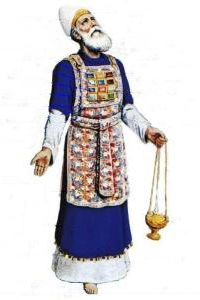
\includegraphics[width=50mm,scale=1.5]{Extras/Melchisedec.jpg}
\vspace{0.4in}  % Create a title for the document and write it in bold font
\LARGE{\textbf{\date}} % Again, do a line break
\linebreak 
% Create a subtitle \large{with Outlines, Statistics, Cross References, and Notes}
\vspace{0.5in}
\begin{flushleft}
\LARGE{Day \#30: Sunday, 30 January 2022   \\}\vspace{0.25in}
\LARGE{Exodus 37-38 Psalm 30 Proverb 30}
\end{flushleft}
\vspace{0.6in}
\bigskip

\normalsize{Xenia, Oh.\\}
\normalsize{created: \today}
\vspace{1.3in}

\end{flushright}
\end{titlepage}

%%%%%%%%%%%%
%%%%%%%%%%%%
%%%%%%%%%%%%

%\titleJE

\newpage 

\tableofcontents\hypertarget{TOC}{}
\listoffigures
\listoftables

\hyphenation{A-bim-e-lech bre-thren E-phra-im  Gib-e-o-nites Jer-u-sa-lem through-out Phil-i-stines The-o-phil-us Am-a-le-kites ven-geance Mesh-el-e-mi-ah onan-ism Phar-a-oh thoughts grev-ous-ness Hach-a-liah adul-ter-er Shad-rach}

%\fcolorbox{black}{bone}{TEXT}
%%%%%%%%%%%%%%%%% EXTRA COLORS
%%%%%%%%%%%%%%%%% EXTRA COLORS
%%%%%%%%%%%%%%%%% EXTRA COLORS
\definecolor{champagne}{rgb}{0.97,0.91,0.81}
\definecolor{bone}{rgb}{0.89,0.85,0.79}

\definecolor{ForestGreen}{rgb}{0.00,0.29,0.098}
\definecolor{GIVING}{cmyk}{1,0.0,0.72,.1}

\definecolor{MLPE}{cmyk}{1,1,0,.45}
\definecolor{SOCCER}{cmyk}{.77, 0, .42, .49}
\definecolor{PAYBILL}{cmyk}{0,0.83,0.76,0.07}
\definecolor{SERMON}{cmyk}{.14,.9,0,.30} % aka seance \href{http://www.flatuicolorpicker.com/purple-cmyk-color-model/}{seance}
\definecolor{BIBLE}{cmyk}{0,.17,.74,.17}
\definecolor{WORKBLUE}{cmyk}{1, .5, 0, .6}
\definecolor{myOrange}{cmyk}{0, .4, .98, .03}
\definecolor{myTan}{cmyk}{0.0,.07,.17,.10}
\definecolor{myRed}{cmyk}{0,1,1,0}
\definecolor{myWhite}{cmyk}{0,0,0,0}
\definecolor{BLUESoD}{cmyk}{.97,.84,0,.04}
\definecolor{WHITE}{cmyk}{0,0,0,0}
\definecolor{OLDGOLD}{cmyk}{0.05,0.3,1.00,0}
\definecolor{CASTLETON}{cmyk}{1,0,0.31,0.66}
\definecolor{cadmiumgreen}{rgb}{0.0, 0.42, 0.24}
\definecolor{jungle}{rgb}{0.203,0.4882,0.1718}
\definecolor{MYGOLD}{rgb}{1,.84,0}

\definecolor{MYLIGHTGRAY}{rgb}{.85,.85,.85}

\definecolor{codegreen}{rgb}{0,0.6,0}
\definecolor{codegray}{rgb}{0.5,0.5,0.5}
\definecolor{codepurple}{rgb}{0.58,0,0.82}
\definecolor{backcolour}{rgb}{0.95,0.95,0.92}



\mdfdefinestyle{MyFrame}{%
    linecolor=blue,
    outerlinewidth=2pt,
    roundcorner=5pt,
    innertopmargin=\baselineskip,
    innerbottommargin=\baselineskip,
    innerrightmargin=10pt,
    innerleftmargin=10pt,
    backgroundcolor=gray!25!white}


\mdfdefinestyle{MyFrame2}{%
    linecolor=black,
    outerlinewidth=2pt,
    roundcorner=5pt,
    innertopmargin=\baselineskip,
    innerbottommargin=\baselineskip,
    innerrightmargin=10pt,
    innerleftmargin=10pt,
    backgroundcolor=yellow!25!white}



%%%%%
%% for PFTTIS list
%%%%%

%%% And Joseph said unto
\index[PFTTIS]{And Joseph said unto!Genesis!Gen 40:008}
\index[PFTTIS]{And Joseph said unto!Genesis!Gen 40:012}
\index[PFTTIS]{And Joseph said unto!Genesis!Gen 41:025}
\index[PFTTIS]{And Joseph said unto!Genesis!Gen 42:014}
\index[PFTTIS]{And Joseph said unto!Genesis!Gen 42:018}
\index[PFTTIS]{And Joseph said unto!Genesis!Gen 44:015}
\index[PFTTIS]{And Joseph said unto!Genesis!Gen 45:003}
\index[PFTTIS]{And Joseph said unto!Genesis!Gen 45:004}
\index[PFTTIS]{And Joseph said unto!Genesis!Gen 46:031}
\index[PFTTIS]{And Joseph said unto!Genesis!Gen 48:009}
\index[PFTTIS]{And Joseph said unto!Genesis!Gen 48:018}
\index[PFTTIS]{And Joseph said unto!Genesis!Gen 50:019}
\index[PFTTIS]{And Joseph said unto!Genesis!Gen 50:024}


%%% a shadow
\index[PFTTIS]{a shadow!1Chronicles!1Chr 029:15}
\index[PFTTIS]{a shadow!Job!Job 008:09}
\index[PFTTIS]{a shadow!Job!Job 014:02}
\index[PFTTIS]{a shadow!Job!Job 017:07}
\index[PFTTIS]{a shadow!Psalm!Psa 102:011}
\index[PFTTIS]{a shadow!Psalm!Psa 144:004}
\index[PFTTIS]{a shadow!Ecclesiastes!Eccl 006:012}
\index[PFTTIS]{a shadow!Ecclesiastes!Eccl 008:013}
\index[PFTTIS]{a shadow!Isaiah!Isa 04:006}
\index[PFTTIS]{a shadow!Isaiah!Isa 25:004}
\index[PFTTIS]{a shadow!Jonah!Jnh 04:06}
\index[PFTTIS]{a shadow!Colossians!Col 02:017}
\index[PFTTIS]{a shadow!Hebews!Heb 10:001}

%%% blessed is the man
\index[PFTTIS]{blessed is the man!Psalm!Psa 001:001}
\index[PFTTIS]{blessed is the man!Psalm!Psa 032:002}
\index[PFTTIS]{blessed is the man!Psalm!Psa 034:008}
\index[PFTTIS]{blessed is the man!Psalm!Psa 065:004}
\index[PFTTIS]{blessed is the man!Psalm!Psa 084:005}
\index[PFTTIS]{blessed is the man!Psalm!Psa 084:012}
\index[PFTTIS]{blessed is the man!Psalm!Psa 094:012}
\index[PFTTIS]{blessed is the man!Psalm!Psa 112:001}
\index[PFTTIS]{blessed is the man!Proverbs!Pro 008:034}
\index[PFTTIS]{blessed is the man!Isaiah!Isa 056:002}
\index[PFTTIS]{blessed is the man!Jeremiah!Jer 017:007}
\index[PFTTIS]{blessed is the man!Romans!Rom 004:008}
\index[PFTTIS]{blessed is the man!James!Jam 001:012}


%%% carry them
\index[PFTTIS]{carry them!Leviticus!Lev 14:045}
\index[PFTTIS]{carry them!Numbers!Num 11:012}
\index[PFTTIS]{carry them!Joshua!Jsh 04:003}
\index[PFTTIS]{carry them!1Samuel!1Sam 20:040}
\index[PFTTIS]{carry them!1Kings!1Kng 08:046}
\index[PFTTIS]{carry them!2Chronicles!2Chr 06:036}
\index[PFTTIS]{carry them!Ezra!Ezra 05:015}
\index[PFTTIS]{carry them!Isaiah!Isa 40:011}
\index[PFTTIS]{carry them!Isaiah!Isa 41:016}
\index[PFTTIS]{carry them!Isaiah!Isa 57:013}
\index[PFTTIS]{carry them!Jeremiah!Jer 20:004}
\index[PFTTIS]{carry them!Jeremiah!Jer 20:005}
\index[PFTTIS]{carry them!Jeremiah!Jer 43:012}


\index[PFTTIS]{good tidings!2Samuel!2Sam 18:027}
\index[PFTTIS]{good tidings!1Kings!1Ki 01:042}
\index[PFTTIS]{good tidings!2Kings!2Ki 07:009 (2x)}
\index[PFTTIS]{good tidings!Isaiah!Isa 40:009 (2x)}
\index[PFTTIS]{good tidings!Isaiah!Isa 41:007}
\index[PFTTIS]{good tidings!Isaiah!Isa 52:007}
\index[PFTTIS]{good tidings!Isaiah!Isa 61:001}
\index[PFTTIS]{good tidings!Nahum!Nah 01:005}
\index[PFTTIS]{good tidings!Luke!Lk 02:010}
\index[PFTTIS]{good tidings!1Thessalonians!1Thess 03:006}


%%% dead body
\index[PFTTIS]{dead body!Leviticus!Lev 21:011}
\index[PFTTIS]{dead body!Numbers!Num 06:006}
\index[PFTTIS]{dead body!Numbers!Num 09:006}
\index[PFTTIS]{dead body!Numbers!Num 09:007}
\index[PFTTIS]{dead body!Numbers!Num 09:010}
\index[PFTTIS]{dead body!Numbers!Num 09:011}
\index[PFTTIS]{dead body!Numbers!Num 09:013}
\index[PFTTIS]{dead body!Numbers!Num 09:016}
\index[PFTTIS]{dead body!2Kings!2Ki 08:005}
\index[PFTTIS]{dead body!Isaiah!Isa 26:019}
\index[PFTTIS]{dead body!Jeremiah!Jer 26:023}
\index[PFTTIS]{dead body!Jeremiah!Jer 36:030}
\index[PFTTIS]{dead body!Haggai!Hag 02:013}

%%% great sea
\index[PFTTIS]{great sea!Numbers!Num 34:006}
\index[PFTTIS]{great sea!Numbers!Num 34:007}
\index[PFTTIS]{great sea!Joshua!Jos 01:004}
\index[PFTTIS]{great sea!Joshua!Jos 09:001}
\index[PFTTIS]{great sea!Joshua!Jos 15:012}
\index[PFTTIS]{great sea!Joshua!Jos 15:047}
\index[PFTTIS]{great sea!Joshua!Jos 23:004}
\index[PFTTIS]{great sea!Ezekiel!Eze 47:010}
\index[PFTTIS]{great sea!Ezekiel!Eze 47:015}
\index[PFTTIS]{great sea!Ezekiel!Eze 47:019}
\index[PFTTIS]{great sea!Ezekiel!Eze 47:020}
\index[PFTTIS]{great sea!Ezekiel!Eze 48:028}
\index[PFTTIS]{great sea!Daniel!Dan 07:002}


%%% have forsaken me
\index[PFTTIS]{have forsaken me!Judges!Jdg 10:013}
\index[PFTTIS]{have forsaken me!1Samuel!1Sam 08:008}
\index[PFTTIS]{have forsaken me!1Kings!1Ki 11:033}
\index[PFTTIS]{have forsaken me!2Kings!2Ki 22:017}
\index[PFTTIS]{have forsaken me!2Chronicles!2Chr 12:005}
\index[PFTTIS]{have forsaken me!2Chronicles!2Chr 34:025}
\index[PFTTIS]{have forsaken me!Jeremiah!Jer 01:016}
\index[PFTTIS]{have forsaken me!Jeremiah!Jer 02:013}
\index[PFTTIS]{have forsaken me!Jeremiah!Jer 05:007}
\index[PFTTIS]{have forsaken me!Jeremiah!Jer 05:019}
\index[PFTTIS]{have forsaken me!Jeremiah!Jer 16:011 (2x)}
\index[PFTTIS]{have forsaken me!Jeremiah!Jer 19:004}

%%% no king
\index[PFTTIS]{no king!Judges!Jdg 17:06}
\index[PFTTIS]{no king!Judges!Jdg 18:01}
\index[PFTTIS]{no king!Judges!Jdg 19:01}
\index[PFTTIS]{no king!Judges!Jdg 21:25}
\index[PFTTIS]{no king!1Kings!1Ki 22:47}
\index[PFTTIS]{no king!2Kings!2Ki 23:25}
\index[PFTTIS]{no king!Nehemiah!Neh 13:26}
\index[PFTTIS]{no king!Psalms!Psa 033:016}
\index[PFTTIS]{no king!Proverbs!Pro 30:27}
\index[PFTTIS]{no king!Daniel!Dan 02:10}
\index[PFTTIS]{no king!Hosea!Hos 10:03}
\index[PFTTIS]{no king!Micah!Mic 04:09}
\index[PFTTIS]{no king!John!Jhn 19:15}


%%% rebellious house
\index[PFTTIS]{rebellious house!Exodus!Exo 02:005}
\index[PFTTIS]{rebellious house!Exodus!Exo 02:006}
\index[PFTTIS]{rebellious house!Exodus!Exo 02:008}
\index[PFTTIS]{rebellious house!Exodus!Exo 03:009}
\index[PFTTIS]{rebellious house!Exodus!Exo 03:026}
\index[PFTTIS]{rebellious house!Exodus!Exo 03:027}
\index[PFTTIS]{rebellious house!Exodus!Exo 12:002 (2x)}
\index[PFTTIS]{rebellious house!Exodus!Exo 12:003}
\index[PFTTIS]{rebellious house!Exodus!Exo 12:009}
\index[PFTTIS]{rebellious house!Exodus!Exo 12:025}
\index[PFTTIS]{rebellious house!Exodus!Exo 17:012}
\index[PFTTIS]{rebellious house!Exodus!Exo 24:003}

%%% seek him
\index[PFTTIS]{seek him!Deuteronomy!Deu 04:029}\index[PFTTIS]{seek him!1Samuel!1Sam 23:025}
\index[PFTTIS]{seek him!1Chronicles!1Chr 28:009}
\index[PFTTIS]{seek him!2Chronicles!1Chr 15:002}
\index[PFTTIS]{seek him!Ezra!Ezr 08:022}
\index[PFTTIS]{seek him!Psalms!Psa 022:026}
\index[PFTTIS]{seek him!Psalms!Psa 024:006}
\index[PFTTIS]{seek him!Psalms!Psa 119:002}
\index[PFTTIS]{seek him!SoS!SoS 03:002}
\index[PFTTIS]{seek him!SoS!SoS 06:001}
\index[PFTTIS]{seek him!Hosea!Hos 07:010}
\index[PFTTIS]{seek him!Amos!Amo 05:008}
\index[PFTTIS]{seek him!Hebrews!Heb 11:0063}


%%% seek ye
\index[PFTTIS]{seek ye!Isaiah!Isa 34:016}
\index[PFTTIS]{seek ye!Isaiah!Isa 45:019}
\index[PFTTIS]{seek ye!Isaiah!Isa 55:006}
\index[PFTTIS]{seek ye!Amos!Amos 5:004}
\index[PFTTIS]{seek ye!John!John 1:38}
\index[PFTTIS]{seek ye!John!John 18:4}
\index[PFTTIS]{seek ye!John!John 18:7}
\index[PFTTIS]{seek ye!Matthew!Matt 6:33}
\index[PFTTIS]{seek ye!Numbers!Num 16:10}
\index[PFTTIS]{seek ye!Luke!Luke 12:31}
\index[PFTTIS]{seek ye!Luke!Luke 24:5}
\index[PFTTIS]{seek ye!Psalm!Psa 27:8}
\index[PFTTIS]{seek ye!Zephaniah!Zeph 2:3}

%%% the uncircumcised
\index[PFTTIS]{the uncircumcised!Genesis!Gen 17:014}
\index[PFTTIS]{the uncircumcised!Judges!Jdg 14:003}
\index[PFTTIS]{the uncircumcised!Judges!Jdg 15:018}
\index[PFTTIS]{the uncircumcised!2Samuel!2Sam 01:020}
\index[PFTTIS]{the uncircumcised!Isaiah!Isa 02:001}
\index[PFTTIS]{the uncircumcised!Jeremiah!Jer 09:025}
\index[PFTTIS]{the uncircumcised!Ezekiel!Eze 28:010}
\index[PFTTIS]{the uncircumcised!Ezekiel!Eze 31:018}
\index[PFTTIS]{the uncircumcised!Ezekiel!Eze 32:019}
\index[PFTTIS]{the uncircumcised!Ezekiel!Eze 32:027}
\index[PFTTIS]{the uncircumcised!Ezekiel!Eze 32:028}
\index[PFTTIS]{the uncircumcised!Ezekiel!Eze 32:029}
\index[PFTTIS]{the uncircumcised!Ezekiel!Eze 32:032}

%%% worship him
\index[PFTTIS]{worship him!Psalms!Psa 97:007}
\index[PFTTIS]{worship him!Zephaniah!Zeph 02:011}
\index[PFTTIS]{worship him!Matthew!Matt 02:002}
\index[PFTTIS]{worship him!Matthew!Matt 02:008}
\index[PFTTIS]{worship him!John!John 04:023}
\index[PFTTIS]{worship him!John!John 04:024 (2x)} 
\index[PFTTIS]{worship him!Acts!Acts 17:023}
\index[PFTTIS]{worship him!Hebrews!Heb 01:006}
\index[PFTTIS]{worship him!Revelation!Rev 04:010}
\index[PFTTIS]{worship him!Revelation!Rev 13:008}
\index[PFTTIS]{worship him!Revelation!Rev 14:007}
\index[PFTTIS]{worship him!Revelation!Rev 19:010}


%%%%%
%% for PFTTIS list
%%%%%

%%% afflictions
\index[WFTTIS]{afflictions!Psalms!Psa 34:019}
\index[WFTTIS]{afflictions!Psalms!Psa 132:001}
\index[WFTTIS]{afflictions!Acts!Acts 07:010}
\index[WFTTIS]{afflictions!Acts!Acts 20:023}
\index[WFTTIS]{afflictions!2Corinthians!2Cor 06:004}
\index[WFTTIS]{afflictions!Colossians!Col 01:024}
\index[WFTTIS]{afflictions!1Thessalonians!1Thess 03:003}
\index[WFTTIS]{afflictions!2Timothy!2Tim 01:008}
\index[WFTTIS]{afflictions!2Timothy!2Tim 03:011}
\index[WFTTIS]{afflictions!2Timothy!2Tim 04:005}
\index[WFTTIS]{afflictions!Hebrews!Heb 10:032}
\index[WFTTIS]{afflictions!Hebrews!Heb 10:033}
\index[WFTTIS]{afflictions!1Peter!1Pet 05:009}

%%% acsend
\index[WFTTIS]{acsend!Joshua!Jos 06:05}
\index[WFTTIS]{acsend!Psalm!Psa 024:003}
\index[WFTTIS]{acsend!Psalm!Psa 135:007}
\index[WFTTIS]{acsend!Psalm!Psa 139:008}
\index[WFTTIS]{acsend!Isaiah!Isa 14:013}
\index[WFTTIS]{acsend!Isaiah!Isa 14:014}
\index[WFTTIS]{acsend!Jeremiah!Jer 10:013}
\index[WFTTIS]{acsend!Jeremiah!Jer 51:016}
\index[WFTTIS]{acsend!Ezekiel!Eze 38:009}
\index[WFTTIS]{acsend!John!John 06:062}
\index[WFTTIS]{acsend!John!John 20:017}
\index[WFTTIS]{acsend!Romans!Rom 10:006}
\index[WFTTIS]{acsend!Revelation!Rev 17:008}

%%% Assyrian
\index[WFTTIS]{Assyrian!Isaiah!Isa 10:005}
\index[WFTTIS]{Assyrian!Isaiah!Isa 10:024}
\index[WFTTIS]{Assyrian!Isaiah!Isa 14:025}
\index[WFTTIS]{Assyrian!Isaiah!Isa 19:023}
\index[WFTTIS]{Assyrian!Isaiah!Isa 23:013}
\index[WFTTIS]{Assyrian!Isaiah!Isa 30:031}
\index[WFTTIS]{Assyrian!Isaiah!Isa 31:008}
\index[WFTTIS]{Assyrian!Isaiah!Isa 52:004}
\index[WFTTIS]{Assyrian!Ezekiel!Eze 31:003}
\index[WFTTIS]{Assyrian!Hosea!Hos 05:013}
\index[WFTTIS]{Assyrian!Hosea!Hos 11:005}
\index[WFTTIS]{Assyrian!Micah!Hos 05:005}
\index[WFTTIS]{Assyrian!Micah!Hos 05:006}

%%% blot
\index[WFTTIS]{blot!Exodus!Exo 32:032}
\index[WFTTIS]{blot!Exodus!Exo 32:033}
\index[WFTTIS]{blot!Numbers!Num 05:026}
\index[WFTTIS]{blot!Deuteronomy!Deut 09:014}
\index[WFTTIS]{blot!Deuteronomy!Deut 25:019}
\index[WFTTIS]{blot!Deuteronomy!Deut 29:020}
\index[WFTTIS]{blot!2Kings!2Ki 14:027}
\index[WFTTIS]{blot!Job!Job 31:007}
\index[WFTTIS]{blot!Psalms!Psa 51:001}
\index[WFTTIS]{blot!Psalms!Psa 51:009}
\index[WFTTIS]{blot!Proverbs!Pro 09:007}
\index[WFTTIS]{blot!Jeremiah!Jer 18:023}
\index[WFTTIS]{blot!Revelation!Rev 03:005}


%%% chain
\index[WFTTIS]{chain!Genesis!Gen 41:042}
\index[WFTTIS]{chain!1Kings!1Ki 07:017}
\index[WFTTIS]{chain!Psalms!Psa 73:006}
\index[WFTTIS]{chain!SoS!Sos 04:009}
\index[WFTTIS]{chain!Lamentations!Lam 03:007}
\index[WFTTIS]{chain!Ezekiel!Eze 07:023}
\index[WFTTIS]{chain!Ezekiel!Eze 16:011}
\index[WFTTIS]{chain!Daniel!Dan 05:007}
\index[WFTTIS]{chain!Daniel!Dan 05:016}
\index[WFTTIS]{chain!Daniel!Dan 05:029}
\index[WFTTIS]{chain!Acts!Acts 28:020}
\index[WFTTIS]{chain!2Timothy!2Tim 01:016}
\index[WFTTIS]{chain!Revelation!Rev 20:001}


%%% controversy
\index[WFTTIS]{controversy!Deuteronomy!Deu 17:008}
\index[WFTTIS]{controversy!Deuteronomy!Deu 19:017}
\index[WFTTIS]{controversy!Deuteronomy!Deu 21:005}
\index[WFTTIS]{controversy!Deuteronomy!Deu 25:001}
\index[WFTTIS]{controversy!2Samuel!2Sam 15:002}
\index[WFTTIS]{controversy!Isaiah!Isa 34:008}
\index[WFTTIS]{controversy!Jeremiah!Jer 25:031}
\index[WFTTIS]{controversy!Ezekiel!Eze 44:024}
\index[WFTTIS]{controversy!Hosea!Hos 04:001}
\index[WFTTIS]{controversy!Hosea!Hos 12:002}
\index[WFTTIS]{controversy!Micah!Mic 06:002 (2x)}
\index[WFTTIS]{controversy!1Timothy!1Tim 03:016}


%%% Dagon/Dagon's
\index[WFTTIS]{Dagon!Judges!Jdg 16:023}
\index[WFTTIS]{Dagon!1Samuel!1Sam 05:002 (2x)}
\index[WFTTIS]{Dagon!1Samuel!1Sam 05:003 (2x)}
\index[WFTTIS]{Dagon!1Samuel!1Sam 05:004 (3x)}
\index[WFTTIS]{Dagon!1Samuel!1Sam 05:005 (3x)}
\index[WFTTIS]{Dagon!1Samuel!1Sam 05:007}
\index[WFTTIS]{Dagon!1Chronicles!1Chr 10:010}

%%% disobedient
\index[WFTTIS]{disobedient!1Kings!1Ki 13:026}
\index[WFTTIS]{disobedient!Nehemiah!Neh 09:026}
\index[WFTTIS]{disobedient!Luke!Luke 01:017}
\index[WFTTIS]{disobedient!Acts!Acts 26:019}
\index[WFTTIS]{disobedient!Romans!Rom 01:030}
\index[WFTTIS]{disobedient!Romans!Rom 10:021}
\index[WFTTIS]{disobedient!1Timothy!1Tim 01:009}
\index[WFTTIS]{disobedient!2Timothy!2Tim 03:002}
\index[WFTTIS]{disobedient!Titus!Titus 01:016}
\index[WFTTIS]{disobedient!Titus!Titus 03:003}
\index[WFTTIS]{disobedient!1Peter!1Pet 02:007}
\index[WFTTIS]{disobedient!1Peter!1Pet 02:008}
\index[WFTTIS]{disobedient!1Peter!1Pet 03:020}


%%% doubt
\index[WFTTIS]{doubt!Genesis!Gen 37:033}
\index[WFTTIS]{doubt!Deuteronomy!Deu 28:066}
\index[WFTTIS]{doubt!Job!Job 12:002}
\index[WFTTIS]{doubt!Matthew!Matt 14:031}
\index[WFTTIS]{doubt!Matthew!Matt 21:021}
\index[WFTTIS]{doubt!Mark!Mk 11:023}
\index[WFTTIS]{doubt!Luke!Lk 11:020}
\index[WFTTIS]{doubt!John!Jhn 10:024}
\index[WFTTIS]{doubt!Acts!Acts 02:012}
\index[WFTTIS]{doubt!Acts!Acts 28:004}
\index[WFTTIS]{doubt!1Corinthians!1Cor 09:010}
\index[WFTTIS]{doubt!Galatians!Gal 04:020}
\index[WFTTIS]{doubt!1John!1Jhn 02:019}


%%% dungeon
\index[WFTTIS]{dungeon!Genesis!Gen 40:015}
\index[WFTTIS]{dungeon!Genesis!Gen 41:014}
\index[WFTTIS]{dungeon!Exodus!Exo 12:029}
\index[WFTTIS]{dungeon!Jeremiah!Jer 37:016}
\index[WFTTIS]{dungeon!Jeremiah!Jer 38:006 (2x)}
\index[WFTTIS]{dungeon!Jeremiah!Jer 38:007}
\index[WFTTIS]{dungeon!Jeremiah!Jer 38:009}
\index[WFTTIS]{dungeon!Jeremiah!Jer 38:010}
\index[WFTTIS]{dungeon!Jeremiah!Jer 38:011}
\index[WFTTIS]{dungeon!Jeremiah!Jer 38:013}
\index[WFTTIS]{dungeon!Lamentations!Lam 03:053}
\index[WFTTIS]{dungeon!Lamentations!Lam 03:055}


%%% error
\index[WFTTIS]{error!2Samuel!2Sam 06:007}
\index[WFTTIS]{error!Job!Job 19:004}
\index[WFTTIS]{error!Ecclesiastes!Ecc 05:006}
\index[WFTTIS]{error!Ecclesiastes!Ecc 10:005}
\index[WFTTIS]{error!Isaiah!Isa 32:006}
\index[WFTTIS]{error!Daniel!Dan 06:004}
\index[WFTTIS]{error!Matthew!Matt 27:064}
\index[WFTTIS]{error!Romans!Rom 01:027}
\index[WFTTIS]{error!James!Jam 05:020}
\index[WFTTIS]{error!2Peter!2Pet 02:018}
\index[WFTTIS]{error!2Peter!2Pet 03:017}
\index[WFTTIS]{error!1John!1Jn 04:006}
\index[WFTTIS]{error!Jude!Jude 01:011}

%%% fourish
\index[WFTTIS]{fourish!Psalms!Psa 072:007}
\index[WFTTIS]{fourish!Psalms!Psa 072:016}
\index[WFTTIS]{fourish!Psalms!Psa 092:007}
\index[WFTTIS]{fourish!Psalms!Psa 092:012}
\index[WFTTIS]{fourish!Psalms!Psa 092:013}
\index[WFTTIS]{fourish!Psalms!Psa 132:018}
\index[WFTTIS]{fourish!Proverbs!Pro 11:28}
\index[WFTTIS]{fourish!Proverbs!Pro 14:11}
\index[WFTTIS]{fourish!Ecclesiastes!Ecc 12:05}
\index[WFTTIS]{fourish!SongOfSolomon!SOS 07:12}
\index[WFTTIS]{fourish!Isaiah!Isa 17:11}
\index[WFTTIS]{fourish!Isaiah!Isa 66:14}
\index[WFTTIS]{fourish!Ezekiel!Eze 17:24}




%%% giants
\index[WFTTIS]{giants!Genesis!Gen 06:004}
\index[WFTTIS]{giants!Numbers!Num 13:033}
\index[WFTTIS]{giants!Deuteronomy!Deut 02:011}
\index[WFTTIS]{giants!Deuteronomy!Deut 02:021}
\index[WFTTIS]{giants!Deuteronomy!Deut 03:011}
\index[WFTTIS]{giants!Deuteronomy!Deut 03:013}
\index[WFTTIS]{giants!Joshua!Josh 12:004}
\index[WFTTIS]{giants!Joshua!Josh 13:012}
\index[WFTTIS]{giants!Joshua!Josh 15:008}
\index[WFTTIS]{giants!Joshua!Josh 17:015}
\index[WFTTIS]{giants!Joshua!Josh 16:016}

%%% good man
\index[WFTTIS]{good man!2 Samuel!2Sa 18:27}
%(1) Psalms 37:23 [5]
%(1) Psalms 112:5 [2]
%(1) Proverbs 12:2 [2]
%(1) Proverbs 13:22 [2]
%(1) Proverbs 14:14 [14]
%(1) Micah 7:2 [2]
%(1) Matthew 12:35 [2]
%(1) Luke 6:45 [2]
%(1) Luke 23:50 [15]
%(1) John 7:12 [17]
%(1) Acts 11:24 [5]
%(1) Romans 5:7 [14]

%%% Hinnom
\index[WFTTIS]{Hinnom!Joshua!Jsh 15:008}
\index[WFTTIS]{Hinnom!Joshua!Jsh 18:016}
\index[WFTTIS]{Hinnom!2Kings!2Ki 23:010}
\index[WFTTIS]{Hinnom!2Chronicles!2Chr 28:003}
\index[WFTTIS]{Hinnom!2Chronicles!2Chr 33:006}
\index[WFTTIS]{Hinnom!Nehemiah!Neh 11:030}
\index[WFTTIS]{Hinnom!Jeremiah!Jer 07:031}
\index[WFTTIS]{Hinnom!Jeremiah!Jer 07:032}
\index[WFTTIS]{Hinnom!Jeremiah!Jer 19:002}
\index[WFTTIS]{Hinnom!Jeremiah!Jer 19:006}
\index[WFTTIS]{Hinnom!Jeremiah!Jer 32:035}

%%% inclined
\index[WFTTIS]{inclined!Judges!Jdg 09:003}
\index[WFTTIS]{inclined!Psalms!Psa 040:001}
\index[WFTTIS]{inclined!Psalms!Psa 116:002}
\index[WFTTIS]{inclined!Psalms!Psa 119:112}
\index[WFTTIS]{inclined!Proverbs!Pro 05:13}
\index[WFTTIS]{inclined!Jeremiah!Jer 07:24}
\index[WFTTIS]{inclined!Jeremiah!Jer 07:26}
\index[WFTTIS]{inclined!Jeremiah!Jer 11:08}
\index[WFTTIS]{inclined!Jeremiah!Jer 17:23}
\index[WFTTIS]{inclined!Jeremiah!Jer 25:04}
\index[WFTTIS]{inclined!Jeremiah!Jer 34:14}
\index[WFTTIS]{inclined!Jeremiah!Jer 35:15}
\index[WFTTIS]{inclined!Jeremiah!Jer 44:05}


%%% laughed
\index[WFTTIS]{laughed!Genesis!Gen 17:017}
\index[WFTTIS]{laughed!Genesis!Gen 18:012}
\index[WFTTIS]{laughed!Genesis!Gen 18:015}
\index[WFTTIS]{laughed!2Kings!2Ki 19:021}
\index[WFTTIS]{laughed!2Chronicles!2Chr 30:010}
\index[WFTTIS]{laughed!Nehemiah!Neh 02:019}
\index[WFTTIS]{laughed!Job!Job 12:004}
\index[WFTTIS]{laughed!Job!Job 29:024}
\index[WFTTIS]{laughed!Isaiah!Isa 37:022}
\index[WFTTIS]{laughed!Ezekiel!Ezek 23:032}
\index[WFTTIS]{laughed!Matthew!Matt 09:024}
\index[WFTTIS]{laughed!Mark!Mk 05:040}
\index[WFTTIS]{laughed!Luke!Lk 08:053}

%%% liar
\index[WFTTIS]{liar!Job!Job 24:025}
\index[WFTTIS]{liar!Proverbs!Pro 17:004}
\index[WFTTIS]{liar!Proverbs!Pro 19:022}
\index[WFTTIS]{liar!Proverbs!Pro 30:006}
\index[WFTTIS]{liar!Jeremiah!Jer 15:018}
\index[WFTTIS]{liar!John!Jhn 08:044}
\index[WFTTIS]{liar!John!Jhn 08:055}
\index[WFTTIS]{liar!Romans!Rom 03:004}
\index[WFTTIS]{liar!1John!1Jhn 01:010}
\index[WFTTIS]{liar!1John!1Jhn 02:004}
\index[WFTTIS]{liar!1John!1Jhn 02:022}
\index[WFTTIS]{liar!1John!1Jhn 04:020}
\index[WFTTIS]{liar!1John!1Jhn 05:010}

%%% palsy
\index[WFTTIS]{palsy!Matthew!Matt 04:024}
\index[WFTTIS]{palsy!Matthew!Matt 08:006}
\index[WFTTIS]{palsy!Matthew!Matt 09:002}
\index[WFTTIS]{palsy!Matthew!Matt 09:006}
\index[WFTTIS]{palsy!Mark!Mk 02:003}
\index[WFTTIS]{palsy!Mark!Mk 02:004}
\index[WFTTIS]{palsy!Mark!Mk 02:005}
\index[WFTTIS]{palsy!Mark!Mk 02:009}
\index[WFTTIS]{palsy!Mark!Mk 02:010}
\index[WFTTIS]{palsy!Luke!Lk 05:018}
\index[WFTTIS]{palsy!Luke!Lk 05:024}
\index[WFTTIS]{palsy!Acts!Acts 09:033}

%%% Profitable
\index[WFTTIS]{profitable!Job!Job 22:002 (2x)}
\index[WFTTIS]{profitable!Ecclesiastes!Ecc 10:010}
\index[WFTTIS]{profitable!Isaiah!Isa 44:010}
\index[WFTTIS]{profitable!Jeremiah!Jer 13:007}
\index[WFTTIS]{profitable!Matthew!Matt 05:029}
\index[WFTTIS]{profitable!Matthew!Matt 05:030}
\index[WFTTIS]{profitable!Acts!Acts 20:020}
\index[WFTTIS]{profitable!1Timothy!1Tim 04:008}
\index[WFTTIS]{profitable!2Timothy!2Tim 03:016}
\index[WFTTIS]{profitable!2Timothy!2Tim 04:011}
\index[WFTTIS]{profitable!Titus!Titus 03:008}
\index[WFTTIS]{profitable!Philemon!Phlm 01:011}

%%% Rechab
\index[WFTTIS]{Rechab!2Samuel!2Sam 04:002}
\index[WFTTIS]{Rechab!2Samuel!2Sam 04:005}
\index[WFTTIS]{Rechab!2Samuel!2Sam 04:006}
\index[WFTTIS]{Rechab!2Samuel!2Sam 04:009}
\index[WFTTIS]{Rechab!2KIngs!2Ki 10:015}
\index[WFTTIS]{Rechab!2KIngs!2Ki 10:023}
\index[WFTTIS]{Rechab!1Chronicles!1Chr 02:055}
\index[WFTTIS]{Rechab!Nehemiah!Neh 03:014}
\index[WFTTIS]{Rechab!Jeremiah!Jer 35:006}
\index[WFTTIS]{Rechab!Jeremiah!Jer 35:008}
\index[WFTTIS]{Rechab!Jeremiah!Jer 35:014}
\index[WFTTIS]{Rechab!Jeremiah!Jer 35:016}
\index[WFTTIS]{Rechab!Jeremiah!Jer 35:019}

%%% serpents
\index[WFTTIS]{serpents!Exodus!Exo 07:012}
\index[WFTTIS]{serpents!Numbers!Num 21:006}
\index[WFTTIS]{serpents!Numbers!Num 21:007}
\index[WFTTIS]{serpents!Deuteronomy!Deu 08:015}
\index[WFTTIS]{serpents!Deuteronomy!Deu 32:024}
\index[WFTTIS]{serpents!Jeremiah!Jer 08:017}
\index[WFTTIS]{serpents!Matthew!Matt 10:016}
\index[WFTTIS]{serpents!Matthew!Matt 23:033}
\index[WFTTIS]{serpents!Mark!Mk 16:018}
\index[WFTTIS]{serpents!Luke!Lk 10:019}
\index[WFTTIS]{serpents!1Corinthians!1Cor 10:009}
\index[WFTTIS]{serpents!James!Jas 03:007}
\index[WFTTIS]{serpents!Revelation!Rev 09:019}

%%% short
\index[WFTTIS]{short!Numbers!Num 11:023}
\index[WFTTIS]{short!2Kings!2Ki 10:032}
\index[WFTTIS]{short!Job!Job 17:012}
\index[WFTTIS]{short!Job!Job 20:005}
\index[WFTTIS]{short!Psalms!Psa 89:047}
\index[WFTTIS]{short!Romans!Rom 03:023}
\index[WFTTIS]{short!Romans!Rom 09:028  (2x)}
\index[WFTTIS]{short!1Corinthians!1Cor 07:029}
\index[WFTTIS]{short!1Thessalonians!1Thess 02:017}
\index[WFTTIS]{short!Hebrews!Heb 04:001}
\index[WFTTIS]{short!Revelation!Rev 12:012}
\index[WFTTIS]{short!Revelation!Rev 17:010}

%%% smiteth
\index[WFTTIS]{smiteth!Exodus!Exo 21:012}
\index[WFTTIS]{smiteth!Exodus!Exo 21:15}
\index[WFTTIS]{smiteth!Deuteronomy!Dt 25:11}
\index[WFTTIS]{smiteth!Deuteronomy!Dt 27:24}
\index[WFTTIS]{smiteth!Joshua!Jsh 15:16}
\index[WFTTIS]{smiteth!Judges!Jdg 15:16}
\index[WFTTIS]{smiteth!2 Samuel!2Sa 05:08}
\index[WFTTIS]{smiteth!1Chronicles!1Chr 11:06}
\index[WFTTIS]{smiteth!Job!1Chr 26:12}
\index[WFTTIS]{smiteth!Isaiah!Isa 09:13}
\index[WFTTIS]{smiteth!Lamentations!Lam 03:30}
\index[WFTTIS]{smiteth!Ezekiel!Eze 07:09}
\index[WFTTIS]{smiteth!Luke!Lk 06:29}



%%% vanities
\index[WFTTIS]{vanities!Deuteronomy!Deut 21:021}
\index[WFTTIS]{vanities!1Kings!1Ki 16:013}
\index[WFTTIS]{vanities!1Kings!1Ki 16:026}
\index[WFTTIS]{vanities!Psalms!Psa 031:006}
\index[WFTTIS]{vanities!Ecclesiastes!Ecc 01:002 (2x)}
\index[WFTTIS]{vanities!Ecclesiastes!Ecc 05:007}
\index[WFTTIS]{vanities!Ecclesiastes!Ecc 12:008}
\index[WFTTIS]{vanities!Jeremiah!Jer 08:019}
\index[WFTTIS]{vanities!Jeremiah!Jer 10:008}
\index[WFTTIS]{vanities!Jeremiah!Jer 14:022}
\index[WFTTIS]{vanities!Jonah!Jnh 02:008}
\index[WFTTIS]{vanities!Acts!Acts 14:015}



%%%%%
%% for PFTTIS list
%%%%%

%%% worm
\index[WFITV]{worm!Exodus!Exo 16:024}
\index[WFITV]{worm!Job!Job 17:014}
\index[WFITV]{worm!Job!Job 24:029}
\index[WFITV]{worm!Job!Job 25:005 (2x)}
\index[WFITV]{worm!Psalms!Psa 022:006}
\index[WFITV]{worm!Isaiah!Isa 14:011}
\index[WFITV]{worm!Isaiah!Isa 41:014}
\index[WFITV]{worm!Isaiah!Isa 51:008}
\index[WFITV]{worm!Isaiah!Isa 66:024}
\index[WFITV]{worm!Jonah!Jnh 04:007}
\index[WFITV]{worm!Mark!Mk 09:044}
\index[WFITV]{worm!Mark!Mk 09:046}
\index[WFITV]{worm!Mark!Mk 09:048}


%\subsubsection{Title}
%\textbf{Introduction:} Isaiah 46 
%\index[speaker]{Speaker!Isaiah 49 (Title}
%\index[series]{Book (Speaker)!IPassage (Title)}
%\index[date]{2017/07/09!Isaiah 49 (Title)}
%\begin{compactenum}[I.]
%    \item  \textbf{Point} \index[scripture]{Isaiah!IPassage} (IPassage)
%\end{compactenum}




  

%\chapter{Today's Readings}

\normalsize
 
\begin{center}
\begin{longtable}{|p{0.45in}|p{0.25in}|p{0.4in}|p{2.8in}|c|c|}
\caption[Today's Chapters]{Today's Chapters}\label{table:Today's Chapters} \\
\hline 
\multicolumn{1}{|c|}{\textbf{Chap}} & 
\multicolumn{1}{|c|}{\textbf{\#}} & 
\multicolumn{1}{|c|}{\textbf{Rvrs} } & 
\multicolumn{1}{|c|}{\textbf{address numerics}} & 
\multicolumn{1}{|c|}{\textbf{Vss}} & 
\multicolumn{1}{|c|}{\textbf{wds}}  \\ 
\hline 
\endfirsthead

 
\multicolumn{6}{c}
{{\bfseries \tablename\ \thetable{} -- continued from previous page}} \\  
\hline \multicolumn{1}{|c|}{\textbf{Chap}} & \multicolumn{1}{|c|}{\textbf{\#}} & \multicolumn{1}{|c|}{\textbf{Rev}} & \multicolumn{1}{|c|}{\textbf{addr Num}} & \multicolumn{1}{|c|}{\textbf{Verses}} & \multicolumn{1}{|c|}{\textbf{words}}  \\ \hline \endhead
 
%\hline \multicolumn{6}{|r|}{{Continued}} \\ \hline
\endfoot 
%Exo 20 & 70 & 1120 & 70 = 2 * 5 * 7; 1120 = 2 * 2 * 2 * 2 * 2 * 5 * 7 & 26 & 561 \\ \hline
%Exo 21 & 71 & 1119 & 71 is prime; 1119 = 3 * 373 & 36 & 893 \\ \hline \hline
%Exo 22 & 72 & 1118 &72 = 2 * 2 * 3 * 3; 1118 = 2 * 13 * 17 & 31 & 790 \\ \hline
%Exo 23 & 73 & 1117 & 73 is prime; 1117 is & 33 & 827 \\ \hline
%Exo 24 & 74 & 1116 & 74 = 2 * 37; 1116 = 2 8 2 * 3 * 3 * 31 & 18 & 492 \\ \hline \hline
%Exo 25 & 75 & 1115 & 75 = 3 * 5 * 5; 1115 = 5 * 223 & 40 & 926 \\ \hline
%Exo 26 & 76 & 1114 & 76 = 2 * 2 * 19; 1114 = 2 * 557 & 37 & 937 \\ \hline
%Exo 27 & 77 & 1113 & 77 = 7 * 11; 1113 = 3 * 7 * 53 & 18 & 492 \\ \hline \hline
%Exo 28 & 78 & 1112 & 78 = 2 * 3 * 13; 1112 = 2 * 2 * 2 * 139 & 43 & 1235 \\ \hline
%Exo 28 & 79 & 1111 & 79 is prime; 1111 = 11 * 101 & 46 & 1341 \\ \hline
%Exo 30 & 80 & 1110 & 80 = 2 * 2 * 2 * 2 * 5; 1110 = 2 * 3 * 5 * 37 & 38 & 970 \\ \hline \hline
%Exo 31 & 81 & 1109 & 81 = 3 * 3 * 3 * 3; 1109 is prime & 18 & 438 \\ \hline
%Exo 32 & 82 & 1108 & 82 = 1 * 41; 1108 = 2 * 2 * 277 & 35 & 1093 \\ \hline
%Exo 33 & 83 & 1107 & 83 is prime; 1107 = 3 * 3 * 3 * 41  & 23 & 710 \\ \hline \hline
Exo 34 & 84 & 1106 & 84 = 2 * 2 * 3 * 7; 1106 = 3 * 7 * 79 & 18 & 438 \\ \hline
Exo 35 & 85 & 1105 & 85 = 5 * 17; 1105 = 5 * 13 * 17 & 35 & 1093 \\ \hline
Exo 36 & 86 & 1104 & 86 = 2 * 43; 1104 = 2 * 2 * 2 * 2 * 3 * 23 & 23 & 710 \\ \hline \hline

%Psa 23 & 501 & 690 & 501 is prime; 690 = 2 * 3 * 5 * 23 & 31 & 246 \\ \hline \hline
%Psa 24 & 502 & 689 & 502 = 2 * 251 ; 689  = 13 * 53 & 10 & 178 \\ \hline \hline
%Psa 25 & 503 & 688 &  503 is prime ; 688  = 2 * 2 * 2 * 2 * 43 & 22 & 342 \\ \hline 
%Psa 27 & 504 & 687 &  504 = 2 * 2 * 2 * 3 * 3 * 7 ; 687  = 3 * 229 & 14 & 340 \\ \hline \hline
%Psa 28 & 505 & 686 &  505 = 5 * 101 ; 686  = 2 * 7 * 7 * 7 & 9 & 201 \\ \hline \hline
Psa 29 & 506 & 685 &  506 = 2 * 11 * 23 ; 685 = 5 * 137 & 11 & 179 \\ \hline \hline

%Pro 23 & 651 & 539 & 651 = 3 * 7 * 31; 539 = 7 * 7 * 11 & 35 & 566 \\ \hline \hline
%Pro 24 & 652 & 538 & 652 = 2 * 2 * 163; 538 = 2 * 269 & 34 & 580 \\ \hline \hline
%Pro 25 & 653 & 537 & 653 is prime; 537 = 3 * 179 & 28 & 522 \\ \hline \hline
%Pro 27 & 654 & 536 & 654 = 2 * 3 * 109; 536 = 2 * 2 * 2 * 67 & 23 & 460 \\ \hline 
%Pro 28 & 655 & 535 & 655 = 5 * 131; 535 = 5 * 107& 28 & 527 \\ \hline 
Pro 29 & 656 & 534 & 656 = 2 * 2 * 2 * 2 * 41; 534 = 2 * 3 * 89 & 27 & 425 \\ \hline 

\end{longtable}
\end{center}

%%%%%%%%%%%%%%%%%%%%%%%%%%%%%%%%%%%%%%%%%%%%
%%%%%%%%%%%%%%%%%%%%%%%%%%%%%%%%%%%%%%%%%%%%

\begin{center}
\begin{longtable}{|p{0.7in}|p{3.8in}|}
\caption[Today's Chapter Summaries]{Today's Chapter Summaries}\label{table:Today's Chapter Summaries} \\
\hline \multicolumn{1}{|c|}{\textbf{Chap}} & \multicolumn{1}{|c|}{\textbf{comments}}  \\ \hline 
\endfirsthead
 
\multicolumn{2}{c}
{{\bfseries \tablename\ \thetable{} -- continued from previous page}} \\  
\hline \multicolumn{1}{|c|}{\textbf{Chap}} & \multicolumn{1}{|c|}{\textbf{comments}}  \\ \hline 
 \\ \hline 
\endhead
 
%\hline \multicolumn{2}{|r|}{{}} \\ \hline
\endfoot 
Exo 34 & Moses made new tablets for the law. The LORD spoke to him and made a covenant with Israel. When Moses returned his face was shining.  \\ \hline
Exo 35 & Moses told the Israelites to keep the Sabbath. He called for craftsmen to make the tabernacle. The people gave gifts for the work. \\ \hline
Exo 36 & The people gave more than enough. The craftsmen made the curtains. Bezalel made the curtains, the boards, the veil and the pillars. \\ \hline

Psa 29 &  The people gave more than enough. The craftsmen made the curtains. Bezalel made the curtains, the boards, the veil and the pillars. \\ \hline
Prov 29 & By justice a king builds up the land. Whether a fool rages or laughs, there is no peace. Correct your son and he will give you rest.\\ \hline

\end{longtable}
\end{center}



%%%%%%%%%%%%%%%%%%%%%%%%%%%

\chapter{Exodus Introduction}

\begin{center}
\begin{longtable}{p{0.25in}|p{1.5in}|p{2.75in}}
\caption[Words  Thirteen Times in the Exodus Chapters]{Words Thirteen Times in the Exodus Chapters} \label{table:Stats-EXO-13-TIC} \\ 
\hline \multicolumn{1}{|c|}{\textbf{Chapter}} & 
\multicolumn{1}{|c|}{\textbf{Word(s)}} & 
\multicolumn{1}{|c|}{\textbf{Comment}}   \\ \hline 
\endfirsthead
 
\multicolumn{3}{c}
{{\bfseries \tablename\ \thetable{} -- continued from previous page}} \\  
\hline \multicolumn{1}{|c|}{\textbf{Chapter}} & 
\multicolumn{1}{|c|}{\textbf{Word(s)}} & 
\multicolumn{1}{|c|}{\textbf{Comment}}  \\ \hline 
\endhead
 
\hline \multicolumn{3}{|r|}{{Continued as needed}} \\ \hline
\endfoot 
3 & said &  \\ \hline
4 & hand, it &   \\ \hline
6 & LORD, Moses &   \\ \hline
8 & said, shall, that &   \\ \hline
9 & Moses, all , not, unto &   \\ \hline
10 & said &   \\ \hline
12 & day, land, unto, LORD &   \\  \hline
13 & shall &   \\ \hline  
16 & said, shall &   \\ \hline
18 & law, that, they &   \\ \hline
19 & to &   \\ \hline
21 & ox, that &   \\ \hline
26 & shall & \\ \hline
28 & ephod, that, them, LORD & \\ \hline
29 & LORD, that, unto & \\ \hline
30 & LORD, that  & \\ \hline
32 & he, that  & \\ \hline
33 & thou  & \\ \hline
34 & Moses  & \\ \hline
35 & all  & \\ \hline
36 & tabernacle  & \\ \hline
37 & of  & \\ \hline
38 & were, pillars, sockets  & \\ \hline
39 & gold, it  & \\ \hline
40 & Moses, put, tent  & \\ \hline
\hline \hline
%Total & 594 & 224 & 22 & 12



\end{longtable}
\end{center}


\begin{center}
\begin{longtable}{c|c|p{3.5in}}
\caption[Verses with 13 Words]{Verses with 13 Words} \label{table:Stats-EXO-13-VWTW} \\ 
\hline \multicolumn{1}{|c|}{\textbf{Chapter}} & 
\multicolumn{1}{|c|}{\textbf{Verse}} & 
\multicolumn{1}{|l|}{\textbf{Comment}}   \\ \hline 
\endfirsthead
 
\multicolumn{3}{c}
{{\bfseries \tablename\ \thetable{} -- continued from previous page}} \\  
\hline \multicolumn{1}{|c|}{\textbf{Chapter}} & 
\multicolumn{1}{|c|}{\textbf{Verse}} & 
\multicolumn{1}{|l|}{\textbf{Comment}}  \\ \hline 
\endhead
 
\hline \multicolumn{3}{|r|}{{Continued as needed}} \\ \hline
\endfoot 
1 & 1:8 & a new king in Egypt, who knew not Joseph \\ \hline
6 & 6:2 & God says, ``I am the LORD.'' \\ \hline
7 & 7:6 & Moses and Aaron did as the LORD commanded them \\ 
7 & 2:25 & Seven days fulfilled after the Lord had smitten the river \\ \hline
9 & 9:2 & If Pharaoh refuses to the Israel go  \\ \hline
10 & 10:27 & But the LORD hardened Pharaoh’s heart, and he would not let them go.  \\ \hline
13 & 13:10 &  Thou shalt therefore keep this ordinance in his season from year to year. \\ \hline
15 & 15:05 &  The depths have covered them: they sank into the bottom as a stone. \\ \hline
16 & 16:17& And the children of Israel did so, and gathered, some more, some less. \\ \hline
17 & 17:13 & And Joshua discomfited Amalek and his people with the edge of the sword.\\ \hline
22 & 22:28 &  Thou shalt not revile the gods, nor curse the ruler of thy people.\\ \hline
24 & 24:15 &  And Moses went up into the mount, and a cloud covered the mount.\\ \hline
25 & 25:8 &  And let them make me a sanctuary; that I may dwell among them.\\ 
25 & 25:13 &  And thou shalt make staves of shittim wood, and overlay them with gold.\\ 
25 & 25:38 &  And the tongs thereof, and the snuffdishes thereof, shall be of pure gold.\\ \hline
26 & 26:15 &  And thou shalt make boards for the tabernacle of shittim wood standing up.\\ 
26 & 26:22 & And for the sides of the tabernacle westward thou shalt make six boards.\\ \hline
28 & 28:18 & And the second row shall be an emerald, a sapphire, and a diamond.\\ \hline
30 & 30:19 & For Aaron and his sons shall wash their hands and their feet
thereat:\\ \hline
%34 &  & none \\ \hline
%35 &  & none \\ \hline
%36 &  & none \\ \hline
37 & 37:28  &And he made the staves of shittim wood, and overlaid them with brass. \\ \hline
38 & 38:06  & And he made the staves of shittim wood, and overlaid them with brass. \\ \hline
39 & 39:35  & The ark of the testimony, and the staves thereof, and the mercy seat, \\ \hline
40 & 40:25  &  \\ \hline


\hline \hline
%Total & 594 & 224 & 22 & 12



\end{longtable}
\end{center}

\newpage
\begin{figure}
\begin{center}
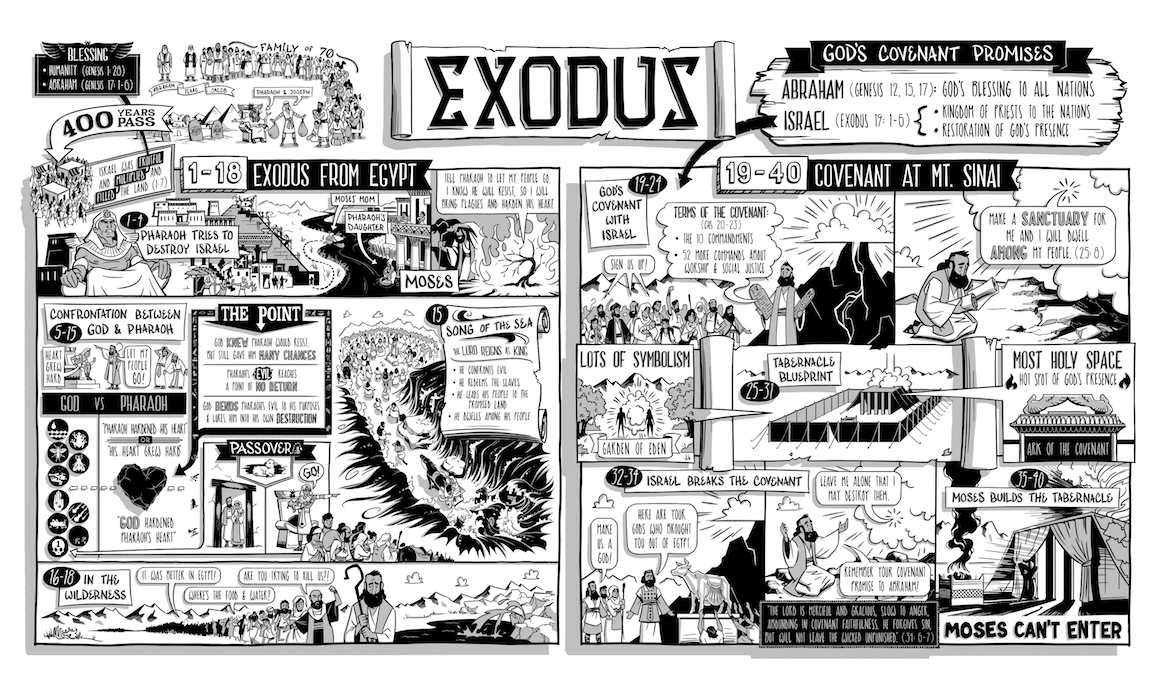
\includegraphics[scale=0.5, angle=90]{02OT-Exodus/References/BibleProject-Exodus.png}
\caption[Exodus from the Bible Project]{Exodus from the Bible Project}
\label{fig:Exodus from the Bible Project}
\end{center}
\end{figure}

\newpage
\begin{figure}
\begin{center}
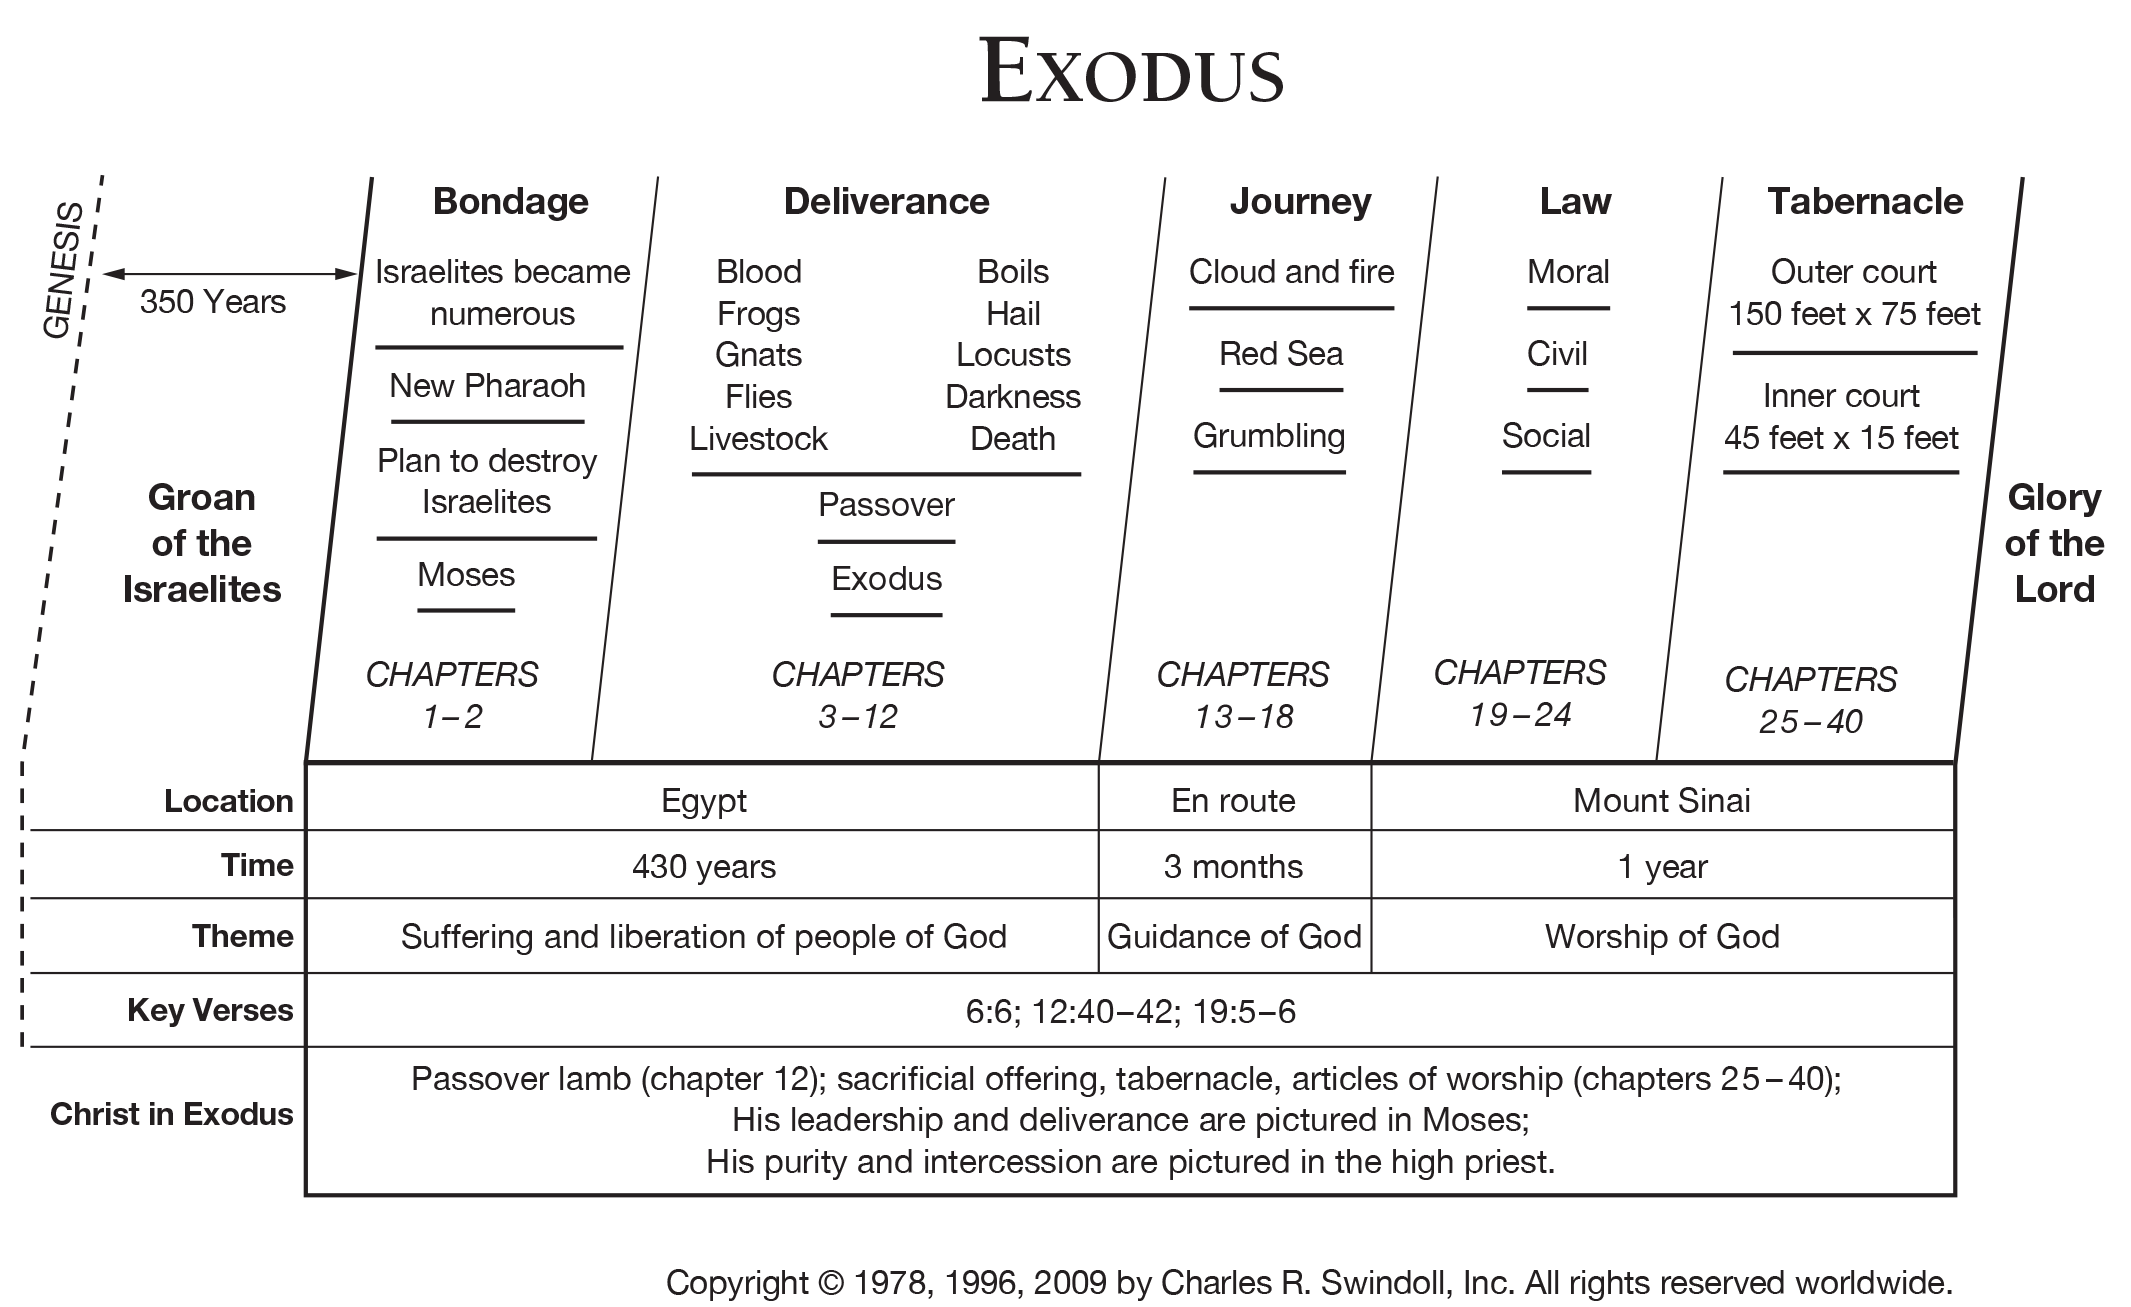
\includegraphics[scale=0.3, angle=90]{02OT-Exodus/References/Swindoll-Exodus.png}
\caption[Exodus by Swindoll]{Genesis by Exodus}
\label{fig:Exodus by Swindoll}
\end{center}
\end{figure}

\newpage
\begin{figure}
\begin{center}
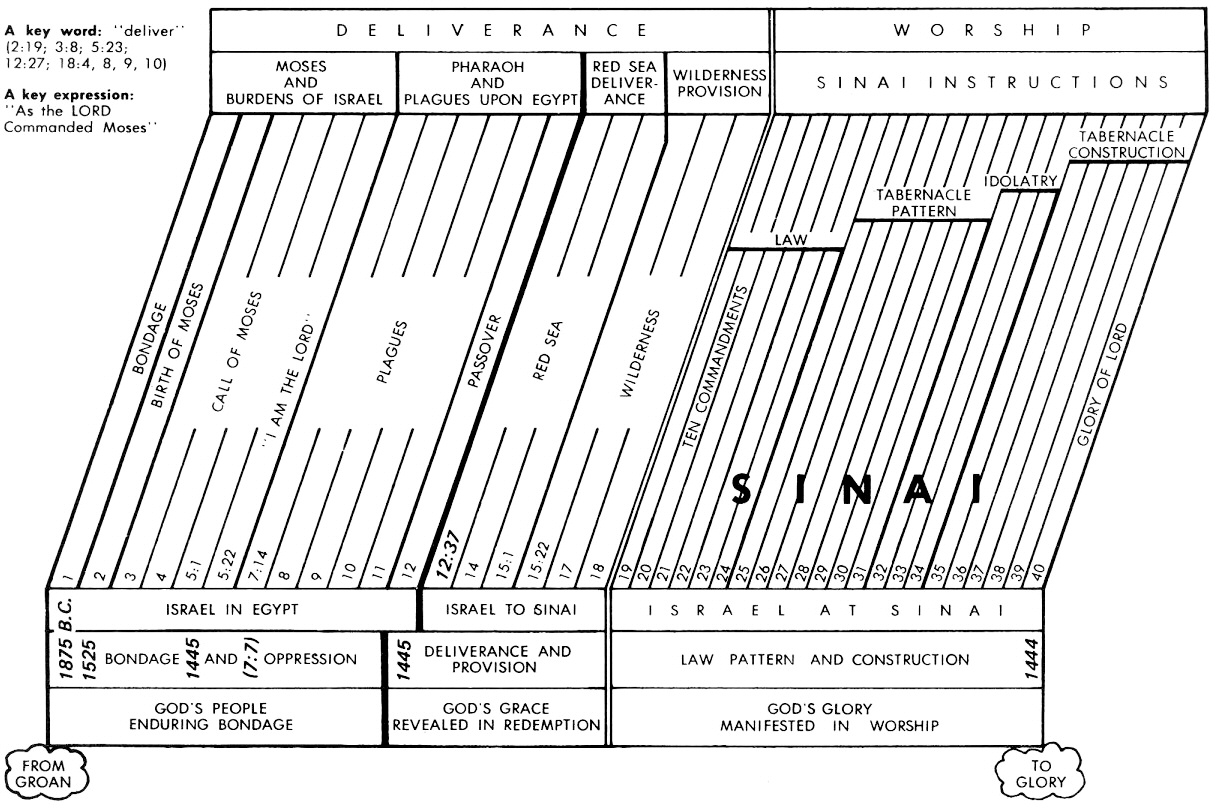
\includegraphics[scale=1.7, angle=90]{02OT-Exodus/References/Jensen-Exodus.png}
\caption[Exodus by Jensen]{Exodus by Jensen}
\label{fig:Exodus by Jensen}
\end{center}
\end{figure}

\newpage
\begin{figure}
\begin{center}
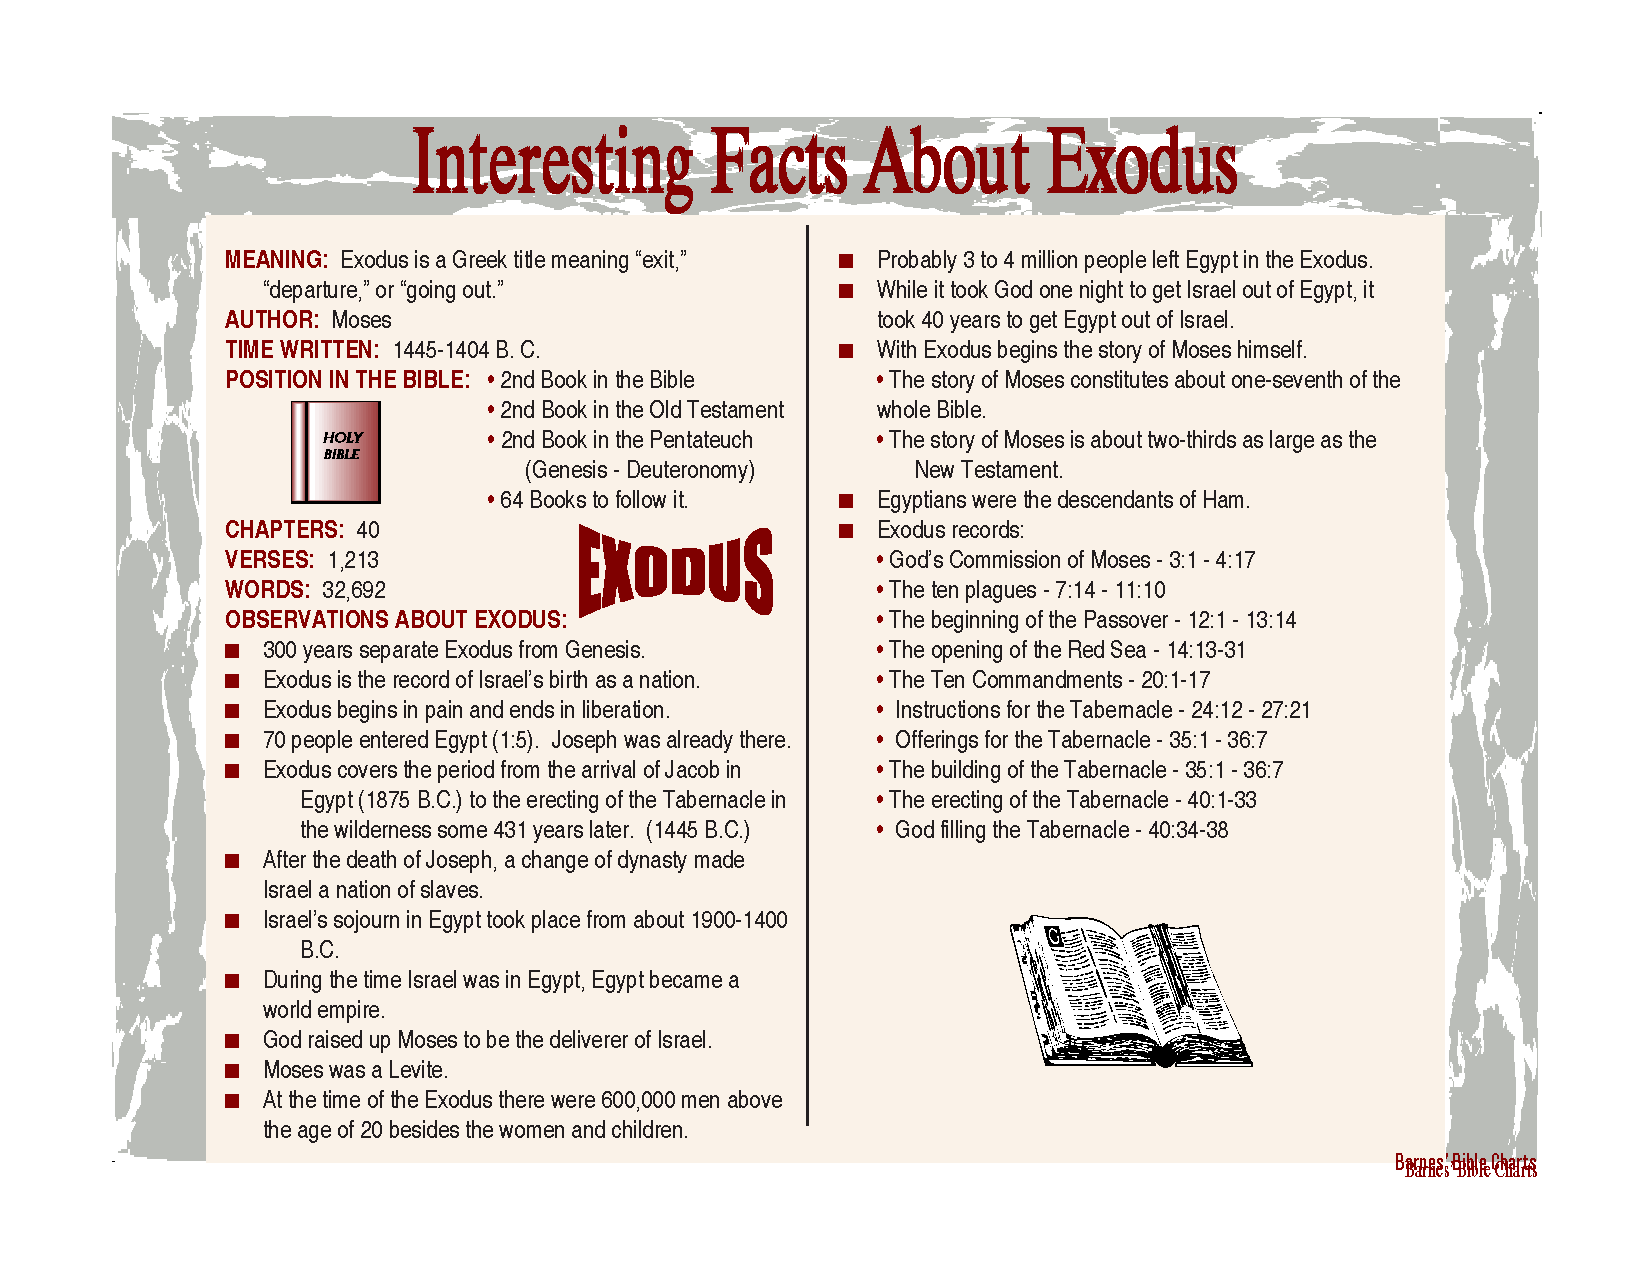
\includegraphics[scale=0.6, angle=90]{02OT-Exodus/References/interestingfactsaboutexodus.pdf}
\caption[Interesting Facts About Exodus]{Interesting Facts About Exodus}
\label{fig:Interesting Facts About Exodus}
\end{center}
\end{figure}




\chapter{Exodus 37}

\marginpar{\scriptsize \centering \fcolorbox{bone}{lime}{\textbf{ABOUT THE ARK}}\\ (Exodus 37:1--29) 
\begin{compactenum}[I.][8]
    \item \textbf{Crafted} with Skill \index[scripture]{Exodus!Exo 37:01}(Exo 37:1)  
    \item \textbf{Crowned} \index[scripture]{Exodus!Exo 37:02}(Exodus 37:2)    \item \textbf{Covered} with Gold \index[scripture]{Exodus!Exo 37:02}\index[scripture]{Exodus!Exo 37:03}\index[scripture]{Exodus!Exo 37:04}\index[scripture]{Exodus!Exo 37:06}(Exo 37:2, 3, 4, 6)
    \item Measured in \textbf{Cubits} \index[scripture]{Exodus!Exo 37:01}\index[scripture]{Exodus!Exo 37:06}(Exo 37:1, 6)
    \item \textbf{Carried} with gold-plated wood \index[scripture]{Exodus!Exo 37:04}\index[scripture]{Exodus!Exo 37:05}(Exo 37:4, 5)
    \item \textbf{Accompanied} by Cherubim \index[scripture]{Exodus!Exo 37:07}\index[scripture]{Exodus!Exo 37:08}\index[scripture]{Exodus!Exo 37:09}(Exo 37:7, 8, 9)
    \item \textbf{Contains} a mercy-seat \index[scripture]{Exodus!Exo 37:06}\index[scripture]{Exodus!Exo 37:07}\index[scripture]{Exodus!Exo 37:08}\index[scripture]{Exodus!Exo 37:09}(Exo 37:6, 7, 8, 9)  
\end{compactenum} }



\footnote{\textcolor[cmyk]{0.99998,1,0,0}{\hyperlink{TOC}{Return to end of Table of Contents.}}}\footnote{\href{https://audiobible.com/bible/exodus_37.html}{\textcolor[cmyk]{0.99998,1,0,0}{Exodus 37 Audio}}}\textcolor[cmyk]{0.99998,1,0,0}{And \fcolorbox{bone}{lime}{Bezaleel made the ark} \fcolorbox{bone}{bone}{\emph{of}} shittim wood: two \fcolorbox{bone}{lime}{cubits} and a half \emph{was} the length of it, and a cubit and a half the breadth of it, and a cubit and a half the height of it:}
[2] \textcolor[cmyk]{0.99998,1,0,0}{And he overlaid it with pure gold within and without, and made a \fcolorbox{bone}{lime}{crown of gold} to it round about.}
[3] \textcolor[cmyk]{0.99998,1,0,0}{And he cast for it four rings of gold, \emph{to} \emph{be} \emph{set} by the four corners of it; even two rings upon the one side of it, and two rings upon the other side of it.}
[4] \textcolor[cmyk]{0.99998,1,0,0}{And he made staves \fcolorbox{bone}{bone}{\emph{of}} shittim wood, and overlaid them with gold.}
[5] \textcolor[cmyk]{0.99998,1,0,0}{And he put the staves into the rings by the sides of the ark, to bear the ark.}\\
\\
\P \textcolor[cmyk]{0.99998,1,0,0}{And  the mercy seat \fcolorbox{bone}{bone}{\emph{of}} pure gold: two cubits and a half \emph{was} the length thereof, and one cubit and a half the breadth thereof.}
[7] \textcolor[cmyk]{0.99998,1,0,0}{And he made two \fcolorbox{bone}{lime}{cherubims} \fcolorbox{bone}{bone}{\emph{of}} gold, beaten out of one piece made he them, on the two ends of the \fcolorbox{bone}{lime}{mercy seat};}
[8] \textcolor[cmyk]{0.99998,1,0,0}{One cherub on the end on this side, and another cherub on the \emph{other} end on that side: out of the mercy seat made he the cherubims on the two ends thereof.}
[9] \textcolor[cmyk]{0.99998,1,0,0}{And the cherubims spread out \emph{their} wings on high, \emph{and} covered with their wings over the mercy seat, with their faces one to another; \emph{even} to the mercy seatward were the faces of the cherubims.}\\
\\
\P \textcolor[cmyk]{0.99998,1,0,0}{And he made the table \fcolorbox{bone}{bone}{\emph{of}} shittim wood: two cubits \emph{was} the length thereof, and a cubit the breadth thereof, and a cubit and a half the height thereof:}
[11] \textcolor[cmyk]{0.99998,1,0,0}{And he overlaid it with pure gold, and made thereunto a crown of gold round about.}
[12] \textcolor[cmyk]{0.99998,1,0,0}{Also he made thereunto a border of an handbreadth round about; and made a crown of gold for the border thereof round about.}
[13] \textcolor[cmyk]{0.99998,1,0,0}{And he cast for it four rings of gold, and put the rings upon the four corners that \emph{were} in the four feet thereof.}
[14] \textcolor[cmyk]{0.99998,1,0,0}{Over against the border were the rings, the places for the staves to bear the table.}
[15] \textcolor[cmyk]{0.99998,1,0,0}{And he made the staves \fcolorbox{bone}{bone}{\emph{of}} shittim wood, and overlaid them with gold, to bear the table.}
[16] \textcolor[cmyk]{0.99998,1,0,0}{And he made the vessels which \emph{were} upon the table, his dishes, and his spoons, and his bowls, and his covers to cover withal, \fcolorbox{bone}{bone}{\emph{of}} pure gold.}\\
\\
\P \textcolor[cmyk]{0.99998,1,0,0}{And he made the candlestick \fcolorbox{bone}{bone}{\emph{of}} pure gold: \fcolorbox{bone}{bone}{\emph{of}} beaten work made he the candlestick; his shaft, and his branch, his bowls, his knops, and his flowers, were of the same:}
[18] \textcolor[cmyk]{0.99998,1,0,0}{And six branches going out of the sides thereof; three branches of the candlestick out of the one side thereof, and three branches of the candlestick out of the other side thereof:}
[19] \textcolor[cmyk]{0.99998,1,0,0}{Three bowls made after the fashion of almonds in one branch, a knop and a flower; and three bowls made like almonds in another branch, a knop and a flower: so throughout the six branches going out of the candlestick.}
[20] \textcolor[cmyk]{0.99998,1,0,0}{And in the candlestick \emph{were} four bowls made like almonds, his knops, and his flowers:}
[21] \textcolor[cmyk]{0.99998,1,0,0}{And a knop under two branches of the same, and a knop under two branches of the same, and a knop under two branches of the same, according to the six branches going out of it.}
[22] \textcolor[cmyk]{0.99998,1,0,0}{Their knops and their branches were of the same: all of it \emph{was} one beaten work \fcolorbox{bone}{bone}{\emph{of}} pure gold.}
[23] \textcolor[cmyk]{0.99998,1,0,0}{And he made his seven lamps, and his snuffers, and his snuffdishes, \fcolorbox{bone}{bone}{\emph{of}} pure gold.}
[24] \textcolor[cmyk]{0.99998,1,0,0}{\emph{Of} a talent of pure gold made he it, and all the vessels thereof.}\\
\\
\P \textcolor[cmyk]{0.99998,1,0,0}{And he made the incense altar \fcolorbox{bone}{bone}{\emph{of}} shittim wood: the length of it \emph{was} a cubit, and the breadth of it a cubit; \emph{it} \emph{was} foursquare; and two cubits \emph{was} the height of it; the horns thereof were of the same.}
[26] \textcolor[cmyk]{0.99998,1,0,0}{And he overlaid it with pure gold, \emph{both} the top of it, and the sides thereof round about, and the horns of it: also he made unto it a crown of gold round about.}
[27] \textcolor[cmyk]{0.99998,1,0,0}{And he made two rings of gold for it under the crown thereof, by the two corners of it, upon the two sides thereof, to be places for the staves to bear it withal.}
[28] \textcolor[cmyk]{0.99998,1,0,0}{And he made the staves \fcolorbox{bone}{bone}{\emph{of}} shittim wood, and overlaid them with gold.}\\
\\
\P \textcolor[cmyk]{0.99998,1,0,0}{And he made the holy anointing oil, and the pure incense of sweet spices, according to the work of the apothecary.}
\index[NWIV]{38!Exodus!Exo 37:1}\index[AWIP]{And!Exodus!Exo 37:1}\index[AWIP]{Bezaleel!Exodus!Exo 37:1}\index[AWIP]{made!Exodus!Exo 37:1}\index[AWIP]{the!Exodus!Exo 37:1}\index[AWIP]{the!Exodus!Exo 37:1 (2)}\index[AWIP]{the!Exodus!Exo 37:1 (3)}\index[AWIP]{the!Exodus!Exo 37:1 (4)}\index[AWIP]{ark!Exodus!Exo 37:1}\index[AWIP]{\emph{of}!Exodus!Exo 37:1}\index[AWIP]{shittim!Exodus!Exo 37:1}\index[AWIP]{wood!Exodus!Exo 37:1}\index[AWIP]{two!Exodus!Exo 37:1}\index[AWIP]{cubits!Exodus!Exo 37:1}\index[AWIP]{and!Exodus!Exo 37:1}\index[AWIP]{and!Exodus!Exo 37:1 (2)}\index[AWIP]{and!Exodus!Exo 37:1 (3)}\index[AWIP]{and!Exodus!Exo 37:1 (4)}\index[AWIP]{and!Exodus!Exo 37:1 (5)}\index[AWIP]{a!Exodus!Exo 37:1}\index[AWIP]{a!Exodus!Exo 37:1 (2)}\index[AWIP]{a!Exodus!Exo 37:1 (3)}\index[AWIP]{a!Exodus!Exo 37:1 (4)}\index[AWIP]{a!Exodus!Exo 37:1 (5)}\index[AWIP]{half!Exodus!Exo 37:1}\index[AWIP]{half!Exodus!Exo 37:1 (2)}\index[AWIP]{half!Exodus!Exo 37:1 (3)}\index[AWIP]{\emph{was}!Exodus!Exo 37:1}\index[AWIP]{length!Exodus!Exo 37:1}\index[AWIP]{of!Exodus!Exo 37:1}\index[AWIP]{of!Exodus!Exo 37:1 (2)}\index[AWIP]{of!Exodus!Exo 37:1 (3)}\index[AWIP]{it!Exodus!Exo 37:1}\index[AWIP]{it!Exodus!Exo 37:1 (2)}\index[AWIP]{it!Exodus!Exo 37:1 (3)}\index[AWIP]{cubit!Exodus!Exo 37:1}\index[AWIP]{cubit!Exodus!Exo 37:1 (2)}\index[AWIP]{breadth!Exodus!Exo 37:1}\index[AWIP]{height!Exodus!Exo 37:1}\index[AWIP]{\emph{of}!Exodus!Exo 37:1}\index[AWIP]{\emph{was}!Exodus!Exo 37:1}

\index[NWIV]{20!Exodus!Exo 37:2}\index[AWIP]{And!Exodus!Exo 37:2}\index[AWIP]{he!Exodus!Exo 37:2}\index[AWIP]{overlaid!Exodus!Exo 37:2}\index[AWIP]{it!Exodus!Exo 37:2}\index[AWIP]{it!Exodus!Exo 37:2 (2)}\index[AWIP]{with!Exodus!Exo 37:2}\index[AWIP]{pure!Exodus!Exo 37:2}\index[AWIP]{gold!Exodus!Exo 37:2}\index[AWIP]{gold!Exodus!Exo 37:2 (2)}\index[AWIP]{within!Exodus!Exo 37:2}\index[AWIP]{and!Exodus!Exo 37:2}\index[AWIP]{and!Exodus!Exo 37:2 (2)}\index[AWIP]{without!Exodus!Exo 37:2}\index[AWIP]{made!Exodus!Exo 37:2}\index[AWIP]{a!Exodus!Exo 37:2}\index[AWIP]{crown!Exodus!Exo 37:2}\index[AWIP]{of!Exodus!Exo 37:2}\index[AWIP]{to!Exodus!Exo 37:2}\index[AWIP]{round!Exodus!Exo 37:2}\index[AWIP]{about!Exodus!Exo 37:2}

\index[NWIV]{36!Exodus!Exo 37:3}\index[AWIP]{And!Exodus!Exo 37:3}\index[AWIP]{he!Exodus!Exo 37:3}\index[AWIP]{cast!Exodus!Exo 37:3}\index[AWIP]{for!Exodus!Exo 37:3}\index[AWIP]{it!Exodus!Exo 37:3}\index[AWIP]{it!Exodus!Exo 37:3 (2)}\index[AWIP]{it!Exodus!Exo 37:3 (3)}\index[AWIP]{it!Exodus!Exo 37:3 (4)}\index[AWIP]{four!Exodus!Exo 37:3}\index[AWIP]{four!Exodus!Exo 37:3 (2)}\index[AWIP]{rings!Exodus!Exo 37:3}\index[AWIP]{rings!Exodus!Exo 37:3 (2)}\index[AWIP]{rings!Exodus!Exo 37:3 (3)}\index[AWIP]{of!Exodus!Exo 37:3}\index[AWIP]{of!Exodus!Exo 37:3 (2)}\index[AWIP]{of!Exodus!Exo 37:3 (3)}\index[AWIP]{of!Exodus!Exo 37:3 (4)}\index[AWIP]{gold!Exodus!Exo 37:3}\index[AWIP]{\emph{to}!Exodus!Exo 37:3}\index[AWIP]{\emph{be}!Exodus!Exo 37:3}\index[AWIP]{\emph{set}!Exodus!Exo 37:3}\index[AWIP]{by!Exodus!Exo 37:3}\index[AWIP]{the!Exodus!Exo 37:3}\index[AWIP]{the!Exodus!Exo 37:3 (2)}\index[AWIP]{the!Exodus!Exo 37:3 (3)}\index[AWIP]{corners!Exodus!Exo 37:3}\index[AWIP]{even!Exodus!Exo 37:3}\index[AWIP]{two!Exodus!Exo 37:3}\index[AWIP]{two!Exodus!Exo 37:3 (2)}\index[AWIP]{upon!Exodus!Exo 37:3}\index[AWIP]{upon!Exodus!Exo 37:3 (2)}\index[AWIP]{one!Exodus!Exo 37:3}\index[AWIP]{side!Exodus!Exo 37:3}\index[AWIP]{side!Exodus!Exo 37:3 (2)}\index[AWIP]{and!Exodus!Exo 37:3}\index[AWIP]{other!Exodus!Exo 37:3}\index[AWIP]{\emph{to}!Exodus!Exo 37:3}\index[AWIP]{\emph{be}!Exodus!Exo 37:3}\index[AWIP]{\emph{set}!Exodus!Exo 37:3}

\index[NWIV]{12!Exodus!Exo 37:4}\index[AWIP]{And!Exodus!Exo 37:4}\index[AWIP]{he!Exodus!Exo 37:4}\index[AWIP]{made!Exodus!Exo 37:4}\index[AWIP]{staves!Exodus!Exo 37:4}\index[AWIP]{\emph{of}!Exodus!Exo 37:4}\index[AWIP]{shittim!Exodus!Exo 37:4}\index[AWIP]{wood!Exodus!Exo 37:4}\index[AWIP]{and!Exodus!Exo 37:4}\index[AWIP]{overlaid!Exodus!Exo 37:4}\index[AWIP]{them!Exodus!Exo 37:4}\index[AWIP]{with!Exodus!Exo 37:4}\index[AWIP]{gold!Exodus!Exo 37:4}\index[AWIP]{\emph{of}!Exodus!Exo 37:4}

\index[NWIV]{18!Exodus!Exo 37:5}\index[AWIP]{And!Exodus!Exo 37:5}\index[AWIP]{he!Exodus!Exo 37:5}\index[AWIP]{put!Exodus!Exo 37:5}\index[AWIP]{the!Exodus!Exo 37:5}\index[AWIP]{the!Exodus!Exo 37:5 (2)}\index[AWIP]{the!Exodus!Exo 37:5 (3)}\index[AWIP]{the!Exodus!Exo 37:5 (4)}\index[AWIP]{the!Exodus!Exo 37:5 (5)}\index[AWIP]{staves!Exodus!Exo 37:5}\index[AWIP]{into!Exodus!Exo 37:5}\index[AWIP]{rings!Exodus!Exo 37:5}\index[AWIP]{by!Exodus!Exo 37:5}\index[AWIP]{sides!Exodus!Exo 37:5}\index[AWIP]{of!Exodus!Exo 37:5}\index[AWIP]{ark!Exodus!Exo 37:5}\index[AWIP]{ark!Exodus!Exo 37:5 (2)}\index[AWIP]{to!Exodus!Exo 37:5}\index[AWIP]{bear!Exodus!Exo 37:5}

\index[NWIV]{27!Exodus!Exo 37:6}\index[AWIP]{And!Exodus!Exo 37:6}\index[AWIP]{he!Exodus!Exo 37:6}\index[AWIP]{made!Exodus!Exo 37:6}\index[AWIP]{the!Exodus!Exo 37:6}\index[AWIP]{the!Exodus!Exo 37:6 (2)}\index[AWIP]{the!Exodus!Exo 37:6 (3)}\index[AWIP]{mercy!Exodus!Exo 37:6}\index[AWIP]{seat!Exodus!Exo 37:6}\index[AWIP]{\emph{of}!Exodus!Exo 37:6}\index[AWIP]{pure!Exodus!Exo 37:6}\index[AWIP]{gold!Exodus!Exo 37:6}\index[AWIP]{two!Exodus!Exo 37:6}\index[AWIP]{cubits!Exodus!Exo 37:6}\index[AWIP]{and!Exodus!Exo 37:6}\index[AWIP]{and!Exodus!Exo 37:6 (2)}\index[AWIP]{and!Exodus!Exo 37:6 (3)}\index[AWIP]{a!Exodus!Exo 37:6}\index[AWIP]{a!Exodus!Exo 37:6 (2)}\index[AWIP]{half!Exodus!Exo 37:6}\index[AWIP]{half!Exodus!Exo 37:6 (2)}\index[AWIP]{\emph{was}!Exodus!Exo 37:6}\index[AWIP]{length!Exodus!Exo 37:6}\index[AWIP]{thereof!Exodus!Exo 37:6}\index[AWIP]{thereof!Exodus!Exo 37:6 (2)}\index[AWIP]{one!Exodus!Exo 37:6}\index[AWIP]{cubit!Exodus!Exo 37:6}\index[AWIP]{breadth!Exodus!Exo 37:6}\index[AWIP]{\emph{of}!Exodus!Exo 37:6}\index[AWIP]{\emph{was}!Exodus!Exo 37:6}

\index[NWIV]{23!Exodus!Exo 37:7}\index[AWIP]{And!Exodus!Exo 37:7}\index[AWIP]{he!Exodus!Exo 37:7}\index[AWIP]{he!Exodus!Exo 37:7 (2)}\index[AWIP]{made!Exodus!Exo 37:7}\index[AWIP]{made!Exodus!Exo 37:7 (2)}\index[AWIP]{two!Exodus!Exo 37:7}\index[AWIP]{two!Exodus!Exo 37:7 (2)}\index[AWIP]{cherubims!Exodus!Exo 37:7}\index[AWIP]{\emph{of}!Exodus!Exo 37:7}\index[AWIP]{gold!Exodus!Exo 37:7}\index[AWIP]{beaten!Exodus!Exo 37:7}\index[AWIP]{out!Exodus!Exo 37:7}\index[AWIP]{of!Exodus!Exo 37:7}\index[AWIP]{of!Exodus!Exo 37:7 (2)}\index[AWIP]{one!Exodus!Exo 37:7}\index[AWIP]{piece!Exodus!Exo 37:7}\index[AWIP]{them!Exodus!Exo 37:7}\index[AWIP]{on!Exodus!Exo 37:7}\index[AWIP]{the!Exodus!Exo 37:7}\index[AWIP]{the!Exodus!Exo 37:7 (2)}\index[AWIP]{ends!Exodus!Exo 37:7}\index[AWIP]{mercy!Exodus!Exo 37:7}\index[AWIP]{seat!Exodus!Exo 37:7}\index[AWIP]{\emph{of}!Exodus!Exo 37:7}

\index[NWIV]{32!Exodus!Exo 37:8}\index[AWIP]{One!Exodus!Exo 37:8}\index[AWIP]{cherub!Exodus!Exo 37:8}\index[AWIP]{cherub!Exodus!Exo 37:8 (2)}\index[AWIP]{on!Exodus!Exo 37:8}\index[AWIP]{on!Exodus!Exo 37:8 (2)}\index[AWIP]{on!Exodus!Exo 37:8 (3)}\index[AWIP]{on!Exodus!Exo 37:8 (4)}\index[AWIP]{on!Exodus!Exo 37:8 (5)}\index[AWIP]{the!Exodus!Exo 37:8}\index[AWIP]{the!Exodus!Exo 37:8 (2)}\index[AWIP]{the!Exodus!Exo 37:8 (3)}\index[AWIP]{the!Exodus!Exo 37:8 (4)}\index[AWIP]{the!Exodus!Exo 37:8 (5)}\index[AWIP]{end!Exodus!Exo 37:8}\index[AWIP]{end!Exodus!Exo 37:8 (2)}\index[AWIP]{this!Exodus!Exo 37:8}\index[AWIP]{side!Exodus!Exo 37:8}\index[AWIP]{side!Exodus!Exo 37:8 (2)}\index[AWIP]{and!Exodus!Exo 37:8}\index[AWIP]{another!Exodus!Exo 37:8}\index[AWIP]{\emph{other}!Exodus!Exo 37:8}\index[AWIP]{that!Exodus!Exo 37:8}\index[AWIP]{out!Exodus!Exo 37:8}\index[AWIP]{of!Exodus!Exo 37:8}\index[AWIP]{mercy!Exodus!Exo 37:8}\index[AWIP]{seat!Exodus!Exo 37:8}\index[AWIP]{made!Exodus!Exo 37:8}\index[AWIP]{he!Exodus!Exo 37:8}\index[AWIP]{cherubims!Exodus!Exo 37:8}\index[AWIP]{two!Exodus!Exo 37:8}\index[AWIP]{ends!Exodus!Exo 37:8}\index[AWIP]{thereof!Exodus!Exo 37:8}\index[AWIP]{\emph{other}!Exodus!Exo 37:8}

\index[NWIV]{35!Exodus!Exo 37:9}\index[AWIP]{And!Exodus!Exo 37:9}\index[AWIP]{the!Exodus!Exo 37:9}\index[AWIP]{the!Exodus!Exo 37:9 (2)}\index[AWIP]{the!Exodus!Exo 37:9 (3)}\index[AWIP]{the!Exodus!Exo 37:9 (4)}\index[AWIP]{the!Exodus!Exo 37:9 (5)}\index[AWIP]{cherubims!Exodus!Exo 37:9}\index[AWIP]{cherubims!Exodus!Exo 37:9 (2)}\index[AWIP]{spread!Exodus!Exo 37:9}\index[AWIP]{out!Exodus!Exo 37:9}\index[AWIP]{\emph{their}!Exodus!Exo 37:9}\index[AWIP]{wings!Exodus!Exo 37:9}\index[AWIP]{wings!Exodus!Exo 37:9 (2)}\index[AWIP]{on!Exodus!Exo 37:9}\index[AWIP]{high!Exodus!Exo 37:9}\index[AWIP]{\emph{and}!Exodus!Exo 37:9}\index[AWIP]{covered!Exodus!Exo 37:9}\index[AWIP]{with!Exodus!Exo 37:9}\index[AWIP]{with!Exodus!Exo 37:9 (2)}\index[AWIP]{their!Exodus!Exo 37:9}\index[AWIP]{their!Exodus!Exo 37:9 (2)}\index[AWIP]{over!Exodus!Exo 37:9}\index[AWIP]{mercy!Exodus!Exo 37:9}\index[AWIP]{mercy!Exodus!Exo 37:9 (2)}\index[AWIP]{seat!Exodus!Exo 37:9}\index[AWIP]{faces!Exodus!Exo 37:9}\index[AWIP]{faces!Exodus!Exo 37:9 (2)}\index[AWIP]{one!Exodus!Exo 37:9}\index[AWIP]{to!Exodus!Exo 37:9}\index[AWIP]{to!Exodus!Exo 37:9 (2)}\index[AWIP]{another!Exodus!Exo 37:9}\index[AWIP]{\emph{even}!Exodus!Exo 37:9}\index[AWIP]{seatward!Exodus!Exo 37:9}\index[AWIP]{were!Exodus!Exo 37:9}\index[AWIP]{of!Exodus!Exo 37:9}\index[AWIP]{\emph{their}!Exodus!Exo 37:9}\index[AWIP]{\emph{and}!Exodus!Exo 37:9}\index[AWIP]{\emph{even}!Exodus!Exo 37:9}

\index[NWIV]{29!Exodus!Exo 37:10}\index[AWIP]{And!Exodus!Exo 37:10}\index[AWIP]{he!Exodus!Exo 37:10}\index[AWIP]{made!Exodus!Exo 37:10}\index[AWIP]{the!Exodus!Exo 37:10}\index[AWIP]{the!Exodus!Exo 37:10 (2)}\index[AWIP]{the!Exodus!Exo 37:10 (3)}\index[AWIP]{the!Exodus!Exo 37:10 (4)}\index[AWIP]{table!Exodus!Exo 37:10}\index[AWIP]{\emph{of}!Exodus!Exo 37:10}\index[AWIP]{shittim!Exodus!Exo 37:10}\index[AWIP]{wood!Exodus!Exo 37:10}\index[AWIP]{two!Exodus!Exo 37:10}\index[AWIP]{cubits!Exodus!Exo 37:10}\index[AWIP]{\emph{was}!Exodus!Exo 37:10}\index[AWIP]{length!Exodus!Exo 37:10}\index[AWIP]{thereof!Exodus!Exo 37:10}\index[AWIP]{thereof!Exodus!Exo 37:10 (2)}\index[AWIP]{thereof!Exodus!Exo 37:10 (3)}\index[AWIP]{and!Exodus!Exo 37:10}\index[AWIP]{and!Exodus!Exo 37:10 (2)}\index[AWIP]{and!Exodus!Exo 37:10 (3)}\index[AWIP]{a!Exodus!Exo 37:10}\index[AWIP]{a!Exodus!Exo 37:10 (2)}\index[AWIP]{a!Exodus!Exo 37:10 (3)}\index[AWIP]{cubit!Exodus!Exo 37:10}\index[AWIP]{cubit!Exodus!Exo 37:10 (2)}\index[AWIP]{breadth!Exodus!Exo 37:10}\index[AWIP]{half!Exodus!Exo 37:10}\index[AWIP]{height!Exodus!Exo 37:10}\index[AWIP]{\emph{of}!Exodus!Exo 37:10}\index[AWIP]{\emph{was}!Exodus!Exo 37:10}

\index[NWIV]{16!Exodus!Exo 37:11}\index[AWIP]{And!Exodus!Exo 37:11}\index[AWIP]{he!Exodus!Exo 37:11}\index[AWIP]{overlaid!Exodus!Exo 37:11}\index[AWIP]{it!Exodus!Exo 37:11}\index[AWIP]{with!Exodus!Exo 37:11}\index[AWIP]{pure!Exodus!Exo 37:11}\index[AWIP]{gold!Exodus!Exo 37:11}\index[AWIP]{gold!Exodus!Exo 37:11 (2)}\index[AWIP]{and!Exodus!Exo 37:11}\index[AWIP]{made!Exodus!Exo 37:11}\index[AWIP]{thereunto!Exodus!Exo 37:11}\index[AWIP]{a!Exodus!Exo 37:11}\index[AWIP]{crown!Exodus!Exo 37:11}\index[AWIP]{of!Exodus!Exo 37:11}\index[AWIP]{round!Exodus!Exo 37:11}\index[AWIP]{about!Exodus!Exo 37:11}

\index[NWIV]{23!Exodus!Exo 37:12}\index[AWIP]{Also!Exodus!Exo 37:12}\index[AWIP]{he!Exodus!Exo 37:12}\index[AWIP]{made!Exodus!Exo 37:12}\index[AWIP]{made!Exodus!Exo 37:12 (2)}\index[AWIP]{thereunto!Exodus!Exo 37:12}\index[AWIP]{a!Exodus!Exo 37:12}\index[AWIP]{a!Exodus!Exo 37:12 (2)}\index[AWIP]{border!Exodus!Exo 37:12}\index[AWIP]{border!Exodus!Exo 37:12 (2)}\index[AWIP]{of!Exodus!Exo 37:12}\index[AWIP]{of!Exodus!Exo 37:12 (2)}\index[AWIP]{an!Exodus!Exo 37:12}\index[AWIP]{handbreadth!Exodus!Exo 37:12}\index[AWIP]{round!Exodus!Exo 37:12}\index[AWIP]{round!Exodus!Exo 37:12 (2)}\index[AWIP]{about!Exodus!Exo 37:12}\index[AWIP]{about!Exodus!Exo 37:12 (2)}\index[AWIP]{and!Exodus!Exo 37:12}\index[AWIP]{crown!Exodus!Exo 37:12}\index[AWIP]{gold!Exodus!Exo 37:12}\index[AWIP]{for!Exodus!Exo 37:12}\index[AWIP]{the!Exodus!Exo 37:12}\index[AWIP]{thereof!Exodus!Exo 37:12}

\index[NWIV]{24!Exodus!Exo 37:13}\index[AWIP]{And!Exodus!Exo 37:13}\index[AWIP]{he!Exodus!Exo 37:13}\index[AWIP]{cast!Exodus!Exo 37:13}\index[AWIP]{for!Exodus!Exo 37:13}\index[AWIP]{it!Exodus!Exo 37:13}\index[AWIP]{four!Exodus!Exo 37:13}\index[AWIP]{four!Exodus!Exo 37:13 (2)}\index[AWIP]{four!Exodus!Exo 37:13 (3)}\index[AWIP]{rings!Exodus!Exo 37:13}\index[AWIP]{rings!Exodus!Exo 37:13 (2)}\index[AWIP]{of!Exodus!Exo 37:13}\index[AWIP]{gold!Exodus!Exo 37:13}\index[AWIP]{and!Exodus!Exo 37:13}\index[AWIP]{put!Exodus!Exo 37:13}\index[AWIP]{the!Exodus!Exo 37:13}\index[AWIP]{the!Exodus!Exo 37:13 (2)}\index[AWIP]{the!Exodus!Exo 37:13 (3)}\index[AWIP]{upon!Exodus!Exo 37:13}\index[AWIP]{corners!Exodus!Exo 37:13}\index[AWIP]{that!Exodus!Exo 37:13}\index[AWIP]{\emph{were}!Exodus!Exo 37:13}\index[AWIP]{in!Exodus!Exo 37:13}\index[AWIP]{feet!Exodus!Exo 37:13}\index[AWIP]{thereof!Exodus!Exo 37:13}\index[AWIP]{\emph{were}!Exodus!Exo 37:13}

\index[NWIV]{16!Exodus!Exo 37:14}\index[AWIP]{Over!Exodus!Exo 37:14}\index[AWIP]{against!Exodus!Exo 37:14}\index[AWIP]{the!Exodus!Exo 37:14}\index[AWIP]{the!Exodus!Exo 37:14 (2)}\index[AWIP]{the!Exodus!Exo 37:14 (3)}\index[AWIP]{the!Exodus!Exo 37:14 (4)}\index[AWIP]{the!Exodus!Exo 37:14 (5)}\index[AWIP]{border!Exodus!Exo 37:14}\index[AWIP]{were!Exodus!Exo 37:14}\index[AWIP]{rings!Exodus!Exo 37:14}\index[AWIP]{places!Exodus!Exo 37:14}\index[AWIP]{for!Exodus!Exo 37:14}\index[AWIP]{staves!Exodus!Exo 37:14}\index[AWIP]{to!Exodus!Exo 37:14}\index[AWIP]{bear!Exodus!Exo 37:14}\index[AWIP]{table!Exodus!Exo 37:14}

\index[NWIV]{17!Exodus!Exo 37:15}\index[AWIP]{And!Exodus!Exo 37:15}\index[AWIP]{he!Exodus!Exo 37:15}\index[AWIP]{made!Exodus!Exo 37:15}\index[AWIP]{the!Exodus!Exo 37:15}\index[AWIP]{the!Exodus!Exo 37:15 (2)}\index[AWIP]{staves!Exodus!Exo 37:15}\index[AWIP]{\emph{of}!Exodus!Exo 37:15}\index[AWIP]{shittim!Exodus!Exo 37:15}\index[AWIP]{wood!Exodus!Exo 37:15}\index[AWIP]{and!Exodus!Exo 37:15}\index[AWIP]{overlaid!Exodus!Exo 37:15}\index[AWIP]{them!Exodus!Exo 37:15}\index[AWIP]{with!Exodus!Exo 37:15}\index[AWIP]{gold!Exodus!Exo 37:15}\index[AWIP]{to!Exodus!Exo 37:15}\index[AWIP]{bear!Exodus!Exo 37:15}\index[AWIP]{table!Exodus!Exo 37:15}\index[AWIP]{\emph{of}!Exodus!Exo 37:15}

\index[NWIV]{27!Exodus!Exo 37:16}\index[AWIP]{And!Exodus!Exo 37:16}\index[AWIP]{he!Exodus!Exo 37:16}\index[AWIP]{made!Exodus!Exo 37:16}\index[AWIP]{the!Exodus!Exo 37:16}\index[AWIP]{the!Exodus!Exo 37:16 (2)}\index[AWIP]{vessels!Exodus!Exo 37:16}\index[AWIP]{which!Exodus!Exo 37:16}\index[AWIP]{\emph{were}!Exodus!Exo 37:16}\index[AWIP]{upon!Exodus!Exo 37:16}\index[AWIP]{table!Exodus!Exo 37:16}\index[AWIP]{his!Exodus!Exo 37:16}\index[AWIP]{his!Exodus!Exo 37:16 (2)}\index[AWIP]{his!Exodus!Exo 37:16 (3)}\index[AWIP]{his!Exodus!Exo 37:16 (4)}\index[AWIP]{dishes!Exodus!Exo 37:16}\index[AWIP]{and!Exodus!Exo 37:16}\index[AWIP]{and!Exodus!Exo 37:16 (2)}\index[AWIP]{and!Exodus!Exo 37:16 (3)}\index[AWIP]{spoons!Exodus!Exo 37:16}\index[AWIP]{bowls!Exodus!Exo 37:16}\index[AWIP]{covers!Exodus!Exo 37:16}\index[AWIP]{to!Exodus!Exo 37:16}\index[AWIP]{cover!Exodus!Exo 37:16}\index[AWIP]{withal!Exodus!Exo 37:16}\index[AWIP]{\emph{of}!Exodus!Exo 37:16}\index[AWIP]{pure!Exodus!Exo 37:16}\index[AWIP]{gold!Exodus!Exo 37:16}\index[AWIP]{\emph{were}!Exodus!Exo 37:16}\index[AWIP]{\emph{of}!Exodus!Exo 37:16}

\index[NWIV]{31!Exodus!Exo 37:17}\index[AWIP]{And!Exodus!Exo 37:17}\index[AWIP]{he!Exodus!Exo 37:17}\index[AWIP]{he!Exodus!Exo 37:17 (2)}\index[AWIP]{made!Exodus!Exo 37:17}\index[AWIP]{made!Exodus!Exo 37:17 (2)}\index[AWIP]{the!Exodus!Exo 37:17}\index[AWIP]{the!Exodus!Exo 37:17 (2)}\index[AWIP]{the!Exodus!Exo 37:17 (3)}\index[AWIP]{candlestick!Exodus!Exo 37:17}\index[AWIP]{candlestick!Exodus!Exo 37:17 (2)}\index[AWIP]{\emph{of}!Exodus!Exo 37:17}\index[AWIP]{\emph{of}!Exodus!Exo 37:17 (2)}\index[AWIP]{pure!Exodus!Exo 37:17}\index[AWIP]{gold!Exodus!Exo 37:17}\index[AWIP]{beaten!Exodus!Exo 37:17}\index[AWIP]{work!Exodus!Exo 37:17}\index[AWIP]{his!Exodus!Exo 37:17}\index[AWIP]{his!Exodus!Exo 37:17 (2)}\index[AWIP]{his!Exodus!Exo 37:17 (3)}\index[AWIP]{his!Exodus!Exo 37:17 (4)}\index[AWIP]{his!Exodus!Exo 37:17 (5)}\index[AWIP]{shaft!Exodus!Exo 37:17}\index[AWIP]{and!Exodus!Exo 37:17}\index[AWIP]{and!Exodus!Exo 37:17 (2)}\index[AWIP]{branch!Exodus!Exo 37:17}\index[AWIP]{bowls!Exodus!Exo 37:17}\index[AWIP]{knops!Exodus!Exo 37:17}\index[AWIP]{flowers!Exodus!Exo 37:17}\index[AWIP]{were!Exodus!Exo 37:17}\index[AWIP]{of!Exodus!Exo 37:17}\index[AWIP]{same!Exodus!Exo 37:17}\index[AWIP]{\emph{of}!Exodus!Exo 37:17}\index[AWIP]{\emph{of}!Exodus!Exo 37:17 (2)}

\index[NWIV]{32!Exodus!Exo 37:18}\index[AWIP]{And!Exodus!Exo 37:18}\index[AWIP]{six!Exodus!Exo 37:18}\index[AWIP]{branches!Exodus!Exo 37:18}\index[AWIP]{branches!Exodus!Exo 37:18 (2)}\index[AWIP]{branches!Exodus!Exo 37:18 (3)}\index[AWIP]{going!Exodus!Exo 37:18}\index[AWIP]{out!Exodus!Exo 37:18}\index[AWIP]{out!Exodus!Exo 37:18 (2)}\index[AWIP]{out!Exodus!Exo 37:18 (3)}\index[AWIP]{of!Exodus!Exo 37:18}\index[AWIP]{of!Exodus!Exo 37:18 (2)}\index[AWIP]{of!Exodus!Exo 37:18 (3)}\index[AWIP]{of!Exodus!Exo 37:18 (4)}\index[AWIP]{of!Exodus!Exo 37:18 (5)}\index[AWIP]{the!Exodus!Exo 37:18}\index[AWIP]{the!Exodus!Exo 37:18 (2)}\index[AWIP]{the!Exodus!Exo 37:18 (3)}\index[AWIP]{the!Exodus!Exo 37:18 (4)}\index[AWIP]{the!Exodus!Exo 37:18 (5)}\index[AWIP]{sides!Exodus!Exo 37:18}\index[AWIP]{thereof!Exodus!Exo 37:18}\index[AWIP]{thereof!Exodus!Exo 37:18 (2)}\index[AWIP]{thereof!Exodus!Exo 37:18 (3)}\index[AWIP]{three!Exodus!Exo 37:18}\index[AWIP]{three!Exodus!Exo 37:18 (2)}\index[AWIP]{candlestick!Exodus!Exo 37:18}\index[AWIP]{candlestick!Exodus!Exo 37:18 (2)}\index[AWIP]{one!Exodus!Exo 37:18}\index[AWIP]{side!Exodus!Exo 37:18}\index[AWIP]{side!Exodus!Exo 37:18 (2)}\index[AWIP]{and!Exodus!Exo 37:18}\index[AWIP]{other!Exodus!Exo 37:18}

\index[NWIV]{40!Exodus!Exo 37:19}\index[AWIP]{Three!Exodus!Exo 37:19}\index[AWIP]{bowls!Exodus!Exo 37:19}\index[AWIP]{bowls!Exodus!Exo 37:19 (2)}\index[AWIP]{made!Exodus!Exo 37:19}\index[AWIP]{made!Exodus!Exo 37:19 (2)}\index[AWIP]{after!Exodus!Exo 37:19}\index[AWIP]{the!Exodus!Exo 37:19}\index[AWIP]{the!Exodus!Exo 37:19 (2)}\index[AWIP]{the!Exodus!Exo 37:19 (3)}\index[AWIP]{fashion!Exodus!Exo 37:19}\index[AWIP]{of!Exodus!Exo 37:19}\index[AWIP]{of!Exodus!Exo 37:19 (2)}\index[AWIP]{almonds!Exodus!Exo 37:19}\index[AWIP]{almonds!Exodus!Exo 37:19 (2)}\index[AWIP]{in!Exodus!Exo 37:19}\index[AWIP]{in!Exodus!Exo 37:19 (2)}\index[AWIP]{one!Exodus!Exo 37:19}\index[AWIP]{branch!Exodus!Exo 37:19}\index[AWIP]{branch!Exodus!Exo 37:19 (2)}\index[AWIP]{a!Exodus!Exo 37:19}\index[AWIP]{a!Exodus!Exo 37:19 (2)}\index[AWIP]{a!Exodus!Exo 37:19 (3)}\index[AWIP]{a!Exodus!Exo 37:19 (4)}\index[AWIP]{knop!Exodus!Exo 37:19}\index[AWIP]{knop!Exodus!Exo 37:19 (2)}\index[AWIP]{and!Exodus!Exo 37:19}\index[AWIP]{and!Exodus!Exo 37:19 (2)}\index[AWIP]{and!Exodus!Exo 37:19 (3)}\index[AWIP]{flower!Exodus!Exo 37:19}\index[AWIP]{flower!Exodus!Exo 37:19 (2)}\index[AWIP]{three!Exodus!Exo 37:19}\index[AWIP]{like!Exodus!Exo 37:19}\index[AWIP]{another!Exodus!Exo 37:19}\index[AWIP]{so!Exodus!Exo 37:19}\index[AWIP]{throughout!Exodus!Exo 37:19}\index[AWIP]{six!Exodus!Exo 37:19}\index[AWIP]{branches!Exodus!Exo 37:19}\index[AWIP]{going!Exodus!Exo 37:19}\index[AWIP]{out!Exodus!Exo 37:19}\index[AWIP]{candlestick!Exodus!Exo 37:19}

\index[NWIV]{15!Exodus!Exo 37:20}\index[AWIP]{And!Exodus!Exo 37:20}\index[AWIP]{in!Exodus!Exo 37:20}\index[AWIP]{the!Exodus!Exo 37:20}\index[AWIP]{candlestick!Exodus!Exo 37:20}\index[AWIP]{\emph{were}!Exodus!Exo 37:20}\index[AWIP]{four!Exodus!Exo 37:20}\index[AWIP]{bowls!Exodus!Exo 37:20}\index[AWIP]{made!Exodus!Exo 37:20}\index[AWIP]{like!Exodus!Exo 37:20}\index[AWIP]{almonds!Exodus!Exo 37:20}\index[AWIP]{his!Exodus!Exo 37:20}\index[AWIP]{his!Exodus!Exo 37:20 (2)}\index[AWIP]{knops!Exodus!Exo 37:20}\index[AWIP]{and!Exodus!Exo 37:20}\index[AWIP]{flowers!Exodus!Exo 37:20}\index[AWIP]{\emph{were}!Exodus!Exo 37:20}

\index[NWIV]{36!Exodus!Exo 37:21}\index[AWIP]{And!Exodus!Exo 37:21}\index[AWIP]{a!Exodus!Exo 37:21}\index[AWIP]{a!Exodus!Exo 37:21 (2)}\index[AWIP]{a!Exodus!Exo 37:21 (3)}\index[AWIP]{knop!Exodus!Exo 37:21}\index[AWIP]{knop!Exodus!Exo 37:21 (2)}\index[AWIP]{knop!Exodus!Exo 37:21 (3)}\index[AWIP]{under!Exodus!Exo 37:21}\index[AWIP]{under!Exodus!Exo 37:21 (2)}\index[AWIP]{under!Exodus!Exo 37:21 (3)}\index[AWIP]{two!Exodus!Exo 37:21}\index[AWIP]{two!Exodus!Exo 37:21 (2)}\index[AWIP]{two!Exodus!Exo 37:21 (3)}\index[AWIP]{branches!Exodus!Exo 37:21}\index[AWIP]{branches!Exodus!Exo 37:21 (2)}\index[AWIP]{branches!Exodus!Exo 37:21 (3)}\index[AWIP]{branches!Exodus!Exo 37:21 (4)}\index[AWIP]{of!Exodus!Exo 37:21}\index[AWIP]{of!Exodus!Exo 37:21 (2)}\index[AWIP]{of!Exodus!Exo 37:21 (3)}\index[AWIP]{of!Exodus!Exo 37:21 (4)}\index[AWIP]{the!Exodus!Exo 37:21}\index[AWIP]{the!Exodus!Exo 37:21 (2)}\index[AWIP]{the!Exodus!Exo 37:21 (3)}\index[AWIP]{the!Exodus!Exo 37:21 (4)}\index[AWIP]{same!Exodus!Exo 37:21}\index[AWIP]{same!Exodus!Exo 37:21 (2)}\index[AWIP]{same!Exodus!Exo 37:21 (3)}\index[AWIP]{and!Exodus!Exo 37:21}\index[AWIP]{and!Exodus!Exo 37:21 (2)}\index[AWIP]{according!Exodus!Exo 37:21}\index[AWIP]{to!Exodus!Exo 37:21}\index[AWIP]{six!Exodus!Exo 37:21}\index[AWIP]{going!Exodus!Exo 37:21}\index[AWIP]{out!Exodus!Exo 37:21}\index[AWIP]{it!Exodus!Exo 37:21}

\index[NWIV]{19!Exodus!Exo 37:22}\index[AWIP]{Their!Exodus!Exo 37:22}\index[AWIP]{knops!Exodus!Exo 37:22}\index[AWIP]{and!Exodus!Exo 37:22}\index[AWIP]{their!Exodus!Exo 37:22}\index[AWIP]{branches!Exodus!Exo 37:22}\index[AWIP]{were!Exodus!Exo 37:22}\index[AWIP]{of!Exodus!Exo 37:22}\index[AWIP]{of!Exodus!Exo 37:22 (2)}\index[AWIP]{the!Exodus!Exo 37:22}\index[AWIP]{same!Exodus!Exo 37:22}\index[AWIP]{all!Exodus!Exo 37:22}\index[AWIP]{it!Exodus!Exo 37:22}\index[AWIP]{\emph{was}!Exodus!Exo 37:22}\index[AWIP]{one!Exodus!Exo 37:22}\index[AWIP]{beaten!Exodus!Exo 37:22}\index[AWIP]{work!Exodus!Exo 37:22}\index[AWIP]{\emph{of}!Exodus!Exo 37:22}\index[AWIP]{pure!Exodus!Exo 37:22}\index[AWIP]{gold!Exodus!Exo 37:22}\index[AWIP]{\emph{was}!Exodus!Exo 37:22}\index[AWIP]{\emph{of}!Exodus!Exo 37:22}

\index[NWIV]{15!Exodus!Exo 37:23}\index[AWIP]{And!Exodus!Exo 37:23}\index[AWIP]{he!Exodus!Exo 37:23}\index[AWIP]{made!Exodus!Exo 37:23}\index[AWIP]{his!Exodus!Exo 37:23}\index[AWIP]{his!Exodus!Exo 37:23 (2)}\index[AWIP]{his!Exodus!Exo 37:23 (3)}\index[AWIP]{seven!Exodus!Exo 37:23}\index[AWIP]{lamps!Exodus!Exo 37:23}\index[AWIP]{and!Exodus!Exo 37:23}\index[AWIP]{and!Exodus!Exo 37:23 (2)}\index[AWIP]{snuffers!Exodus!Exo 37:23}\index[AWIP]{snuffdishes!Exodus!Exo 37:23}\index[AWIP]{\emph{of}!Exodus!Exo 37:23}\index[AWIP]{pure!Exodus!Exo 37:23}\index[AWIP]{gold!Exodus!Exo 37:23}\index[AWIP]{\emph{of}!Exodus!Exo 37:23}

\index[NWIV]{14!Exodus!Exo 37:24}\index[AWIP]{\emph{Of}!Exodus!Exo 37:24}\index[AWIP]{a!Exodus!Exo 37:24}\index[AWIP]{talent!Exodus!Exo 37:24}\index[AWIP]{of!Exodus!Exo 37:24}\index[AWIP]{pure!Exodus!Exo 37:24}\index[AWIP]{gold!Exodus!Exo 37:24}\index[AWIP]{made!Exodus!Exo 37:24}\index[AWIP]{he!Exodus!Exo 37:24}\index[AWIP]{it!Exodus!Exo 37:24}\index[AWIP]{and!Exodus!Exo 37:24}\index[AWIP]{all!Exodus!Exo 37:24}\index[AWIP]{the!Exodus!Exo 37:24}\index[AWIP]{vessels!Exodus!Exo 37:24}\index[AWIP]{thereof!Exodus!Exo 37:24}\index[AWIP]{\emph{Of}!Exodus!Exo 37:24}

\index[NWIV]{41!Exodus!Exo 37:25}\index[AWIP]{And!Exodus!Exo 37:25}\index[AWIP]{he!Exodus!Exo 37:25}\index[AWIP]{made!Exodus!Exo 37:25}\index[AWIP]{the!Exodus!Exo 37:25}\index[AWIP]{the!Exodus!Exo 37:25 (2)}\index[AWIP]{the!Exodus!Exo 37:25 (3)}\index[AWIP]{the!Exodus!Exo 37:25 (4)}\index[AWIP]{the!Exodus!Exo 37:25 (5)}\index[AWIP]{the!Exodus!Exo 37:25 (6)}\index[AWIP]{incense!Exodus!Exo 37:25}\index[AWIP]{altar!Exodus!Exo 37:25}\index[AWIP]{\emph{of}!Exodus!Exo 37:25}\index[AWIP]{shittim!Exodus!Exo 37:25}\index[AWIP]{wood!Exodus!Exo 37:25}\index[AWIP]{length!Exodus!Exo 37:25}\index[AWIP]{of!Exodus!Exo 37:25}\index[AWIP]{of!Exodus!Exo 37:25 (2)}\index[AWIP]{of!Exodus!Exo 37:25 (3)}\index[AWIP]{of!Exodus!Exo 37:25 (4)}\index[AWIP]{it!Exodus!Exo 37:25}\index[AWIP]{it!Exodus!Exo 37:25 (2)}\index[AWIP]{it!Exodus!Exo 37:25 (3)}\index[AWIP]{\emph{was}!Exodus!Exo 37:25}\index[AWIP]{\emph{was}!Exodus!Exo 37:25 (2)}\index[AWIP]{\emph{was}!Exodus!Exo 37:25 (3)}\index[AWIP]{a!Exodus!Exo 37:25}\index[AWIP]{a!Exodus!Exo 37:25 (2)}\index[AWIP]{cubit!Exodus!Exo 37:25}\index[AWIP]{cubit!Exodus!Exo 37:25 (2)}\index[AWIP]{and!Exodus!Exo 37:25}\index[AWIP]{and!Exodus!Exo 37:25 (2)}\index[AWIP]{breadth!Exodus!Exo 37:25}\index[AWIP]{\emph{it}!Exodus!Exo 37:25}\index[AWIP]{foursquare!Exodus!Exo 37:25}\index[AWIP]{two!Exodus!Exo 37:25}\index[AWIP]{cubits!Exodus!Exo 37:25}\index[AWIP]{height!Exodus!Exo 37:25}\index[AWIP]{horns!Exodus!Exo 37:25}\index[AWIP]{thereof!Exodus!Exo 37:25}\index[AWIP]{were!Exodus!Exo 37:25}\index[AWIP]{same!Exodus!Exo 37:25}\index[AWIP]{\emph{of}!Exodus!Exo 37:25}\index[AWIP]{\emph{was}!Exodus!Exo 37:25}\index[AWIP]{\emph{was}!Exodus!Exo 37:25 (2)}\index[AWIP]{\emph{was}!Exodus!Exo 37:25 (3)}\index[AWIP]{\emph{it}!Exodus!Exo 37:25}

\index[NWIV]{34!Exodus!Exo 37:26}\index[AWIP]{And!Exodus!Exo 37:26}\index[AWIP]{he!Exodus!Exo 37:26}\index[AWIP]{he!Exodus!Exo 37:26 (2)}\index[AWIP]{overlaid!Exodus!Exo 37:26}\index[AWIP]{it!Exodus!Exo 37:26}\index[AWIP]{it!Exodus!Exo 37:26 (2)}\index[AWIP]{it!Exodus!Exo 37:26 (3)}\index[AWIP]{it!Exodus!Exo 37:26 (4)}\index[AWIP]{with!Exodus!Exo 37:26}\index[AWIP]{pure!Exodus!Exo 37:26}\index[AWIP]{gold!Exodus!Exo 37:26}\index[AWIP]{gold!Exodus!Exo 37:26 (2)}\index[AWIP]{\emph{both}!Exodus!Exo 37:26}\index[AWIP]{the!Exodus!Exo 37:26}\index[AWIP]{the!Exodus!Exo 37:26 (2)}\index[AWIP]{the!Exodus!Exo 37:26 (3)}\index[AWIP]{top!Exodus!Exo 37:26}\index[AWIP]{of!Exodus!Exo 37:26}\index[AWIP]{of!Exodus!Exo 37:26 (2)}\index[AWIP]{of!Exodus!Exo 37:26 (3)}\index[AWIP]{and!Exodus!Exo 37:26}\index[AWIP]{and!Exodus!Exo 37:26 (2)}\index[AWIP]{sides!Exodus!Exo 37:26}\index[AWIP]{thereof!Exodus!Exo 37:26}\index[AWIP]{round!Exodus!Exo 37:26}\index[AWIP]{round!Exodus!Exo 37:26 (2)}\index[AWIP]{about!Exodus!Exo 37:26}\index[AWIP]{about!Exodus!Exo 37:26 (2)}\index[AWIP]{horns!Exodus!Exo 37:26}\index[AWIP]{also!Exodus!Exo 37:26}\index[AWIP]{made!Exodus!Exo 37:26}\index[AWIP]{unto!Exodus!Exo 37:26}\index[AWIP]{a!Exodus!Exo 37:26}\index[AWIP]{crown!Exodus!Exo 37:26}\index[AWIP]{\emph{both}!Exodus!Exo 37:26}

\index[NWIV]{34!Exodus!Exo 37:27}\index[AWIP]{And!Exodus!Exo 37:27}\index[AWIP]{he!Exodus!Exo 37:27}\index[AWIP]{made!Exodus!Exo 37:27}\index[AWIP]{two!Exodus!Exo 37:27}\index[AWIP]{two!Exodus!Exo 37:27 (2)}\index[AWIP]{two!Exodus!Exo 37:27 (3)}\index[AWIP]{rings!Exodus!Exo 37:27}\index[AWIP]{of!Exodus!Exo 37:27}\index[AWIP]{of!Exodus!Exo 37:27 (2)}\index[AWIP]{gold!Exodus!Exo 37:27}\index[AWIP]{for!Exodus!Exo 37:27}\index[AWIP]{for!Exodus!Exo 37:27 (2)}\index[AWIP]{it!Exodus!Exo 37:27}\index[AWIP]{it!Exodus!Exo 37:27 (2)}\index[AWIP]{it!Exodus!Exo 37:27 (3)}\index[AWIP]{under!Exodus!Exo 37:27}\index[AWIP]{the!Exodus!Exo 37:27}\index[AWIP]{the!Exodus!Exo 37:27 (2)}\index[AWIP]{the!Exodus!Exo 37:27 (3)}\index[AWIP]{the!Exodus!Exo 37:27 (4)}\index[AWIP]{crown!Exodus!Exo 37:27}\index[AWIP]{thereof!Exodus!Exo 37:27}\index[AWIP]{thereof!Exodus!Exo 37:27 (2)}\index[AWIP]{by!Exodus!Exo 37:27}\index[AWIP]{corners!Exodus!Exo 37:27}\index[AWIP]{upon!Exodus!Exo 37:27}\index[AWIP]{sides!Exodus!Exo 37:27}\index[AWIP]{to!Exodus!Exo 37:27}\index[AWIP]{to!Exodus!Exo 37:27 (2)}\index[AWIP]{be!Exodus!Exo 37:27}\index[AWIP]{places!Exodus!Exo 37:27}\index[AWIP]{staves!Exodus!Exo 37:27}\index[AWIP]{bear!Exodus!Exo 37:27}\index[AWIP]{withal!Exodus!Exo 37:27}

\index[NWIV]{13!Exodus!Exo 37:28}\index[AWIP]{And!Exodus!Exo 37:28}\index[AWIP]{he!Exodus!Exo 37:28}\index[AWIP]{made!Exodus!Exo 37:28}\index[AWIP]{the!Exodus!Exo 37:28}\index[AWIP]{staves!Exodus!Exo 37:28}\index[AWIP]{\emph{of}!Exodus!Exo 37:28}\index[AWIP]{shittim!Exodus!Exo 37:28}\index[AWIP]{wood!Exodus!Exo 37:28}\index[AWIP]{and!Exodus!Exo 37:28}\index[AWIP]{overlaid!Exodus!Exo 37:28}\index[AWIP]{them!Exodus!Exo 37:28}\index[AWIP]{with!Exodus!Exo 37:28}\index[AWIP]{gold!Exodus!Exo 37:28}\index[AWIP]{\emph{of}!Exodus!Exo 37:28}

\index[NWIV]{21!Exodus!Exo 37:29}\index[AWIP]{And!Exodus!Exo 37:29}\index[AWIP]{he!Exodus!Exo 37:29}\index[AWIP]{made!Exodus!Exo 37:29}\index[AWIP]{the!Exodus!Exo 37:29}\index[AWIP]{the!Exodus!Exo 37:29 (2)}\index[AWIP]{the!Exodus!Exo 37:29 (3)}\index[AWIP]{the!Exodus!Exo 37:29 (4)}\index[AWIP]{holy!Exodus!Exo 37:29}\index[AWIP]{anointing!Exodus!Exo 37:29}\index[AWIP]{oil!Exodus!Exo 37:29}\index[AWIP]{and!Exodus!Exo 37:29}\index[AWIP]{pure!Exodus!Exo 37:29}\index[AWIP]{incense!Exodus!Exo 37:29}\index[AWIP]{of!Exodus!Exo 37:29}\index[AWIP]{of!Exodus!Exo 37:29 (2)}\index[AWIP]{sweet!Exodus!Exo 37:29}\index[AWIP]{spices!Exodus!Exo 37:29}\index[AWIP]{according!Exodus!Exo 37:29}\index[AWIP]{to!Exodus!Exo 37:29}\index[AWIP]{work!Exodus!Exo 37:29}\index[AWIP]{apothecary!Exodus!Exo 37:29}


\section{Exodus 37 Outlines}

\subsection{My Outlines}

\subsubsection{About that Ark}
\index[speaker]{Keith Anthony!Exodus 37 (About that Ark)}
\index[series]{Exodus (Keith Anthony)!Exodus 37 (About that Ark)}
\index[date]{2017/01/29!Exodus 37 (About that Ark) (Keith Anthony)}
%\textbf{Introduction: }The chapter is a narrative on the presentation and reaction to God and his commands.
\begin{compactenum}[I.][8]
    \item \textbf{Crafted} with Skill \index[scripture]{Exodus!Exo 37:01}(Exo 37:1)  
    \item \textbf{Crowned} \index[scripture]{Exodus!Exo 37:02}(Exodus 37:2)    \item \textbf{Covered} with Gold \index[scripture]{Exodus!Exo 37:02}\index[scripture]{Exodus!Exo 37:03}\index[scripture]{Exodus!Exo 37:04}\index[scripture]{Exodus!Exo 37:06}(Exo 37:2, 3, 4, 6)
    \item Measured in \textbf{Cubits} \index[scripture]{Exodus!Exo 37:01}\index[scripture]{Exodus!Exo 37:06}(Exo 37:1, 6)
    \item \textbf{Carried} with gold-plated wood \index[scripture]{Exodus!Exo 37:04}\index[scripture]{Exodus!Exo 37:05}(Exo 37:4, 5)
    \item \textbf{Accompanied} by Cherubim \index[scripture]{Exodus!Exo 37:07}\index[scripture]{Exodus!Exo 37:08}\index[scripture]{Exodus!Exo 37:09}(Exo 37:7, 8, 9)
    \item \textbf{Contains} a mercy-seat \index[scripture]{Exodus!Exo 37:06}\index[scripture]{Exodus!Exo 37:07}\index[scripture]{Exodus!Exo 37:08}\index[scripture]{Exodus!Exo 37:09}(Exo 37:6, 7, 8, 9)  
\end{compactenum}


\subsection{Outlines from Others}

\section{Exodus 37 Comments}

\subsection{Numeric Nuggets}
The italicized word ``\emph{of}'' is used 13 times in the chapter: the word ``\emph{Of}'' is found once. Verse Exodus 37:28 has 13 words.


\subsection{Exodus 37 Repeated Phrases}


%%%%%%%%%%
%%%%%%%%%%
\normalsize
 
\begin{center}
\begin{longtable}{|c|c|}
\caption[Exodus 37 Repeated Phrases]{Exodus 37 Repeated Phrases}\label{table:Repeated Phrases Exodus 37} \\
\hline \multicolumn{1}{|c|}{\textbf{Phrase}} & \multicolumn{1}{c|}{\textbf{Frequency}} \\ \hline 
\endfirsthead
 
\multicolumn{2}{c}
{{\bfseries \tablename\ \thetable{} -- continued from previous page}} \\  
\hline \multicolumn{1}{|c|}{\textbf{Phrase}} & \multicolumn{1}{c|}{\textbf{Frequency}} \\ \hline 
\endhead
 
\hline \multicolumn{2}{c}{{ }} \\ \hline
\endfoot 
And he & 18\\ \hline 
of the & 17\\ \hline 
and a & 14\\ \hline 
of it & 14\\ \hline 
he made & 14\\ \hline 
And he made & 12\\ \hline 
made the & 9\\ \hline 
pure gold & 9\\ \hline 
And he made the & 8\\ \hline 
he made the & 8\\ \hline 
and his & 8\\ \hline 
of gold & 7\\ \hline 
out of & 7\\ \hline 
\emph{of} shittim & 6\\ \hline 
\emph{of} shittim wood & 6\\ \hline 
shittim wood & 6\\ \hline 
and a half & 6\\ \hline 
a half & 6\\ \hline 
a cubit & 6\\ \hline 
round about & 6\\ \hline 
the candlestick & 6\\ \hline 
of the same & 6\\ \hline 
the same & 6\\ \hline 
it and & 5\\ \hline 
cubit and & 5\\ \hline 
upon the & 5\\ \hline 
the staves & 5\\ \hline 
the mercy & 5\\ \hline 
\emph{of} pure & 5\\ \hline 
\emph{of} pure gold & 5\\ \hline 
out of the & 5\\ \hline 
branches of & 5\\ \hline 
branches of the & 5\\ \hline 
a knop & 5\\ \hline 
two cubits & 4\\ \hline 
\emph{was} the & 4\\ \hline 
the length & 4\\ \hline 
of it and & 4\\ \hline 
and a cubit & 4\\ \hline 
a cubit and & 4\\ \hline 
cubit and a & 4\\ \hline 
cubit and a half & 4\\ \hline 
cubit and a half the & 4\\ \hline 
and a half the & 4\\ \hline 
a half the & 4\\ \hline 
half the & 4\\ \hline 
the breadth & 4\\ \hline 
a crown & 4\\ \hline 
a crown of & 4\\ \hline 
a crown of gold & 4\\ \hline 
crown of & 4\\ \hline 
crown of gold & 4\\ \hline 
to bear & 4\\ \hline 
the mercy seat & 4\\ \hline 
mercy seat & 4\\ \hline 
thereof and & 4\\ \hline 
made he & 4\\ \hline 
on the & 4\\ \hline 
the two & 4\\ \hline 
the table & 4\\ \hline 
and the & 4\\ \hline 
the ark & 3\\ \hline 
\emph{was} the length & 3\\ \hline 
and a cubit and & 3\\ \hline 
and a cubit and a & 3\\ \hline 
and a cubit and a half & 3\\ \hline 
and a cubit and a half the & 3\\ \hline 
a cubit and a & 3\\ \hline 
a cubit and a half & 3\\ \hline 
a cubit and a half the & 3\\ \hline 
the height & 3\\ \hline 
And he overlaid & 3\\ \hline 
And he overlaid it & 3\\ \hline 
And he overlaid it with & 3\\ \hline 
And he overlaid it with pure & 3\\ \hline 
And he overlaid it with pure gold & 3\\ \hline 
he overlaid & 3\\ \hline 
he overlaid it & 3\\ \hline 
he overlaid it with & 3\\ \hline 
he overlaid it with pure & 3\\ \hline 
he overlaid it with pure gold & 3\\ \hline 
overlaid it & 3\\ \hline 
overlaid it with & 3\\ \hline 
overlaid it with pure & 3\\ \hline 
overlaid it with pure gold & 3\\ \hline 
it with & 3\\ \hline 
it with pure & 3\\ \hline 
it with pure gold & 3\\ \hline 
with pure & 3\\ \hline 
with pure gold & 3\\ \hline 
and made & 3\\ \hline 
for it & 3\\ \hline 
rings of & 3\\ \hline 
rings of gold & 3\\ \hline 
by the & 3\\ \hline 
the four & 3\\ \hline 
two rings & 3\\ \hline 
rings upon & 3\\ \hline 
rings upon the & 3\\ \hline 
staves \emph{of} & 3\\ \hline 
staves \emph{of} shittim & 3\\ \hline 
staves \emph{of} shittim wood & 3\\ \hline 
staves \emph{of} shittim wood and & 3\\ \hline 
staves \emph{of} shittim wood and overlaid & 3\\ \hline 
staves \emph{of} shittim wood and overlaid them & 3\\ \hline 
staves \emph{of} shittim wood and overlaid them with & 3\\ \hline 
staves \emph{of} shittim wood and overlaid them with gold & 3\\ \hline 
\emph{of} shittim wood and & 3\\ \hline 
\emph{of} shittim wood and overlaid & 3\\ \hline 
\emph{of} shittim wood and overlaid them & 3\\ \hline 
\emph{of} shittim wood and overlaid them with & 3\\ \hline 
\emph{of} shittim wood and overlaid them with gold & 3\\ \hline 
shittim wood and & 3\\ \hline 
shittim wood and overlaid & 3\\ \hline 
shittim wood and overlaid them & 3\\ \hline 
shittim wood and overlaid them with & 3\\ \hline 
shittim wood and overlaid them with gold & 3\\ \hline 
wood and & 3\\ \hline 
wood and overlaid & 3\\ \hline 
wood and overlaid them & 3\\ \hline 
wood and overlaid them with & 3\\ \hline 
wood and overlaid them with gold & 3\\ \hline 
and overlaid & 3\\ \hline 
and overlaid them & 3\\ \hline 
and overlaid them with & 3\\ \hline 
and overlaid them with gold & 3\\ \hline 
overlaid them & 3\\ \hline 
overlaid them with & 3\\ \hline 
overlaid them with gold & 3\\ \hline 
them with & 3\\ \hline 
them with gold & 3\\ \hline 
with gold & 3\\ \hline 
the rings & 3\\ \hline 
the sides & 3\\ \hline 
to bear the & 3\\ \hline 
bear the & 3\\ \hline 
the cherubims & 3\\ \hline 
to the & 3\\ \hline 
for the & 3\\ \hline 
knops and & 3\\ \hline 
were of & 3\\ \hline 
were of the & 3\\ \hline 
were of the same & 3\\ \hline 
six branches & 3\\ \hline 
six branches going & 3\\ \hline 
six branches going out & 3\\ \hline 
six branches going out of & 3\\ \hline 
branches going & 3\\ \hline 
branches going out & 3\\ \hline 
branches going out of & 3\\ \hline 
going out & 3\\ \hline 
going out of & 3\\ \hline 
sides thereof & 3\\ \hline 
of the candlestick & 3\\ \hline 
bowls made & 3\\ \hline 
a knop under & 3\\ \hline 
a knop under two & 3\\ \hline 
a knop under two branches & 3\\ \hline 
a knop under two branches of & 3\\ \hline 
a knop under two branches of the & 3\\ \hline 
a knop under two branches of the same & 3\\ \hline 
knop under & 3\\ \hline 
knop under two & 3\\ \hline 
knop under two branches & 3\\ \hline 
knop under two branches of & 3\\ \hline 
knop under two branches of the & 3\\ \hline 
knop under two branches of the same & 3\\ \hline 
under two & 3\\ \hline 
under two branches & 3\\ \hline 
under two branches of & 3\\ \hline 
under two branches of the & 3\\ \hline 
under two branches of the same & 3\\ \hline 
two branches & 3\\ \hline 
two branches of & 3\\ \hline 
two branches of the & 3\\ \hline 
two branches of the same & 3\\ \hline 
branches of the same & 3\\ \hline 
\end{longtable}
\end{center}



%%%%%%%%%%
%%%%%%%%%%



\section{Exodus 37 Statistics}

%%%%%%%%%%%%%%%%%%%%%%%%%%%
%%%%% Word Statistics
%%%%%%%%%%%%%%%%%%%%%%%%%%


\normalsize



\subsection{Chapter Word Statistics}


%%%%%%%%%%
%%%%%%%%%%
 
\begin{center}
\begin{longtable}{l|c|c|c|c}
\caption[Stats for Exodus 37]{Stats for Exodus 37} \label{table:Stats for Exodus 37} \\ 
\hline \multicolumn{1}{|c|}{\textbf{Verse(s)}} & \multicolumn{1}{|c|}{\textbf{Count}} & \multicolumn{1}{|c|}{\textbf{Unique}} & \multicolumn{1}{|c|}{\textbf{Italics}} & \multicolumn{1}{|c|}{\textbf{Uniq Italic}}  \\ \hline 
\endfirsthead
 
\multicolumn{5}{c}
{{\bfseries \tablename\ \thetable{} -- continued from previous page}} \\  
\hline \multicolumn{1}{|c|}{\textbf{Verse(s)}} & \multicolumn{1}{|c|}{\textbf{Count}} & \multicolumn{1}{|c|}{\textbf{Unique}} & \multicolumn{1}{|c|}{\textbf{Italics}} & \multicolumn{1}{|c|}{\textbf{Uniq Italic}}  \\ \hline 
\endhead
 
\hline \multicolumn{5}{|r|}{{Continued if needed}} \\ \hline
\endfoot 
1 & 38 & 20 & 2 & 2\\ \hline
2 & 20 & 17 & 0 & 0\\ \hline
3 & 36 & 22 & 3 & 3\\ \hline
4 & 12 & 12 & 1 & 1\\ \hline
5 & 18 & 13 & 0 & 0\\ \hline
6 & 27 & 20 & 2 & 2\\ \hline
7 & 23 & 18 & 1 & 1\\ \hline
8 & 32 & 21 & 1 & 1\\ \hline
9 & 35 & 24 & 3 & 3\\ \hline
10 & 29 & 19 & 2 & 2\\ \hline
11 & 16 & 15 & 0 & 0\\ \hline
12 & 23 & 17 & 0 & 0\\ \hline
13 & 24 & 19 & 1 & 1\\ \hline
14 & 16 & 12 & 0 & 0\\ \hline
15 & 17 & 16 & 1 & 1\\ \hline
16 & 27 & 21 & 2 & 2\\ \hline
17 & 31 & 20 & 2 & 1\\ \hline
18 & 32 & 15 & 0 & 0\\ \hline
19 & 40 & 25 & 0 & 0\\ \hline
20 & 15 & 14 & 1 & 1\\ \hline
21 & 36 & 16 & 0 & 0\\ \hline
22 & 19 & 18 & 2 & 2\\ \hline
23 & 15 & 12 & 1 & 1\\ \hline
24 & 14 & 14 & 1 & 1\\ \hline
25 & 41 & 26 & 5 & 3\\ \hline
26 & 34 & 22 & 1 & 1\\ \hline
27 & 34 & 23 & 0 & 0\\ \hline
28 & 13 & 13 & 1 & 1\\ \hline
29 & 21 & 17 & 0 & 0\\ \hline
\hline \hline
Total & 738 & 146 & 33 & 13



\end{longtable}
\end{center}

%%%%%%%%%%
%%%%%%%%%%
 
\subsection{Words by Frequency}

\begin{center}
\begin{longtable}{l|r}
\caption[Word Frequencies in Exodus 37]{Word Frequencies in Exodus 37} \label{table:WordsIn-Exodus-37} \\ 
\hline \multicolumn{1}{|c|}{\textbf{Word}} & \multicolumn{1}{c|}{\textbf{Frequency}} \\ \hline 
\endfirsthead
 
\multicolumn{2}{c}
{{\bfseries \tablename\ \thetable{} -- continued from previous page}} \\ 
\hline \multicolumn{1}{|c|}{\textbf{Word}} & \multicolumn{1}{c|}{\textbf{Frequency}} \\ \hline 
\endhead
 
\hline \multicolumn{2}{|r|}{{Continued if needed}} \\ \hline
\endfoot
 
\hline \hline
\endlastfoot
the & 80 \\ \hline
of & 43 \\ \hline
and & 42 \\ \hline
made & 25 \\ \hline
a & 25 \\ \hline
it & 24 \\ \hline
he & 24 \\ \hline
And & 23 \\ \hline
gold & 20 \\ \hline
thereof & 16 \\ \hline
two & 15 \\ \hline
his & 14 \\ \hline
\emph{of} & 13 \\ \hline
to & 11 \\ \hline
pure & 10 \\ \hline
branches & 9 \\ \hline
with & 8 \\ \hline
rings & 8 \\ \hline
out & 8 \\ \hline
\emph{was} & 7 \\ \hline
cubit & 7 \\ \hline
one & 7 \\ \hline
on & 7 \\ \hline
shittim & 6 \\ \hline
wood & 6 \\ \hline
half & 6 \\ \hline
overlaid & 6 \\ \hline
round & 6 \\ \hline
about & 6 \\ \hline
for & 6 \\ \hline
four & 6 \\ \hline
side & 6 \\ \hline
staves & 6 \\ \hline
candlestick & 6 \\ \hline
same & 6 \\ \hline
crown & 5 \\ \hline
upon & 5 \\ \hline
mercy & 5 \\ \hline
were & 5 \\ \hline
bowls & 5 \\ \hline
knop & 5 \\ \hline
cubits & 4 \\ \hline
length & 4 \\ \hline
breadth & 4 \\ \hline
them & 4 \\ \hline
sides & 4 \\ \hline
bear & 4 \\ \hline
seat & 4 \\ \hline
cherubims & 4 \\ \hline
table & 4 \\ \hline
in & 4 \\ \hline
under & 4 \\ \hline
ark & 3 \\ \hline
height & 3 \\ \hline
by & 3 \\ \hline
corners & 3 \\ \hline
beaten & 3 \\ \hline
another & 3 \\ \hline
their & 3 \\ \hline
border & 3 \\ \hline
\emph{were} & 3 \\ \hline
work & 3 \\ \hline
branch & 3 \\ \hline
knops & 3 \\ \hline
six & 3 \\ \hline
going & 3 \\ \hline
three & 3 \\ \hline
almonds & 3 \\ \hline
cast & 2 \\ \hline
other & 2 \\ \hline
put & 2 \\ \hline
ends & 2 \\ \hline
cherub & 2 \\ \hline
end & 2 \\ \hline
that & 2 \\ \hline
wings & 2 \\ \hline
faces & 2 \\ \hline
thereunto & 2 \\ \hline
places & 2 \\ \hline
vessels & 2 \\ \hline
withal & 2 \\ \hline
flowers & 2 \\ \hline
flower & 2 \\ \hline
like & 2 \\ \hline
according & 2 \\ \hline
all & 2 \\ \hline
incense & 2 \\ \hline
horns & 2 \\ \hline
Bezaleel & 1 \\ \hline
within & 1 \\ \hline
without & 1 \\ \hline
\emph{to} & 1 \\ \hline
\emph{be} & 1 \\ \hline
\emph{set} & 1 \\ \hline
even & 1 \\ \hline
into & 1 \\ \hline
piece & 1 \\ \hline
One & 1 \\ \hline
this & 1 \\ \hline
\emph{other} & 1 \\ \hline
spread & 1 \\ \hline
\emph{their} & 1 \\ \hline
high & 1 \\ \hline
\emph{and} & 1 \\ \hline
covered & 1 \\ \hline
over & 1 \\ \hline
\emph{even} & 1 \\ \hline
seatward & 1 \\ \hline
Also & 1 \\ \hline
an & 1 \\ \hline
handbreadth & 1 \\ \hline
feet & 1 \\ \hline
Over & 1 \\ \hline
against & 1 \\ \hline
which & 1 \\ \hline
dishes & 1 \\ \hline
spoons & 1 \\ \hline
covers & 1 \\ \hline
cover & 1 \\ \hline
shaft & 1 \\ \hline
Three & 1 \\ \hline
after & 1 \\ \hline
fashion & 1 \\ \hline
so & 1 \\ \hline
throughout & 1 \\ \hline
Their & 1 \\ \hline
seven & 1 \\ \hline
lamps & 1 \\ \hline
snuffers & 1 \\ \hline
snuffdishes & 1 \\ \hline
\emph{Of} & 1 \\ \hline
talent & 1 \\ \hline
altar & 1 \\ \hline
\emph{it} & 1 \\ \hline
foursquare & 1 \\ \hline
\emph{both} & 1 \\ \hline
top & 1 \\ \hline
also & 1 \\ \hline
unto & 1 \\ \hline
be & 1 \\ \hline
holy & 1 \\ \hline
anointing & 1 \\ \hline
oil & 1 \\ \hline
sweet & 1 \\ \hline
spices & 1 \\ \hline
apothecary & 1 \\ \hline
\end{longtable}
\end{center}



\normalsize



\subsection{Words Alphabetically}

\begin{center}
\begin{longtable}{l|r}
\caption[Word Alphabetically in Exodus 37]{Word Alphabetically in Exodus 37} \label{table:WordsIn-Exodus-37} \\ 
\hline \multicolumn{1}{|c|}{\textbf{Word}} & \multicolumn{1}{c|}{\textbf{Frequency}} \\ \hline 
\endfirsthead
 
\multicolumn{2}{c}
{{\bfseries \tablename\ \thetable{} -- continued from previous page}} \\ 
\hline \multicolumn{1}{|c|}{\textbf{Word}} & \multicolumn{1}{c|}{\textbf{Frequency}} \\ \hline 
\endhead
 
\hline \multicolumn{2}{|r|}{{Continued if needed}} \\ \hline
\endfoot
 
\hline \hline
\endlastfoot
Also & 1 \\ \hline
And & 23 \\ \hline
Bezaleel & 1 \\ \hline
One & 1 \\ \hline
Over & 1 \\ \hline
Their & 1 \\ \hline
Three & 1 \\ \hline
\emph{Of} & 1 \\ \hline
\emph{and} & 1 \\ \hline
\emph{be} & 1 \\ \hline
\emph{both} & 1 \\ \hline
\emph{even} & 1 \\ \hline
\emph{it} & 1 \\ \hline
\emph{of} & 13 \\ \hline
\emph{other} & 1 \\ \hline
\emph{set} & 1 \\ \hline
\emph{their} & 1 \\ \hline
\emph{to} & 1 \\ \hline
\emph{was} & 7 \\ \hline
\emph{were} & 3 \\ \hline
a & 25 \\ \hline
about & 6 \\ \hline
according & 2 \\ \hline
after & 1 \\ \hline
against & 1 \\ \hline
all & 2 \\ \hline
almonds & 3 \\ \hline
also & 1 \\ \hline
altar & 1 \\ \hline
an & 1 \\ \hline
and & 42 \\ \hline
anointing & 1 \\ \hline
another & 3 \\ \hline
apothecary & 1 \\ \hline
ark & 3 \\ \hline
be & 1 \\ \hline
bear & 4 \\ \hline
beaten & 3 \\ \hline
border & 3 \\ \hline
bowls & 5 \\ \hline
branch & 3 \\ \hline
branches & 9 \\ \hline
breadth & 4 \\ \hline
by & 3 \\ \hline
candlestick & 6 \\ \hline
cast & 2 \\ \hline
cherub & 2 \\ \hline
cherubims & 4 \\ \hline
corners & 3 \\ \hline
cover & 1 \\ \hline
covered & 1 \\ \hline
covers & 1 \\ \hline
crown & 5 \\ \hline
cubit & 7 \\ \hline
cubits & 4 \\ \hline
dishes & 1 \\ \hline
end & 2 \\ \hline
ends & 2 \\ \hline
even & 1 \\ \hline
faces & 2 \\ \hline
fashion & 1 \\ \hline
feet & 1 \\ \hline
flower & 2 \\ \hline
flowers & 2 \\ \hline
for & 6 \\ \hline
four & 6 \\ \hline
foursquare & 1 \\ \hline
going & 3 \\ \hline
gold & 20 \\ \hline
half & 6 \\ \hline
handbreadth & 1 \\ \hline
he & 24 \\ \hline
height & 3 \\ \hline
high & 1 \\ \hline
his & 14 \\ \hline
holy & 1 \\ \hline
horns & 2 \\ \hline
in & 4 \\ \hline
incense & 2 \\ \hline
into & 1 \\ \hline
it & 24 \\ \hline
knop & 5 \\ \hline
knops & 3 \\ \hline
lamps & 1 \\ \hline
length & 4 \\ \hline
like & 2 \\ \hline
made & 25 \\ \hline
mercy & 5 \\ \hline
of & 43 \\ \hline
oil & 1 \\ \hline
on & 7 \\ \hline
one & 7 \\ \hline
other & 2 \\ \hline
out & 8 \\ \hline
over & 1 \\ \hline
overlaid & 6 \\ \hline
piece & 1 \\ \hline
places & 2 \\ \hline
pure & 10 \\ \hline
put & 2 \\ \hline
rings & 8 \\ \hline
round & 6 \\ \hline
same & 6 \\ \hline
seat & 4 \\ \hline
seatward & 1 \\ \hline
seven & 1 \\ \hline
shaft & 1 \\ \hline
shittim & 6 \\ \hline
side & 6 \\ \hline
sides & 4 \\ \hline
six & 3 \\ \hline
snuffdishes & 1 \\ \hline
snuffers & 1 \\ \hline
so & 1 \\ \hline
spices & 1 \\ \hline
spoons & 1 \\ \hline
spread & 1 \\ \hline
staves & 6 \\ \hline
sweet & 1 \\ \hline
table & 4 \\ \hline
talent & 1 \\ \hline
that & 2 \\ \hline
the & 80 \\ \hline
their & 3 \\ \hline
them & 4 \\ \hline
thereof & 16 \\ \hline
thereunto & 2 \\ \hline
this & 1 \\ \hline
three & 3 \\ \hline
throughout & 1 \\ \hline
to & 11 \\ \hline
top & 1 \\ \hline
two & 15 \\ \hline
under & 4 \\ \hline
unto & 1 \\ \hline
upon & 5 \\ \hline
vessels & 2 \\ \hline
were & 5 \\ \hline
which & 1 \\ \hline
wings & 2 \\ \hline
with & 8 \\ \hline
withal & 2 \\ \hline
within & 1 \\ \hline
without & 1 \\ \hline
wood & 6 \\ \hline
work & 3 \\ \hline
\end{longtable}
\end{center}



\normalsize



\subsection{Word Lengths in Chapter}
\normalsize
\begin{longtable}{l|p{3.75in}}
\caption[Words by Length in Exodus 37]{Words by Length in Exodus 37} \label{table:WordsIn-Exodus-37} \\ 
\hline \multicolumn{1}{|c|}{\textbf{Length}} & \multicolumn{1}{c|}{\textbf{Words}} \\ \hline 
\endfirsthead
 
\multicolumn{2}{c}
{{\bfseries \tablename\ \thetable{} -- continued from previous page}} \\ 
\hline \multicolumn{1}{|c|}{\textbf{Length}} & \multicolumn{1}{c|}{\textbf{Words}} \\ \hline 
\endhead
 
\hline \multicolumn{2}{|r|}{{Continued if needed}} \\ \hline
\endfoot
 
\hline \hline
\endlastfoot
1 & a \\ \hline
2 & \emph{of}, of, it, he, to, \emph{to}, \emph{be}, by, on, an, in, so, \emph{Of}, \emph{it}, be \\ \hline
3 & And, the, ark, two, and, \emph{was}, for, \emph{set}, one, put, out, One, end, \emph{and}, his, six, all, top, oil \\ \hline
4 & made, wood, half, with, pure, gold, cast, four, even, upon, side, them, into, bear, seat, ends, this, that, high, over, \emph{even}, were, Also, \emph{were}, feet, Over, work, same, knop, like, \emph{both}, also, unto, holy \\ \hline
5 & cubit, crown, round, about, rings, other, sides, mercy, piece, \emph{other}, \emph{their}, wings, their, faces, table, which, bowls, cover, shaft, knops, going, three, Three, after, under, Their, seven, lamps, altar, horns, sweet \\ \hline
6 & cubits, length, height, within, staves, beaten, cherub, spread, border, places, dishes, spoons, covers, withal, branch, flower, talent, spices \\ \hline
7 & shittim, breadth, without, corners, thereof, another, covered, against, vessels, flowers, fashion, almonds, incense \\ \hline
8 & Bezaleel, overlaid, seatward, branches, snuffers \\ \hline
9 & cherubims, thereunto, according, anointing \\ \hline
10 & throughout, foursquare, apothecary \\ \hline
11 & handbreadth, candlestick, snuffdishes \\ \hline
\end{longtable}






%%%%%%%%%%
%%%%%%%%%%
 



%%%%%%%%%%
%%%%%%%%%%
\subsection{Verses with 13 Words in Chapter}
\normalsize
\begin{longtable}{l|p{3.75in}}
\caption[Verses with 13 Words  in Exodus 37]{Verses with 13 Words  in Exodus 37} \label{table:Verses with 13 Words in-Exodus-37} \\ 
\hline \multicolumn{1}{|c|}{\textbf{Reference}} & \multicolumn{1}{c|}{\textbf{Verse}} \\ \hline 
\endfirsthead
 
\multicolumn{2}{c}
{{\bfseries \tablename\ \thetable{} -- continued from previous page}} \\ 
\hline \multicolumn{1}{|c|}{\textbf{Reference}} & \multicolumn{1}{c|}{\textbf{Verse}} \\ \hline 
\endhead
 
\hline \multicolumn{2}{|r|}{{Continued if needed}} \\ \hline
\endfoot
 
\hline \hline
\endlastfoot
Exodus 37:28 & And he made the staves \emph{of} shittim wood, and overlaid them with gold. \\ \hline
\end{longtable}






%%%%%%%%%%
%%%%%%%%%%
 



%%%%%%%%%%
%%%%%%%%%%
\subsection{Verses with 18 Words in Chapter}
\normalsize
\begin{longtable}{l|p{3.75in}}
\caption[Verses with 18 Words  in Exodus 37]{Verses with 18 Words  in Exodus 37} \label{table:Verses with 18 Words in-Exodus-37} \\ 
\hline \multicolumn{1}{|c|}{\textbf{Reference}} & \multicolumn{1}{c|}{\textbf{Verse}} \\ \hline 
\endfirsthead
 
\multicolumn{2}{c}
{{\bfseries \tablename\ \thetable{} -- continued from previous page}} \\ 
\hline \multicolumn{1}{|c|}{\textbf{Reference}} & \multicolumn{1}{c|}{\textbf{Verse}} \\ \hline 
\endhead
 
\hline \multicolumn{2}{|r|}{{Continued if needed}} \\ \hline
\endfoot
 
\hline \hline
\endlastfoot
Exodus 37:5 & And he put the staves into the rings by the sides of the ark, to bear the ark. \\ \hline
\end{longtable}






%%%%%%%%%%
%%%%%%%%%%

\chapter{Exodus 38}

\begin{figure}
  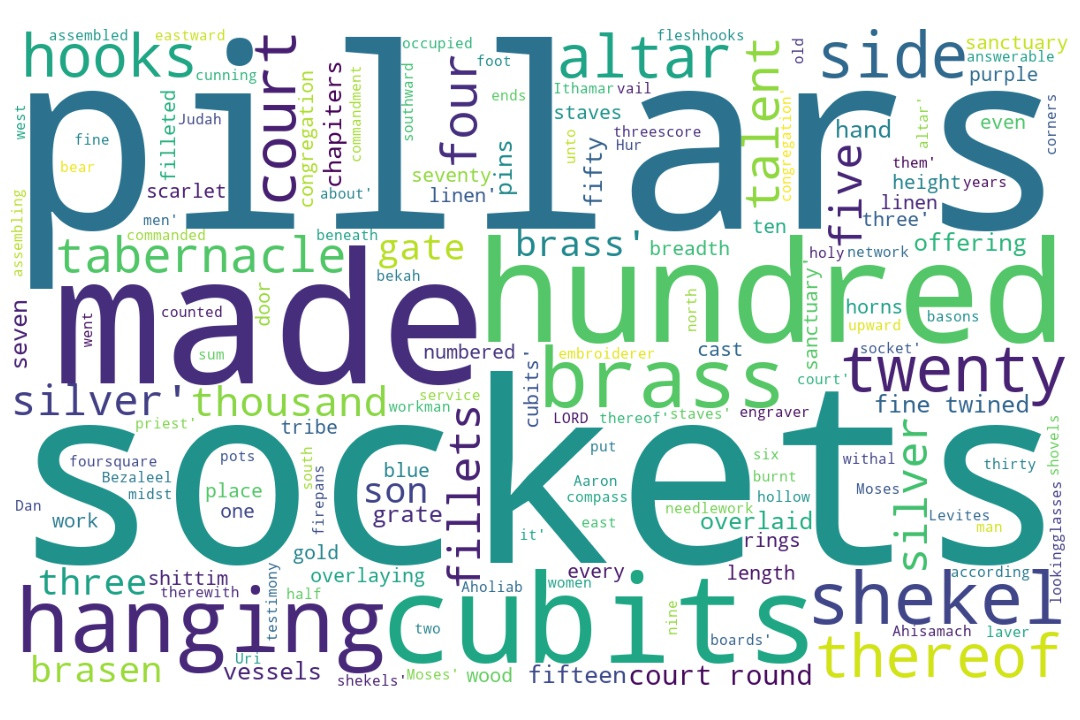
\includegraphics[width=\linewidth]{02OT-Exodus/Exodus38-WordCloud.jpg}
  \caption{Exodus 38 Word Cloud}
  \label{fig:Exodus 38 word Cloud}
\end{figure}


\marginpar{\scriptsize \centering \fcolorbox{bone}{lime}{\textbf{THE LAST PIECES}}\\ (Exodus 38:1--31) 
\begin{compactenum}[I.][8]
    \item A Place to \textbf{Burn} \index[scripture]{Exodus!Exo 38:01}(Exo 38:1)
    \item \textbf{Brass} Everywhere \index[scripture]{Exodus!Exo 38:02}\index[scripture]{Exodus!Exo 38:03}\index[scripture]{Exodus!Exo 38:05}\index[scripture]{Exodus!Exo 38:06}\index[scripture]{Exodus!Exo 38:08}\index[scripture]{Exodus!Exo 38:11}\index[scripture]{Exodus!Exo 38:17}\index[scripture]{Exodus!Exo 38:19}\index[scripture]{Exodus!Exo 38:20}\index[scripture]{Exodus!Exo 38:29}(Exo 38:2, 3, 5, 6, 8, 11, 17, 19, 20, 29)
    \item \textbf{Basons} \index[scripture]{Exodus!Exo 38:03}(Exo 38:3)  
    \item \textbf{Boards} \index[scripture]{Exodus!Exo 38:07}(Exo 38:7)  
    \item Somethings \textbf{Blue} \index[scripture]{Exodus!Exo 38:18}\index[scripture]{Exodus!Exo 38:23}(Exo 38:18, 23)  
    \item The \textbf{Book-keeping} \index[scripture]{Exodus!Exo 38:24--28}(Exo 38:24--28)  
\end{compactenum} }




\footnote{\textcolor[cmyk]{0.99998,1,0,0}{\hyperlink{TOC}{Return to end of Table of Contents.}}}\footnote{\href{https://audiobible.com/bible/exodus_38.html}{\textcolor[cmyk]{0.99998,1,0,0}{Exodus 38 Audio}}}\textcolor[cmyk]{0.99998,1,0,0}{And he made the \fcolorbox{bone}{lime}{altar of burnt offering} \emph{of} shittim wood: five cubits \emph{was} the length thereof, and five cubits the breadth thereof; \emph{it} \emph{was} foursquare; and three cubits the height thereof.}
[2] \textcolor[cmyk]{0.99998,1,0,0}{And he made the horns thereof on the four corners of it; the horns thereof were of the same: and he overlaid it with \fcolorbox{bone}{lime}{brass}.}
[3] \textcolor[cmyk]{0.99998,1,0,0}{And he made all the vessels of the altar, the pots, and the shovels, and the \fcolorbox{bone}{lime}{basons}, \emph{and} the fleshhooks, and the firepans: all the vessels thereof made he \emph{of} brass.}
[4] \textcolor[cmyk]{0.99998,1,0,0}{And he made for the altar a brasen grate of network under the compass thereof beneath unto the midst of it.}
[5] \textcolor[cmyk]{0.99998,1,0,0}{And he cast four rings for the four ends of the grate of brass, \emph{to} \emph{be} places for the staves.}
[6] \textcolor[cmyk]{0.99998,1,0,0}{And he made the staves \emph{of} shittim wood, and overlaid them with brass.}
[7] \textcolor[cmyk]{0.99998,1,0,0}{And he put the staves into the rings on the sides of the altar, to bear it withal; he made the altar hollow with \fcolorbox{bone}{lime}{boards}.}\\
\\
\P \textcolor[cmyk]{0.99998,1,0,0}{And he made the laver \emph{of} brass, and the foot of it \emph{of} brass, of the lookingglasses of \emph{the} \emph{women} assembling, which assembled \emph{at} the door of the tabernacle of the congregation.}\\
\\
\P \textcolor[cmyk]{0.99998,1,0,0}{And he made the court: on the south side southward the hangings of the court \fcolorbox{bone}{bone}{\emph{were}} \emph{of} fine twined linen, an hundred cubits:}
[10] \textcolor[cmyk]{0.99998,1,0,0}{Their \fcolorbox{bone}{bone}{pillars} \fcolorbox{bone}{bone}{\emph{were}} twenty, and their brasen \fcolorbox{bone}{bone}{sockets} twenty; the hooks of the \fcolorbox{bone}{bone}{pillars} and their fillets \fcolorbox{bone}{bone}{\emph{were}} \emph{of} silver.}
[11] \textcolor[cmyk]{0.99998,1,0,0}{And for the north side \emph{the} \emph{hangings} \fcolorbox{bone}{bone}{\emph{were}} an hundred cubits, their \fcolorbox{bone}{bone}{pillars} \fcolorbox{bone}{bone}{\emph{were}} twenty, and their \fcolorbox{bone}{bone}{sockets} of brass twenty; the hooks of the \fcolorbox{bone}{bone}{pillars} and their fillets \emph{of} silver.}
[12] \textcolor[cmyk]{0.99998,1,0,0}{And for the west side \fcolorbox{bone}{bone}{\emph{were}} hangings of fifty cubits, their \fcolorbox{bone}{bone}{pillars} ten, and their \fcolorbox{bone}{bone}{sockets} ten; the hooks of the \fcolorbox{bone}{bone}{pillars} and their fillets \emph{of} silver.}
[13] \textcolor[cmyk]{0.99998,1,0,0}{And for the east side eastward fifty cubits.}
[14] \textcolor[cmyk]{0.99998,1,0,0}{The hangings of the one side \emph{of} \emph{the} \emph{gate} \fcolorbox{bone}{bone}{\emph{were}} fifteen cubits; their \fcolorbox{bone}{bone}{pillars} three, and their \fcolorbox{bone}{bone}{sockets} three.}
[15] \textcolor[cmyk]{0.99998,1,0,0}{And for the other side of the court gate, on this hand and that hand, \fcolorbox{bone}{bone}{\emph{were}} hangings of fifteen cubits; their \fcolorbox{bone}{bone}{pillars} three, and their \fcolorbox{bone}{bone}{sockets} three.}
[16] \textcolor[cmyk]{0.99998,1,0,0}{All the hangings of the court round about \fcolorbox{bone}{bone}{\emph{were}} of fine twined linen.}
[17] \textcolor[cmyk]{0.99998,1,0,0}{And the \fcolorbox{bone}{bone}{sockets} for the \fcolorbox{bone}{bone}{pillars} \fcolorbox{bone}{bone}{\emph{were}} \emph{of} brass; the hooks of the \fcolorbox{bone}{bone}{pillars} and their fillets \emph{of} silver; and the overlaying of their chapiters \emph{of} silver; and all the \fcolorbox{bone}{bone}{pillars} of the court \fcolorbox{bone}{bone}{\emph{were}} filleted with silver.}
[18] \textcolor[cmyk]{0.99998,1,0,0}{And the hanging for the gate of the court \emph{was} needlework, \emph{of} \fcolorbox{bone}{lime}{blue}, and purple, and scarlet, and fine twined linen: and twenty cubits \emph{was} the length, and the height in the breadth \emph{was} five cubits, answerable to the hangings of the court.}
[19] \textcolor[cmyk]{0.99998,1,0,0}{And their \fcolorbox{bone}{bone}{pillars} \fcolorbox{bone}{bone}{\emph{were}} four, and their \fcolorbox{bone}{bone}{sockets} \emph{of} brass four; their hooks \emph{of} silver, and the overlaying of their chapiters and their fillets \emph{of} silver.}
[20] \textcolor[cmyk]{0.99998,1,0,0}{And all the pins of the tabernacle, and of the court round about, \fcolorbox{bone}{bone}{\emph{were}} \emph{of} brass.}\\
\\
\P \textcolor[cmyk]{0.99998,1,0,0}{This is the sum of the tabernacle, \emph{even} of the tabernacle of testimony, as it was counted, according to the commandment of Moses, \emph{for} the service of the Levites, by the hand of Ithamar, son to Aaron the priest.}
[22] \textcolor[cmyk]{0.99998,1,0,0}{And Bezaleel the son of Uri, the son of Hur, of the tribe of Judah, made all that the LORD commanded Moses.}
[23] \textcolor[cmyk]{0.99998,1,0,0}{And with him \emph{was} Aholiab, son of Ahisamach, of the tribe of Dan, an engraver, and a cunning workman, and an embroiderer in blue, and in purple, and in scarlet, and fine linen.}
[24] \textcolor[cmyk]{0.99998,1,0,0}{All the gold that was occupied for the work in all the work of the holy \emph{place}, even the gold of the offering, was twenty and nine talents, and seven hundred and thirty shekels, after the shekel of the sanctuary.}
[25] \textcolor[cmyk]{0.99998,1,0,0}{And the silver of them that were \fcolorbox{bone}{lime}{numbered} of the congregation \emph{was} an hundred talents, and a thousand seven hundred and threescore and fifteen shekels, after the shekel of the sanctuary:}
[26] \textcolor[cmyk]{0.99998,1,0,0}{A bekah for every man, \emph{that} \emph{is}, half a shekel, after the shekel of the sanctuary, for every one that went to be numbered, from twenty years old and upward, for six hundred thousand and three thousand and five hundred and fifty \emph{men}.}
[27] \textcolor[cmyk]{0.99998,1,0,0}{And of the hundred talents of silver were cast the \fcolorbox{bone}{bone}{sockets} of the sanctuary, and the \fcolorbox{bone}{bone}{sockets} of the vail; an hundred \fcolorbox{bone}{bone}{sockets} of the hundred talents, a talent for a socket.}
[28] \textcolor[cmyk]{0.99998,1,0,0}{And of the thousand seven hundred seventy and five shekels he made hooks for the \fcolorbox{bone}{bone}{pillars}, and overlaid their chapiters, and filleted them.}
[29] \textcolor[cmyk]{0.99998,1,0,0}{And the brass of the offering \emph{was} seventy talents, and two thousand and four hundred shekels.}
[30] \textcolor[cmyk]{0.99998,1,0,0}{And therewith he made the \fcolorbox{bone}{bone}{sockets} to the door of the tabernacle of the congregation, and the brasen altar, and the brasen grate for it, and all the vessels of the altar,}
[31] \textcolor[cmyk]{0.99998,1,0,0}{And the \fcolorbox{bone}{bone}{sockets} of the court round about, and the \fcolorbox{bone}{bone}{sockets} of the court gate, and all the pins of the tabernacle, and all the pins of the court round about.}
\index[NWIV]{32!Exodus!Exo 38:1}\index[AWIP]{And!Exodus!Exo 38:1}\index[AWIP]{he!Exodus!Exo 38:1}\index[AWIP]{made!Exodus!Exo 38:1}\index[AWIP]{the!Exodus!Exo 38:1}\index[AWIP]{the!Exodus!Exo 38:1 (2)}\index[AWIP]{the!Exodus!Exo 38:1 (3)}\index[AWIP]{the!Exodus!Exo 38:1 (4)}\index[AWIP]{altar!Exodus!Exo 38:1}\index[AWIP]{of!Exodus!Exo 38:1}\index[AWIP]{burnt!Exodus!Exo 38:1}\index[AWIP]{offering!Exodus!Exo 38:1}\index[AWIP]{\emph{of}!Exodus!Exo 38:1}\index[AWIP]{shittim!Exodus!Exo 38:1}\index[AWIP]{wood!Exodus!Exo 38:1}\index[AWIP]{five!Exodus!Exo 38:1}\index[AWIP]{five!Exodus!Exo 38:1 (2)}\index[AWIP]{cubits!Exodus!Exo 38:1}\index[AWIP]{cubits!Exodus!Exo 38:1 (2)}\index[AWIP]{cubits!Exodus!Exo 38:1 (3)}\index[AWIP]{\emph{was}!Exodus!Exo 38:1}\index[AWIP]{\emph{was}!Exodus!Exo 38:1 (2)}\index[AWIP]{length!Exodus!Exo 38:1}\index[AWIP]{thereof!Exodus!Exo 38:1}\index[AWIP]{thereof!Exodus!Exo 38:1 (2)}\index[AWIP]{thereof!Exodus!Exo 38:1 (3)}\index[AWIP]{and!Exodus!Exo 38:1}\index[AWIP]{and!Exodus!Exo 38:1 (2)}\index[AWIP]{breadth!Exodus!Exo 38:1}\index[AWIP]{\emph{it}!Exodus!Exo 38:1}\index[AWIP]{foursquare!Exodus!Exo 38:1}\index[AWIP]{three!Exodus!Exo 38:1}\index[AWIP]{height!Exodus!Exo 38:1}\index[AWIP]{\emph{of}!Exodus!Exo 38:1}\index[AWIP]{\emph{was}!Exodus!Exo 38:1}\index[AWIP]{\emph{was}!Exodus!Exo 38:1 (2)}\index[AWIP]{\emph{it}!Exodus!Exo 38:1}

\index[NWIV]{25!Exodus!Exo 38:2}\index[AWIP]{And!Exodus!Exo 38:2}\index[AWIP]{he!Exodus!Exo 38:2}\index[AWIP]{he!Exodus!Exo 38:2 (2)}\index[AWIP]{made!Exodus!Exo 38:2}\index[AWIP]{the!Exodus!Exo 38:2}\index[AWIP]{the!Exodus!Exo 38:2 (2)}\index[AWIP]{the!Exodus!Exo 38:2 (3)}\index[AWIP]{the!Exodus!Exo 38:2 (4)}\index[AWIP]{horns!Exodus!Exo 38:2}\index[AWIP]{horns!Exodus!Exo 38:2 (2)}\index[AWIP]{thereof!Exodus!Exo 38:2}\index[AWIP]{thereof!Exodus!Exo 38:2 (2)}\index[AWIP]{on!Exodus!Exo 38:2}\index[AWIP]{four!Exodus!Exo 38:2}\index[AWIP]{corners!Exodus!Exo 38:2}\index[AWIP]{of!Exodus!Exo 38:2}\index[AWIP]{of!Exodus!Exo 38:2 (2)}\index[AWIP]{it!Exodus!Exo 38:2}\index[AWIP]{it!Exodus!Exo 38:2 (2)}\index[AWIP]{were!Exodus!Exo 38:2}\index[AWIP]{same!Exodus!Exo 38:2}\index[AWIP]{and!Exodus!Exo 38:2}\index[AWIP]{overlaid!Exodus!Exo 38:2}\index[AWIP]{with!Exodus!Exo 38:2}\index[AWIP]{brass!Exodus!Exo 38:2}

\index[NWIV]{31!Exodus!Exo 38:3}\index[AWIP]{And!Exodus!Exo 38:3}\index[AWIP]{he!Exodus!Exo 38:3}\index[AWIP]{he!Exodus!Exo 38:3 (2)}\index[AWIP]{made!Exodus!Exo 38:3}\index[AWIP]{made!Exodus!Exo 38:3 (2)}\index[AWIP]{all!Exodus!Exo 38:3}\index[AWIP]{all!Exodus!Exo 38:3 (2)}\index[AWIP]{the!Exodus!Exo 38:3}\index[AWIP]{the!Exodus!Exo 38:3 (2)}\index[AWIP]{the!Exodus!Exo 38:3 (3)}\index[AWIP]{the!Exodus!Exo 38:3 (4)}\index[AWIP]{the!Exodus!Exo 38:3 (5)}\index[AWIP]{the!Exodus!Exo 38:3 (6)}\index[AWIP]{the!Exodus!Exo 38:3 (7)}\index[AWIP]{the!Exodus!Exo 38:3 (8)}\index[AWIP]{vessels!Exodus!Exo 38:3}\index[AWIP]{vessels!Exodus!Exo 38:3 (2)}\index[AWIP]{of!Exodus!Exo 38:3}\index[AWIP]{altar!Exodus!Exo 38:3}\index[AWIP]{pots!Exodus!Exo 38:3}\index[AWIP]{and!Exodus!Exo 38:3}\index[AWIP]{and!Exodus!Exo 38:3 (2)}\index[AWIP]{and!Exodus!Exo 38:3 (3)}\index[AWIP]{shovels!Exodus!Exo 38:3}\index[AWIP]{basons!Exodus!Exo 38:3}\index[AWIP]{\emph{and}!Exodus!Exo 38:3}\index[AWIP]{fleshhooks!Exodus!Exo 38:3}\index[AWIP]{firepans!Exodus!Exo 38:3}\index[AWIP]{thereof!Exodus!Exo 38:3}\index[AWIP]{\emph{of}!Exodus!Exo 38:3}\index[AWIP]{brass!Exodus!Exo 38:3}\index[AWIP]{\emph{and}!Exodus!Exo 38:3}\index[AWIP]{\emph{of}!Exodus!Exo 38:3}

\index[NWIV]{21!Exodus!Exo 38:4}\index[AWIP]{And!Exodus!Exo 38:4}\index[AWIP]{he!Exodus!Exo 38:4}\index[AWIP]{made!Exodus!Exo 38:4}\index[AWIP]{for!Exodus!Exo 38:4}\index[AWIP]{the!Exodus!Exo 38:4}\index[AWIP]{the!Exodus!Exo 38:4 (2)}\index[AWIP]{the!Exodus!Exo 38:4 (3)}\index[AWIP]{altar!Exodus!Exo 38:4}\index[AWIP]{a!Exodus!Exo 38:4}\index[AWIP]{brasen!Exodus!Exo 38:4}\index[AWIP]{grate!Exodus!Exo 38:4}\index[AWIP]{of!Exodus!Exo 38:4}\index[AWIP]{of!Exodus!Exo 38:4 (2)}\index[AWIP]{network!Exodus!Exo 38:4}\index[AWIP]{under!Exodus!Exo 38:4}\index[AWIP]{compass!Exodus!Exo 38:4}\index[AWIP]{thereof!Exodus!Exo 38:4}\index[AWIP]{beneath!Exodus!Exo 38:4}\index[AWIP]{unto!Exodus!Exo 38:4}\index[AWIP]{midst!Exodus!Exo 38:4}\index[AWIP]{it!Exodus!Exo 38:4}

\index[NWIV]{20!Exodus!Exo 38:5}\index[AWIP]{And!Exodus!Exo 38:5}\index[AWIP]{he!Exodus!Exo 38:5}\index[AWIP]{cast!Exodus!Exo 38:5}\index[AWIP]{four!Exodus!Exo 38:5}\index[AWIP]{four!Exodus!Exo 38:5 (2)}\index[AWIP]{rings!Exodus!Exo 38:5}\index[AWIP]{for!Exodus!Exo 38:5}\index[AWIP]{for!Exodus!Exo 38:5 (2)}\index[AWIP]{the!Exodus!Exo 38:5}\index[AWIP]{the!Exodus!Exo 38:5 (2)}\index[AWIP]{the!Exodus!Exo 38:5 (3)}\index[AWIP]{ends!Exodus!Exo 38:5}\index[AWIP]{of!Exodus!Exo 38:5}\index[AWIP]{of!Exodus!Exo 38:5 (2)}\index[AWIP]{grate!Exodus!Exo 38:5}\index[AWIP]{brass!Exodus!Exo 38:5}\index[AWIP]{\emph{to}!Exodus!Exo 38:5}\index[AWIP]{\emph{be}!Exodus!Exo 38:5}\index[AWIP]{places!Exodus!Exo 38:5}\index[AWIP]{staves!Exodus!Exo 38:5}\index[AWIP]{\emph{to}!Exodus!Exo 38:5}\index[AWIP]{\emph{be}!Exodus!Exo 38:5}

\index[NWIV]{13!Exodus!Exo 38:6}\index[AWIP]{And!Exodus!Exo 38:6}\index[AWIP]{he!Exodus!Exo 38:6}\index[AWIP]{made!Exodus!Exo 38:6}\index[AWIP]{the!Exodus!Exo 38:6}\index[AWIP]{staves!Exodus!Exo 38:6}\index[AWIP]{\emph{of}!Exodus!Exo 38:6}\index[AWIP]{shittim!Exodus!Exo 38:6}\index[AWIP]{wood!Exodus!Exo 38:6}\index[AWIP]{and!Exodus!Exo 38:6}\index[AWIP]{overlaid!Exodus!Exo 38:6}\index[AWIP]{them!Exodus!Exo 38:6}\index[AWIP]{with!Exodus!Exo 38:6}\index[AWIP]{brass!Exodus!Exo 38:6}\index[AWIP]{\emph{of}!Exodus!Exo 38:6}

\index[NWIV]{25!Exodus!Exo 38:7}\index[AWIP]{And!Exodus!Exo 38:7}\index[AWIP]{he!Exodus!Exo 38:7}\index[AWIP]{he!Exodus!Exo 38:7 (2)}\index[AWIP]{put!Exodus!Exo 38:7}\index[AWIP]{the!Exodus!Exo 38:7}\index[AWIP]{the!Exodus!Exo 38:7 (2)}\index[AWIP]{the!Exodus!Exo 38:7 (3)}\index[AWIP]{the!Exodus!Exo 38:7 (4)}\index[AWIP]{the!Exodus!Exo 38:7 (5)}\index[AWIP]{staves!Exodus!Exo 38:7}\index[AWIP]{into!Exodus!Exo 38:7}\index[AWIP]{rings!Exodus!Exo 38:7}\index[AWIP]{on!Exodus!Exo 38:7}\index[AWIP]{sides!Exodus!Exo 38:7}\index[AWIP]{of!Exodus!Exo 38:7}\index[AWIP]{altar!Exodus!Exo 38:7}\index[AWIP]{altar!Exodus!Exo 38:7 (2)}\index[AWIP]{to!Exodus!Exo 38:7}\index[AWIP]{bear!Exodus!Exo 38:7}\index[AWIP]{it!Exodus!Exo 38:7}\index[AWIP]{withal!Exodus!Exo 38:7}\index[AWIP]{made!Exodus!Exo 38:7}\index[AWIP]{hollow!Exodus!Exo 38:7}\index[AWIP]{with!Exodus!Exo 38:7}\index[AWIP]{boards!Exodus!Exo 38:7}

\index[NWIV]{32!Exodus!Exo 38:8}\index[AWIP]{And!Exodus!Exo 38:8}\index[AWIP]{he!Exodus!Exo 38:8}\index[AWIP]{made!Exodus!Exo 38:8}\index[AWIP]{the!Exodus!Exo 38:8}\index[AWIP]{the!Exodus!Exo 38:8 (2)}\index[AWIP]{the!Exodus!Exo 38:8 (3)}\index[AWIP]{the!Exodus!Exo 38:8 (4)}\index[AWIP]{the!Exodus!Exo 38:8 (5)}\index[AWIP]{the!Exodus!Exo 38:8 (6)}\index[AWIP]{laver!Exodus!Exo 38:8}\index[AWIP]{\emph{of}!Exodus!Exo 38:8}\index[AWIP]{\emph{of}!Exodus!Exo 38:8 (2)}\index[AWIP]{brass!Exodus!Exo 38:8}\index[AWIP]{brass!Exodus!Exo 38:8 (2)}\index[AWIP]{and!Exodus!Exo 38:8}\index[AWIP]{foot!Exodus!Exo 38:8}\index[AWIP]{of!Exodus!Exo 38:8}\index[AWIP]{of!Exodus!Exo 38:8 (2)}\index[AWIP]{of!Exodus!Exo 38:8 (3)}\index[AWIP]{of!Exodus!Exo 38:8 (4)}\index[AWIP]{of!Exodus!Exo 38:8 (5)}\index[AWIP]{it!Exodus!Exo 38:8}\index[AWIP]{lookingglasses!Exodus!Exo 38:8}\index[AWIP]{\emph{the}!Exodus!Exo 38:8}\index[AWIP]{\emph{women}!Exodus!Exo 38:8}\index[AWIP]{assembling!Exodus!Exo 38:8}\index[AWIP]{which!Exodus!Exo 38:8}\index[AWIP]{assembled!Exodus!Exo 38:8}\index[AWIP]{\emph{at}!Exodus!Exo 38:8}\index[AWIP]{door!Exodus!Exo 38:8}\index[AWIP]{tabernacle!Exodus!Exo 38:8}\index[AWIP]{congregation!Exodus!Exo 38:8}\index[AWIP]{\emph{of}!Exodus!Exo 38:8}\index[AWIP]{\emph{of}!Exodus!Exo 38:8 (2)}\index[AWIP]{\emph{the}!Exodus!Exo 38:8}\index[AWIP]{\emph{women}!Exodus!Exo 38:8}\index[AWIP]{\emph{at}!Exodus!Exo 38:8}

\index[NWIV]{23!Exodus!Exo 38:9}\index[AWIP]{And!Exodus!Exo 38:9}\index[AWIP]{he!Exodus!Exo 38:9}\index[AWIP]{made!Exodus!Exo 38:9}\index[AWIP]{the!Exodus!Exo 38:9}\index[AWIP]{the!Exodus!Exo 38:9 (2)}\index[AWIP]{the!Exodus!Exo 38:9 (3)}\index[AWIP]{the!Exodus!Exo 38:9 (4)}\index[AWIP]{court!Exodus!Exo 38:9}\index[AWIP]{court!Exodus!Exo 38:9 (2)}\index[AWIP]{on!Exodus!Exo 38:9}\index[AWIP]{south!Exodus!Exo 38:9}\index[AWIP]{side!Exodus!Exo 38:9}\index[AWIP]{southward!Exodus!Exo 38:9}\index[AWIP]{hangings!Exodus!Exo 38:9}\index[AWIP]{of!Exodus!Exo 38:9}\index[AWIP]{\emph{were}!Exodus!Exo 38:9}\index[AWIP]{\emph{of}!Exodus!Exo 38:9}\index[AWIP]{fine!Exodus!Exo 38:9}\index[AWIP]{twined!Exodus!Exo 38:9}\index[AWIP]{linen!Exodus!Exo 38:9}\index[AWIP]{an!Exodus!Exo 38:9}\index[AWIP]{hundred!Exodus!Exo 38:9}\index[AWIP]{cubits!Exodus!Exo 38:9}\index[AWIP]{\emph{were}!Exodus!Exo 38:9}\index[AWIP]{\emph{of}!Exodus!Exo 38:9}

\index[NWIV]{20!Exodus!Exo 38:10}\index[AWIP]{Their!Exodus!Exo 38:10}\index[AWIP]{pillars!Exodus!Exo 38:10}\index[AWIP]{pillars!Exodus!Exo 38:10 (2)}\index[AWIP]{\emph{were}!Exodus!Exo 38:10}\index[AWIP]{\emph{were}!Exodus!Exo 38:10 (2)}\index[AWIP]{twenty!Exodus!Exo 38:10}\index[AWIP]{twenty!Exodus!Exo 38:10 (2)}\index[AWIP]{and!Exodus!Exo 38:10}\index[AWIP]{and!Exodus!Exo 38:10 (2)}\index[AWIP]{their!Exodus!Exo 38:10}\index[AWIP]{their!Exodus!Exo 38:10 (2)}\index[AWIP]{brasen!Exodus!Exo 38:10}\index[AWIP]{sockets!Exodus!Exo 38:10}\index[AWIP]{the!Exodus!Exo 38:10}\index[AWIP]{the!Exodus!Exo 38:10 (2)}\index[AWIP]{hooks!Exodus!Exo 38:10}\index[AWIP]{of!Exodus!Exo 38:10}\index[AWIP]{fillets!Exodus!Exo 38:10}\index[AWIP]{\emph{of}!Exodus!Exo 38:10}\index[AWIP]{silver!Exodus!Exo 38:10}\index[AWIP]{\emph{were}!Exodus!Exo 38:10}\index[AWIP]{\emph{were}!Exodus!Exo 38:10 (2)}\index[AWIP]{\emph{of}!Exodus!Exo 38:10}

\index[NWIV]{31!Exodus!Exo 38:11}\index[AWIP]{And!Exodus!Exo 38:11}\index[AWIP]{for!Exodus!Exo 38:11}\index[AWIP]{the!Exodus!Exo 38:11}\index[AWIP]{the!Exodus!Exo 38:11 (2)}\index[AWIP]{the!Exodus!Exo 38:11 (3)}\index[AWIP]{north!Exodus!Exo 38:11}\index[AWIP]{side!Exodus!Exo 38:11}\index[AWIP]{\emph{the}!Exodus!Exo 38:11}\index[AWIP]{\emph{hangings}!Exodus!Exo 38:11}\index[AWIP]{\emph{were}!Exodus!Exo 38:11}\index[AWIP]{\emph{were}!Exodus!Exo 38:11 (2)}\index[AWIP]{an!Exodus!Exo 38:11}\index[AWIP]{hundred!Exodus!Exo 38:11}\index[AWIP]{cubits!Exodus!Exo 38:11}\index[AWIP]{their!Exodus!Exo 38:11}\index[AWIP]{their!Exodus!Exo 38:11 (2)}\index[AWIP]{their!Exodus!Exo 38:11 (3)}\index[AWIP]{pillars!Exodus!Exo 38:11}\index[AWIP]{pillars!Exodus!Exo 38:11 (2)}\index[AWIP]{twenty!Exodus!Exo 38:11}\index[AWIP]{twenty!Exodus!Exo 38:11 (2)}\index[AWIP]{and!Exodus!Exo 38:11}\index[AWIP]{and!Exodus!Exo 38:11 (2)}\index[AWIP]{sockets!Exodus!Exo 38:11}\index[AWIP]{of!Exodus!Exo 38:11}\index[AWIP]{of!Exodus!Exo 38:11 (2)}\index[AWIP]{brass!Exodus!Exo 38:11}\index[AWIP]{hooks!Exodus!Exo 38:11}\index[AWIP]{fillets!Exodus!Exo 38:11}\index[AWIP]{\emph{of}!Exodus!Exo 38:11}\index[AWIP]{silver!Exodus!Exo 38:11}\index[AWIP]{\emph{the}!Exodus!Exo 38:11}\index[AWIP]{\emph{hangings}!Exodus!Exo 38:11}\index[AWIP]{\emph{were}!Exodus!Exo 38:11}\index[AWIP]{\emph{were}!Exodus!Exo 38:11 (2)}\index[AWIP]{\emph{of}!Exodus!Exo 38:11}

\index[NWIV]{27!Exodus!Exo 38:12}\index[AWIP]{And!Exodus!Exo 38:12}\index[AWIP]{for!Exodus!Exo 38:12}\index[AWIP]{the!Exodus!Exo 38:12}\index[AWIP]{the!Exodus!Exo 38:12 (2)}\index[AWIP]{the!Exodus!Exo 38:12 (3)}\index[AWIP]{west!Exodus!Exo 38:12}\index[AWIP]{side!Exodus!Exo 38:12}\index[AWIP]{\emph{were}!Exodus!Exo 38:12}\index[AWIP]{hangings!Exodus!Exo 38:12}\index[AWIP]{of!Exodus!Exo 38:12}\index[AWIP]{of!Exodus!Exo 38:12 (2)}\index[AWIP]{fifty!Exodus!Exo 38:12}\index[AWIP]{cubits!Exodus!Exo 38:12}\index[AWIP]{their!Exodus!Exo 38:12}\index[AWIP]{their!Exodus!Exo 38:12 (2)}\index[AWIP]{their!Exodus!Exo 38:12 (3)}\index[AWIP]{pillars!Exodus!Exo 38:12}\index[AWIP]{pillars!Exodus!Exo 38:12 (2)}\index[AWIP]{ten!Exodus!Exo 38:12}\index[AWIP]{ten!Exodus!Exo 38:12 (2)}\index[AWIP]{and!Exodus!Exo 38:12}\index[AWIP]{and!Exodus!Exo 38:12 (2)}\index[AWIP]{sockets!Exodus!Exo 38:12}\index[AWIP]{hooks!Exodus!Exo 38:12}\index[AWIP]{fillets!Exodus!Exo 38:12}\index[AWIP]{\emph{of}!Exodus!Exo 38:12}\index[AWIP]{silver!Exodus!Exo 38:12}\index[AWIP]{\emph{were}!Exodus!Exo 38:12}\index[AWIP]{\emph{of}!Exodus!Exo 38:12}

\index[NWIV]{8!Exodus!Exo 38:13}\index[AWIP]{And!Exodus!Exo 38:13}\index[AWIP]{for!Exodus!Exo 38:13}\index[AWIP]{the!Exodus!Exo 38:13}\index[AWIP]{east!Exodus!Exo 38:13}\index[AWIP]{side!Exodus!Exo 38:13}\index[AWIP]{eastward!Exodus!Exo 38:13}\index[AWIP]{fifty!Exodus!Exo 38:13}\index[AWIP]{cubits!Exodus!Exo 38:13}

\index[NWIV]{19!Exodus!Exo 38:14}\index[AWIP]{The!Exodus!Exo 38:14}\index[AWIP]{hangings!Exodus!Exo 38:14}\index[AWIP]{of!Exodus!Exo 38:14}\index[AWIP]{the!Exodus!Exo 38:14}\index[AWIP]{one!Exodus!Exo 38:14}\index[AWIP]{side!Exodus!Exo 38:14}\index[AWIP]{\emph{of}!Exodus!Exo 38:14}\index[AWIP]{\emph{the}!Exodus!Exo 38:14}\index[AWIP]{\emph{gate}!Exodus!Exo 38:14}\index[AWIP]{\emph{were}!Exodus!Exo 38:14}\index[AWIP]{fifteen!Exodus!Exo 38:14}\index[AWIP]{cubits!Exodus!Exo 38:14}\index[AWIP]{their!Exodus!Exo 38:14}\index[AWIP]{their!Exodus!Exo 38:14 (2)}\index[AWIP]{pillars!Exodus!Exo 38:14}\index[AWIP]{three!Exodus!Exo 38:14}\index[AWIP]{three!Exodus!Exo 38:14 (2)}\index[AWIP]{and!Exodus!Exo 38:14}\index[AWIP]{sockets!Exodus!Exo 38:14}\index[AWIP]{\emph{of}!Exodus!Exo 38:14}\index[AWIP]{\emph{the}!Exodus!Exo 38:14}\index[AWIP]{\emph{gate}!Exodus!Exo 38:14}\index[AWIP]{\emph{were}!Exodus!Exo 38:14}

\index[NWIV]{27!Exodus!Exo 38:15}\index[AWIP]{And!Exodus!Exo 38:15}\index[AWIP]{for!Exodus!Exo 38:15}\index[AWIP]{the!Exodus!Exo 38:15}\index[AWIP]{the!Exodus!Exo 38:15 (2)}\index[AWIP]{other!Exodus!Exo 38:15}\index[AWIP]{side!Exodus!Exo 38:15}\index[AWIP]{of!Exodus!Exo 38:15}\index[AWIP]{of!Exodus!Exo 38:15 (2)}\index[AWIP]{court!Exodus!Exo 38:15}\index[AWIP]{gate!Exodus!Exo 38:15}\index[AWIP]{on!Exodus!Exo 38:15}\index[AWIP]{this!Exodus!Exo 38:15}\index[AWIP]{hand!Exodus!Exo 38:15}\index[AWIP]{hand!Exodus!Exo 38:15 (2)}\index[AWIP]{and!Exodus!Exo 38:15}\index[AWIP]{and!Exodus!Exo 38:15 (2)}\index[AWIP]{that!Exodus!Exo 38:15}\index[AWIP]{\emph{were}!Exodus!Exo 38:15}\index[AWIP]{hangings!Exodus!Exo 38:15}\index[AWIP]{fifteen!Exodus!Exo 38:15}\index[AWIP]{cubits!Exodus!Exo 38:15}\index[AWIP]{their!Exodus!Exo 38:15}\index[AWIP]{their!Exodus!Exo 38:15 (2)}\index[AWIP]{pillars!Exodus!Exo 38:15}\index[AWIP]{three!Exodus!Exo 38:15}\index[AWIP]{three!Exodus!Exo 38:15 (2)}\index[AWIP]{sockets!Exodus!Exo 38:15}\index[AWIP]{\emph{were}!Exodus!Exo 38:15}

\index[NWIV]{13!Exodus!Exo 38:16}\index[AWIP]{All!Exodus!Exo 38:16}\index[AWIP]{the!Exodus!Exo 38:16}\index[AWIP]{the!Exodus!Exo 38:16 (2)}\index[AWIP]{hangings!Exodus!Exo 38:16}\index[AWIP]{of!Exodus!Exo 38:16}\index[AWIP]{of!Exodus!Exo 38:16 (2)}\index[AWIP]{court!Exodus!Exo 38:16}\index[AWIP]{round!Exodus!Exo 38:16}\index[AWIP]{about!Exodus!Exo 38:16}\index[AWIP]{\emph{were}!Exodus!Exo 38:16}\index[AWIP]{fine!Exodus!Exo 38:16}\index[AWIP]{twined!Exodus!Exo 38:16}\index[AWIP]{linen!Exodus!Exo 38:16}\index[AWIP]{\emph{were}!Exodus!Exo 38:16}

\index[NWIV]{38!Exodus!Exo 38:17}\index[AWIP]{And!Exodus!Exo 38:17}\index[AWIP]{the!Exodus!Exo 38:17}\index[AWIP]{the!Exodus!Exo 38:17 (2)}\index[AWIP]{the!Exodus!Exo 38:17 (3)}\index[AWIP]{the!Exodus!Exo 38:17 (4)}\index[AWIP]{the!Exodus!Exo 38:17 (5)}\index[AWIP]{the!Exodus!Exo 38:17 (6)}\index[AWIP]{the!Exodus!Exo 38:17 (7)}\index[AWIP]{sockets!Exodus!Exo 38:17}\index[AWIP]{for!Exodus!Exo 38:17}\index[AWIP]{pillars!Exodus!Exo 38:17}\index[AWIP]{pillars!Exodus!Exo 38:17 (2)}\index[AWIP]{pillars!Exodus!Exo 38:17 (3)}\index[AWIP]{\emph{were}!Exodus!Exo 38:17}\index[AWIP]{\emph{were}!Exodus!Exo 38:17 (2)}\index[AWIP]{\emph{of}!Exodus!Exo 38:17}\index[AWIP]{\emph{of}!Exodus!Exo 38:17 (2)}\index[AWIP]{\emph{of}!Exodus!Exo 38:17 (3)}\index[AWIP]{brass!Exodus!Exo 38:17}\index[AWIP]{hooks!Exodus!Exo 38:17}\index[AWIP]{of!Exodus!Exo 38:17}\index[AWIP]{of!Exodus!Exo 38:17 (2)}\index[AWIP]{of!Exodus!Exo 38:17 (3)}\index[AWIP]{and!Exodus!Exo 38:17}\index[AWIP]{and!Exodus!Exo 38:17 (2)}\index[AWIP]{and!Exodus!Exo 38:17 (3)}\index[AWIP]{their!Exodus!Exo 38:17}\index[AWIP]{their!Exodus!Exo 38:17 (2)}\index[AWIP]{fillets!Exodus!Exo 38:17}\index[AWIP]{silver!Exodus!Exo 38:17}\index[AWIP]{silver!Exodus!Exo 38:17 (2)}\index[AWIP]{silver!Exodus!Exo 38:17 (3)}\index[AWIP]{overlaying!Exodus!Exo 38:17}\index[AWIP]{chapiters!Exodus!Exo 38:17}\index[AWIP]{all!Exodus!Exo 38:17}\index[AWIP]{court!Exodus!Exo 38:17}\index[AWIP]{filleted!Exodus!Exo 38:17}\index[AWIP]{with!Exodus!Exo 38:17}\index[AWIP]{\emph{were}!Exodus!Exo 38:17}\index[AWIP]{\emph{were}!Exodus!Exo 38:17 (2)}\index[AWIP]{\emph{of}!Exodus!Exo 38:17}\index[AWIP]{\emph{of}!Exodus!Exo 38:17 (2)}\index[AWIP]{\emph{of}!Exodus!Exo 38:17 (3)}

\index[NWIV]{43!Exodus!Exo 38:18}\index[AWIP]{And!Exodus!Exo 38:18}\index[AWIP]{the!Exodus!Exo 38:18}\index[AWIP]{the!Exodus!Exo 38:18 (2)}\index[AWIP]{the!Exodus!Exo 38:18 (3)}\index[AWIP]{the!Exodus!Exo 38:18 (4)}\index[AWIP]{the!Exodus!Exo 38:18 (5)}\index[AWIP]{the!Exodus!Exo 38:18 (6)}\index[AWIP]{the!Exodus!Exo 38:18 (7)}\index[AWIP]{the!Exodus!Exo 38:18 (8)}\index[AWIP]{hanging!Exodus!Exo 38:18}\index[AWIP]{for!Exodus!Exo 38:18}\index[AWIP]{gate!Exodus!Exo 38:18}\index[AWIP]{of!Exodus!Exo 38:18}\index[AWIP]{of!Exodus!Exo 38:18 (2)}\index[AWIP]{court!Exodus!Exo 38:18}\index[AWIP]{court!Exodus!Exo 38:18 (2)}\index[AWIP]{\emph{was}!Exodus!Exo 38:18}\index[AWIP]{\emph{was}!Exodus!Exo 38:18 (2)}\index[AWIP]{\emph{was}!Exodus!Exo 38:18 (3)}\index[AWIP]{needlework!Exodus!Exo 38:18}\index[AWIP]{\emph{of}!Exodus!Exo 38:18}\index[AWIP]{blue!Exodus!Exo 38:18}\index[AWIP]{and!Exodus!Exo 38:18}\index[AWIP]{and!Exodus!Exo 38:18 (2)}\index[AWIP]{and!Exodus!Exo 38:18 (3)}\index[AWIP]{and!Exodus!Exo 38:18 (4)}\index[AWIP]{and!Exodus!Exo 38:18 (5)}\index[AWIP]{purple!Exodus!Exo 38:18}\index[AWIP]{scarlet!Exodus!Exo 38:18}\index[AWIP]{fine!Exodus!Exo 38:18}\index[AWIP]{twined!Exodus!Exo 38:18}\index[AWIP]{linen!Exodus!Exo 38:18}\index[AWIP]{twenty!Exodus!Exo 38:18}\index[AWIP]{cubits!Exodus!Exo 38:18}\index[AWIP]{cubits!Exodus!Exo 38:18 (2)}\index[AWIP]{length!Exodus!Exo 38:18}\index[AWIP]{height!Exodus!Exo 38:18}\index[AWIP]{in!Exodus!Exo 38:18}\index[AWIP]{breadth!Exodus!Exo 38:18}\index[AWIP]{five!Exodus!Exo 38:18}\index[AWIP]{answerable!Exodus!Exo 38:18}\index[AWIP]{to!Exodus!Exo 38:18}\index[AWIP]{hangings!Exodus!Exo 38:18}\index[AWIP]{\emph{was}!Exodus!Exo 38:18}\index[AWIP]{\emph{was}!Exodus!Exo 38:18 (2)}\index[AWIP]{\emph{was}!Exodus!Exo 38:18 (3)}\index[AWIP]{\emph{of}!Exodus!Exo 38:18}

\index[NWIV]{26!Exodus!Exo 38:19}\index[AWIP]{And!Exodus!Exo 38:19}\index[AWIP]{their!Exodus!Exo 38:19}\index[AWIP]{their!Exodus!Exo 38:19 (2)}\index[AWIP]{their!Exodus!Exo 38:19 (3)}\index[AWIP]{their!Exodus!Exo 38:19 (4)}\index[AWIP]{their!Exodus!Exo 38:19 (5)}\index[AWIP]{pillars!Exodus!Exo 38:19}\index[AWIP]{\emph{were}!Exodus!Exo 38:19}\index[AWIP]{four!Exodus!Exo 38:19}\index[AWIP]{four!Exodus!Exo 38:19 (2)}\index[AWIP]{and!Exodus!Exo 38:19}\index[AWIP]{and!Exodus!Exo 38:19 (2)}\index[AWIP]{and!Exodus!Exo 38:19 (3)}\index[AWIP]{sockets!Exodus!Exo 38:19}\index[AWIP]{\emph{of}!Exodus!Exo 38:19}\index[AWIP]{\emph{of}!Exodus!Exo 38:19 (2)}\index[AWIP]{\emph{of}!Exodus!Exo 38:19 (3)}\index[AWIP]{brass!Exodus!Exo 38:19}\index[AWIP]{hooks!Exodus!Exo 38:19}\index[AWIP]{silver!Exodus!Exo 38:19}\index[AWIP]{silver!Exodus!Exo 38:19 (2)}\index[AWIP]{the!Exodus!Exo 38:19}\index[AWIP]{overlaying!Exodus!Exo 38:19}\index[AWIP]{of!Exodus!Exo 38:19}\index[AWIP]{chapiters!Exodus!Exo 38:19}\index[AWIP]{fillets!Exodus!Exo 38:19}\index[AWIP]{\emph{were}!Exodus!Exo 38:19}\index[AWIP]{\emph{of}!Exodus!Exo 38:19}\index[AWIP]{\emph{of}!Exodus!Exo 38:19 (2)}\index[AWIP]{\emph{of}!Exodus!Exo 38:19 (3)}

\index[NWIV]{16!Exodus!Exo 38:20}\index[AWIP]{And!Exodus!Exo 38:20}\index[AWIP]{all!Exodus!Exo 38:20}\index[AWIP]{the!Exodus!Exo 38:20}\index[AWIP]{the!Exodus!Exo 38:20 (2)}\index[AWIP]{the!Exodus!Exo 38:20 (3)}\index[AWIP]{pins!Exodus!Exo 38:20}\index[AWIP]{of!Exodus!Exo 38:20}\index[AWIP]{of!Exodus!Exo 38:20 (2)}\index[AWIP]{tabernacle!Exodus!Exo 38:20}\index[AWIP]{and!Exodus!Exo 38:20}\index[AWIP]{court!Exodus!Exo 38:20}\index[AWIP]{round!Exodus!Exo 38:20}\index[AWIP]{about!Exodus!Exo 38:20}\index[AWIP]{\emph{were}!Exodus!Exo 38:20}\index[AWIP]{\emph{of}!Exodus!Exo 38:20}\index[AWIP]{brass!Exodus!Exo 38:20}\index[AWIP]{\emph{were}!Exodus!Exo 38:20}\index[AWIP]{\emph{of}!Exodus!Exo 38:20}

\index[NWIV]{39!Exodus!Exo 38:21}\index[AWIP]{This!Exodus!Exo 38:21}\index[AWIP]{is!Exodus!Exo 38:21}\index[AWIP]{the!Exodus!Exo 38:21}\index[AWIP]{the!Exodus!Exo 38:21 (2)}\index[AWIP]{the!Exodus!Exo 38:21 (3)}\index[AWIP]{the!Exodus!Exo 38:21 (4)}\index[AWIP]{the!Exodus!Exo 38:21 (5)}\index[AWIP]{the!Exodus!Exo 38:21 (6)}\index[AWIP]{the!Exodus!Exo 38:21 (7)}\index[AWIP]{the!Exodus!Exo 38:21 (8)}\index[AWIP]{sum!Exodus!Exo 38:21}\index[AWIP]{of!Exodus!Exo 38:21}\index[AWIP]{of!Exodus!Exo 38:21 (2)}\index[AWIP]{of!Exodus!Exo 38:21 (3)}\index[AWIP]{of!Exodus!Exo 38:21 (4)}\index[AWIP]{of!Exodus!Exo 38:21 (5)}\index[AWIP]{of!Exodus!Exo 38:21 (6)}\index[AWIP]{tabernacle!Exodus!Exo 38:21}\index[AWIP]{tabernacle!Exodus!Exo 38:21 (2)}\index[AWIP]{\emph{even}!Exodus!Exo 38:21}\index[AWIP]{testimony!Exodus!Exo 38:21}\index[AWIP]{as!Exodus!Exo 38:21}\index[AWIP]{it!Exodus!Exo 38:21}\index[AWIP]{was!Exodus!Exo 38:21}\index[AWIP]{counted!Exodus!Exo 38:21}\index[AWIP]{according!Exodus!Exo 38:21}\index[AWIP]{to!Exodus!Exo 38:21}\index[AWIP]{to!Exodus!Exo 38:21 (2)}\index[AWIP]{commandment!Exodus!Exo 38:21}\index[AWIP]{Moses!Exodus!Exo 38:21}\index[AWIP]{\emph{for}!Exodus!Exo 38:21}\index[AWIP]{service!Exodus!Exo 38:21}\index[AWIP]{Levites!Exodus!Exo 38:21}\index[AWIP]{by!Exodus!Exo 38:21}\index[AWIP]{hand!Exodus!Exo 38:21}\index[AWIP]{Ithamar!Exodus!Exo 38:21}\index[AWIP]{son!Exodus!Exo 38:21}\index[AWIP]{Aaron!Exodus!Exo 38:21}\index[AWIP]{priest!Exodus!Exo 38:21}\index[AWIP]{\emph{even}!Exodus!Exo 38:21}\index[AWIP]{\emph{for}!Exodus!Exo 38:21}

\index[NWIV]{22!Exodus!Exo 38:22}\index[AWIP]{And!Exodus!Exo 38:22}\index[AWIP]{Bezaleel!Exodus!Exo 38:22}\index[AWIP]{the!Exodus!Exo 38:22}\index[AWIP]{the!Exodus!Exo 38:22 (2)}\index[AWIP]{the!Exodus!Exo 38:22 (3)}\index[AWIP]{the!Exodus!Exo 38:22 (4)}\index[AWIP]{son!Exodus!Exo 38:22}\index[AWIP]{son!Exodus!Exo 38:22 (2)}\index[AWIP]{of!Exodus!Exo 38:22}\index[AWIP]{of!Exodus!Exo 38:22 (2)}\index[AWIP]{of!Exodus!Exo 38:22 (3)}\index[AWIP]{of!Exodus!Exo 38:22 (4)}\index[AWIP]{Uri!Exodus!Exo 38:22}\index[AWIP]{Hur!Exodus!Exo 38:22}\index[AWIP]{tribe!Exodus!Exo 38:22}\index[AWIP]{Judah!Exodus!Exo 38:22}\index[AWIP]{made!Exodus!Exo 38:22}\index[AWIP]{all!Exodus!Exo 38:22}\index[AWIP]{that!Exodus!Exo 38:22}\index[AWIP]{LORD!Exodus!Exo 38:22}\index[AWIP]{commanded!Exodus!Exo 38:22}\index[AWIP]{Moses!Exodus!Exo 38:22}

\index[NWIV]{33!Exodus!Exo 38:23}\index[AWIP]{And!Exodus!Exo 38:23}\index[AWIP]{with!Exodus!Exo 38:23}\index[AWIP]{him!Exodus!Exo 38:23}\index[AWIP]{\emph{was}!Exodus!Exo 38:23}\index[AWIP]{Aholiab!Exodus!Exo 38:23}\index[AWIP]{son!Exodus!Exo 38:23}\index[AWIP]{of!Exodus!Exo 38:23}\index[AWIP]{of!Exodus!Exo 38:23 (2)}\index[AWIP]{of!Exodus!Exo 38:23 (3)}\index[AWIP]{Ahisamach!Exodus!Exo 38:23}\index[AWIP]{the!Exodus!Exo 38:23}\index[AWIP]{tribe!Exodus!Exo 38:23}\index[AWIP]{Dan!Exodus!Exo 38:23}\index[AWIP]{an!Exodus!Exo 38:23}\index[AWIP]{an!Exodus!Exo 38:23 (2)}\index[AWIP]{engraver!Exodus!Exo 38:23}\index[AWIP]{and!Exodus!Exo 38:23}\index[AWIP]{and!Exodus!Exo 38:23 (2)}\index[AWIP]{and!Exodus!Exo 38:23 (3)}\index[AWIP]{and!Exodus!Exo 38:23 (4)}\index[AWIP]{and!Exodus!Exo 38:23 (5)}\index[AWIP]{a!Exodus!Exo 38:23}\index[AWIP]{cunning!Exodus!Exo 38:23}\index[AWIP]{workman!Exodus!Exo 38:23}\index[AWIP]{embroiderer!Exodus!Exo 38:23}\index[AWIP]{in!Exodus!Exo 38:23}\index[AWIP]{in!Exodus!Exo 38:23 (2)}\index[AWIP]{in!Exodus!Exo 38:23 (3)}\index[AWIP]{blue!Exodus!Exo 38:23}\index[AWIP]{purple!Exodus!Exo 38:23}\index[AWIP]{scarlet!Exodus!Exo 38:23}\index[AWIP]{fine!Exodus!Exo 38:23}\index[AWIP]{linen!Exodus!Exo 38:23}\index[AWIP]{\emph{was}!Exodus!Exo 38:23}

\index[NWIV]{40!Exodus!Exo 38:24}\index[AWIP]{All!Exodus!Exo 38:24}\index[AWIP]{the!Exodus!Exo 38:24}\index[AWIP]{the!Exodus!Exo 38:24 (2)}\index[AWIP]{the!Exodus!Exo 38:24 (3)}\index[AWIP]{the!Exodus!Exo 38:24 (4)}\index[AWIP]{the!Exodus!Exo 38:24 (5)}\index[AWIP]{the!Exodus!Exo 38:24 (6)}\index[AWIP]{the!Exodus!Exo 38:24 (7)}\index[AWIP]{the!Exodus!Exo 38:24 (8)}\index[AWIP]{gold!Exodus!Exo 38:24}\index[AWIP]{gold!Exodus!Exo 38:24 (2)}\index[AWIP]{that!Exodus!Exo 38:24}\index[AWIP]{was!Exodus!Exo 38:24}\index[AWIP]{was!Exodus!Exo 38:24 (2)}\index[AWIP]{occupied!Exodus!Exo 38:24}\index[AWIP]{for!Exodus!Exo 38:24}\index[AWIP]{work!Exodus!Exo 38:24}\index[AWIP]{work!Exodus!Exo 38:24 (2)}\index[AWIP]{in!Exodus!Exo 38:24}\index[AWIP]{all!Exodus!Exo 38:24}\index[AWIP]{of!Exodus!Exo 38:24}\index[AWIP]{of!Exodus!Exo 38:24 (2)}\index[AWIP]{of!Exodus!Exo 38:24 (3)}\index[AWIP]{holy!Exodus!Exo 38:24}\index[AWIP]{\emph{place}!Exodus!Exo 38:24}\index[AWIP]{even!Exodus!Exo 38:24}\index[AWIP]{offering!Exodus!Exo 38:24}\index[AWIP]{twenty!Exodus!Exo 38:24}\index[AWIP]{and!Exodus!Exo 38:24}\index[AWIP]{and!Exodus!Exo 38:24 (2)}\index[AWIP]{and!Exodus!Exo 38:24 (3)}\index[AWIP]{nine!Exodus!Exo 38:24}\index[AWIP]{talents!Exodus!Exo 38:24}\index[AWIP]{seven!Exodus!Exo 38:24}\index[AWIP]{hundred!Exodus!Exo 38:24}\index[AWIP]{thirty!Exodus!Exo 38:24}\index[AWIP]{shekels!Exodus!Exo 38:24}\index[AWIP]{after!Exodus!Exo 38:24}\index[AWIP]{shekel!Exodus!Exo 38:24}\index[AWIP]{sanctuary!Exodus!Exo 38:24}\index[AWIP]{\emph{place}!Exodus!Exo 38:24}

\index[NWIV]{31!Exodus!Exo 38:25}\index[AWIP]{And!Exodus!Exo 38:25}\index[AWIP]{the!Exodus!Exo 38:25}\index[AWIP]{the!Exodus!Exo 38:25 (2)}\index[AWIP]{the!Exodus!Exo 38:25 (3)}\index[AWIP]{the!Exodus!Exo 38:25 (4)}\index[AWIP]{silver!Exodus!Exo 38:25}\index[AWIP]{of!Exodus!Exo 38:25}\index[AWIP]{of!Exodus!Exo 38:25 (2)}\index[AWIP]{of!Exodus!Exo 38:25 (3)}\index[AWIP]{them!Exodus!Exo 38:25}\index[AWIP]{that!Exodus!Exo 38:25}\index[AWIP]{were!Exodus!Exo 38:25}\index[AWIP]{numbered!Exodus!Exo 38:25}\index[AWIP]{congregation!Exodus!Exo 38:25}\index[AWIP]{\emph{was}!Exodus!Exo 38:25}\index[AWIP]{an!Exodus!Exo 38:25}\index[AWIP]{hundred!Exodus!Exo 38:25}\index[AWIP]{hundred!Exodus!Exo 38:25 (2)}\index[AWIP]{talents!Exodus!Exo 38:25}\index[AWIP]{and!Exodus!Exo 38:25}\index[AWIP]{and!Exodus!Exo 38:25 (2)}\index[AWIP]{and!Exodus!Exo 38:25 (3)}\index[AWIP]{a!Exodus!Exo 38:25}\index[AWIP]{thousand!Exodus!Exo 38:25}\index[AWIP]{seven!Exodus!Exo 38:25}\index[AWIP]{threescore!Exodus!Exo 38:25}\index[AWIP]{fifteen!Exodus!Exo 38:25}\index[AWIP]{shekels!Exodus!Exo 38:25}\index[AWIP]{after!Exodus!Exo 38:25}\index[AWIP]{shekel!Exodus!Exo 38:25}\index[AWIP]{sanctuary!Exodus!Exo 38:25}\index[AWIP]{\emph{was}!Exodus!Exo 38:25}

\index[NWIV]{43!Exodus!Exo 38:26}\index[AWIP]{A!Exodus!Exo 38:26}\index[AWIP]{bekah!Exodus!Exo 38:26}\index[AWIP]{for!Exodus!Exo 38:26}\index[AWIP]{for!Exodus!Exo 38:26 (2)}\index[AWIP]{for!Exodus!Exo 38:26 (3)}\index[AWIP]{every!Exodus!Exo 38:26}\index[AWIP]{every!Exodus!Exo 38:26 (2)}\index[AWIP]{man!Exodus!Exo 38:26}\index[AWIP]{\emph{that}!Exodus!Exo 38:26}\index[AWIP]{\emph{is}!Exodus!Exo 38:26}\index[AWIP]{half!Exodus!Exo 38:26}\index[AWIP]{a!Exodus!Exo 38:26}\index[AWIP]{shekel!Exodus!Exo 38:26}\index[AWIP]{shekel!Exodus!Exo 38:26 (2)}\index[AWIP]{after!Exodus!Exo 38:26}\index[AWIP]{the!Exodus!Exo 38:26}\index[AWIP]{the!Exodus!Exo 38:26 (2)}\index[AWIP]{of!Exodus!Exo 38:26}\index[AWIP]{sanctuary!Exodus!Exo 38:26}\index[AWIP]{one!Exodus!Exo 38:26}\index[AWIP]{that!Exodus!Exo 38:26}\index[AWIP]{went!Exodus!Exo 38:26}\index[AWIP]{to!Exodus!Exo 38:26}\index[AWIP]{be!Exodus!Exo 38:26}\index[AWIP]{numbered!Exodus!Exo 38:26}\index[AWIP]{from!Exodus!Exo 38:26}\index[AWIP]{twenty!Exodus!Exo 38:26}\index[AWIP]{years!Exodus!Exo 38:26}\index[AWIP]{old!Exodus!Exo 38:26}\index[AWIP]{and!Exodus!Exo 38:26}\index[AWIP]{and!Exodus!Exo 38:26 (2)}\index[AWIP]{and!Exodus!Exo 38:26 (3)}\index[AWIP]{and!Exodus!Exo 38:26 (4)}\index[AWIP]{upward!Exodus!Exo 38:26}\index[AWIP]{six!Exodus!Exo 38:26}\index[AWIP]{hundred!Exodus!Exo 38:26}\index[AWIP]{hundred!Exodus!Exo 38:26 (2)}\index[AWIP]{thousand!Exodus!Exo 38:26}\index[AWIP]{thousand!Exodus!Exo 38:26 (2)}\index[AWIP]{three!Exodus!Exo 38:26}\index[AWIP]{five!Exodus!Exo 38:26}\index[AWIP]{fifty!Exodus!Exo 38:26}\index[AWIP]{\emph{men}!Exodus!Exo 38:26}\index[AWIP]{\emph{that}!Exodus!Exo 38:26}\index[AWIP]{\emph{is}!Exodus!Exo 38:26}\index[AWIP]{\emph{men}!Exodus!Exo 38:26}

\index[NWIV]{32!Exodus!Exo 38:27}\index[AWIP]{And!Exodus!Exo 38:27}\index[AWIP]{of!Exodus!Exo 38:27}\index[AWIP]{of!Exodus!Exo 38:27 (2)}\index[AWIP]{of!Exodus!Exo 38:27 (3)}\index[AWIP]{of!Exodus!Exo 38:27 (4)}\index[AWIP]{of!Exodus!Exo 38:27 (5)}\index[AWIP]{the!Exodus!Exo 38:27}\index[AWIP]{the!Exodus!Exo 38:27 (2)}\index[AWIP]{the!Exodus!Exo 38:27 (3)}\index[AWIP]{the!Exodus!Exo 38:27 (4)}\index[AWIP]{the!Exodus!Exo 38:27 (5)}\index[AWIP]{the!Exodus!Exo 38:27 (6)}\index[AWIP]{hundred!Exodus!Exo 38:27}\index[AWIP]{hundred!Exodus!Exo 38:27 (2)}\index[AWIP]{hundred!Exodus!Exo 38:27 (3)}\index[AWIP]{talents!Exodus!Exo 38:27}\index[AWIP]{talents!Exodus!Exo 38:27 (2)}\index[AWIP]{silver!Exodus!Exo 38:27}\index[AWIP]{were!Exodus!Exo 38:27}\index[AWIP]{cast!Exodus!Exo 38:27}\index[AWIP]{sockets!Exodus!Exo 38:27}\index[AWIP]{sockets!Exodus!Exo 38:27 (2)}\index[AWIP]{sockets!Exodus!Exo 38:27 (3)}\index[AWIP]{sanctuary!Exodus!Exo 38:27}\index[AWIP]{and!Exodus!Exo 38:27}\index[AWIP]{vail!Exodus!Exo 38:27}\index[AWIP]{an!Exodus!Exo 38:27}\index[AWIP]{a!Exodus!Exo 38:27}\index[AWIP]{a!Exodus!Exo 38:27 (2)}\index[AWIP]{talent!Exodus!Exo 38:27}\index[AWIP]{for!Exodus!Exo 38:27}\index[AWIP]{socket!Exodus!Exo 38:27}

\index[NWIV]{23!Exodus!Exo 38:28}\index[AWIP]{And!Exodus!Exo 38:28}\index[AWIP]{of!Exodus!Exo 38:28}\index[AWIP]{the!Exodus!Exo 38:28}\index[AWIP]{the!Exodus!Exo 38:28 (2)}\index[AWIP]{thousand!Exodus!Exo 38:28}\index[AWIP]{seven!Exodus!Exo 38:28}\index[AWIP]{hundred!Exodus!Exo 38:28}\index[AWIP]{seventy!Exodus!Exo 38:28}\index[AWIP]{and!Exodus!Exo 38:28}\index[AWIP]{and!Exodus!Exo 38:28 (2)}\index[AWIP]{and!Exodus!Exo 38:28 (3)}\index[AWIP]{five!Exodus!Exo 38:28}\index[AWIP]{shekels!Exodus!Exo 38:28}\index[AWIP]{he!Exodus!Exo 38:28}\index[AWIP]{made!Exodus!Exo 38:28}\index[AWIP]{hooks!Exodus!Exo 38:28}\index[AWIP]{for!Exodus!Exo 38:28}\index[AWIP]{pillars!Exodus!Exo 38:28}\index[AWIP]{overlaid!Exodus!Exo 38:28}\index[AWIP]{their!Exodus!Exo 38:28}\index[AWIP]{chapiters!Exodus!Exo 38:28}\index[AWIP]{filleted!Exodus!Exo 38:28}\index[AWIP]{them!Exodus!Exo 38:28}

\index[NWIV]{16!Exodus!Exo 38:29}\index[AWIP]{And!Exodus!Exo 38:29}\index[AWIP]{the!Exodus!Exo 38:29}\index[AWIP]{the!Exodus!Exo 38:29 (2)}\index[AWIP]{brass!Exodus!Exo 38:29}\index[AWIP]{of!Exodus!Exo 38:29}\index[AWIP]{offering!Exodus!Exo 38:29}\index[AWIP]{\emph{was}!Exodus!Exo 38:29}\index[AWIP]{seventy!Exodus!Exo 38:29}\index[AWIP]{talents!Exodus!Exo 38:29}\index[AWIP]{and!Exodus!Exo 38:29}\index[AWIP]{and!Exodus!Exo 38:29 (2)}\index[AWIP]{two!Exodus!Exo 38:29}\index[AWIP]{thousand!Exodus!Exo 38:29}\index[AWIP]{four!Exodus!Exo 38:29}\index[AWIP]{hundred!Exodus!Exo 38:29}\index[AWIP]{shekels!Exodus!Exo 38:29}\index[AWIP]{\emph{was}!Exodus!Exo 38:29}

\index[NWIV]{32!Exodus!Exo 38:30}\index[AWIP]{And!Exodus!Exo 38:30}\index[AWIP]{therewith!Exodus!Exo 38:30}\index[AWIP]{he!Exodus!Exo 38:30}\index[AWIP]{made!Exodus!Exo 38:30}\index[AWIP]{the!Exodus!Exo 38:30}\index[AWIP]{the!Exodus!Exo 38:30 (2)}\index[AWIP]{the!Exodus!Exo 38:30 (3)}\index[AWIP]{the!Exodus!Exo 38:30 (4)}\index[AWIP]{the!Exodus!Exo 38:30 (5)}\index[AWIP]{the!Exodus!Exo 38:30 (6)}\index[AWIP]{the!Exodus!Exo 38:30 (7)}\index[AWIP]{the!Exodus!Exo 38:30 (8)}\index[AWIP]{sockets!Exodus!Exo 38:30}\index[AWIP]{to!Exodus!Exo 38:30}\index[AWIP]{door!Exodus!Exo 38:30}\index[AWIP]{of!Exodus!Exo 38:30}\index[AWIP]{of!Exodus!Exo 38:30 (2)}\index[AWIP]{of!Exodus!Exo 38:30 (3)}\index[AWIP]{tabernacle!Exodus!Exo 38:30}\index[AWIP]{congregation!Exodus!Exo 38:30}\index[AWIP]{and!Exodus!Exo 38:30}\index[AWIP]{and!Exodus!Exo 38:30 (2)}\index[AWIP]{and!Exodus!Exo 38:30 (3)}\index[AWIP]{brasen!Exodus!Exo 38:30}\index[AWIP]{brasen!Exodus!Exo 38:30 (2)}\index[AWIP]{altar!Exodus!Exo 38:30}\index[AWIP]{altar!Exodus!Exo 38:30 (2)}\index[AWIP]{grate!Exodus!Exo 38:30}\index[AWIP]{for!Exodus!Exo 38:30}\index[AWIP]{it!Exodus!Exo 38:30}\index[AWIP]{all!Exodus!Exo 38:30}\index[AWIP]{vessels!Exodus!Exo 38:30}

\index[NWIV]{31!Exodus!Exo 38:31}\index[AWIP]{And!Exodus!Exo 38:31}\index[AWIP]{the!Exodus!Exo 38:31}\index[AWIP]{the!Exodus!Exo 38:31 (2)}\index[AWIP]{the!Exodus!Exo 38:31 (3)}\index[AWIP]{the!Exodus!Exo 38:31 (4)}\index[AWIP]{the!Exodus!Exo 38:31 (5)}\index[AWIP]{the!Exodus!Exo 38:31 (6)}\index[AWIP]{the!Exodus!Exo 38:31 (7)}\index[AWIP]{the!Exodus!Exo 38:31 (8)}\index[AWIP]{sockets!Exodus!Exo 38:31}\index[AWIP]{sockets!Exodus!Exo 38:31 (2)}\index[AWIP]{of!Exodus!Exo 38:31}\index[AWIP]{of!Exodus!Exo 38:31 (2)}\index[AWIP]{of!Exodus!Exo 38:31 (3)}\index[AWIP]{of!Exodus!Exo 38:31 (4)}\index[AWIP]{court!Exodus!Exo 38:31}\index[AWIP]{court!Exodus!Exo 38:31 (2)}\index[AWIP]{court!Exodus!Exo 38:31 (3)}\index[AWIP]{round!Exodus!Exo 38:31}\index[AWIP]{round!Exodus!Exo 38:31 (2)}\index[AWIP]{about!Exodus!Exo 38:31}\index[AWIP]{about!Exodus!Exo 38:31 (2)}\index[AWIP]{and!Exodus!Exo 38:31}\index[AWIP]{and!Exodus!Exo 38:31 (2)}\index[AWIP]{and!Exodus!Exo 38:31 (3)}\index[AWIP]{gate!Exodus!Exo 38:31}\index[AWIP]{all!Exodus!Exo 38:31}\index[AWIP]{all!Exodus!Exo 38:31 (2)}\index[AWIP]{pins!Exodus!Exo 38:31}\index[AWIP]{pins!Exodus!Exo 38:31 (2)}\index[AWIP]{tabernacle!Exodus!Exo 38:31}


\section{Exodus 38 Outlines}

\subsection{My Outlines}

\subsubsection{The Last Pieces}
\index[speaker]{Keith Anthony!Exodus 38 (The Last Pieces)}
\index[series]{Exodus (Keith Anthony)!Exodus 38 (The Last Pieces)}
\index[date]{2017/01/29!Exodus 38 (The Last Pieces) (Keith Anthony)}
%\textbf{Introduction: }The chapter is a narrative on the presentation and reaction to God and his commands.
\begin{compactenum}[I.][8]
    \item A Place to \textbf{Burn} \index[scripture]{Exodus!Exo 38:01}(Exo 38:1)
    \item \textbf{Brass} Everywhere \index[scripture]{Exodus!Exo 38:02}\index[scripture]{Exodus!Exo 38:03}\index[scripture]{Exodus!Exo 38:05}\index[scripture]{Exodus!Exo 38:06}\index[scripture]{Exodus!Exo 38:08}\index[scripture]{Exodus!Exo 38:11}\index[scripture]{Exodus!Exo 38:17}\index[scripture]{Exodus!Exo 38:19}\index[scripture]{Exodus!Exo 38:20}\index[scripture]{Exodus!Exo 38:29}(Exo 38:2, 3, 5, 6, 8, 11, 17, 19, 20, 29)
    \item \textbf{Basons} \index[scripture]{Exodus!Exo 38:03}(Exo 38:3)  
    \item \textbf{Boards} \index[scripture]{Exodus!Exo 38:07}(Exo 38:7)  
    \item Somethings \textbf{Blue} \index[scripture]{Exodus!Exo 38:18}\index[scripture]{Exodus!Exo 38:23}(Exo 38:18, 23)  
    \item The \textbf{Book-keeping} \index[scripture]{Exodus!Exo 38:24--28}(Exo 38:24--28)  
\end{compactenum}

\subsection{Outlines from Others}

\section{Exodus 38 Comments}

\subsection{Numeric Nuggets}
The words ``pillars,'' ``sockets,'' and italicized word ``\emph{were},'' are found 13 times in the chapter. There are 13 words in verses Exodus 38:6 and Exodus 38:16.


\subsection{Exodus 38 Repeated Phrases}


%%%%%%%%%%
%%%%%%%%%%
\normalsize
 
\begin{center}
\begin{longtable}{|c|c|}
\caption[Exodus 38 Repeated Phrases]{Exodus 38 Repeated Phrases}\label{table:Repeated Phrases Exodus 38} \\
\hline \multicolumn{1}{|c|}{\textbf{Phrase}} & \multicolumn{1}{c|}{\textbf{Frequency}} \\ \hline 
\endfirsthead
 
\multicolumn{2}{c}
{{\bfseries \tablename\ \thetable{} -- continued from previous page}} \\  
\hline \multicolumn{1}{|c|}{\textbf{Phrase}} & \multicolumn{1}{c|}{\textbf{Frequency}} \\ \hline 
\endhead
 
\hline \multicolumn{2}{c}{{ }} \\ \hline
\endfoot 
of the & 44\\ \hline 
and the & 11\\ \hline 
for the & 11\\ \hline 
the court & 11\\ \hline 
and their & 11\\ \hline 
he made & 10\\ \hline 
of the court & 10\\ \hline 
And he & 9\\ \hline 
all the & 8\\ \hline 
And he made & 7\\ \hline 
he made the & 7\\ \hline 
made the & 7\\ \hline 
the pillars & 7\\ \hline 
\emph{of} silver & 7\\ \hline 
the altar & 6\\ \hline 
\emph{of} brass & 6\\ \hline 
of the tabernacle & 6\\ \hline 
the tabernacle & 6\\ \hline 
hangings of & 6\\ \hline 
sockets of & 6\\ \hline 
the sockets & 6\\ \hline 
And he made the & 5\\ \hline 
the pillars and & 5\\ \hline 
pillars and & 5\\ \hline 
and their fillets & 5\\ \hline 
their fillets & 5\\ \hline 
their pillars & 5\\ \hline 
and their sockets & 5\\ \hline 
their sockets & 5\\ \hline 
And the & 5\\ \hline 
sockets of the & 5\\ \hline 
hangings of the & 4\\ \hline 
\emph{were} \emph{of} & 4\\ \hline 
an hundred & 4\\ \hline 
pillars \emph{were} & 4\\ \hline 
the hooks & 4\\ \hline 
the hooks of & 4\\ \hline 
the hooks of the & 4\\ \hline 
the hooks of the pillars & 4\\ \hline 
the hooks of the pillars and & 4\\ \hline 
the hooks of the pillars and their & 4\\ \hline 
the hooks of the pillars and their fillets & 4\\ \hline 
hooks of & 4\\ \hline 
hooks of the & 4\\ \hline 
hooks of the pillars & 4\\ \hline 
hooks of the pillars and & 4\\ \hline 
hooks of the pillars and their & 4\\ \hline 
hooks of the pillars and their fillets & 4\\ \hline 
of the pillars & 4\\ \hline 
of the pillars and & 4\\ \hline 
of the pillars and their & 4\\ \hline 
of the pillars and their fillets & 4\\ \hline 
the pillars and their & 4\\ \hline 
the pillars and their fillets & 4\\ \hline 
pillars and their & 4\\ \hline 
pillars and their fillets & 4\\ \hline 
And for & 4\\ \hline 
And for the & 4\\ \hline 
cubits their & 4\\ \hline 
cubits their pillars & 4\\ \hline 
and their fillets \emph{of} & 4\\ \hline 
and their fillets \emph{of} silver & 4\\ \hline 
their fillets \emph{of} & 4\\ \hline 
their fillets \emph{of} silver & 4\\ \hline 
fillets \emph{of} & 4\\ \hline 
fillets \emph{of} silver & 4\\ \hline 
of the court round & 4\\ \hline 
of the court round about & 4\\ \hline 
the court round & 4\\ \hline 
the court round about & 4\\ \hline 
court round & 4\\ \hline 
court round about & 4\\ \hline 
round about & 4\\ \hline 
and all & 4\\ \hline 
and all the & 4\\ \hline 
of the sanctuary & 4\\ \hline 
the sanctuary & 4\\ \hline 
the sockets of & 4\\ \hline 
the sockets of the & 4\\ \hline 
five cubits & 3\\ \hline 
and five & 3\\ \hline 
on the & 3\\ \hline 
of it & 3\\ \hline 
all the vessels & 3\\ \hline 
the vessels & 3\\ \hline 
of the altar & 3\\ \hline 
the staves & 3\\ \hline 
of the tabernacle of & 3\\ \hline 
the tabernacle of & 3\\ \hline 
tabernacle of & 3\\ \hline 
of the congregation & 3\\ \hline 
the congregation & 3\\ \hline 
the hangings & 3\\ \hline 
the hangings of & 3\\ \hline 
the hangings of the & 3\\ \hline 
the hangings of the court & 3\\ \hline 
hangings of the court & 3\\ \hline 
fine twined & 3\\ \hline 
fine twined linen & 3\\ \hline 
twined linen & 3\\ \hline 
twenty and & 3\\ \hline 
the hooks of the pillars and their fillets \emph{of} & 3\\ \hline 
the hooks of the pillars and their fillets \emph{of} silver & 3\\ \hline 
hooks of the pillars and their fillets \emph{of} & 3\\ \hline 
hooks of the pillars and their fillets \emph{of} silver & 3\\ \hline 
of the pillars and their fillets \emph{of} & 3\\ \hline 
of the pillars and their fillets \emph{of} silver & 3\\ \hline 
the pillars and their fillets \emph{of} & 3\\ \hline 
the pillars and their fillets \emph{of} silver & 3\\ \hline 
pillars and their fillets \emph{of} & 3\\ \hline 
pillars and their fillets \emph{of} silver & 3\\ \hline 
\emph{of} silver and & 3\\ \hline 
silver and & 3\\ \hline 
their chapiters & 3\\ \hline 
to the & 3\\ \hline 
all the pins & 3\\ \hline 
all the pins of & 3\\ \hline 
all the pins of the & 3\\ \hline 
the pins & 3\\ \hline 
the pins of & 3\\ \hline 
the pins of the & 3\\ \hline 
pins of & 3\\ \hline 
pins of the & 3\\ \hline 
son of & 3\\ \hline 
talents and & 3\\ \hline 
seven hundred & 3\\ \hline 
hundred and & 3\\ \hline 
after the & 3\\ \hline 
after the shekel & 3\\ \hline 
after the shekel of & 3\\ \hline 
after the shekel of the & 3\\ \hline 
after the shekel of the sanctuary & 3\\ \hline 
the shekel & 3\\ \hline 
the shekel of & 3\\ \hline 
the shekel of the & 3\\ \hline 
the shekel of the sanctuary & 3\\ \hline 
shekel of & 3\\ \hline 
shekel of the & 3\\ \hline 
shekel of the sanctuary & 3\\ \hline 
hundred talents & 3\\ \hline 
thousand and & 3\\ \hline 
\end{longtable}
\end{center}



%%%%%%%%%%
%%%%%%%%%%



\section{Exodus 38 Statistics}


%%%%%%%%%%%%%%%%%%%%%%%%%%%
%%%%% Word Statistics
%%%%%%%%%%%%%%%%%%%%%%%%%%


\normalsize



\subsection{Chapter Word Statistics}


%%%%%%%%%%
%%%%%%%%%%
 
\begin{center}
\begin{longtable}{l|c|c|c|c}
\caption[Stats for Exodus 38]{Stats for Exodus 38} \label{table:Stats for Exodus 38} \\ 
\hline \multicolumn{1}{|c|}{\textbf{Verse(s)}} & \multicolumn{1}{|c|}{\textbf{Count}} & \multicolumn{1}{|c|}{\textbf{Unique}} & \multicolumn{1}{|c|}{\textbf{Italics}} & \multicolumn{1}{|c|}{\textbf{Uniq Italic}}  \\ \hline 
\endfirsthead
 
\multicolumn{5}{c}
{{\bfseries \tablename\ \thetable{} -- continued from previous page}} \\  
\hline \multicolumn{1}{|c|}{\textbf{Verse(s)}} & \multicolumn{1}{|c|}{\textbf{Count}} & \multicolumn{1}{|c|}{\textbf{Unique}} & \multicolumn{1}{|c|}{\textbf{Italics}} & \multicolumn{1}{|c|}{\textbf{Uniq Italic}}  \\ \hline 
\endhead
 
\hline \multicolumn{5}{|r|}{{Continued if needed}} \\ \hline
\endfoot 
1 & 32 & 22 & 4 & 3\\ \hline
2 & 25 & 17 & 0 & 0\\ \hline
3 & 31 & 18 & 2 & 2\\ \hline
4 & 21 & 18 & 0 & 0\\ \hline
5 & 20 & 15 & 2 & 2\\ \hline
6 & 13 & 13 & 1 & 1\\ \hline
7 & 25 & 19 & 0 & 0\\ \hline
8 & 32 & 21 & 5 & 4\\ \hline
9 & 23 & 19 & 2 & 2\\ \hline
10 & 20 & 14 & 3 & 2\\ \hline
11 & 31 & 22 & 5 & 4\\ \hline
12 & 27 & 19 & 2 & 2\\ \hline
13 & 8 & 8 & 0 & 0\\ \hline
14 & 19 & 17 & 4 & 4\\ \hline
15 & 27 & 21 & 1 & 1\\ \hline
16 & 13 & 11 & 1 & 1\\ \hline
17 & 38 & 20 & 5 & 2\\ \hline
18 & 43 & 27 & 4 & 2\\ \hline
19 & 26 & 16 & 4 & 2\\ \hline
20 & 16 & 13 & 2 & 2\\ \hline
21 & 39 & 25 & 2 & 2\\ \hline
22 & 22 & 15 & 0 & 0\\ \hline
23 & 33 & 24 & 1 & 1\\ \hline
24 & 40 & 26 & 1 & 1\\ \hline
25 & 31 & 23 & 1 & 1\\ \hline
26 & 43 & 33 & 3 & 3\\ \hline
27 & 32 & 17 & 0 & 0\\ \hline
28 & 23 & 20 & 0 & 0\\ \hline
29 & 16 & 14 & 1 & 1\\ \hline
30 & 32 & 19 & 0 & 0\\ \hline
31 & 31 & 12 & 0 & 0\\ \hline
\hline \hline
Total & 832 & 199 & 56 & 18



\end{longtable}
\end{center}

%%%%%%%%%%
%%%%%%%%%%
 

\begin{center}
\begin{longtable}{l|r}
\caption[Word Frequencies in Exodus 38]{Word Frequencies in Exodus 38} \label{table:WordsIn-Exodus-38} \\ 
\hline \multicolumn{1}{|c|}{\textbf{Word}} & \multicolumn{1}{c|}{\textbf{Frequency}} \\ \hline 
\endfirsthead
 
\multicolumn{2}{c}
{{\bfseries \tablename\ \thetable{} -- continued from previous page}} \\ 
\hline \multicolumn{1}{|c|}{\textbf{Word}} & \multicolumn{1}{c|}{\textbf{Frequency}} \\ \hline 
\endhead
 
\hline \multicolumn{2}{|r|}{{Continued if needed}} \\ \hline
\endfoot
 
\hline \hline
\endlastfoot
the & 124 \\ \hline
of & 67 \\ \hline
and & 56 \\ \hline
And & 25 \\ \hline
their & 20 \\ \hline
\emph{of} & 18 \\ \hline
for & 16 \\ \hline
he & 14 \\ \hline
\emph{were} & 13 \\ \hline
pillars & 13 \\ \hline
sockets & 13 \\ \hline
made & 12 \\ \hline
hundred & 12 \\ \hline
cubits & 11 \\ \hline
brass & 11 \\ \hline
court & 11 \\ \hline
silver & 10 \\ \hline
all & 9 \\ \hline
\emph{was} & 8 \\ \hline
altar & 7 \\ \hline
thereof & 7 \\ \hline
it & 7 \\ \hline
twenty & 7 \\ \hline
three & 6 \\ \hline
four & 6 \\ \hline
a & 6 \\ \hline
to & 6 \\ \hline
tabernacle & 6 \\ \hline
side & 6 \\ \hline
hangings & 6 \\ \hline
an & 6 \\ \hline
hooks & 6 \\ \hline
five & 5 \\ \hline
with & 5 \\ \hline
fillets & 5 \\ \hline
that & 5 \\ \hline
in & 5 \\ \hline
talents & 5 \\ \hline
thousand & 5 \\ \hline
on & 4 \\ \hline
brasen & 4 \\ \hline
fine & 4 \\ \hline
linen & 4 \\ \hline
round & 4 \\ \hline
about & 4 \\ \hline
son & 4 \\ \hline
shekels & 4 \\ \hline
shekel & 4 \\ \hline
sanctuary & 4 \\ \hline
offering & 3 \\ \hline
were & 3 \\ \hline
overlaid & 3 \\ \hline
vessels & 3 \\ \hline
grate & 3 \\ \hline
staves & 3 \\ \hline
them & 3 \\ \hline
\emph{the} & 3 \\ \hline
congregation & 3 \\ \hline
twined & 3 \\ \hline
fifty & 3 \\ \hline
fifteen & 3 \\ \hline
gate & 3 \\ \hline
hand & 3 \\ \hline
chapiters & 3 \\ \hline
pins & 3 \\ \hline
was & 3 \\ \hline
seven & 3 \\ \hline
after & 3 \\ \hline
shittim & 2 \\ \hline
wood & 2 \\ \hline
length & 2 \\ \hline
breadth & 2 \\ \hline
height & 2 \\ \hline
horns & 2 \\ \hline
cast & 2 \\ \hline
rings & 2 \\ \hline
door & 2 \\ \hline
ten & 2 \\ \hline
one & 2 \\ \hline
All & 2 \\ \hline
overlaying & 2 \\ \hline
filleted & 2 \\ \hline
blue & 2 \\ \hline
purple & 2 \\ \hline
scarlet & 2 \\ \hline
Moses & 2 \\ \hline
tribe & 2 \\ \hline
gold & 2 \\ \hline
work & 2 \\ \hline
numbered & 2 \\ \hline
every & 2 \\ \hline
seventy & 2 \\ \hline
burnt & 1 \\ \hline
\emph{it} & 1 \\ \hline
foursquare & 1 \\ \hline
corners & 1 \\ \hline
same & 1 \\ \hline
pots & 1 \\ \hline
shovels & 1 \\ \hline
basons & 1 \\ \hline
\emph{and} & 1 \\ \hline
fleshhooks & 1 \\ \hline
firepans & 1 \\ \hline
network & 1 \\ \hline
under & 1 \\ \hline
compass & 1 \\ \hline
beneath & 1 \\ \hline
unto & 1 \\ \hline
midst & 1 \\ \hline
ends & 1 \\ \hline
\emph{to} & 1 \\ \hline
\emph{be} & 1 \\ \hline
places & 1 \\ \hline
put & 1 \\ \hline
into & 1 \\ \hline
sides & 1 \\ \hline
bear & 1 \\ \hline
withal & 1 \\ \hline
hollow & 1 \\ \hline
boards & 1 \\ \hline
laver & 1 \\ \hline
foot & 1 \\ \hline
lookingglasses & 1 \\ \hline
\emph{women} & 1 \\ \hline
assembling & 1 \\ \hline
which & 1 \\ \hline
assembled & 1 \\ \hline
\emph{at} & 1 \\ \hline
south & 1 \\ \hline
southward & 1 \\ \hline
Their & 1 \\ \hline
north & 1 \\ \hline
\emph{hangings} & 1 \\ \hline
west & 1 \\ \hline
east & 1 \\ \hline
eastward & 1 \\ \hline
The & 1 \\ \hline
\emph{gate} & 1 \\ \hline
other & 1 \\ \hline
this & 1 \\ \hline
hanging & 1 \\ \hline
needlework & 1 \\ \hline
answerable & 1 \\ \hline
This & 1 \\ \hline
is & 1 \\ \hline
sum & 1 \\ \hline
\emph{even} & 1 \\ \hline
testimony & 1 \\ \hline
as & 1 \\ \hline
counted & 1 \\ \hline
according & 1 \\ \hline
commandment & 1 \\ \hline
\emph{for} & 1 \\ \hline
service & 1 \\ \hline
Levites & 1 \\ \hline
by & 1 \\ \hline
Ithamar & 1 \\ \hline
Aaron & 1 \\ \hline
priest & 1 \\ \hline
Bezaleel & 1 \\ \hline
Uri & 1 \\ \hline
Hur & 1 \\ \hline
Judah & 1 \\ \hline
LORD & 1 \\ \hline
commanded & 1 \\ \hline
him & 1 \\ \hline
Aholiab & 1 \\ \hline
Ahisamach & 1 \\ \hline
Dan & 1 \\ \hline
engraver & 1 \\ \hline
cunning & 1 \\ \hline
workman & 1 \\ \hline
embroiderer & 1 \\ \hline
occupied & 1 \\ \hline
holy & 1 \\ \hline
\emph{place} & 1 \\ \hline
even & 1 \\ \hline
nine & 1 \\ \hline
thirty & 1 \\ \hline
threescore & 1 \\ \hline
A & 1 \\ \hline
bekah & 1 \\ \hline
man & 1 \\ \hline
\emph{that} & 1 \\ \hline
\emph{is} & 1 \\ \hline
half & 1 \\ \hline
went & 1 \\ \hline
be & 1 \\ \hline
from & 1 \\ \hline
years & 1 \\ \hline
old & 1 \\ \hline
upward & 1 \\ \hline
six & 1 \\ \hline
\emph{men} & 1 \\ \hline
vail & 1 \\ \hline
talent & 1 \\ \hline
socket & 1 \\ \hline
two & 1 \\ \hline
therewith & 1 \\ \hline
\end{longtable}
\end{center}



\normalsize



\subsection{Words Alphabetically}

\begin{center}
\begin{longtable}{l|r}
\caption[Word Alphabetically in Exodus 38]{Word Alphabetically in Exodus 38} \label{table:WordsIn-Exodus-38} \\ 
\hline \multicolumn{1}{|c|}{\textbf{Word}} & \multicolumn{1}{c|}{\textbf{Frequency}} \\ \hline 
\endfirsthead
 
\multicolumn{2}{c}
{{\bfseries \tablename\ \thetable{} -- continued from previous page}} \\ 
\hline \multicolumn{1}{|c|}{\textbf{Word}} & \multicolumn{1}{c|}{\textbf{Frequency}} \\ \hline 
\endhead
 
\hline \multicolumn{2}{|r|}{{Continued if needed}} \\ \hline
\endfoot
 
\hline \hline
\endlastfoot
A & 1 \\ \hline
Aaron & 1 \\ \hline
Ahisamach & 1 \\ \hline
Aholiab & 1 \\ \hline
All & 2 \\ \hline
And & 25 \\ \hline
Bezaleel & 1 \\ \hline
Dan & 1 \\ \hline
Hur & 1 \\ \hline
Ithamar & 1 \\ \hline
Judah & 1 \\ \hline
LORD & 1 \\ \hline
Levites & 1 \\ \hline
Moses & 2 \\ \hline
The & 1 \\ \hline
Their & 1 \\ \hline
This & 1 \\ \hline
Uri & 1 \\ \hline
\emph{and} & 1 \\ \hline
\emph{at} & 1 \\ \hline
\emph{be} & 1 \\ \hline
\emph{even} & 1 \\ \hline
\emph{for} & 1 \\ \hline
\emph{gate} & 1 \\ \hline
\emph{hangings} & 1 \\ \hline
\emph{is} & 1 \\ \hline
\emph{it} & 1 \\ \hline
\emph{men} & 1 \\ \hline
\emph{of} & 18 \\ \hline
\emph{place} & 1 \\ \hline
\emph{that} & 1 \\ \hline
\emph{the} & 3 \\ \hline
\emph{to} & 1 \\ \hline
\emph{was} & 8 \\ \hline
\emph{were} & 13 \\ \hline
\emph{women} & 1 \\ \hline
a & 6 \\ \hline
about & 4 \\ \hline
according & 1 \\ \hline
after & 3 \\ \hline
all & 9 \\ \hline
altar & 7 \\ \hline
an & 6 \\ \hline
and & 56 \\ \hline
answerable & 1 \\ \hline
as & 1 \\ \hline
assembled & 1 \\ \hline
assembling & 1 \\ \hline
basons & 1 \\ \hline
be & 1 \\ \hline
bear & 1 \\ \hline
bekah & 1 \\ \hline
beneath & 1 \\ \hline
blue & 2 \\ \hline
boards & 1 \\ \hline
brasen & 4 \\ \hline
brass & 11 \\ \hline
breadth & 2 \\ \hline
burnt & 1 \\ \hline
by & 1 \\ \hline
cast & 2 \\ \hline
chapiters & 3 \\ \hline
commanded & 1 \\ \hline
commandment & 1 \\ \hline
compass & 1 \\ \hline
congregation & 3 \\ \hline
corners & 1 \\ \hline
counted & 1 \\ \hline
court & 11 \\ \hline
cubits & 11 \\ \hline
cunning & 1 \\ \hline
door & 2 \\ \hline
east & 1 \\ \hline
eastward & 1 \\ \hline
embroiderer & 1 \\ \hline
ends & 1 \\ \hline
engraver & 1 \\ \hline
even & 1 \\ \hline
every & 2 \\ \hline
fifteen & 3 \\ \hline
fifty & 3 \\ \hline
filleted & 2 \\ \hline
fillets & 5 \\ \hline
fine & 4 \\ \hline
firepans & 1 \\ \hline
five & 5 \\ \hline
fleshhooks & 1 \\ \hline
foot & 1 \\ \hline
for & 16 \\ \hline
four & 6 \\ \hline
foursquare & 1 \\ \hline
from & 1 \\ \hline
gate & 3 \\ \hline
gold & 2 \\ \hline
grate & 3 \\ \hline
half & 1 \\ \hline
hand & 3 \\ \hline
hanging & 1 \\ \hline
hangings & 6 \\ \hline
he & 14 \\ \hline
height & 2 \\ \hline
him & 1 \\ \hline
hollow & 1 \\ \hline
holy & 1 \\ \hline
hooks & 6 \\ \hline
horns & 2 \\ \hline
hundred & 12 \\ \hline
in & 5 \\ \hline
into & 1 \\ \hline
is & 1 \\ \hline
it & 7 \\ \hline
laver & 1 \\ \hline
length & 2 \\ \hline
linen & 4 \\ \hline
lookingglasses & 1 \\ \hline
made & 12 \\ \hline
man & 1 \\ \hline
midst & 1 \\ \hline
needlework & 1 \\ \hline
network & 1 \\ \hline
nine & 1 \\ \hline
north & 1 \\ \hline
numbered & 2 \\ \hline
occupied & 1 \\ \hline
of & 67 \\ \hline
offering & 3 \\ \hline
old & 1 \\ \hline
on & 4 \\ \hline
one & 2 \\ \hline
other & 1 \\ \hline
overlaid & 3 \\ \hline
overlaying & 2 \\ \hline
pillars & 13 \\ \hline
pins & 3 \\ \hline
places & 1 \\ \hline
pots & 1 \\ \hline
priest & 1 \\ \hline
purple & 2 \\ \hline
put & 1 \\ \hline
rings & 2 \\ \hline
round & 4 \\ \hline
same & 1 \\ \hline
sanctuary & 4 \\ \hline
scarlet & 2 \\ \hline
service & 1 \\ \hline
seven & 3 \\ \hline
seventy & 2 \\ \hline
shekel & 4 \\ \hline
shekels & 4 \\ \hline
shittim & 2 \\ \hline
shovels & 1 \\ \hline
side & 6 \\ \hline
sides & 1 \\ \hline
silver & 10 \\ \hline
six & 1 \\ \hline
socket & 1 \\ \hline
sockets & 13 \\ \hline
son & 4 \\ \hline
south & 1 \\ \hline
southward & 1 \\ \hline
staves & 3 \\ \hline
sum & 1 \\ \hline
tabernacle & 6 \\ \hline
talent & 1 \\ \hline
talents & 5 \\ \hline
ten & 2 \\ \hline
testimony & 1 \\ \hline
that & 5 \\ \hline
the & 124 \\ \hline
their & 20 \\ \hline
them & 3 \\ \hline
thereof & 7 \\ \hline
therewith & 1 \\ \hline
thirty & 1 \\ \hline
this & 1 \\ \hline
thousand & 5 \\ \hline
three & 6 \\ \hline
threescore & 1 \\ \hline
to & 6 \\ \hline
tribe & 2 \\ \hline
twenty & 7 \\ \hline
twined & 3 \\ \hline
two & 1 \\ \hline
under & 1 \\ \hline
unto & 1 \\ \hline
upward & 1 \\ \hline
vail & 1 \\ \hline
vessels & 3 \\ \hline
was & 3 \\ \hline
went & 1 \\ \hline
were & 3 \\ \hline
west & 1 \\ \hline
which & 1 \\ \hline
with & 5 \\ \hline
withal & 1 \\ \hline
wood & 2 \\ \hline
work & 2 \\ \hline
workman & 1 \\ \hline
years & 1 \\ \hline
\end{longtable}
\end{center}



\normalsize



\subsection{Word Lengths in Chapter}
\normalsize
\begin{longtable}{l|p{3.75in}}
\caption[Words by Length in Exodus 38]{Words by Length in Exodus 38} \label{table:WordsIn-Exodus-38} \\ 
\hline \multicolumn{1}{|c|}{\textbf{Length}} & \multicolumn{1}{c|}{\textbf{Words}} \\ \hline 
\endfirsthead
 
\multicolumn{2}{c}
{{\bfseries \tablename\ \thetable{} -- continued from previous page}} \\ 
\hline \multicolumn{1}{|c|}{\textbf{Length}} & \multicolumn{1}{c|}{\textbf{Words}} \\ \hline 
\endhead
 
\hline \multicolumn{2}{|r|}{{Continued if needed}} \\ \hline
\endfoot
 
\hline \hline
\endlastfoot
1 & a, A \\ \hline
2 & he, of, \emph{of}, \emph{it}, on, it, \emph{to}, \emph{be}, to, \emph{at}, an, in, is, as, by, \emph{is}, be \\ \hline
3 & And, the, \emph{was}, and, all, \emph{and}, for, put, \emph{the}, ten, The, one, All, sum, was, \emph{for}, son, Uri, Hur, him, Dan, man, old, six, \emph{men}, two \\ \hline
4 & made, wood, five, four, were, same, with, pots, unto, cast, ends, them, into, bear, foot, door, side, \emph{were}, fine, west, east, \emph{gate}, gate, this, hand, that, blue, pins, This, \emph{even}, LORD, gold, work, holy, even, nine, \emph{that}, half, went, from, vail \\ \hline
5 & altar, burnt, three, horns, brass, grate, under, midst, rings, sides, laver, \emph{women}, which, court, south, linen, Their, their, hooks, north, fifty, other, round, about, Moses, Aaron, tribe, Judah, \emph{place}, seven, after, bekah, every, years \\ \hline
6 & cubits, length, height, basons, brasen, places, staves, withal, hollow, boards, twined, twenty, silver, purple, priest, thirty, shekel, upward, talent, socket \\ \hline
7 & shittim, thereof, breadth, corners, vessels, shovels, network, compass, beneath, hundred, pillars, sockets, fillets, fifteen, hanging, scarlet, counted, service, Levites, Ithamar, Aholiab, cunning, workman, talents, shekels, seventy \\ \hline
8 & offering, overlaid, firepans, hangings, \emph{hangings}, eastward, filleted, Bezaleel, engraver, occupied, numbered, thousand \\ \hline
9 & assembled, southward, chapiters, testimony, according, commanded, Ahisamach, sanctuary, therewith \\ \hline
10 & foursquare, fleshhooks, assembling, tabernacle, overlaying, needlework, answerable, threescore \\ \hline
11 & commandment, embroiderer \\ \hline
12 & congregation \\ \hline
14 & lookingglasses \\ \hline
\end{longtable}






%%%%%%%%%%
%%%%%%%%%%
 



%%%%%%%%%%
%%%%%%%%%%
\subsection{Verses with 13 Words in Chapter}
\normalsize
\begin{longtable}{l|p{3.75in}}
\caption[Verses with 13 Words  in Exodus 38]{Verses with 13 Words  in Exodus 38} \label{table:Verses with 13 Words in-Exodus-38} \\ 
\hline \multicolumn{1}{|c|}{\textbf{Reference}} & \multicolumn{1}{c|}{\textbf{Verse}} \\ \hline 
\endfirsthead
 
\multicolumn{2}{c}
{{\bfseries \tablename\ \thetable{} -- continued from previous page}} \\ 
\hline \multicolumn{1}{|c|}{\textbf{Reference}} & \multicolumn{1}{c|}{\textbf{Verse}} \\ \hline 
\endhead
 
\hline \multicolumn{2}{|r|}{{Continued if needed}} \\ \hline
\endfoot
 
\hline \hline
\endlastfoot
Exodus 38:6 & And he made the staves \emph{of} shittim wood, and overlaid them with brass. \\ \hline
Exodus 38:16 & All the hangings of the court round about \emph{were} of fine twined linen. \\ \hline
\end{longtable}






%%%%%%%%%%
%%%%%%%%%%

%\chapter{Exodus 39}


\begin{figure}
  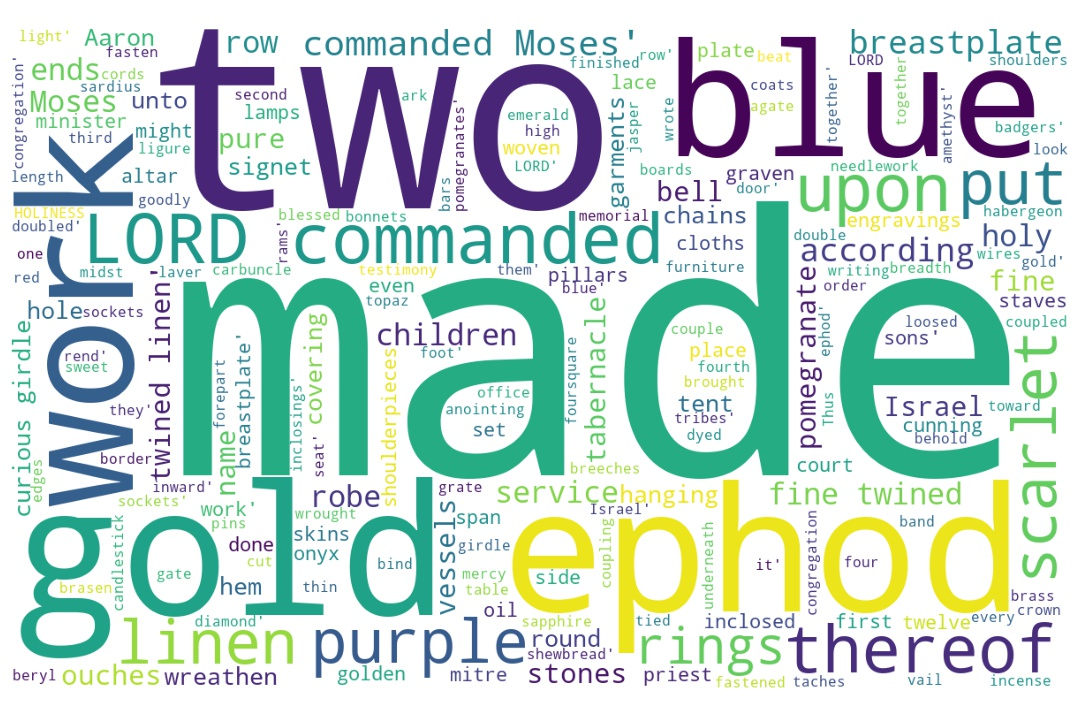
\includegraphics[width=\linewidth]{02OT-Exodus/Exodus39-WordCloud.jpg}
  \caption{Exodus 39 Word Cloud}
  \label{fig:Exodus 39 word Cloud}
\end{figure}


\marginpar{\scriptsize \centering \fcolorbox{bone}{lime}{\textbf{PROJECT ACCEPTANCE}}\\ (Exodus 39:1-43) \begin{compactenum}[I.][8]
    \item A \textbf{Memorial} \index[scripture]{Exodus!Exo 39:07}(Exodus 39:7)  
    \item \textbf{Minute Details} 
    \item The \textbf{Mitre} \index[scripture]{Exodus!Exo 39:28}\index[scripture]{Exodus!Exo 39:31}(Exo 39:28, 31)  
    \item The \textbf{Message} \index[scripture]{Exodus!Exo 39:30}(Exo 39:30)  
    \item \textbf{Mindfulness} \index[scripture]{Exodus!Exo 39:32}(Exo 39:32)  
    \item \textbf{Ministry} \index[scripture]{Exodus!Exo 39:41}(Exo 39:41)  
    \item \textbf{Manifestation} \index[scripture]{Exodus!Exo 39:43}(Exo 39:43)  
\end{compactenum}}




\footnote{\textcolor[cmyk]{0.99998,1,0,0}{\hyperlink{TOC}{Return to end of Table of Contents.}}}\footnote{\href{https://audiobible.com/bible/exodus_39.html}{\textcolor[cmyk]{0.99998,1,0,0}{Exodus 39 Audio}}}\textcolor[cmyk]{0.99998,1,0,0}{And of the blue, and purple, and scarlet, they made cloths of service, to do service in the holy \emph{place}, and made the holy garments for Aaron; as the LORD commanded Moses.}
[2] \textcolor[cmyk]{0.99998,1,0,0}{And he made the ephod \emph{of} \fcolorbox{bone}{bone}{gold}, blue, and purple, and scarlet, and fine twined linen.}
[3] \textcolor[cmyk]{0.99998,1,0,0}{And they did beat the \fcolorbox{bone}{bone}{gold} into thin plates, and cut \emph{it into} wires, to work \emph{it} in the blue, and in the purple, and in the scarlet, and in the fine linen, \emph{with} cunning work.}
[4] \textcolor[cmyk]{0.99998,1,0,0}{They made shoulderpieces for \fcolorbox{bone}{bone}{it}, to couple \emph{it} together: by the two edges was \fcolorbox{bone}{bone}{it} coupled together.}
[5] \textcolor[cmyk]{0.99998,1,0,0}{And the curious girdle of his ephod, that \emph{was} upon \fcolorbox{bone}{bone}{it}, \emph{was} of the same, according to the work thereof; \emph{of} \fcolorbox{bone}{bone}{gold}, blue, and purple, and scarlet, and fine twined linen; as the LORD commanded Moses.}\\
\\
\P \textcolor[cmyk]{0.99998,1,0,0}{And they wrought onyx stones inclosed in ouches of \fcolorbox{bone}{bone}{gold}, graven, as signets are graven, with the names of the children of Israel.}
[7] \textcolor[cmyk]{0.99998,1,0,0}{And he put them on the shoulders of the ephod, \emph{that they should be} stones for a \fcolorbox{bone}{lime}{memorial} to the children of Israel; as the LORD commanded Moses.}\\
\\
\P \textcolor[cmyk]{0.99998,1,0,0}{And he made the breastplate \emph{of} cunning work, like the work of the ephod; \emph{of} \fcolorbox{bone}{bone}{gold}, blue, and purple, and scarlet, and fine twined linen.}
[9] \textcolor[cmyk]{0.99998,1,0,0}{It was foursquare; they made the breastplate double: a span \emph{was} the length thereof, and a span the breadth thereof, \emph{being} doubled.}
[10] \textcolor[cmyk]{0.99998,1,0,0}{And they set in \fcolorbox{bone}{bone}{it} four rows of stones: \emph{the first} row \emph{was} a sardius, a topaz, and a carbuncle: this \emph{was} the first row.}
[11] \textcolor[cmyk]{0.99998,1,0,0}{And the second row, an emerald, a sapphire, and a diamond.}
[12] \textcolor[cmyk]{0.99998,1,0,0}{And the third row, a ligure, an agate, and an amethyst.}
[13] \textcolor[cmyk]{0.99998,1,0,0}{And the fourth row, a beryl, an onyx, and a jasper: \emph{they were} inclosed in ouches of \fcolorbox{bone}{bone}{gold} in their inclosings.}
[14] \textcolor[cmyk]{0.99998,1,0,0}{And the stones \emph{were} according to the names of the children of Israel, twelve, according to their names, \emph{like} the engravings of a signet, every one with his name, according to the twelve tribes.}
[15] \textcolor[cmyk]{0.99998,1,0,0}{And they made upon the breastplate chains at the ends, \emph{of} wreathen work \emph{of} pure \fcolorbox{bone}{bone}{gold}.}
[16] \textcolor[cmyk]{0.99998,1,0,0}{And they made two ouches \emph{of} \fcolorbox{bone}{bone}{gold}, and two \fcolorbox{bone}{bone}{gold} rings; and put the two rings in the two ends of the breastplate.}
[17] \textcolor[cmyk]{0.99998,1,0,0}{And they put the two wreathen chains of \fcolorbox{bone}{bone}{gold} in the two rings on the ends of the breastplate.}
[18] \textcolor[cmyk]{0.99998,1,0,0}{And the two ends of the two wreathen chains they fastened in the two ouches, and put them on the shoulderpieces of the ephod, before \fcolorbox{bone}{bone}{it}.}
[19] \textcolor[cmyk]{0.99998,1,0,0}{And they made two rings of \fcolorbox{bone}{bone}{gold}, and put \emph{them} on the two ends of the breastplate, upon the border of \fcolorbox{bone}{bone}{it}, which \emph{was} on the side of the ephod inward.}
[20] \textcolor[cmyk]{0.99998,1,0,0}{And they made two \emph{other} golden rings, and put them on the two sides of the ephod underneath, toward the forepart of \fcolorbox{bone}{bone}{it}, over against the \emph{other} coupling thereof, above the curious girdle of the ephod.}
[21] \textcolor[cmyk]{0.99998,1,0,0}{And they did bind the breastplate by his rings unto the rings of the ephod with a lace of blue, that \fcolorbox{bone}{bone}{it} might be above the curious girdle of the ephod, and that the breastplate might not be loosed from the ephod; as the LORD commanded Moses.}\\
\\
\P \textcolor[cmyk]{0.99998,1,0,0}{And he made the robe of the ephod \emph{of} woven work, all \emph{of} blue.}
[23] \textcolor[cmyk]{0.99998,1,0,0}{And \emph{there was} an hole in the midst of the robe, as the hole of an habergeon, \emph{with} a band round about the hole, that \fcolorbox{bone}{bone}{it} should not rend.}
[24] \textcolor[cmyk]{0.99998,1,0,0}{And they made upon the hems of the robe pomegranates \emph{of} blue, and purple, and scarlet, \emph{and} twined \emph{linen}.}
[25] \textcolor[cmyk]{0.99998,1,0,0}{And they made bells \emph{of} pure \fcolorbox{bone}{bone}{gold}, and put the bells between the pomegranates upon the hem of the robe, round about between the pomegranates;}
[26] \textcolor[cmyk]{0.99998,1,0,0}{A bell and a pomegranate, a bell and a pomegranate, round about the hem of the robe to minister \emph{in}; as the LORD commanded Moses.}\\
\\
\P \textcolor[cmyk]{0.99998,1,0,0}{And they made coats \emph{of} fine linen \emph{of} woven work for Aaron, and for his sons,}
[28] \textcolor[cmyk]{0.99998,1,0,0}{And a \fcolorbox{bone}{lime}{mre} \emph{of} fine linen, and goodly bonnets \emph{of} fine linen, and linen breeches \emph{of} fine twined linen,}
[29] \textcolor[cmyk]{0.99998,1,0,0}{And a girdle \emph{of} fine twined linen, and blue, and purple, and scarlet, \emph{of} needlework; as the LORD commanded Moses.}\\
\\
\P \textcolor[cmyk]{0.99998,1,0,0}{And they made the plate of the holy crown \emph{of} pure \fcolorbox{bone}{bone}{gold}, and wrote upon \fcolorbox{bone}{bone}{it} \fcolorbox{bone}{lime}{a writing}, \emph{like} \emph{to} the engravings of a signet, HOLINESS TO THE LORD.}
[31] \textcolor[cmyk]{0.99998,1,0,0}{And they tied unto \fcolorbox{bone}{bone}{it} a lace of blue, to fasten \emph{it} on high upon the \fcolorbox{bone}{lime}{mitre}; as the LORD commanded Moses.}\\
\\
\P \textcolor[cmyk]{0.99998,1,0,0}{Thus was all the work of the tabernacle of the tent of the congregation finished: and the children of Israel did \fcolorbox{bone}{lime}{according to} all that the LORD commanded Moses, so did they.}\\
\\
\P \textcolor[cmyk]{0.99998,1,0,0}{And they brought the tabernacle unto Moses, the tent, and all his furniture, his taches, his boards, his bars, and his pillars, and his sockets,}
[34] \textcolor[cmyk]{0.99998,1,0,0}{And the covering of rams' skins dyed red, and the covering of badgers' skins, and the vail of the covering,}
[35] \textcolor[cmyk]{0.99998,1,0,0}{The ark of the testimony, and the staves thereof, and the mercy seat,}
[36] \textcolor[cmyk]{0.99998,1,0,0}{The table, \emph{and} all the vessels thereof, and the shewbread,}
[37] \textcolor[cmyk]{0.99998,1,0,0}{The pure candlestick, \emph{with} the lamps thereof, \emph{even with} the lamps to be set in order, and all the vessels thereof, and the oil for light,}
[38] \textcolor[cmyk]{0.99998,1,0,0}{And the golden altar, and the anointing oil, and the sweet incense, and the hanging for the tabernacle door,}
[39] \textcolor[cmyk]{0.99998,1,0,0}{The brasen altar, and his grate of brass, his staves, and all his vessels, the laver and his foot,}
[40] \textcolor[cmyk]{0.99998,1,0,0}{The hangings of the court, his pillars, and his sockets, and the hanging for the court gate, his cords, and his pins, and all the vessels of the service of the tabernacle, for the tent of the congregation,}
[41] \textcolor[cmyk]{0.99998,1,0,0}{The cloths of service to do service in the holy \emph{place}, and the holy garments for Aaron the priest, and his sons' garments, to \fcolorbox{bone}{lime}{minister} in the priest's office.}
[42] \textcolor[cmyk]{0.99998,1,0,0}{According to all that the LORD commanded Moses, so the children of Israel made all the work.}
[43] \textcolor[cmyk]{0.99998,1,0,0}{And Moses did look upon all the work, and, behold, \fcolorbox{bone}{lime}{they had done \fcolorbox{bone}{bone}{it}} as the LORD had commanded, even so had they done \fcolorbox{bone}{bone}{it}: and Moses blessed them.}
%\index[NWIV]{32!Exodus!Exodus 39:01}\index[AWIP]{And!Exodus!Exodus 39:01}\index[AWIP]{of!Exodus!Exodus 39:01}\index[AWIP]{the!Exodus!Exodus 39:01}\index[AWIP]{blue!Exodus!Exodus 39:01}\index[AWIP]{and!Exodus!Exodus 39:01}\index[AWIP]{purple!Exodus!Exodus 39:01}\index[AWIP]{and!Exodus!Exodus 39:01 (2)}\index[AWIP]{scarlet!Exodus!Exodus 39:01}\index[AWIP]{they!Exodus!Exodus 39:01}\index[AWIP]{made!Exodus!Exodus 39:01}\index[AWIP]{cloths!Exodus!Exodus 39:01}\index[AWIP]{of!Exodus!Exodus 39:01 (2)}\index[AWIP]{service!Exodus!Exodus 39:01}\index[AWIP]{to!Exodus!Exodus 39:01}\index[AWIP]{do!Exodus!Exodus 39:01}\index[AWIP]{service!Exodus!Exodus 39:01 (2)}\index[AWIP]{in!Exodus!Exodus 39:01}\index[AWIP]{the!Exodus!Exodus 39:01 (2)}\index[AWIP]{holy!Exodus!Exodus 39:01}\index[AWIP]{\emph{place}!Exodus!Exodus 39:01}\index[AWIP]{and!Exodus!Exodus 39:01 (3)}\index[AWIP]{made!Exodus!Exodus 39:01 (2)}\index[AWIP]{the!Exodus!Exodus 39:01 (3)}\index[AWIP]{holy!Exodus!Exodus 39:01 (2)}\index[AWIP]{garments!Exodus!Exodus 39:01}\index[AWIP]{for!Exodus!Exodus 39:01}\index[AWIP]{Aaron!Exodus!Exodus 39:01}\index[AWIP]{as!Exodus!Exodus 39:01}\index[AWIP]{the!Exodus!Exodus 39:01 (4)}\index[AWIP]{LORD!Exodus!Exodus 39:01}\index[AWIP]{commanded!Exodus!Exodus 39:01}\index[AWIP]{Moses!Exodus!Exodus 39:01}\index[PNIP]{Aaron!Exodus!Exodus 39:01}\index[PNIP]{LORD!Exodus!Exodus 39:01}\index[PNIP]{Moses!Exodus!Exodus 39:01}

\index[NWIV]{16!Exodus!Exodus 39:02}\index[AWIP]{And!Exodus!Exodus 39:02}\index[AWIP]{he!Exodus!Exodus 39:02}\index[AWIP]{made!Exodus!Exodus 39:02}\index[AWIP]{the!Exodus!Exodus 39:02}\index[AWIP]{ephod!Exodus!Exodus 39:02}\index[AWIP]{\emph{of}!Exodus!Exodus 39:02}\index[AWIP]{gold!Exodus!Exodus 39:02}\index[AWIP]{blue!Exodus!Exodus 39:02}\index[AWIP]{and!Exodus!Exodus 39:02}\index[AWIP]{purple!Exodus!Exodus 39:02}\index[AWIP]{and!Exodus!Exodus 39:02 (2)}\index[AWIP]{scarlet!Exodus!Exodus 39:02}\index[AWIP]{and!Exodus!Exodus 39:02 (3)}\index[AWIP]{fine!Exodus!Exodus 39:02}\index[AWIP]{twined!Exodus!Exodus 39:02}\index[AWIP]{linen!Exodus!Exodus 39:02}

\index[NWIV]{36!Exodus!Exodus 39:03}\index[AWIP]{And!Exodus!Exodus 39:03}\index[AWIP]{they!Exodus!Exodus 39:03}\index[AWIP]{did!Exodus!Exodus 39:03}\index[AWIP]{beat!Exodus!Exodus 39:03}\index[AWIP]{the!Exodus!Exodus 39:03}\index[AWIP]{gold!Exodus!Exodus 39:03}\index[AWIP]{into!Exodus!Exodus 39:03}\index[AWIP]{thin!Exodus!Exodus 39:03}\index[AWIP]{plates!Exodus!Exodus 39:03}\index[AWIP]{and!Exodus!Exodus 39:03}\index[AWIP]{cut!Exodus!Exodus 39:03}\index[AWIP]{\emph{it!Exodus!Exodus 39:03}\index[AWIP]{into}!Exodus!Exodus 39:03}\index[AWIP]{wires!Exodus!Exodus 39:03}\index[AWIP]{to!Exodus!Exodus 39:03}\index[AWIP]{work!Exodus!Exodus 39:03}\index[AWIP]{\emph{it}!Exodus!Exodus 39:03}\index[AWIP]{in!Exodus!Exodus 39:03}\index[AWIP]{the!Exodus!Exodus 39:03 (2)}\index[AWIP]{blue!Exodus!Exodus 39:03}\index[AWIP]{and!Exodus!Exodus 39:03 (2)}\index[AWIP]{in!Exodus!Exodus 39:03 (2)}\index[AWIP]{the!Exodus!Exodus 39:03 (3)}\index[AWIP]{purple!Exodus!Exodus 39:03}\index[AWIP]{and!Exodus!Exodus 39:03 (3)}\index[AWIP]{in!Exodus!Exodus 39:03 (3)}\index[AWIP]{the!Exodus!Exodus 39:03 (4)}\index[AWIP]{scarlet!Exodus!Exodus 39:03}\index[AWIP]{and!Exodus!Exodus 39:03 (4)}\index[AWIP]{in!Exodus!Exodus 39:03 (4)}\index[AWIP]{the!Exodus!Exodus 39:03 (5)}\index[AWIP]{fine!Exodus!Exodus 39:03}\index[AWIP]{linen!Exodus!Exodus 39:03}\index[AWIP]{\emph{with}!Exodus!Exodus 39:03}\index[AWIP]{cunning!Exodus!Exodus 39:03}\index[AWIP]{work!Exodus!Exodus 39:03 (2)}

\index[NWIV]{17!Exodus!Exodus 39:04}\index[AWIP]{They!Exodus!Exodus 39:04}\index[AWIP]{made!Exodus!Exodus 39:04}\index[AWIP]{shoulderpieces!Exodus!Exodus 39:04}\index[AWIP]{for!Exodus!Exodus 39:04}\index[AWIP]{it!Exodus!Exodus 39:04}\index[AWIP]{to!Exodus!Exodus 39:04}\index[AWIP]{couple!Exodus!Exodus 39:04}\index[AWIP]{\emph{it}!Exodus!Exodus 39:04}\index[AWIP]{together!Exodus!Exodus 39:04}\index[AWIP]{by!Exodus!Exodus 39:04}\index[AWIP]{the!Exodus!Exodus 39:04}\index[AWIP]{two!Exodus!Exodus 39:04}\index[AWIP]{edges!Exodus!Exodus 39:04}\index[AWIP]{was!Exodus!Exodus 39:04}\index[AWIP]{it!Exodus!Exodus 39:04 (2)}\index[AWIP]{coupled!Exodus!Exodus 39:04}\index[AWIP]{together!Exodus!Exodus 39:04 (2)}

\index[NWIV]{36!Exodus!Exodus 39:05}\index[AWIP]{And!Exodus!Exodus 39:05}\index[AWIP]{the!Exodus!Exodus 39:05}\index[AWIP]{curious!Exodus!Exodus 39:05}\index[AWIP]{girdle!Exodus!Exodus 39:05}\index[AWIP]{of!Exodus!Exodus 39:05}\index[AWIP]{his!Exodus!Exodus 39:05}\index[AWIP]{ephod!Exodus!Exodus 39:05}\index[AWIP]{that!Exodus!Exodus 39:05}\index[AWIP]{\emph{was}!Exodus!Exodus 39:05}\index[AWIP]{upon!Exodus!Exodus 39:05}\index[AWIP]{it!Exodus!Exodus 39:05}\index[AWIP]{\emph{was}!Exodus!Exodus 39:05 (2)}\index[AWIP]{of!Exodus!Exodus 39:05 (2)}\index[AWIP]{the!Exodus!Exodus 39:05 (2)}\index[AWIP]{same!Exodus!Exodus 39:05}\index[AWIP]{according!Exodus!Exodus 39:05}\index[AWIP]{to!Exodus!Exodus 39:05}\index[AWIP]{the!Exodus!Exodus 39:05 (3)}\index[AWIP]{work!Exodus!Exodus 39:05}\index[AWIP]{thereof!Exodus!Exodus 39:05}\index[AWIP]{\emph{of}!Exodus!Exodus 39:05}\index[AWIP]{gold!Exodus!Exodus 39:05}\index[AWIP]{blue!Exodus!Exodus 39:05}\index[AWIP]{and!Exodus!Exodus 39:05}\index[AWIP]{purple!Exodus!Exodus 39:05}\index[AWIP]{and!Exodus!Exodus 39:05 (2)}\index[AWIP]{scarlet!Exodus!Exodus 39:05}\index[AWIP]{and!Exodus!Exodus 39:05 (3)}\index[AWIP]{fine!Exodus!Exodus 39:05}\index[AWIP]{twined!Exodus!Exodus 39:05}\index[AWIP]{linen!Exodus!Exodus 39:05}\index[AWIP]{as!Exodus!Exodus 39:05}\index[AWIP]{the!Exodus!Exodus 39:05 (4)}\index[AWIP]{LORD!Exodus!Exodus 39:05}\index[AWIP]{commanded!Exodus!Exodus 39:05}\index[AWIP]{Moses!Exodus!Exodus 39:05}\index[PNIP]{LORD!Exodus!Exodus 39:05}\index[PNIP]{Moses!Exodus!Exodus 39:05}

\index[NWIV]{23!Exodus!Exodus 39:06}\index[AWIP]{And!Exodus!Exodus 39:06}\index[AWIP]{they!Exodus!Exodus 39:06}\index[AWIP]{wrought!Exodus!Exodus 39:06}\index[AWIP]{onyx!Exodus!Exodus 39:06}\index[AWIP]{stones!Exodus!Exodus 39:06}\index[AWIP]{inclosed!Exodus!Exodus 39:06}\index[AWIP]{in!Exodus!Exodus 39:06}\index[AWIP]{ouches!Exodus!Exodus 39:06}\index[AWIP]{of!Exodus!Exodus 39:06}\index[AWIP]{gold!Exodus!Exodus 39:06}\index[AWIP]{graven!Exodus!Exodus 39:06}\index[AWIP]{as!Exodus!Exodus 39:06}\index[AWIP]{signets!Exodus!Exodus 39:06}\index[AWIP]{are!Exodus!Exodus 39:06}\index[AWIP]{graven!Exodus!Exodus 39:06 (2)}\index[AWIP]{with!Exodus!Exodus 39:06}\index[AWIP]{the!Exodus!Exodus 39:06}\index[AWIP]{names!Exodus!Exodus 39:06}\index[AWIP]{of!Exodus!Exodus 39:06 (2)}\index[AWIP]{the!Exodus!Exodus 39:06 (2)}\index[AWIP]{children!Exodus!Exodus 39:06}\index[AWIP]{of!Exodus!Exodus 39:06 (3)}\index[AWIP]{Israel!Exodus!Exodus 39:06}\index[PNIP]{Israel!Exodus!Exodus 39:06}

\index[NWIV]{28!Exodus!Exodus 39:07}\index[AWIP]{And!Exodus!Exodus 39:07}\index[AWIP]{he!Exodus!Exodus 39:07}\index[AWIP]{put!Exodus!Exodus 39:07}\index[AWIP]{them!Exodus!Exodus 39:07}\index[AWIP]{on!Exodus!Exodus 39:07}\index[AWIP]{the!Exodus!Exodus 39:07}\index[AWIP]{shoulders!Exodus!Exodus 39:07}\index[AWIP]{of!Exodus!Exodus 39:07}\index[AWIP]{the!Exodus!Exodus 39:07 (2)}\index[AWIP]{ephod!Exodus!Exodus 39:07}\index[AWIP]{\emph{that!Exodus!Exodus 39:07}\index[AWIP]{they!Exodus!Exodus 39:07}\index[AWIP]{should!Exodus!Exodus 39:07}\index[AWIP]{be}!Exodus!Exodus 39:07}\index[AWIP]{stones!Exodus!Exodus 39:07}\index[AWIP]{for!Exodus!Exodus 39:07}\index[AWIP]{a!Exodus!Exodus 39:07}\index[AWIP]{memorial!Exodus!Exodus 39:07}\index[AWIP]{to!Exodus!Exodus 39:07}\index[AWIP]{the!Exodus!Exodus 39:07 (3)}\index[AWIP]{children!Exodus!Exodus 39:07}\index[AWIP]{of!Exodus!Exodus 39:07 (2)}\index[AWIP]{Israel!Exodus!Exodus 39:07}\index[AWIP]{as!Exodus!Exodus 39:07}\index[AWIP]{the!Exodus!Exodus 39:07 (4)}\index[AWIP]{LORD!Exodus!Exodus 39:07}\index[AWIP]{commanded!Exodus!Exodus 39:07}\index[AWIP]{Moses!Exodus!Exodus 39:07}\index[PNIP]{Israel!Exodus!Exodus 39:07}\index[PNIP]{LORD!Exodus!Exodus 39:07}\index[PNIP]{Moses!Exodus!Exodus 39:07}

\index[NWIV]{25!Exodus!Exodus 39:08}\index[AWIP]{And!Exodus!Exodus 39:08}\index[AWIP]{he!Exodus!Exodus 39:08}\index[AWIP]{made!Exodus!Exodus 39:08}\index[AWIP]{the!Exodus!Exodus 39:08}\index[AWIP]{breastplate!Exodus!Exodus 39:08}\index[AWIP]{\emph{of}!Exodus!Exodus 39:08}\index[AWIP]{cunning!Exodus!Exodus 39:08}\index[AWIP]{work!Exodus!Exodus 39:08}\index[AWIP]{like!Exodus!Exodus 39:08}\index[AWIP]{the!Exodus!Exodus 39:08 (2)}\index[AWIP]{work!Exodus!Exodus 39:08 (2)}\index[AWIP]{of!Exodus!Exodus 39:08}\index[AWIP]{the!Exodus!Exodus 39:08 (3)}\index[AWIP]{ephod!Exodus!Exodus 39:08}\index[AWIP]{\emph{of}!Exodus!Exodus 39:08 (2)}\index[AWIP]{gold!Exodus!Exodus 39:08}\index[AWIP]{blue!Exodus!Exodus 39:08}\index[AWIP]{and!Exodus!Exodus 39:08}\index[AWIP]{purple!Exodus!Exodus 39:08}\index[AWIP]{and!Exodus!Exodus 39:08 (2)}\index[AWIP]{scarlet!Exodus!Exodus 39:08}\index[AWIP]{and!Exodus!Exodus 39:08 (3)}\index[AWIP]{fine!Exodus!Exodus 39:08}\index[AWIP]{twined!Exodus!Exodus 39:08}\index[AWIP]{linen!Exodus!Exodus 39:08}

\index[NWIV]{22!Exodus!Exodus 39:09}\index[AWIP]{It!Exodus!Exodus 39:09}\index[AWIP]{was!Exodus!Exodus 39:09}\index[AWIP]{foursquare!Exodus!Exodus 39:09}\index[AWIP]{they!Exodus!Exodus 39:09}\index[AWIP]{made!Exodus!Exodus 39:09}\index[AWIP]{the!Exodus!Exodus 39:09}\index[AWIP]{breastplate!Exodus!Exodus 39:09}\index[AWIP]{double!Exodus!Exodus 39:09}\index[AWIP]{a!Exodus!Exodus 39:09}\index[AWIP]{span!Exodus!Exodus 39:09}\index[AWIP]{\emph{was}!Exodus!Exodus 39:09}\index[AWIP]{the!Exodus!Exodus 39:09 (2)}\index[AWIP]{length!Exodus!Exodus 39:09}\index[AWIP]{thereof!Exodus!Exodus 39:09}\index[AWIP]{and!Exodus!Exodus 39:09}\index[AWIP]{a!Exodus!Exodus 39:09 (2)}\index[AWIP]{span!Exodus!Exodus 39:09 (2)}\index[AWIP]{the!Exodus!Exodus 39:09 (3)}\index[AWIP]{breadth!Exodus!Exodus 39:09}\index[AWIP]{thereof!Exodus!Exodus 39:09 (2)}\index[AWIP]{\emph{being}!Exodus!Exodus 39:09}\index[AWIP]{doubled!Exodus!Exodus 39:09}

\index[NWIV]{25!Exodus!Exodus 39:10}\index[AWIP]{And!Exodus!Exodus 39:10}\index[AWIP]{they!Exodus!Exodus 39:10}\index[AWIP]{set!Exodus!Exodus 39:10}\index[AWIP]{in!Exodus!Exodus 39:10}\index[AWIP]{it!Exodus!Exodus 39:10}\index[AWIP]{four!Exodus!Exodus 39:10}\index[AWIP]{rows!Exodus!Exodus 39:10}\index[AWIP]{of!Exodus!Exodus 39:10}\index[AWIP]{stones!Exodus!Exodus 39:10}\index[AWIP]{\emph{the!Exodus!Exodus 39:10}\index[AWIP]{first}!Exodus!Exodus 39:10}\index[AWIP]{row!Exodus!Exodus 39:10}\index[AWIP]{\emph{was}!Exodus!Exodus 39:10}\index[AWIP]{a!Exodus!Exodus 39:10}\index[AWIP]{sardius!Exodus!Exodus 39:10}\index[AWIP]{a!Exodus!Exodus 39:10 (2)}\index[AWIP]{topaz!Exodus!Exodus 39:10}\index[AWIP]{and!Exodus!Exodus 39:10}\index[AWIP]{a!Exodus!Exodus 39:10 (3)}\index[AWIP]{carbuncle!Exodus!Exodus 39:10}\index[AWIP]{this!Exodus!Exodus 39:10}\index[AWIP]{\emph{was}!Exodus!Exodus 39:10 (2)}\index[AWIP]{the!Exodus!Exodus 39:10}\index[AWIP]{first!Exodus!Exodus 39:10}\index[AWIP]{row!Exodus!Exodus 39:10 (2)}

\index[NWIV]{11!Exodus!Exodus 39:11}\index[AWIP]{And!Exodus!Exodus 39:11}\index[AWIP]{the!Exodus!Exodus 39:11}\index[AWIP]{second!Exodus!Exodus 39:11}\index[AWIP]{row!Exodus!Exodus 39:11}\index[AWIP]{an!Exodus!Exodus 39:11}\index[AWIP]{emerald!Exodus!Exodus 39:11}\index[AWIP]{a!Exodus!Exodus 39:11}\index[AWIP]{sapphire!Exodus!Exodus 39:11}\index[AWIP]{and!Exodus!Exodus 39:11}\index[AWIP]{a!Exodus!Exodus 39:11 (2)}\index[AWIP]{diamond!Exodus!Exodus 39:11}

\index[NWIV]{11!Exodus!Exodus 39:12}\index[AWIP]{And!Exodus!Exodus 39:12}\index[AWIP]{the!Exodus!Exodus 39:12}\index[AWIP]{third!Exodus!Exodus 39:12}\index[AWIP]{row!Exodus!Exodus 39:12}\index[AWIP]{a!Exodus!Exodus 39:12}\index[AWIP]{ligure!Exodus!Exodus 39:12}\index[AWIP]{an!Exodus!Exodus 39:12}\index[AWIP]{agate!Exodus!Exodus 39:12}\index[AWIP]{and!Exodus!Exodus 39:12}\index[AWIP]{an!Exodus!Exodus 39:12 (2)}\index[AWIP]{amethyst!Exodus!Exodus 39:12}

\index[NWIV]{21!Exodus!Exodus 39:13}\index[AWIP]{And!Exodus!Exodus 39:13}\index[AWIP]{the!Exodus!Exodus 39:13}\index[AWIP]{fourth!Exodus!Exodus 39:13}\index[AWIP]{row!Exodus!Exodus 39:13}\index[AWIP]{a!Exodus!Exodus 39:13}\index[AWIP]{beryl!Exodus!Exodus 39:13}\index[AWIP]{an!Exodus!Exodus 39:13}\index[AWIP]{onyx!Exodus!Exodus 39:13}\index[AWIP]{and!Exodus!Exodus 39:13}\index[AWIP]{a!Exodus!Exodus 39:13 (2)}\index[AWIP]{jasper!Exodus!Exodus 39:13}\index[AWIP]{\emph{they!Exodus!Exodus 39:13}\index[AWIP]{were}!Exodus!Exodus 39:13}\index[AWIP]{inclosed!Exodus!Exodus 39:13}\index[AWIP]{in!Exodus!Exodus 39:13}\index[AWIP]{ouches!Exodus!Exodus 39:13}\index[AWIP]{of!Exodus!Exodus 39:13}\index[AWIP]{gold!Exodus!Exodus 39:13}\index[AWIP]{in!Exodus!Exodus 39:13 (2)}\index[AWIP]{their!Exodus!Exodus 39:13}\index[AWIP]{inclosings!Exodus!Exodus 39:13}

\index[NWIV]{34!Exodus!Exodus 39:14}\index[AWIP]{And!Exodus!Exodus 39:14}\index[AWIP]{the!Exodus!Exodus 39:14}\index[AWIP]{stones!Exodus!Exodus 39:14}\index[AWIP]{\emph{were}!Exodus!Exodus 39:14}\index[AWIP]{according!Exodus!Exodus 39:14}\index[AWIP]{to!Exodus!Exodus 39:14}\index[AWIP]{the!Exodus!Exodus 39:14 (2)}\index[AWIP]{names!Exodus!Exodus 39:14}\index[AWIP]{of!Exodus!Exodus 39:14}\index[AWIP]{the!Exodus!Exodus 39:14 (3)}\index[AWIP]{children!Exodus!Exodus 39:14}\index[AWIP]{of!Exodus!Exodus 39:14 (2)}\index[AWIP]{Israel!Exodus!Exodus 39:14}\index[AWIP]{twelve!Exodus!Exodus 39:14}\index[AWIP]{according!Exodus!Exodus 39:14 (2)}\index[AWIP]{to!Exodus!Exodus 39:14 (2)}\index[AWIP]{their!Exodus!Exodus 39:14}\index[AWIP]{names!Exodus!Exodus 39:14 (2)}\index[AWIP]{\emph{like}!Exodus!Exodus 39:14}\index[AWIP]{the!Exodus!Exodus 39:14 (4)}\index[AWIP]{engravings!Exodus!Exodus 39:14}\index[AWIP]{of!Exodus!Exodus 39:14 (3)}\index[AWIP]{a!Exodus!Exodus 39:14}\index[AWIP]{signet!Exodus!Exodus 39:14}\index[AWIP]{every!Exodus!Exodus 39:14}\index[AWIP]{one!Exodus!Exodus 39:14}\index[AWIP]{with!Exodus!Exodus 39:14}\index[AWIP]{his!Exodus!Exodus 39:14}\index[AWIP]{name!Exodus!Exodus 39:14}\index[AWIP]{according!Exodus!Exodus 39:14 (3)}\index[AWIP]{to!Exodus!Exodus 39:14 (3)}\index[AWIP]{the!Exodus!Exodus 39:14 (5)}\index[AWIP]{twelve!Exodus!Exodus 39:14 (2)}\index[AWIP]{tribes!Exodus!Exodus 39:14}\index[PNIP]{Israel!Exodus!Exodus 39:14}

\index[NWIV]{16!Exodus!Exodus 39:15}\index[AWIP]{And!Exodus!Exodus 39:15}\index[AWIP]{they!Exodus!Exodus 39:15}\index[AWIP]{made!Exodus!Exodus 39:15}\index[AWIP]{upon!Exodus!Exodus 39:15}\index[AWIP]{the!Exodus!Exodus 39:15}\index[AWIP]{breastplate!Exodus!Exodus 39:15}\index[AWIP]{chains!Exodus!Exodus 39:15}\index[AWIP]{at!Exodus!Exodus 39:15}\index[AWIP]{the!Exodus!Exodus 39:15 (2)}\index[AWIP]{ends!Exodus!Exodus 39:15}\index[AWIP]{\emph{of}!Exodus!Exodus 39:15}\index[AWIP]{wreathen!Exodus!Exodus 39:15}\index[AWIP]{work!Exodus!Exodus 39:15}\index[AWIP]{\emph{of}!Exodus!Exodus 39:15 (2)}\index[AWIP]{pure!Exodus!Exodus 39:15}\index[AWIP]{gold!Exodus!Exodus 39:15}

\index[NWIV]{23!Exodus!Exodus 39:16}\index[AWIP]{And!Exodus!Exodus 39:16}\index[AWIP]{they!Exodus!Exodus 39:16}\index[AWIP]{made!Exodus!Exodus 39:16}\index[AWIP]{two!Exodus!Exodus 39:16}\index[AWIP]{ouches!Exodus!Exodus 39:16}\index[AWIP]{\emph{of}!Exodus!Exodus 39:16}\index[AWIP]{gold!Exodus!Exodus 39:16}\index[AWIP]{and!Exodus!Exodus 39:16}\index[AWIP]{two!Exodus!Exodus 39:16 (2)}\index[AWIP]{gold!Exodus!Exodus 39:16 (2)}\index[AWIP]{rings!Exodus!Exodus 39:16}\index[AWIP]{and!Exodus!Exodus 39:16 (2)}\index[AWIP]{put!Exodus!Exodus 39:16}\index[AWIP]{the!Exodus!Exodus 39:16}\index[AWIP]{two!Exodus!Exodus 39:16 (3)}\index[AWIP]{rings!Exodus!Exodus 39:16 (2)}\index[AWIP]{in!Exodus!Exodus 39:16}\index[AWIP]{the!Exodus!Exodus 39:16 (2)}\index[AWIP]{two!Exodus!Exodus 39:16 (4)}\index[AWIP]{ends!Exodus!Exodus 39:16}\index[AWIP]{of!Exodus!Exodus 39:16}\index[AWIP]{the!Exodus!Exodus 39:16 (3)}\index[AWIP]{breastplate!Exodus!Exodus 39:16}

\index[NWIV]{19!Exodus!Exodus 39:17}\index[AWIP]{And!Exodus!Exodus 39:17}\index[AWIP]{they!Exodus!Exodus 39:17}\index[AWIP]{put!Exodus!Exodus 39:17}\index[AWIP]{the!Exodus!Exodus 39:17}\index[AWIP]{two!Exodus!Exodus 39:17}\index[AWIP]{wreathen!Exodus!Exodus 39:17}\index[AWIP]{chains!Exodus!Exodus 39:17}\index[AWIP]{of!Exodus!Exodus 39:17}\index[AWIP]{gold!Exodus!Exodus 39:17}\index[AWIP]{in!Exodus!Exodus 39:17}\index[AWIP]{the!Exodus!Exodus 39:17 (2)}\index[AWIP]{two!Exodus!Exodus 39:17 (2)}\index[AWIP]{rings!Exodus!Exodus 39:17}\index[AWIP]{on!Exodus!Exodus 39:17}\index[AWIP]{the!Exodus!Exodus 39:17 (3)}\index[AWIP]{ends!Exodus!Exodus 39:17}\index[AWIP]{of!Exodus!Exodus 39:17 (2)}\index[AWIP]{the!Exodus!Exodus 39:17 (4)}\index[AWIP]{breastplate!Exodus!Exodus 39:17}

\index[NWIV]{26!Exodus!Exodus 39:18}\index[AWIP]{And!Exodus!Exodus 39:18}\index[AWIP]{the!Exodus!Exodus 39:18}\index[AWIP]{two!Exodus!Exodus 39:18}\index[AWIP]{ends!Exodus!Exodus 39:18}\index[AWIP]{of!Exodus!Exodus 39:18}\index[AWIP]{the!Exodus!Exodus 39:18 (2)}\index[AWIP]{two!Exodus!Exodus 39:18 (2)}\index[AWIP]{wreathen!Exodus!Exodus 39:18}\index[AWIP]{chains!Exodus!Exodus 39:18}\index[AWIP]{they!Exodus!Exodus 39:18}\index[AWIP]{fastened!Exodus!Exodus 39:18}\index[AWIP]{in!Exodus!Exodus 39:18}\index[AWIP]{the!Exodus!Exodus 39:18 (3)}\index[AWIP]{two!Exodus!Exodus 39:18 (3)}\index[AWIP]{ouches!Exodus!Exodus 39:18}\index[AWIP]{and!Exodus!Exodus 39:18}\index[AWIP]{put!Exodus!Exodus 39:18}\index[AWIP]{them!Exodus!Exodus 39:18}\index[AWIP]{on!Exodus!Exodus 39:18}\index[AWIP]{the!Exodus!Exodus 39:18 (4)}\index[AWIP]{shoulderpieces!Exodus!Exodus 39:18}\index[AWIP]{of!Exodus!Exodus 39:18 (2)}\index[AWIP]{the!Exodus!Exodus 39:18 (5)}\index[AWIP]{ephod!Exodus!Exodus 39:18}\index[AWIP]{before!Exodus!Exodus 39:18}\index[AWIP]{it!Exodus!Exodus 39:18}

\index[NWIV]{31!Exodus!Exodus 39:19}\index[AWIP]{And!Exodus!Exodus 39:19}\index[AWIP]{they!Exodus!Exodus 39:19}\index[AWIP]{made!Exodus!Exodus 39:19}\index[AWIP]{two!Exodus!Exodus 39:19}\index[AWIP]{rings!Exodus!Exodus 39:19}\index[AWIP]{of!Exodus!Exodus 39:19}\index[AWIP]{gold!Exodus!Exodus 39:19}\index[AWIP]{and!Exodus!Exodus 39:19}\index[AWIP]{put!Exodus!Exodus 39:19}\index[AWIP]{\emph{them}!Exodus!Exodus 39:19}\index[AWIP]{on!Exodus!Exodus 39:19}\index[AWIP]{the!Exodus!Exodus 39:19}\index[AWIP]{two!Exodus!Exodus 39:19 (2)}\index[AWIP]{ends!Exodus!Exodus 39:19}\index[AWIP]{of!Exodus!Exodus 39:19 (2)}\index[AWIP]{the!Exodus!Exodus 39:19 (2)}\index[AWIP]{breastplate!Exodus!Exodus 39:19}\index[AWIP]{upon!Exodus!Exodus 39:19}\index[AWIP]{the!Exodus!Exodus 39:19 (3)}\index[AWIP]{border!Exodus!Exodus 39:19}\index[AWIP]{of!Exodus!Exodus 39:19 (3)}\index[AWIP]{it!Exodus!Exodus 39:19}\index[AWIP]{which!Exodus!Exodus 39:19}\index[AWIP]{\emph{was}!Exodus!Exodus 39:19}\index[AWIP]{on!Exodus!Exodus 39:19 (2)}\index[AWIP]{the!Exodus!Exodus 39:19 (4)}\index[AWIP]{side!Exodus!Exodus 39:19}\index[AWIP]{of!Exodus!Exodus 39:19 (4)}\index[AWIP]{the!Exodus!Exodus 39:19 (5)}\index[AWIP]{ephod!Exodus!Exodus 39:19}\index[AWIP]{inward!Exodus!Exodus 39:19}

\index[NWIV]{36!Exodus!Exodus 39:20}\index[AWIP]{And!Exodus!Exodus 39:20}\index[AWIP]{they!Exodus!Exodus 39:20}\index[AWIP]{made!Exodus!Exodus 39:20}\index[AWIP]{two!Exodus!Exodus 39:20}\index[AWIP]{\emph{other}!Exodus!Exodus 39:20}\index[AWIP]{golden!Exodus!Exodus 39:20}\index[AWIP]{rings!Exodus!Exodus 39:20}\index[AWIP]{and!Exodus!Exodus 39:20}\index[AWIP]{put!Exodus!Exodus 39:20}\index[AWIP]{them!Exodus!Exodus 39:20}\index[AWIP]{on!Exodus!Exodus 39:20}\index[AWIP]{the!Exodus!Exodus 39:20}\index[AWIP]{two!Exodus!Exodus 39:20 (2)}\index[AWIP]{sides!Exodus!Exodus 39:20}\index[AWIP]{of!Exodus!Exodus 39:20}\index[AWIP]{the!Exodus!Exodus 39:20 (2)}\index[AWIP]{ephod!Exodus!Exodus 39:20}\index[AWIP]{underneath!Exodus!Exodus 39:20}\index[AWIP]{toward!Exodus!Exodus 39:20}\index[AWIP]{the!Exodus!Exodus 39:20 (3)}\index[AWIP]{forepart!Exodus!Exodus 39:20}\index[AWIP]{of!Exodus!Exodus 39:20 (2)}\index[AWIP]{it!Exodus!Exodus 39:20}\index[AWIP]{over!Exodus!Exodus 39:20}\index[AWIP]{against!Exodus!Exodus 39:20}\index[AWIP]{the!Exodus!Exodus 39:20 (4)}\index[AWIP]{\emph{other}!Exodus!Exodus 39:20 (2)}\index[AWIP]{coupling!Exodus!Exodus 39:20}\index[AWIP]{thereof!Exodus!Exodus 39:20}\index[AWIP]{above!Exodus!Exodus 39:20}\index[AWIP]{the!Exodus!Exodus 39:20 (5)}\index[AWIP]{curious!Exodus!Exodus 39:20}\index[AWIP]{girdle!Exodus!Exodus 39:20}\index[AWIP]{of!Exodus!Exodus 39:20 (3)}\index[AWIP]{the!Exodus!Exodus 39:20 (6)}\index[AWIP]{ephod!Exodus!Exodus 39:20 (2)}

\index[NWIV]{47!Exodus!Exodus 39:21}\index[AWIP]{And!Exodus!Exodus 39:21}\index[AWIP]{they!Exodus!Exodus 39:21}\index[AWIP]{did!Exodus!Exodus 39:21}\index[AWIP]{bind!Exodus!Exodus 39:21}\index[AWIP]{the!Exodus!Exodus 39:21}\index[AWIP]{breastplate!Exodus!Exodus 39:21}\index[AWIP]{by!Exodus!Exodus 39:21}\index[AWIP]{his!Exodus!Exodus 39:21}\index[AWIP]{rings!Exodus!Exodus 39:21}\index[AWIP]{unto!Exodus!Exodus 39:21}\index[AWIP]{the!Exodus!Exodus 39:21 (2)}\index[AWIP]{rings!Exodus!Exodus 39:21 (2)}\index[AWIP]{of!Exodus!Exodus 39:21}\index[AWIP]{the!Exodus!Exodus 39:21 (3)}\index[AWIP]{ephod!Exodus!Exodus 39:21}\index[AWIP]{with!Exodus!Exodus 39:21}\index[AWIP]{a!Exodus!Exodus 39:21}\index[AWIP]{lace!Exodus!Exodus 39:21}\index[AWIP]{of!Exodus!Exodus 39:21 (2)}\index[AWIP]{blue!Exodus!Exodus 39:21}\index[AWIP]{that!Exodus!Exodus 39:21}\index[AWIP]{it!Exodus!Exodus 39:21}\index[AWIP]{might!Exodus!Exodus 39:21}\index[AWIP]{be!Exodus!Exodus 39:21}\index[AWIP]{above!Exodus!Exodus 39:21}\index[AWIP]{the!Exodus!Exodus 39:21 (4)}\index[AWIP]{curious!Exodus!Exodus 39:21}\index[AWIP]{girdle!Exodus!Exodus 39:21}\index[AWIP]{of!Exodus!Exodus 39:21 (3)}\index[AWIP]{the!Exodus!Exodus 39:21 (5)}\index[AWIP]{ephod!Exodus!Exodus 39:21 (2)}\index[AWIP]{and!Exodus!Exodus 39:21}\index[AWIP]{that!Exodus!Exodus 39:21 (2)}\index[AWIP]{the!Exodus!Exodus 39:21 (6)}\index[AWIP]{breastplate!Exodus!Exodus 39:21 (2)}\index[AWIP]{might!Exodus!Exodus 39:21 (2)}\index[AWIP]{not!Exodus!Exodus 39:21}\index[AWIP]{be!Exodus!Exodus 39:21 (2)}\index[AWIP]{loosed!Exodus!Exodus 39:21}\index[AWIP]{from!Exodus!Exodus 39:21}\index[AWIP]{the!Exodus!Exodus 39:21 (7)}\index[AWIP]{ephod!Exodus!Exodus 39:21 (3)}\index[AWIP]{as!Exodus!Exodus 39:21}\index[AWIP]{the!Exodus!Exodus 39:21 (8)}\index[AWIP]{LORD!Exodus!Exodus 39:21}\index[AWIP]{commanded!Exodus!Exodus 39:21}\index[AWIP]{Moses!Exodus!Exodus 39:21}\index[PNIP]{LORD!Exodus!Exodus 39:21}\index[PNIP]{Moses!Exodus!Exodus 39:21}

\index[NWIV]{14!Exodus!Exodus 39:22}\index[AWIP]{And!Exodus!Exodus 39:22}\index[AWIP]{he!Exodus!Exodus 39:22}\index[AWIP]{made!Exodus!Exodus 39:22}\index[AWIP]{the!Exodus!Exodus 39:22}\index[AWIP]{robe!Exodus!Exodus 39:22}\index[AWIP]{of!Exodus!Exodus 39:22}\index[AWIP]{the!Exodus!Exodus 39:22 (2)}\index[AWIP]{ephod!Exodus!Exodus 39:22}\index[AWIP]{\emph{of}!Exodus!Exodus 39:22}\index[AWIP]{woven!Exodus!Exodus 39:22}\index[AWIP]{work!Exodus!Exodus 39:22}\index[AWIP]{all!Exodus!Exodus 39:22}\index[AWIP]{\emph{of}!Exodus!Exodus 39:22 (2)}\index[AWIP]{blue!Exodus!Exodus 39:22}

\index[NWIV]{29!Exodus!Exodus 39:23}\index[AWIP]{And!Exodus!Exodus 39:23}\index[AWIP]{\emph{there!Exodus!Exodus 39:23}\index[AWIP]{was}!Exodus!Exodus 39:23}\index[AWIP]{an!Exodus!Exodus 39:23}\index[AWIP]{hole!Exodus!Exodus 39:23}\index[AWIP]{in!Exodus!Exodus 39:23}\index[AWIP]{the!Exodus!Exodus 39:23}\index[AWIP]{midst!Exodus!Exodus 39:23}\index[AWIP]{of!Exodus!Exodus 39:23}\index[AWIP]{the!Exodus!Exodus 39:23 (2)}\index[AWIP]{robe!Exodus!Exodus 39:23}\index[AWIP]{as!Exodus!Exodus 39:23}\index[AWIP]{the!Exodus!Exodus 39:23 (3)}\index[AWIP]{hole!Exodus!Exodus 39:23 (2)}\index[AWIP]{of!Exodus!Exodus 39:23 (2)}\index[AWIP]{an!Exodus!Exodus 39:23 (2)}\index[AWIP]{habergeon!Exodus!Exodus 39:23}\index[AWIP]{\emph{with}!Exodus!Exodus 39:23}\index[AWIP]{a!Exodus!Exodus 39:23}\index[AWIP]{band!Exodus!Exodus 39:23}\index[AWIP]{round!Exodus!Exodus 39:23}\index[AWIP]{about!Exodus!Exodus 39:23}\index[AWIP]{the!Exodus!Exodus 39:23 (4)}\index[AWIP]{hole!Exodus!Exodus 39:23 (3)}\index[AWIP]{that!Exodus!Exodus 39:23}\index[AWIP]{it!Exodus!Exodus 39:23}\index[AWIP]{should!Exodus!Exodus 39:23}\index[AWIP]{not!Exodus!Exodus 39:23}\index[AWIP]{rend!Exodus!Exodus 39:23}

\index[NWIV]{19!Exodus!Exodus 39:24}\index[AWIP]{And!Exodus!Exodus 39:24}\index[AWIP]{they!Exodus!Exodus 39:24}\index[AWIP]{made!Exodus!Exodus 39:24}\index[AWIP]{upon!Exodus!Exodus 39:24}\index[AWIP]{the!Exodus!Exodus 39:24}\index[AWIP]{hems!Exodus!Exodus 39:24}\index[AWIP]{of!Exodus!Exodus 39:24}\index[AWIP]{the!Exodus!Exodus 39:24 (2)}\index[AWIP]{robe!Exodus!Exodus 39:24}\index[AWIP]{pomegranates!Exodus!Exodus 39:24}\index[AWIP]{\emph{of}!Exodus!Exodus 39:24}\index[AWIP]{blue!Exodus!Exodus 39:24}\index[AWIP]{and!Exodus!Exodus 39:24}\index[AWIP]{purple!Exodus!Exodus 39:24}\index[AWIP]{and!Exodus!Exodus 39:24 (2)}\index[AWIP]{scarlet!Exodus!Exodus 39:24}\index[AWIP]{\emph{and}!Exodus!Exodus 39:24}\index[AWIP]{twined!Exodus!Exodus 39:24}\index[AWIP]{\emph{linen}!Exodus!Exodus 39:24}

\index[NWIV]{25!Exodus!Exodus 39:25}\index[AWIP]{And!Exodus!Exodus 39:25}\index[AWIP]{they!Exodus!Exodus 39:25}\index[AWIP]{made!Exodus!Exodus 39:25}\index[AWIP]{bells!Exodus!Exodus 39:25}\index[AWIP]{\emph{of}!Exodus!Exodus 39:25}\index[AWIP]{pure!Exodus!Exodus 39:25}\index[AWIP]{gold!Exodus!Exodus 39:25}\index[AWIP]{and!Exodus!Exodus 39:25}\index[AWIP]{put!Exodus!Exodus 39:25}\index[AWIP]{the!Exodus!Exodus 39:25}\index[AWIP]{bells!Exodus!Exodus 39:25 (2)}\index[AWIP]{between!Exodus!Exodus 39:25}\index[AWIP]{the!Exodus!Exodus 39:25 (2)}\index[AWIP]{pomegranates!Exodus!Exodus 39:25}\index[AWIP]{upon!Exodus!Exodus 39:25}\index[AWIP]{the!Exodus!Exodus 39:25 (3)}\index[AWIP]{hem!Exodus!Exodus 39:25}\index[AWIP]{of!Exodus!Exodus 39:25}\index[AWIP]{the!Exodus!Exodus 39:25 (4)}\index[AWIP]{robe!Exodus!Exodus 39:25}\index[AWIP]{round!Exodus!Exodus 39:25}\index[AWIP]{about!Exodus!Exodus 39:25}\index[AWIP]{between!Exodus!Exodus 39:25 (2)}\index[AWIP]{the!Exodus!Exodus 39:25 (5)}\index[AWIP]{pomegranates!Exodus!Exodus 39:25 (2)}

\index[NWIV]{25!Exodus!Exodus 39:26}\index[AWIP]{A!Exodus!Exodus 39:26}\index[AWIP]{bell!Exodus!Exodus 39:26}\index[AWIP]{and!Exodus!Exodus 39:26}\index[AWIP]{a!Exodus!Exodus 39:26}\index[AWIP]{pomegranate!Exodus!Exodus 39:26}\index[AWIP]{a!Exodus!Exodus 39:26 (2)}\index[AWIP]{bell!Exodus!Exodus 39:26 (2)}\index[AWIP]{and!Exodus!Exodus 39:26 (2)}\index[AWIP]{a!Exodus!Exodus 39:26 (3)}\index[AWIP]{pomegranate!Exodus!Exodus 39:26 (2)}\index[AWIP]{round!Exodus!Exodus 39:26}\index[AWIP]{about!Exodus!Exodus 39:26}\index[AWIP]{the!Exodus!Exodus 39:26}\index[AWIP]{hem!Exodus!Exodus 39:26}\index[AWIP]{of!Exodus!Exodus 39:26}\index[AWIP]{the!Exodus!Exodus 39:26 (2)}\index[AWIP]{robe!Exodus!Exodus 39:26}\index[AWIP]{to!Exodus!Exodus 39:26}\index[AWIP]{minister!Exodus!Exodus 39:26}\index[AWIP]{\emph{in}!Exodus!Exodus 39:26}\index[AWIP]{as!Exodus!Exodus 39:26}\index[AWIP]{the!Exodus!Exodus 39:26 (3)}\index[AWIP]{LORD!Exodus!Exodus 39:26}\index[AWIP]{commanded!Exodus!Exodus 39:26}\index[AWIP]{Moses!Exodus!Exodus 39:26}\index[PNIP]{LORD!Exodus!Exodus 39:26}\index[PNIP]{Moses!Exodus!Exodus 39:26}

\index[NWIV]{16!Exodus!Exodus 39:27}\index[AWIP]{And!Exodus!Exodus 39:27}\index[AWIP]{they!Exodus!Exodus 39:27}\index[AWIP]{made!Exodus!Exodus 39:27}\index[AWIP]{coats!Exodus!Exodus 39:27}\index[AWIP]{\emph{of}!Exodus!Exodus 39:27}\index[AWIP]{fine!Exodus!Exodus 39:27}\index[AWIP]{linen!Exodus!Exodus 39:27}\index[AWIP]{\emph{of}!Exodus!Exodus 39:27 (2)}\index[AWIP]{woven!Exodus!Exodus 39:27}\index[AWIP]{work!Exodus!Exodus 39:27}\index[AWIP]{for!Exodus!Exodus 39:27}\index[AWIP]{Aaron!Exodus!Exodus 39:27}\index[AWIP]{and!Exodus!Exodus 39:27}\index[AWIP]{for!Exodus!Exodus 39:27 (2)}\index[AWIP]{his!Exodus!Exodus 39:27}\index[AWIP]{sons!Exodus!Exodus 39:27}\index[PNIP]{Aaron!Exodus!Exodus 39:27}

\index[NWIV]{19!Exodus!Exodus 39:28}\index[AWIP]{And!Exodus!Exodus 39:28}\index[AWIP]{a!Exodus!Exodus 39:28}\index[AWIP]{mitre!Exodus!Exodus 39:28}\index[AWIP]{\emph{of}!Exodus!Exodus 39:28}\index[AWIP]{fine!Exodus!Exodus 39:28}\index[AWIP]{linen!Exodus!Exodus 39:28}\index[AWIP]{and!Exodus!Exodus 39:28}\index[AWIP]{goodly!Exodus!Exodus 39:28}\index[AWIP]{bonnets!Exodus!Exodus 39:28}\index[AWIP]{\emph{of}!Exodus!Exodus 39:28 (2)}\index[AWIP]{fine!Exodus!Exodus 39:28 (2)}\index[AWIP]{linen!Exodus!Exodus 39:28 (2)}\index[AWIP]{and!Exodus!Exodus 39:28 (2)}\index[AWIP]{linen!Exodus!Exodus 39:28 (3)}\index[AWIP]{breeches!Exodus!Exodus 39:28}\index[AWIP]{\emph{of}!Exodus!Exodus 39:28 (3)}\index[AWIP]{fine!Exodus!Exodus 39:28 (3)}\index[AWIP]{twined!Exodus!Exodus 39:28}\index[AWIP]{linen!Exodus!Exodus 39:28 (4)}

\index[NWIV]{20!Exodus!Exodus 39:29}\index[AWIP]{And!Exodus!Exodus 39:29}\index[AWIP]{a!Exodus!Exodus 39:29}\index[AWIP]{girdle!Exodus!Exodus 39:29}\index[AWIP]{\emph{of}!Exodus!Exodus 39:29}\index[AWIP]{fine!Exodus!Exodus 39:29}\index[AWIP]{twined!Exodus!Exodus 39:29}\index[AWIP]{linen!Exodus!Exodus 39:29}\index[AWIP]{and!Exodus!Exodus 39:29}\index[AWIP]{blue!Exodus!Exodus 39:29}\index[AWIP]{and!Exodus!Exodus 39:29 (2)}\index[AWIP]{purple!Exodus!Exodus 39:29}\index[AWIP]{and!Exodus!Exodus 39:29 (3)}\index[AWIP]{scarlet!Exodus!Exodus 39:29}\index[AWIP]{\emph{of}!Exodus!Exodus 39:29 (2)}\index[AWIP]{needlework!Exodus!Exodus 39:29}\index[AWIP]{as!Exodus!Exodus 39:29}\index[AWIP]{the!Exodus!Exodus 39:29}\index[AWIP]{LORD!Exodus!Exodus 39:29}\index[AWIP]{commanded!Exodus!Exodus 39:29}\index[AWIP]{Moses!Exodus!Exodus 39:29}\index[PNIP]{LORD!Exodus!Exodus 39:29}\index[PNIP]{Moses!Exodus!Exodus 39:29}

\index[NWIV]{29!Exodus!Exodus 39:30}\index[AWIP]{And!Exodus!Exodus 39:30}\index[AWIP]{they!Exodus!Exodus 39:30}\index[AWIP]{made!Exodus!Exodus 39:30}\index[AWIP]{the!Exodus!Exodus 39:30}\index[AWIP]{plate!Exodus!Exodus 39:30}\index[AWIP]{of!Exodus!Exodus 39:30}\index[AWIP]{the!Exodus!Exodus 39:30 (2)}\index[AWIP]{holy!Exodus!Exodus 39:30}\index[AWIP]{crown!Exodus!Exodus 39:30}\index[AWIP]{\emph{of}!Exodus!Exodus 39:30}\index[AWIP]{pure!Exodus!Exodus 39:30}\index[AWIP]{gold!Exodus!Exodus 39:30}\index[AWIP]{and!Exodus!Exodus 39:30}\index[AWIP]{wrote!Exodus!Exodus 39:30}\index[AWIP]{upon!Exodus!Exodus 39:30}\index[AWIP]{it!Exodus!Exodus 39:30}\index[AWIP]{a!Exodus!Exodus 39:30}\index[AWIP]{writing!Exodus!Exodus 39:30}\index[AWIP]{\emph{like}!Exodus!Exodus 39:30}\index[AWIP]{\emph{to}!Exodus!Exodus 39:30}\index[AWIP]{the!Exodus!Exodus 39:30 (3)}\index[AWIP]{engravings!Exodus!Exodus 39:30}\index[AWIP]{of!Exodus!Exodus 39:30 (2)}\index[AWIP]{a!Exodus!Exodus 39:30 (2)}\index[AWIP]{signet!Exodus!Exodus 39:30}\index[AWIP]{HOLINESS!Exodus!Exodus 39:30}\index[AWIP]{TO!Exodus!Exodus 39:30}\index[AWIP]{THE!Exodus!Exodus 39:30}\index[AWIP]{LORD!Exodus!Exodus 39:30}\index[PNIP]{LORD!Exodus!Exodus 39:30}

\index[NWIV]{22!Exodus!Exodus 39:31}\index[AWIP]{And!Exodus!Exodus 39:31}\index[AWIP]{they!Exodus!Exodus 39:31}\index[AWIP]{tied!Exodus!Exodus 39:31}\index[AWIP]{unto!Exodus!Exodus 39:31}\index[AWIP]{it!Exodus!Exodus 39:31}\index[AWIP]{a!Exodus!Exodus 39:31}\index[AWIP]{lace!Exodus!Exodus 39:31}\index[AWIP]{of!Exodus!Exodus 39:31}\index[AWIP]{blue!Exodus!Exodus 39:31}\index[AWIP]{to!Exodus!Exodus 39:31}\index[AWIP]{fasten!Exodus!Exodus 39:31}\index[AWIP]{\emph{it}!Exodus!Exodus 39:31}\index[AWIP]{on!Exodus!Exodus 39:31}\index[AWIP]{high!Exodus!Exodus 39:31}\index[AWIP]{upon!Exodus!Exodus 39:31}\index[AWIP]{the!Exodus!Exodus 39:31}\index[AWIP]{mitre!Exodus!Exodus 39:31}\index[AWIP]{as!Exodus!Exodus 39:31}\index[AWIP]{the!Exodus!Exodus 39:31 (2)}\index[AWIP]{LORD!Exodus!Exodus 39:31}\index[AWIP]{commanded!Exodus!Exodus 39:31}\index[AWIP]{Moses!Exodus!Exodus 39:31}\index[PNIP]{LORD!Exodus!Exodus 39:31}\index[PNIP]{Moses!Exodus!Exodus 39:31}

\index[NWIV]{32!Exodus!Exodus 39:32}\index[AWIP]{Thus!Exodus!Exodus 39:32}\index[AWIP]{was!Exodus!Exodus 39:32}\index[AWIP]{all!Exodus!Exodus 39:32}\index[AWIP]{the!Exodus!Exodus 39:32}\index[AWIP]{work!Exodus!Exodus 39:32}\index[AWIP]{of!Exodus!Exodus 39:32}\index[AWIP]{the!Exodus!Exodus 39:32 (2)}\index[AWIP]{tabernacle!Exodus!Exodus 39:32}\index[AWIP]{of!Exodus!Exodus 39:32 (2)}\index[AWIP]{the!Exodus!Exodus 39:32 (3)}\index[AWIP]{tent!Exodus!Exodus 39:32}\index[AWIP]{of!Exodus!Exodus 39:32 (3)}\index[AWIP]{the!Exodus!Exodus 39:32 (4)}\index[AWIP]{congregation!Exodus!Exodus 39:32}\index[AWIP]{finished!Exodus!Exodus 39:32}\index[AWIP]{and!Exodus!Exodus 39:32}\index[AWIP]{the!Exodus!Exodus 39:32 (5)}\index[AWIP]{children!Exodus!Exodus 39:32}\index[AWIP]{of!Exodus!Exodus 39:32 (4)}\index[AWIP]{Israel!Exodus!Exodus 39:32}\index[AWIP]{did!Exodus!Exodus 39:32}\index[AWIP]{according!Exodus!Exodus 39:32}\index[AWIP]{to!Exodus!Exodus 39:32}\index[AWIP]{all!Exodus!Exodus 39:32 (2)}\index[AWIP]{that!Exodus!Exodus 39:32}\index[AWIP]{the!Exodus!Exodus 39:32 (6)}\index[AWIP]{LORD!Exodus!Exodus 39:32}\index[AWIP]{commanded!Exodus!Exodus 39:32}\index[AWIP]{Moses!Exodus!Exodus 39:32}\index[AWIP]{so!Exodus!Exodus 39:32}\index[AWIP]{did!Exodus!Exodus 39:32 (2)}\index[AWIP]{they!Exodus!Exodus 39:32}\index[PNIP]{Israel!Exodus!Exodus 39:32}\index[PNIP]{LORD!Exodus!Exodus 39:32}\index[PNIP]{Moses!Exodus!Exodus 39:32}

\index[NWIV]{25!Exodus!Exodus 39:33}\index[AWIP]{And!Exodus!Exodus 39:33}\index[AWIP]{they!Exodus!Exodus 39:33}\index[AWIP]{brought!Exodus!Exodus 39:33}\index[AWIP]{the!Exodus!Exodus 39:33}\index[AWIP]{tabernacle!Exodus!Exodus 39:33}\index[AWIP]{unto!Exodus!Exodus 39:33}\index[AWIP]{Moses!Exodus!Exodus 39:33}\index[AWIP]{the!Exodus!Exodus 39:33 (2)}\index[AWIP]{tent!Exodus!Exodus 39:33}\index[AWIP]{and!Exodus!Exodus 39:33}\index[AWIP]{all!Exodus!Exodus 39:33}\index[AWIP]{his!Exodus!Exodus 39:33}\index[AWIP]{furniture!Exodus!Exodus 39:33}\index[AWIP]{his!Exodus!Exodus 39:33 (2)}\index[AWIP]{taches!Exodus!Exodus 39:33}\index[AWIP]{his!Exodus!Exodus 39:33 (3)}\index[AWIP]{boards!Exodus!Exodus 39:33}\index[AWIP]{his!Exodus!Exodus 39:33 (4)}\index[AWIP]{bars!Exodus!Exodus 39:33}\index[AWIP]{and!Exodus!Exodus 39:33 (2)}\index[AWIP]{his!Exodus!Exodus 39:33 (5)}\index[AWIP]{pillars!Exodus!Exodus 39:33}\index[AWIP]{and!Exodus!Exodus 39:33 (3)}\index[AWIP]{his!Exodus!Exodus 39:33 (6)}\index[AWIP]{sockets!Exodus!Exodus 39:33}\index[PNIP]{Moses!Exodus!Exodus 39:33}

\index[NWIV]{20!Exodus!Exodus 39:34}\index[AWIP]{And!Exodus!Exodus 39:34}\index[AWIP]{the!Exodus!Exodus 39:34}\index[AWIP]{covering!Exodus!Exodus 39:34}\index[AWIP]{of!Exodus!Exodus 39:34}\index[AWIP]{rams'!Exodus!Exodus 39:34}\index[AWIP]{skins!Exodus!Exodus 39:34}\index[AWIP]{dyed!Exodus!Exodus 39:34}\index[AWIP]{red!Exodus!Exodus 39:34}\index[AWIP]{and!Exodus!Exodus 39:34}\index[AWIP]{the!Exodus!Exodus 39:34 (2)}\index[AWIP]{covering!Exodus!Exodus 39:34 (2)}\index[AWIP]{of!Exodus!Exodus 39:34 (2)}\index[AWIP]{badgers'!Exodus!Exodus 39:34}\index[AWIP]{skins!Exodus!Exodus 39:34 (2)}\index[AWIP]{and!Exodus!Exodus 39:34 (2)}\index[AWIP]{the!Exodus!Exodus 39:34 (3)}\index[AWIP]{vail!Exodus!Exodus 39:34}\index[AWIP]{of!Exodus!Exodus 39:34 (3)}\index[AWIP]{the!Exodus!Exodus 39:34 (4)}\index[AWIP]{covering!Exodus!Exodus 39:34 (3)}

\index[NWIV]{13!Exodus!Exodus 39:35}\index[AWIP]{The!Exodus!Exodus 39:35}\index[AWIP]{ark!Exodus!Exodus 39:35}\index[AWIP]{of!Exodus!Exodus 39:35}\index[AWIP]{the!Exodus!Exodus 39:35}\index[AWIP]{testimony!Exodus!Exodus 39:35}\index[AWIP]{and!Exodus!Exodus 39:35}\index[AWIP]{the!Exodus!Exodus 39:35 (2)}\index[AWIP]{staves!Exodus!Exodus 39:35}\index[AWIP]{thereof!Exodus!Exodus 39:35}\index[AWIP]{and!Exodus!Exodus 39:35 (2)}\index[AWIP]{the!Exodus!Exodus 39:35 (3)}\index[AWIP]{mercy!Exodus!Exodus 39:35}\index[AWIP]{seat!Exodus!Exodus 39:35}

\index[NWIV]{10!Exodus!Exodus 39:36}\index[AWIP]{The!Exodus!Exodus 39:36}\index[AWIP]{table!Exodus!Exodus 39:36}\index[AWIP]{\emph{and}!Exodus!Exodus 39:36}\index[AWIP]{all!Exodus!Exodus 39:36}\index[AWIP]{the!Exodus!Exodus 39:36}\index[AWIP]{vessels!Exodus!Exodus 39:36}\index[AWIP]{thereof!Exodus!Exodus 39:36}\index[AWIP]{and!Exodus!Exodus 39:36}\index[AWIP]{the!Exodus!Exodus 39:36 (2)}\index[AWIP]{shewbread!Exodus!Exodus 39:36}

\index[NWIV]{26!Exodus!Exodus 39:37}\index[AWIP]{The!Exodus!Exodus 39:37}\index[AWIP]{pure!Exodus!Exodus 39:37}\index[AWIP]{candlestick!Exodus!Exodus 39:37}\index[AWIP]{\emph{with}!Exodus!Exodus 39:37}\index[AWIP]{the!Exodus!Exodus 39:37}\index[AWIP]{lamps!Exodus!Exodus 39:37}\index[AWIP]{thereof!Exodus!Exodus 39:37}\index[AWIP]{\emph{even!Exodus!Exodus 39:37}\index[AWIP]{with}!Exodus!Exodus 39:37}\index[AWIP]{the!Exodus!Exodus 39:37 (2)}\index[AWIP]{lamps!Exodus!Exodus 39:37 (2)}\index[AWIP]{to!Exodus!Exodus 39:37}\index[AWIP]{be!Exodus!Exodus 39:37}\index[AWIP]{set!Exodus!Exodus 39:37}\index[AWIP]{in!Exodus!Exodus 39:37}\index[AWIP]{order!Exodus!Exodus 39:37}\index[AWIP]{and!Exodus!Exodus 39:37}\index[AWIP]{all!Exodus!Exodus 39:37}\index[AWIP]{the!Exodus!Exodus 39:37 (3)}\index[AWIP]{vessels!Exodus!Exodus 39:37}\index[AWIP]{thereof!Exodus!Exodus 39:37 (2)}\index[AWIP]{and!Exodus!Exodus 39:37 (2)}\index[AWIP]{the!Exodus!Exodus 39:37 (4)}\index[AWIP]{oil!Exodus!Exodus 39:37}\index[AWIP]{for!Exodus!Exodus 39:37}\index[AWIP]{light!Exodus!Exodus 39:37}

\index[NWIV]{19!Exodus!Exodus 39:38}\index[AWIP]{And!Exodus!Exodus 39:38}\index[AWIP]{the!Exodus!Exodus 39:38}\index[AWIP]{golden!Exodus!Exodus 39:38}\index[AWIP]{altar!Exodus!Exodus 39:38}\index[AWIP]{and!Exodus!Exodus 39:38}\index[AWIP]{the!Exodus!Exodus 39:38 (2)}\index[AWIP]{anointing!Exodus!Exodus 39:38}\index[AWIP]{oil!Exodus!Exodus 39:38}\index[AWIP]{and!Exodus!Exodus 39:38 (2)}\index[AWIP]{the!Exodus!Exodus 39:38 (3)}\index[AWIP]{sweet!Exodus!Exodus 39:38}\index[AWIP]{incense!Exodus!Exodus 39:38}\index[AWIP]{and!Exodus!Exodus 39:38 (3)}\index[AWIP]{the!Exodus!Exodus 39:38 (4)}\index[AWIP]{hanging!Exodus!Exodus 39:38}\index[AWIP]{for!Exodus!Exodus 39:38}\index[AWIP]{the!Exodus!Exodus 39:38 (5)}\index[AWIP]{tabernacle!Exodus!Exodus 39:38}\index[AWIP]{door!Exodus!Exodus 39:38}

\index[NWIV]{19!Exodus!Exodus 39:39}\index[AWIP]{The!Exodus!Exodus 39:39}\index[AWIP]{brasen!Exodus!Exodus 39:39}\index[AWIP]{altar!Exodus!Exodus 39:39}\index[AWIP]{and!Exodus!Exodus 39:39}\index[AWIP]{his!Exodus!Exodus 39:39}\index[AWIP]{grate!Exodus!Exodus 39:39}\index[AWIP]{of!Exodus!Exodus 39:39}\index[AWIP]{brass!Exodus!Exodus 39:39}\index[AWIP]{his!Exodus!Exodus 39:39 (2)}\index[AWIP]{staves!Exodus!Exodus 39:39}\index[AWIP]{and!Exodus!Exodus 39:39 (2)}\index[AWIP]{all!Exodus!Exodus 39:39}\index[AWIP]{his!Exodus!Exodus 39:39 (3)}\index[AWIP]{vessels!Exodus!Exodus 39:39}\index[AWIP]{the!Exodus!Exodus 39:39}\index[AWIP]{laver!Exodus!Exodus 39:39}\index[AWIP]{and!Exodus!Exodus 39:39 (3)}\index[AWIP]{his!Exodus!Exodus 39:39 (4)}\index[AWIP]{foot!Exodus!Exodus 39:39}

\index[NWIV]{38!Exodus!Exodus 39:40}\index[AWIP]{The!Exodus!Exodus 39:40}\index[AWIP]{hangings!Exodus!Exodus 39:40}\index[AWIP]{of!Exodus!Exodus 39:40}\index[AWIP]{the!Exodus!Exodus 39:40}\index[AWIP]{court!Exodus!Exodus 39:40}\index[AWIP]{his!Exodus!Exodus 39:40}\index[AWIP]{pillars!Exodus!Exodus 39:40}\index[AWIP]{and!Exodus!Exodus 39:40}\index[AWIP]{his!Exodus!Exodus 39:40 (2)}\index[AWIP]{sockets!Exodus!Exodus 39:40}\index[AWIP]{and!Exodus!Exodus 39:40 (2)}\index[AWIP]{the!Exodus!Exodus 39:40 (2)}\index[AWIP]{hanging!Exodus!Exodus 39:40}\index[AWIP]{for!Exodus!Exodus 39:40}\index[AWIP]{the!Exodus!Exodus 39:40 (3)}\index[AWIP]{court!Exodus!Exodus 39:40 (2)}\index[AWIP]{gate!Exodus!Exodus 39:40}\index[AWIP]{his!Exodus!Exodus 39:40 (3)}\index[AWIP]{cords!Exodus!Exodus 39:40}\index[AWIP]{and!Exodus!Exodus 39:40 (3)}\index[AWIP]{his!Exodus!Exodus 39:40 (4)}\index[AWIP]{pins!Exodus!Exodus 39:40}\index[AWIP]{and!Exodus!Exodus 39:40 (4)}\index[AWIP]{all!Exodus!Exodus 39:40}\index[AWIP]{the!Exodus!Exodus 39:40 (4)}\index[AWIP]{vessels!Exodus!Exodus 39:40}\index[AWIP]{of!Exodus!Exodus 39:40 (2)}\index[AWIP]{the!Exodus!Exodus 39:40 (5)}\index[AWIP]{service!Exodus!Exodus 39:40}\index[AWIP]{of!Exodus!Exodus 39:40 (3)}\index[AWIP]{the!Exodus!Exodus 39:40 (6)}\index[AWIP]{tabernacle!Exodus!Exodus 39:40}\index[AWIP]{for!Exodus!Exodus 39:40 (2)}\index[AWIP]{the!Exodus!Exodus 39:40 (7)}\index[AWIP]{tent!Exodus!Exodus 39:40}\index[AWIP]{of!Exodus!Exodus 39:40 (4)}\index[AWIP]{the!Exodus!Exodus 39:40 (8)}\index[AWIP]{congregation!Exodus!Exodus 39:40}

\index[NWIV]{29!Exodus!Exodus 39:41}\index[AWIP]{The!Exodus!Exodus 39:41}\index[AWIP]{cloths!Exodus!Exodus 39:41}\index[AWIP]{of!Exodus!Exodus 39:41}\index[AWIP]{service!Exodus!Exodus 39:41}\index[AWIP]{to!Exodus!Exodus 39:41}\index[AWIP]{do!Exodus!Exodus 39:41}\index[AWIP]{service!Exodus!Exodus 39:41 (2)}\index[AWIP]{in!Exodus!Exodus 39:41}\index[AWIP]{the!Exodus!Exodus 39:41}\index[AWIP]{holy!Exodus!Exodus 39:41}\index[AWIP]{\emph{place}!Exodus!Exodus 39:41}\index[AWIP]{and!Exodus!Exodus 39:41}\index[AWIP]{the!Exodus!Exodus 39:41 (2)}\index[AWIP]{holy!Exodus!Exodus 39:41 (2)}\index[AWIP]{garments!Exodus!Exodus 39:41}\index[AWIP]{for!Exodus!Exodus 39:41}\index[AWIP]{Aaron!Exodus!Exodus 39:41}\index[AWIP]{the!Exodus!Exodus 39:41 (3)}\index[AWIP]{priest!Exodus!Exodus 39:41}\index[AWIP]{and!Exodus!Exodus 39:41 (2)}\index[AWIP]{his!Exodus!Exodus 39:41}\index[AWIP]{sons'!Exodus!Exodus 39:41}\index[AWIP]{garments!Exodus!Exodus 39:41 (2)}\index[AWIP]{to!Exodus!Exodus 39:41 (2)}\index[AWIP]{minister!Exodus!Exodus 39:41}\index[AWIP]{in!Exodus!Exodus 39:41 (2)}\index[AWIP]{the!Exodus!Exodus 39:41 (4)}\index[AWIP]{priest's!Exodus!Exodus 39:41}\index[AWIP]{office!Exodus!Exodus 39:41}\index[PNIP]{Aaron!Exodus!Exodus 39:41}

\index[NWIV]{17!Exodus!Exodus 39:42}\index[AWIP]{According!Exodus!Exodus 39:42}\index[AWIP]{to!Exodus!Exodus 39:42}\index[AWIP]{all!Exodus!Exodus 39:42}\index[AWIP]{that!Exodus!Exodus 39:42}\index[AWIP]{the!Exodus!Exodus 39:42}\index[AWIP]{LORD!Exodus!Exodus 39:42}\index[AWIP]{commanded!Exodus!Exodus 39:42}\index[AWIP]{Moses!Exodus!Exodus 39:42}\index[AWIP]{so!Exodus!Exodus 39:42}\index[AWIP]{the!Exodus!Exodus 39:42 (2)}\index[AWIP]{children!Exodus!Exodus 39:42}\index[AWIP]{of!Exodus!Exodus 39:42}\index[AWIP]{Israel!Exodus!Exodus 39:42}\index[AWIP]{made!Exodus!Exodus 39:42}\index[AWIP]{all!Exodus!Exodus 39:42 (2)}\index[AWIP]{the!Exodus!Exodus 39:42 (3)}\index[AWIP]{work!Exodus!Exodus 39:42}\index[PNIP]{LORD!Exodus!Exodus 39:42}\index[PNIP]{Moses!Exodus!Exodus 39:42}\index[PNIP]{Israel!Exodus!Exodus 39:42}

\index[NWIV]{29!Exodus!Exodus 39:43}\index[AWIP]{And!Exodus!Exodus 39:43}\index[AWIP]{Moses!Exodus!Exodus 39:43}\index[AWIP]{did!Exodus!Exodus 39:43}\index[AWIP]{look!Exodus!Exodus 39:43}\index[AWIP]{upon!Exodus!Exodus 39:43}\index[AWIP]{all!Exodus!Exodus 39:43}\index[AWIP]{the!Exodus!Exodus 39:43}\index[AWIP]{work!Exodus!Exodus 39:43}\index[AWIP]{and!Exodus!Exodus 39:43}\index[AWIP]{behold!Exodus!Exodus 39:43}\index[AWIP]{they!Exodus!Exodus 39:43}\index[AWIP]{had!Exodus!Exodus 39:43}\index[AWIP]{done!Exodus!Exodus 39:43}\index[AWIP]{it!Exodus!Exodus 39:43}\index[AWIP]{as!Exodus!Exodus 39:43}\index[AWIP]{the!Exodus!Exodus 39:43 (2)}\index[AWIP]{LORD!Exodus!Exodus 39:43}\index[AWIP]{had!Exodus!Exodus 39:43 (2)}\index[AWIP]{commanded!Exodus!Exodus 39:43}\index[AWIP]{even!Exodus!Exodus 39:43}\index[AWIP]{so!Exodus!Exodus 39:43}\index[AWIP]{had!Exodus!Exodus 39:43 (3)}\index[AWIP]{they!Exodus!Exodus 39:43 (2)}\index[AWIP]{done!Exodus!Exodus 39:43 (2)}\index[AWIP]{it!Exodus!Exodus 39:43 (2)}\index[AWIP]{and!Exodus!Exodus 39:43 (2)}\index[AWIP]{Moses!Exodus!Exodus 39:43 (2)}\index[AWIP]{blessed!Exodus!Exodus 39:43}\index[AWIP]{them!Exodus!Exodus 39:43}\index[PNIP]{Moses!Exodus!Exodus 39:43}\index[PNIP]{LORD!Exodus!Exodus 39:43}


%\section{Exodus 39 Outlines}

\subsection{My Outlines}

\subsubsection{Project Acceptance}
\index[speaker]{Keith Anthony!Exodus 39 (Project Acceptance)}
\index[series]{Exodus (Keith Anthony)!Exodus 39 (Project Acceptance)}
\index[date]{2017/01/30!Exodus 39 (Project Acceptance) (Keith Anthony)}
%\textbf{Introduction: }The chapter is a narrative on the presentation and reaction to God and his commands.
\begin{compactenum}[I.][8]
    \item A \textbf{Memorial} \index[scripture]{Exodus!Exo 39:07}(Exodus 39:7)  
    \item \textbf{Minute Details} 
    \item The \textbf{Mitre} \index[scripture]{Exodus!Exo 39:28}\index[scripture]{Exodus!Exo 39:31}(Exo 39:28, 31)  
    \item The \textbf{Message} \index[scripture]{Exodus!Exo 39:30}(Exo 39:30)  
    \item \textbf{Mindfulness} \index[scripture]{Exodus!Exo 39:32}(Exo 39:32)  
    \item \textbf{Ministry} \index[scripture]{Exodus!Exo 39:41}(Exo 39:41)  
    \item \textbf{Manifestation} \index[scripture]{Exodus!Exo 39:43}(Exo 39:43)  
\end{compactenum}


%\subsection{Outlines from Others}

%\section{Exodus 39 Comments}

\subsection{Numeric Nuggets}
\textbf{13: } Exodus 39:35 has 13 words. The words ``gold'' and ``it'' are used 13 times in the chapter (the word ``\emph{it}'' in italics is used 4 times).


%\subsection{Exodus 39 Repeated Phrases}


%%%%%%%%%%
%%%%%%%%%%
\normalsize
 
\begin{center}
\begin{longtable}{|c|c|}
\caption[Exodus 39 Repeated Phrases]{Exodus 39 Repeated Phrases}\label{table:Repeated Phrases Exodus 39} \\
\hline \multicolumn{1}{|c|}{\textbf{Phrase}} & \multicolumn{1}{c|}{\textbf{Frequency}} \\ \hline 
\endfirsthead
 
\multicolumn{2}{c}
{{\bfseries \tablename\ \thetable{} -- continued from previous page}} \\  
\hline \multicolumn{1}{|c|}{\textbf{Phrase}} & \multicolumn{1}{c|}{\textbf{Frequency}} \\ \hline 
\endhead
 
\hline \multicolumn{2}{c}{{ }} \\ \hline
\endfoot 
of the & 31\\ \hline 
And they & 15\\ \hline 
and the & 12\\ \hline 
in the & 11\\ \hline 
the ephod & 11\\ \hline 
they made & 10\\ \hline 
the LORD & 10\\ \hline 
the two & 10\\ \hline 
as the & 9\\ \hline 
the LORD commanded & 9\\ \hline 
the LORD commanded Moses & 9\\ \hline 
LORD commanded & 9\\ \hline 
LORD commanded Moses & 9\\ \hline 
commanded Moses & 9\\ \hline 
of the ephod & 9\\ \hline 
as the LORD & 8\\ \hline 
And the & 8\\ \hline 
the breastplate & 8\\ \hline 
And they made & 8\\ \hline 
blue and & 7\\ \hline 
purple and & 7\\ \hline 
as the LORD commanded & 7\\ \hline 
as the LORD commanded Moses & 7\\ \hline 
and his & 7\\ \hline 
blue and purple & 6\\ \hline 
blue and purple and & 6\\ \hline 
blue and purple and scarlet & 6\\ \hline 
and purple & 6\\ \hline 
and purple and & 6\\ \hline 
and purple and scarlet & 6\\ \hline 
purple and scarlet & 6\\ \hline 
and scarlet & 6\\ \hline 
made the & 6\\ \hline 
on the & 6\\ \hline 
and a & 6\\ \hline 
all the & 6\\ \hline 
the holy & 5\\ \hline 
fine twined & 5\\ \hline 
fine twined linen & 5\\ \hline 
twined linen & 5\\ \hline 
according to & 5\\ \hline 
the work & 5\\ \hline 
the children & 5\\ \hline 
the children of & 5\\ \hline 
the children of Israel & 5\\ \hline 
children of & 5\\ \hline 
children of Israel & 5\\ \hline 
of Israel & 5\\ \hline 
upon the & 5\\ \hline 
and put & 5\\ \hline 
the robe & 5\\ \hline 
\emph{of} fine & 5\\ \hline 
And he & 4\\ \hline 
\emph{of} gold & 4\\ \hline 
scarlet and & 4\\ \hline 
fine linen & 4\\ \hline 
to the & 4\\ \hline 
of gold & 4\\ \hline 
thereof and & 4\\ \hline 
gold and & 4\\ \hline 
ends of & 4\\ \hline 
ends of the & 4\\ \hline 
of the robe & 4\\ \hline 
the tabernacle & 4\\ \hline 
and all & 4\\ \hline 
for Aaron & 3\\ \hline 
And he made & 3\\ \hline 
And he made the & 3\\ \hline 
he made & 3\\ \hline 
he made the & 3\\ \hline 
the ephod \emph{of} & 3\\ \hline 
ephod \emph{of} & 3\\ \hline 
\emph{of} gold blue and purple and scarlet and fine twined linen & 3\\ \hline 

the curious girdle of & 3\\ \hline 
curious girdle & 3\\ \hline 
curious girdle of & 3\\ \hline 
girdle of & 3\\ \hline 
according to the & 3\\ \hline 
put them & 3\\ \hline 
put them on & 3\\ \hline 
put them on the & 3\\ \hline 
them on & 3\\ \hline 
them on the & 3\\ \hline 
\emph{of} pure & 3\\ \hline 
\emph{of} pure gold & 3\\ \hline 
pure gold & 3\\ \hline 
And they made two & 3\\ \hline 
they made two & 3\\ \hline 
made two & 3\\ \hline 
put the & 3\\ \hline 
two rings & 3\\ \hline 
in the two & 3\\ \hline 
the two ends & 3\\ \hline 
the two ends of & 3\\ \hline 
the two ends of the & 3\\ \hline 
two ends & 3\\ \hline 
two ends of & 3\\ \hline 
two ends of the & 3\\ \hline 
ends of the breastplate & 3\\ \hline 
of the breastplate & 3\\ \hline 
that the & 3\\ \hline 
round about & 3\\ \hline 
\emph{of} fine linen & 3\\ \hline 
linen and & 3\\ \hline 
all the work & 3\\ \hline 
the tent & 3\\ \hline 
the covering & 3\\ \hline 
thereof and the & 3\\ \hline 
all the vessels & 3\\ \hline 
the vessels & 3\\ \hline 
for the & 3\\ \hline 
\end{longtable}
\end{center}



%%%%%%%%%%
%%%%%%%%%%



%\section{Exodus 39 Statistics}

%%%%%%%%%%%%%%%%%%%%%%%%%%%
%%%%% Word Statistics
%%%%%%%%%%%%%%%%%%%%%%%%%%


\normalsize



\subsection{Chapter Word Statistics}


%%%%%%%%%%
%%%%%%%%%%
 
\begin{center}
\begin{longtable}{l|c|c|c|c}
\caption[Stats for Exodus 39]{Stats for Exodus 39} \label{table:Stats for Exodus 39} \\ 
\hline \multicolumn{1}{|c|}{\textbf{Verse(s)}} & \multicolumn{1}{|c|}{\textbf{Count}} & \multicolumn{1}{|c|}{\textbf{Unique}} & \multicolumn{1}{|c|}{\textbf{Italics}} & \multicolumn{1}{|c|}{\textbf{Uniq Italic}}  \\ \hline 
\endfirsthead
 
\multicolumn{5}{c}
{{\bfseries \tablename\ \thetable{} -- continued from previous page}} \\  
\hline \multicolumn{1}{|c|}{\textbf{Verse(s)}} & \multicolumn{1}{|c|}{\textbf{Count}} & \multicolumn{1}{|c|}{\textbf{Unique}} & \multicolumn{1}{|c|}{\textbf{Italics}} & \multicolumn{1}{|c|}{\textbf{Uniq Italic}}  \\ \hline 
\endhead
 
\hline \multicolumn{5}{|r|}{{Continued if needed}} \\ \hline
\endfoot 
1 & 32 & 23 & 1 & 1\\ \hline
2 & 16 & 14 & 1 & 1\\ \hline
3 & 36 & 24 & 4 & 3\\ \hline
4 & 17 & 15 & 1 & 1\\ \hline
5 & 36 & 29 & 3 & 2\\ \hline
6 & 23 & 19 & 0 & 0\\ \hline
7 & 28 & 24 & 4 & 4\\ \hline
8 & 25 & 19 & 2 & 1\\ \hline
9 & 22 & 17 & 2 & 2\\ \hline
10 & 25 & 21 & 4 & 3\\ \hline
11 & 11 & 10 & 0 & 0\\ \hline
12 & 11 & 10 & 0 & 0\\ \hline
13 & 21 & 19 & 2 & 2\\ \hline
14 & 34 & 22 & 2 & 2\\ \hline
15 & 16 & 14 & 2 & 1\\ \hline
16 & 23 & 15 & 1 & 1\\ \hline
17 & 19 & 14 & 0 & 0\\ \hline
18 & 26 & 19 & 0 & 0\\ \hline
19 & 31 & 22 & 2 & 2\\ \hline
20 & 36 & 26 & 2 & 1\\ \hline
21 & 47 & 31 & 0 & 0\\ \hline
22 & 14 & 12 & 2 & 1\\ \hline
23 & 29 & 22 & 3 & 3\\ \hline
24 & 19 & 17 & 3 & 3\\ \hline
25 & 25 & 18 & 1 & 1\\ \hline
26 & 25 & 18 & 1 & 1\\ \hline
27 & 16 & 14 & 2 & 1\\ \hline
28 & 19 & 11 & 3 & 1\\ \hline
29 & 20 & 17 & 2 & 1\\ \hline
30 & 29 & 25 & 3 & 3\\ \hline
31 & 22 & 21 & 1 & 1\\ \hline
32 & 32 & 22 & 0 & 0\\ \hline
33 & 25 & 17 & 0 & 0\\ \hline
34 & 20 & 11 & 0 & 0\\ \hline
35 & 13 & 10 & 0 & 0\\ \hline
36 & 10 & 9 & 1 & 1\\ \hline
37 & 26 & 19 & 3 & 2\\ \hline
38 & 19 & 13 & 0 & 0\\ \hline
39 & 19 & 14 & 0 & 0\\ \hline
40 & 38 & 20 & 0 & 0\\ \hline
41 & 29 & 20 & 1 & 1\\ \hline
42 & 17 & 14 & 0 & 0\\ \hline
43 & 29 & 21 & 0 & 0\\ \hline
\hline \hline
Total & 1030 & 262 & 59 & 23



\end{longtable}
\end{center}

%%%%%%%%%%
%%%%%%%%%%
 
\subsection{Words by Frequency}

\begin{center}
\begin{longtable}{l|r}
\caption[Word Frequencies in Exodus 39]{Word Frequencies in Exodus 39} \label{table:WordsIn-Exodus-39} \\ 
\hline \multicolumn{1}{|c|}{\textbf{Word}} & \multicolumn{1}{c|}{\textbf{Frequency}} \\ \hline 
\endfirsthead
 
\multicolumn{2}{c}
{{\bfseries \tablename\ \thetable{} -- continued from previous page}} \\ 
\hline \multicolumn{1}{|c|}{\textbf{Word}} & \multicolumn{1}{c|}{\textbf{Frequency}} \\ \hline 
\endhead
 
\hline \multicolumn{2}{|r|}{{Continued if needed}} \\ \hline
\endfoot
 
\hline \hline
\endlastfoot
the & 135 \\ \hline
and & 64 \\ \hline
of & 54 \\ \hline
And & 32 \\ \hline
a & 22 \\ \hline
they & 21 \\ \hline
\emph{of} & 19 \\ \hline
his & 19 \\ \hline
made & 16 \\ \hline
in & 16 \\ \hline
to & 15 \\ \hline
two & 14 \\ \hline

gold & 13 \\ \hline
it & 13 \\ \hline

Moses & 12 \\ \hline
ephod & 12 \\ \hline
LORD & 11 \\ \hline
work & 11 \\ \hline
all & 11 \\ \hline
blue & 10 \\ \hline
for & 10 \\ \hline
as & 10 \\ \hline
commanded & 10 \\ \hline
linen & 10 \\ \hline
fine & 9 \\ \hline
upon & 8 \\ \hline
thereof & 8 \\ \hline
breastplate & 8 \\ \hline
purple & 7 \\ \hline
scarlet & 7 \\ \hline
\emph{was} & 7 \\ \hline
put & 7 \\ \hline
on & 7 \\ \hline
rings & 7 \\ \hline
twined & 6 \\ \hline
that & 6 \\ \hline
an & 6 \\ \hline
The & 6 \\ \hline
service & 5 \\ \hline
holy & 5 \\ \hline
did & 5 \\ \hline
according & 5 \\ \hline
children & 5 \\ \hline
Israel & 5 \\ \hline
row & 5 \\ \hline
ends & 5 \\ \hline
robe & 5 \\ \hline
he & 4 \\ \hline
\emph{it} & 4 \\ \hline
\emph{with} & 4 \\ \hline
girdle & 4 \\ \hline
stones & 4 \\ \hline
ouches & 4 \\ \hline
them & 4 \\ \hline
pure & 4 \\ \hline
tabernacle & 4 \\ \hline
vessels & 4 \\ \hline
garments & 3 \\ \hline
Aaron & 3 \\ \hline
was & 3 \\ \hline
curious & 3 \\ \hline
with & 3 \\ \hline
names & 3 \\ \hline
chains & 3 \\ \hline
wreathen & 3 \\ \hline
unto & 3 \\ \hline
be & 3 \\ \hline
hole & 3 \\ \hline
round & 3 \\ \hline
about & 3 \\ \hline
pomegranates & 3 \\ \hline
tent & 3 \\ \hline
so & 3 \\ \hline
covering & 3 \\ \hline
had & 3 \\ \hline
cloths & 2 \\ \hline
do & 2 \\ \hline
\emph{place} & 2 \\ \hline
cunning & 2 \\ \hline
shoulderpieces & 2 \\ \hline
together & 2 \\ \hline
by & 2 \\ \hline
onyx & 2 \\ \hline
inclosed & 2 \\ \hline
graven & 2 \\ \hline
\emph{they} & 2 \\ \hline
span & 2 \\ \hline
set & 2 \\ \hline
\emph{were} & 2 \\ \hline
their & 2 \\ \hline
twelve & 2 \\ \hline
\emph{like} & 2 \\ \hline
engravings & 2 \\ \hline
signet & 2 \\ \hline
\emph{other} & 2 \\ \hline
golden & 2 \\ \hline
above & 2 \\ \hline
lace & 2 \\ \hline
might & 2 \\ \hline
not & 2 \\ \hline
woven & 2 \\ \hline
\emph{and} & 2 \\ \hline
bells & 2 \\ \hline
between & 2 \\ \hline
hem & 2 \\ \hline
bell & 2 \\ \hline
pomegranate & 2 \\ \hline
minister & 2 \\ \hline
mitre & 2 \\ \hline
congregation & 2 \\ \hline
pillars & 2 \\ \hline
sockets & 2 \\ \hline
skins & 2 \\ \hline
staves & 2 \\ \hline
lamps & 2 \\ \hline
oil & 2 \\ \hline
altar & 2 \\ \hline
hanging & 2 \\ \hline
court & 2 \\ \hline
done & 2 \\ \hline
beat & 1 \\ \hline
into & 1 \\ \hline
thin & 1 \\ \hline
plates & 1 \\ \hline
cut & 1 \\ \hline
\emph{into} & 1 \\ \hline
wires & 1 \\ \hline
They & 1 \\ \hline
couple & 1 \\ \hline
edges & 1 \\ \hline
coupled & 1 \\ \hline
same & 1 \\ \hline
wrought & 1 \\ \hline
signets & 1 \\ \hline
are & 1 \\ \hline
shoulders & 1 \\ \hline
\emph{that} & 1 \\ \hline
\emph{should} & 1 \\ \hline
\emph{be} & 1 \\ \hline
memorial & 1 \\ \hline
like & 1 \\ \hline
It & 1 \\ \hline
foursquare & 1 \\ \hline
double & 1 \\ \hline
length & 1 \\ \hline
breadth & 1 \\ \hline
\emph{being} & 1 \\ \hline
doubled & 1 \\ \hline
four & 1 \\ \hline
rows & 1 \\ \hline
\emph{the} & 1 \\ \hline
\emph{first} & 1 \\ \hline
sardius & 1 \\ \hline
topaz & 1 \\ \hline
carbuncle & 1 \\ \hline
this & 1 \\ \hline
first & 1 \\ \hline
second & 1 \\ \hline
emerald & 1 \\ \hline
sapphire & 1 \\ \hline
diamond & 1 \\ \hline
third & 1 \\ \hline
ligure & 1 \\ \hline
agate & 1 \\ \hline
amethyst & 1 \\ \hline
fourth & 1 \\ \hline
beryl & 1 \\ \hline
jasper & 1 \\ \hline
inclosings & 1 \\ \hline
every & 1 \\ \hline
one & 1 \\ \hline
name & 1 \\ \hline
tribes & 1 \\ \hline
at & 1 \\ \hline
fastened & 1 \\ \hline
before & 1 \\ \hline
\emph{them} & 1 \\ \hline
border & 1 \\ \hline
which & 1 \\ \hline
side & 1 \\ \hline
inward & 1 \\ \hline
sides & 1 \\ \hline
underneath & 1 \\ \hline
toward & 1 \\ \hline
forepart & 1 \\ \hline
over & 1 \\ \hline
against & 1 \\ \hline
coupling & 1 \\ \hline
bind & 1 \\ \hline
loosed & 1 \\ \hline
from & 1 \\ \hline
\emph{there} & 1 \\ \hline
midst & 1 \\ \hline
habergeon & 1 \\ \hline
band & 1 \\ \hline
should & 1 \\ \hline
rend & 1 \\ \hline
hems & 1 \\ \hline
\emph{linen} & 1 \\ \hline
A & 1 \\ \hline
\emph{in} & 1 \\ \hline
coats & 1 \\ \hline
sons & 1 \\ \hline
goodly & 1 \\ \hline
bonnets & 1 \\ \hline
breeches & 1 \\ \hline
needlework & 1 \\ \hline
plate & 1 \\ \hline
crown & 1 \\ \hline
wrote & 1 \\ \hline
writing & 1 \\ \hline
\emph{to} & 1 \\ \hline
HOLINESS & 1 \\ \hline
TO & 1 \\ \hline
THE & 1 \\ \hline
tied & 1 \\ \hline
fasten & 1 \\ \hline
high & 1 \\ \hline
Thus & 1 \\ \hline
finished & 1 \\ \hline
brought & 1 \\ \hline
furniture & 1 \\ \hline
taches & 1 \\ \hline
boards & 1 \\ \hline
bars & 1 \\ \hline
rams' & 1 \\ \hline
dyed & 1 \\ \hline
red & 1 \\ \hline
badgers' & 1 \\ \hline
vail & 1 \\ \hline
ark & 1 \\ \hline
testimony & 1 \\ \hline
mercy & 1 \\ \hline
seat & 1 \\ \hline
table & 1 \\ \hline
shewbread & 1 \\ \hline
candlestick & 1 \\ \hline
\emph{even} & 1 \\ \hline
order & 1 \\ \hline
light & 1 \\ \hline
anointing & 1 \\ \hline
sweet & 1 \\ \hline
incense & 1 \\ \hline
door & 1 \\ \hline
brasen & 1 \\ \hline
grate & 1 \\ \hline
brass & 1 \\ \hline
laver & 1 \\ \hline
foot & 1 \\ \hline
hangings & 1 \\ \hline
gate & 1 \\ \hline
cords & 1 \\ \hline
pins & 1 \\ \hline
priest & 1 \\ \hline
sons' & 1 \\ \hline
priest's & 1 \\ \hline
office & 1 \\ \hline
According & 1 \\ \hline
look & 1 \\ \hline
behold & 1 \\ \hline
even & 1 \\ \hline
blessed & 1 \\ \hline
\end{longtable}
\end{center}



\normalsize



\subsection{Words Alphabetically}

\begin{center}
\begin{longtable}{l|r}
\caption[Word Alphabetically in Exodus 39]{Word Alphabetically in Exodus 39} \label{table:WordsIn-Exodus-39} \\ 
\hline \multicolumn{1}{|c|}{\textbf{Word}} & \multicolumn{1}{c|}{\textbf{Frequency}} \\ \hline 
\endfirsthead
 
\multicolumn{2}{c}
{{\bfseries \tablename\ \thetable{} -- continued from previous page}} \\ 
\hline \multicolumn{1}{|c|}{\textbf{Word}} & \multicolumn{1}{c|}{\textbf{Frequency}} \\ \hline 
\endhead
 
\hline \multicolumn{2}{|r|}{{Continued if needed}} \\ \hline
\endfoot
 
\hline \hline
\endlastfoot
A & 1 \\ \hline
Aaron & 3 \\ \hline
According & 1 \\ \hline
And & 32 \\ \hline
HOLINESS & 1 \\ \hline
Israel & 5 \\ \hline
It & 1 \\ \hline
LORD & 11 \\ \hline
Moses & 12 \\ \hline
THE & 1 \\ \hline
TO & 1 \\ \hline
The & 6 \\ \hline
They & 1 \\ \hline
Thus & 1 \\ \hline
\emph{and} & 2 \\ \hline
\emph{being} & 1 \\ \hline
\emph{be} & 1 \\ \hline
\emph{even} & 1 \\ \hline
\emph{first} & 1 \\ \hline
\emph{into} & 1 \\ \hline
\emph{in} & 1 \\ \hline
\emph{it} & 4 \\ \hline
\emph{like} & 2 \\ \hline
\emph{linen} & 1 \\ \hline
\emph{of} & 19 \\ \hline
\emph{other} & 2 \\ \hline
\emph{place} & 2 \\ \hline
\emph{should} & 1 \\ \hline
\emph{that} & 1 \\ \hline
\emph{them} & 1 \\ \hline
\emph{there} & 1 \\ \hline
\emph{they} & 2 \\ \hline
\emph{the} & 1 \\ \hline
\emph{to} & 1 \\ \hline
\emph{was} & 7 \\ \hline
\emph{were} & 2 \\ \hline
\emph{with} & 4 \\ \hline
a & 22 \\ \hline
about & 3 \\ \hline
above & 2 \\ \hline
according & 5 \\ \hline
against & 1 \\ \hline
agate & 1 \\ \hline
all & 11 \\ \hline
altar & 2 \\ \hline
amethyst & 1 \\ \hline
an & 6 \\ \hline
and & 64 \\ \hline
anointing & 1 \\ \hline
are & 1 \\ \hline
ark & 1 \\ \hline
as & 10 \\ \hline
at & 1 \\ \hline
badgers' & 1 \\ \hline
band & 1 \\ \hline
bars & 1 \\ \hline
be & 3 \\ \hline
beat & 1 \\ \hline
before & 1 \\ \hline
behold & 1 \\ \hline
bell & 2 \\ \hline
bells & 2 \\ \hline
beryl & 1 \\ \hline
between & 2 \\ \hline
bind & 1 \\ \hline
blessed & 1 \\ \hline
blue & 10 \\ \hline
boards & 1 \\ \hline
bonnets & 1 \\ \hline
border & 1 \\ \hline
brasen & 1 \\ \hline
brass & 1 \\ \hline
breadth & 1 \\ \hline
breastplate & 8 \\ \hline
breeches & 1 \\ \hline
brought & 1 \\ \hline
by & 2 \\ \hline
candlestick & 1 \\ \hline
carbuncle & 1 \\ \hline
chains & 3 \\ \hline
children & 5 \\ \hline
cloths & 2 \\ \hline
coats & 1 \\ \hline
commanded & 10 \\ \hline
congregation & 2 \\ \hline
cords & 1 \\ \hline
couple & 1 \\ \hline
coupled & 1 \\ \hline
coupling & 1 \\ \hline
court & 2 \\ \hline
covering & 3 \\ \hline
crown & 1 \\ \hline
cunning & 2 \\ \hline
curious & 3 \\ \hline
cut & 1 \\ \hline
diamond & 1 \\ \hline
did & 5 \\ \hline
do & 2 \\ \hline
done & 2 \\ \hline
door & 1 \\ \hline
double & 1 \\ \hline
doubled & 1 \\ \hline
dyed & 1 \\ \hline
edges & 1 \\ \hline
emerald & 1 \\ \hline
ends & 5 \\ \hline
engravings & 2 \\ \hline
ephod & 12 \\ \hline
even & 1 \\ \hline
every & 1 \\ \hline
fasten & 1 \\ \hline
fastened & 1 \\ \hline
fine & 9 \\ \hline
finished & 1 \\ \hline
first & 1 \\ \hline
foot & 1 \\ \hline
for & 10 \\ \hline
forepart & 1 \\ \hline
four & 1 \\ \hline
foursquare & 1 \\ \hline
fourth & 1 \\ \hline
from & 1 \\ \hline
furniture & 1 \\ \hline
garments & 3 \\ \hline
gate & 1 \\ \hline
girdle & 4 \\ \hline
gold & 13 \\ \hline
golden & 2 \\ \hline
goodly & 1 \\ \hline
grate & 1 \\ \hline
graven & 2 \\ \hline
habergeon & 1 \\ \hline
had & 3 \\ \hline
hanging & 2 \\ \hline
hangings & 1 \\ \hline
he & 4 \\ \hline
hem & 2 \\ \hline
hems & 1 \\ \hline
high & 1 \\ \hline
his & 19 \\ \hline
hole & 3 \\ \hline
holy & 5 \\ \hline
in & 16 \\ \hline
incense & 1 \\ \hline
inclosed & 2 \\ \hline
inclosings & 1 \\ \hline
into & 1 \\ \hline
inward & 1 \\ \hline
it & 13 \\ \hline
jasper & 1 \\ \hline
lace & 2 \\ \hline
lamps & 2 \\ \hline
laver & 1 \\ \hline
length & 1 \\ \hline
light & 1 \\ \hline
ligure & 1 \\ \hline
like & 1 \\ \hline
linen & 10 \\ \hline
look & 1 \\ \hline
loosed & 1 \\ \hline
made & 16 \\ \hline
memorial & 1 \\ \hline
mercy & 1 \\ \hline
midst & 1 \\ \hline
might & 2 \\ \hline
minister & 2 \\ \hline
mitre & 2 \\ \hline
name & 1 \\ \hline
names & 3 \\ \hline
needlework & 1 \\ \hline
not & 2 \\ \hline
of & 54 \\ \hline
office & 1 \\ \hline
oil & 2 \\ \hline
on & 7 \\ \hline
one & 1 \\ \hline
onyx & 2 \\ \hline
order & 1 \\ \hline
ouches & 4 \\ \hline
over & 1 \\ \hline
pillars & 2 \\ \hline
pins & 1 \\ \hline
plate & 1 \\ \hline
plates & 1 \\ \hline
pomegranate & 2 \\ \hline
pomegranates & 3 \\ \hline
priest & 1 \\ \hline
priest's & 1 \\ \hline
pure & 4 \\ \hline
purple & 7 \\ \hline
put & 7 \\ \hline
rams' & 1 \\ \hline
red & 1 \\ \hline
rend & 1 \\ \hline
rings & 7 \\ \hline
robe & 5 \\ \hline
round & 3 \\ \hline
row & 5 \\ \hline
rows & 1 \\ \hline
same & 1 \\ \hline
sapphire & 1 \\ \hline
sardius & 1 \\ \hline
scarlet & 7 \\ \hline
seat & 1 \\ \hline
second & 1 \\ \hline
service & 5 \\ \hline
set & 2 \\ \hline
shewbread & 1 \\ \hline
should & 1 \\ \hline
shoulderpieces & 2 \\ \hline
shoulders & 1 \\ \hline
side & 1 \\ \hline
sides & 1 \\ \hline
signet & 2 \\ \hline
signets & 1 \\ \hline
skins & 2 \\ \hline
so & 3 \\ \hline
sockets & 2 \\ \hline
sons & 1 \\ \hline
sons' & 1 \\ \hline
span & 2 \\ \hline
staves & 2 \\ \hline
stones & 4 \\ \hline
sweet & 1 \\ \hline
tabernacle & 4 \\ \hline
table & 1 \\ \hline
taches & 1 \\ \hline
tent & 3 \\ \hline
testimony & 1 \\ \hline
that & 6 \\ \hline
the & 135 \\ \hline
their & 2 \\ \hline
them & 4 \\ \hline
thereof & 8 \\ \hline
they & 21 \\ \hline
thin & 1 \\ \hline
third & 1 \\ \hline
this & 1 \\ \hline
tied & 1 \\ \hline
to & 15 \\ \hline
together & 2 \\ \hline
topaz & 1 \\ \hline
toward & 1 \\ \hline
tribes & 1 \\ \hline
twelve & 2 \\ \hline
twined & 6 \\ \hline
two & 14 \\ \hline
underneath & 1 \\ \hline
unto & 3 \\ \hline
upon & 8 \\ \hline
vail & 1 \\ \hline
vessels & 4 \\ \hline
was & 3 \\ \hline
which & 1 \\ \hline
wires & 1 \\ \hline
with & 3 \\ \hline
work & 11 \\ \hline
woven & 2 \\ \hline
wreathen & 3 \\ \hline
writing & 1 \\ \hline
wrote & 1 \\ \hline
wrought & 1 \\ \hline
\end{longtable}
\end{center}



\normalsize



\subsection{Word Lengths in Chapter}
\normalsize
\begin{longtable}{l|p{3.75in}}
\caption[Words by Length in Exodus 39]{Words by Length in Exodus 39} \label{table:WordsIn-Exodus-39} \\ 
\hline \multicolumn{1}{|c|}{\textbf{Length}} & \multicolumn{1}{c|}{\textbf{Words}} \\ \hline 
\endfirsthead
 
\multicolumn{2}{c}
{{\bfseries \tablename\ \thetable{} -- continued from previous page}} \\ 
\hline \multicolumn{1}{|c|}{\textbf{Length}} & \multicolumn{1}{c|}{\textbf{Words}} \\ \hline 
\endhead
 
\hline \multicolumn{2}{|r|}{{Continued if needed}} \\ \hline
\endfoot
 
\hline \hline
\endlastfoot
1 & a, A \\ \hline
2 & of, to, do, in, as, he, \emph{of}, \emph{it}, it, by, on, \emph{be}, It, an, at, be, \emph{in}, \emph{to}, TO, so \\ \hline
3 & And, the, and, for, did, cut, two, was, his, \emph{was}, are, put, set, \emph{the}, row, one, not, all, \emph{and}, hem, THE, red, The, ark, oil, had \\ \hline
4 & blue, they, made, holy, LORD, gold, fine, beat, into, thin, \emph{into}, work, \emph{with}, They, that, upon, same, onyx, with, them, \emph{that}, \emph{they}, like, span, four, rows, this, \emph{were}, \emph{like}, name, ends, pure, \emph{them}, side, over, bind, unto, lace, from, robe, hole, band, rend, hems, bell, sons, tied, high, Thus, tent, bars, dyed, vail, seat, \emph{even}, door, foot, gate, pins, look, done, even \\ \hline
5 & \emph{place}, Aaron, Moses, ephod, linen, wires, edges, names, \emph{being}, \emph{first}, topaz, first, third, agate, beryl, their, every, rings, which, \emph{other}, sides, above, might, woven, \emph{there}, midst, round, about, \emph{linen}, bells, coats, mitre, plate, crown, wrote, rams', skins, mercy, table, lamps, order, light, altar, sweet, grate, brass, laver, court, cords, sons' \\ \hline
6 & purple, cloths, twined, plates, couple, girdle, stones, ouches, graven, Israel, \emph{should}, double, length, second, ligure, fourth, jasper, twelve, signet, tribes, chains, before, border, inward, golden, toward, loosed, should, goodly, fasten, taches, boards, staves, brasen, priest, office, behold \\ \hline
7 & scarlet, service, cunning, coupled, curious, thereof, wrought, signets, breadth, doubled, sardius, emerald, diamond, against, between, bonnets, writing, brought, pillars, sockets, vessels, incense, hanging, blessed \\ \hline
8 & garments, together, inclosed, children, memorial, sapphire, amethyst, wreathen, fastened, forepart, coupling, minister, breeches, HOLINESS, finished, covering, badgers', hangings, priest's \\ \hline
9 & commanded, according, shoulders, carbuncle, habergeon, furniture, testimony, shewbread, anointing, According \\ \hline
10 & foursquare, inclosings, engravings, underneath, needlework, tabernacle \\ \hline
11 & breastplate, pomegranate, candlestick \\ \hline
12 & pomegranates, congregation \\ \hline
14 & shoulderpieces \\ \hline
\end{longtable}






%%%%%%%%%%
%%%%%%%%%%
 



%%%%%%%%%%
%%%%%%%%%%
\subsection{Verses with 13 Words in Chapter}
\normalsize
\begin{longtable}{l|p{3.75in}}
\caption[Verses with 13 Words  in Exodus 39]{Verses with 13 Words  in Exodus 39} \label{table:Verses with 13 Words in-Exodus-39} \\ 
\hline \multicolumn{1}{|c|}{\textbf{Reference}} & \multicolumn{1}{c|}{\textbf{Verse}} \\ \hline 
\endfirsthead
 
\multicolumn{2}{c}
{{\bfseries \tablename\ \thetable{} -- continued from previous page}} \\ 
\hline \multicolumn{1}{|c|}{\textbf{Reference}} & \multicolumn{1}{c|}{\textbf{Verse}} \\ \hline 
\endhead
 
\hline \multicolumn{2}{|r|}{{Continued if needed}} \\ \hline
\endfoot
 
\hline \hline
\endlastfoot
Exodus 39:35 & The ark of the testimony, and the staves thereof, and the mercy seat, \\ \hline
\end{longtable}






%%%%%%%%%%
%%%%%%%%%%

%\chapter{Exodus 40}

\begin{figure}
  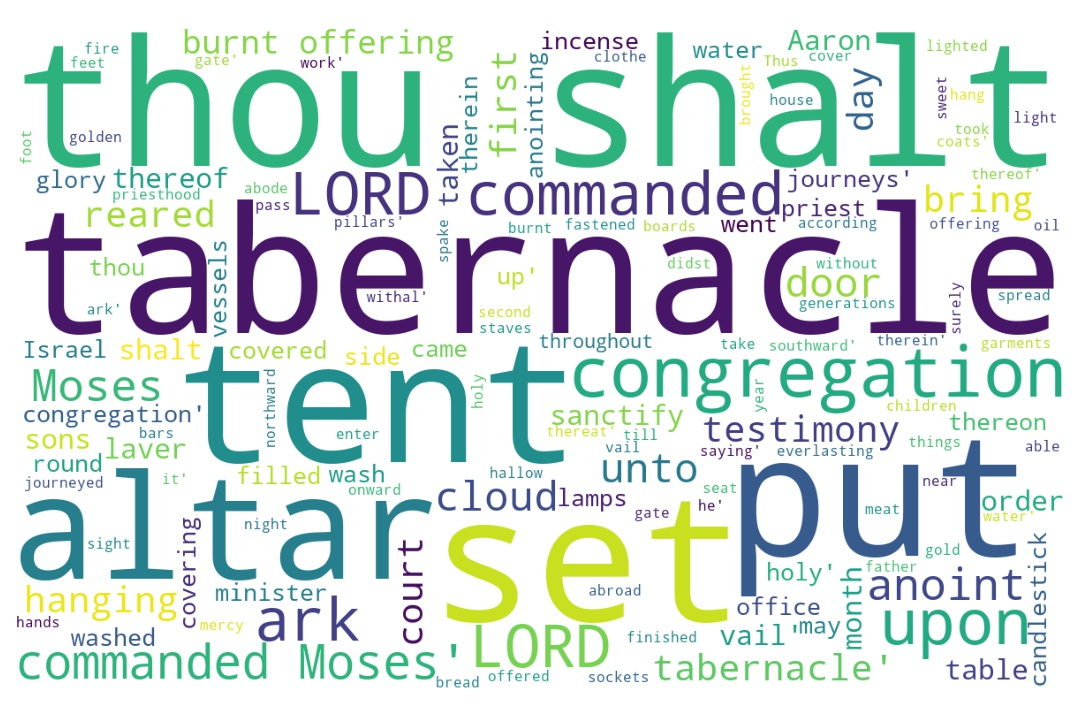
\includegraphics[width=\linewidth]{02OT-Exodus/Exodus40-WordCloud.jpg}
  \caption{Exodus 40 Word Cloud}
  \label{fig:Exodus 40 word Cloud}
\end{figure}


\marginpar{\scriptsize \centering \fcolorbox{bone}{lime}{\textbf{TABERNACLE: IOC}}\\ (Exodus 40:1-38) \begin{compactenum}[I.][8]
    \item \textbf{New Year's Day} \index[scripture]{Exodus!Exo 40:02}(Exo 40:2)  
    \item \textbf{Anointing} \index[scripture]{Exodus!Exo 40:09}\index[scripture]{Exodus!Exo 40:10}\index[scripture]{Exodus!Exo 40:11}\index[scripture]{Exodus!Exo 40:13}\index[scripture]{Exodus!Exo 40:15}(Exo 40:9, 10, 11, 13, 15) 
    \item \textbf{Needed Items} (the furniture of the tabernacle)  
    \item The \textbf{Nearness of God} \index[scripture]{Exodus!Exo 39:34}\index[scripture]{Exodus!Exo 39:35}\index[scripture]{Exodus!Exo 39:36}\index[scripture]{Exodus!Exo 39:37}\index[scripture]{Exodus!Exo 39:38}(Exo 39:34, 35, 36, 37, 38)  (the cloud)
    \item \textbf{Necessary Staff} \index[scripture]{Exodus!Exo 39:30--33}(Exo 39:30--33)  
    \item The \textbf{Numbers} 
    \begin{compactenum}[A.]
        \item The word ``tabernacle'' is used 18 times in chapter (number of bondage)
        \item The word ``Moses'' is used 13 times in chapter (number of rebellion)
    \end{compactenum}
\end{compactenum}}





\footnote{\textcolor[cmyk]{0.99998,1,0,0}{\hyperlink{TOC}{Return to end of Table of Contents.}}}\footnote{\href{https://audiobible.com/bible/exodus_40.html}{\textcolor[cmyk]{0.99998,1,0,0}{Exodus 40 Audio}}}\textcolor[cmyk]{0.99998,1,0,0}{And the LORD spake unto \fcolorbox{bone}{bone}{Moses}, saying,}
[2] \textcolor[cmyk]{0.99998,1,0,0}{On the \fcolorbox{bone}{lime}{first day} of the \fcolorbox{bone}{lime}{first month} shalt thou set up the tabernacle of the \fcolorbox{bone}{bone}{tent} of the congregation.}
[3] \textcolor[cmyk]{0.99998,1,0,0}{And thou shalt \fcolorbox{bone}{bone}{put} therein the ark of the testimony, and cover the ark with the vail.}
[4] \textcolor[cmyk]{0.99998,1,0,0}{And thou shalt bring in the table, and set in order the things that are to be set in order upon it; and thou shalt bring in the candlestick, and light the lamps thereof.}
[5] \textcolor[cmyk]{0.99998,1,0,0}{And thou shalt set the altar of gold for the incense before the ark of the testimony, and \fcolorbox{bone}{bone}{put} the hanging of the door to the tabernacle.}
[6] \textcolor[cmyk]{0.99998,1,0,0}{And thou shalt set the altar of the burnt offering before the door of the tabernacle of the \fcolorbox{bone}{bone}{tent} of the congregation.}
[7] \textcolor[cmyk]{0.99998,1,0,0}{And thou shalt set the laver between the \fcolorbox{bone}{bone}{tent} of the congregation and the altar, and shalt \fcolorbox{bone}{bone}{put} water therein.}
[8] \textcolor[cmyk]{0.99998,1,0,0}{And thou shalt set up the court round about, and hang up the hanging at the court gate.}
[9] \textcolor[cmyk]{0.99998,1,0,0}{And thou shalt take the \fcolorbox{bone}{lime}{anointing oil}, and anoint the tabernacle, and all that \emph{is} therein, and shalt hallow it, and all the vessels thereof: and it shall be holy.}
[10] \textcolor[cmyk]{0.99998,1,0,0}{And thou shalt anoint the altar of the burnt offering, and all his vessels, and sanctify the altar: and it shall be an altar most holy.}
[11] \textcolor[cmyk]{0.99998,1,0,0}{And thou shalt anoint the laver and his foot, and sanctify it.}
[12] \textcolor[cmyk]{0.99998,1,0,0}{And thou shalt bring Aaron and his sons unto the door of the tabernacle of the congregation, and wash them with water.}
[13] \textcolor[cmyk]{0.99998,1,0,0}{And thou shalt \fcolorbox{bone}{bone}{put} upon Aaron the holy garments, and anoint him, and sanctify him; that he may minister unto me in the priest's office.}
[14] \textcolor[cmyk]{0.99998,1,0,0}{And thou shalt bring his sons, and clothe them with coats:}
[15] \textcolor[cmyk]{0.99998,1,0,0}{And thou shalt anoint them, as thou didst anoint their father, that they may minister unto me in the priest's office: for their anointing shall surely be an everlasting priesthood throughout their generations.}
[16] \textcolor[cmyk]{0.99998,1,0,0}{Thus did \fcolorbox{bone}{bone}{Moses}: according to all that the LORD commanded him, so did he.}\\
\\
\P \textcolor[cmyk]{0.99998,1,0,0}{And it came to pass in the first month in the second year, on the first \emph{day} of the month, \emph{that} the tabernacle was reared up.}
[18] \textcolor[cmyk]{0.99998,1,0,0}{And \fcolorbox{bone}{bone}{Moses} reared up the tabernacle, and fastened his sockets, and set up the boards thereof, and \fcolorbox{bone}{bone}{put} in the bars thereof, and reared up his pillars.}
[19] \textcolor[cmyk]{0.99998,1,0,0}{And he spread abroad the \fcolorbox{bone}{bone}{tent} over the tabernacle, and \fcolorbox{bone}{bone}{put} the covering of the \fcolorbox{bone}{bone}{tent} above upon it; as the LORD commanded \fcolorbox{bone}{bone}{Moses}.}\\
\\
\P \textcolor[cmyk]{0.99998,1,0,0}{And he took and \fcolorbox{bone}{bone}{put} the testimony into the ark, and set the staves on the ark, and \fcolorbox{bone}{bone}{put} the mercy seat above upon the ark:}
[21] \textcolor[cmyk]{0.99998,1,0,0}{And he brought the ark into the tabernacle, and set up the vail of the covering, and covered the ark of the testimony; as the LORD commanded \fcolorbox{bone}{bone}{Moses}.}\\
\\
\P \textcolor[cmyk]{0.99998,1,0,0}{And he \fcolorbox{bone}{bone}{put} the table in the \fcolorbox{bone}{bone}{tent} of the congregation, upon the side of the tabernacle northward, without the vail.}
[23] \textcolor[cmyk]{0.99998,1,0,0}{And he set the bread in order upon it before the LORD; as the LORD had commanded \fcolorbox{bone}{bone}{Moses}.}\\
\\
\P \textcolor[cmyk]{0.99998,1,0,0}{And he \fcolorbox{bone}{bone}{put} the candlestick in the \fcolorbox{bone}{bone}{tent} of the congregation, over against the table, on the side of the tabernacle southward.}
[25] \textcolor[cmyk]{0.99998,1,0,0}{And he lighted the lamps before the LORD; as the LORD commanded \fcolorbox{bone}{bone}{Moses}.}\\
\\
\P \textcolor[cmyk]{0.99998,1,0,0}{And he \fcolorbox{bone}{bone}{put} the golden altar in the \fcolorbox{bone}{bone}{tent} of the congregation before the vail:}
[27] \textcolor[cmyk]{0.99998,1,0,0}{And he burnt sweet incense thereon; as the LORD commanded \fcolorbox{bone}{bone}{Moses}.}\\
\\
\P \textcolor[cmyk]{0.99998,1,0,0}{And he set up the hanging \emph{at} the door of the tabernacle.}
[29] \textcolor[cmyk]{0.99998,1,0,0}{And he \fcolorbox{bone}{bone}{put} the altar of burnt offering \emph{by} the door of the tabernacle of the \fcolorbox{bone}{bone}{tent} of the congregation, and offered upon it the burnt offering and the meat offering; as the LORD commanded \fcolorbox{bone}{bone}{Moses}.}\\
\\
\P \textcolor[cmyk]{0.99998,1,0,0}{And he set the laver between the \fcolorbox{bone}{bone}{tent} of the congregation and the altar, and \fcolorbox{bone}{bone}{put} water there, to wash \emph{withal}.}
[31] \textcolor[cmyk]{0.99998,1,0,0}{And \fcolorbox{bone}{bone}{Moses} and Aaron and his sons washed their hands and their feet thereat:}
[32] \textcolor[cmyk]{0.99998,1,0,0}{When they went into the \fcolorbox{bone}{bone}{tent} of the congregation, and when they came near unto the altar, they washed; as the LORD commanded \fcolorbox{bone}{bone}{Moses}.}
[33] \textcolor[cmyk]{0.99998,1,0,0}{And he reared up the court round about the tabernacle and the altar, and set up the hanging of the court gate. So \fcolorbox{bone}{bone}{Moses} finished the work.}\\
\\
\P \textcolor[cmyk]{0.99998,1,0,0}{Then \fcolorbox{bone}{lime}{a cloud} covered the \fcolorbox{bone}{bone}{tent} of the congregation, and the glory of the LORD filled the tabernacle.}
[35] \textcolor[cmyk]{0.99998,1,0,0}{And \fcolorbox{bone}{bone}{Moses} was not able to enter into the \fcolorbox{bone}{bone}{tent} of the congregation, because \fcolorbox{bone}{lime}{the cloud} abode thereon, and the glory of the LORD filled the tabernacle.}
[36] \textcolor[cmyk]{0.99998,1,0,0}{And when \fcolorbox{bone}{lime}{the cloud} was taken up from over the tabernacle, the children of Israel went onward in all their journeys:}
[37] \textcolor[cmyk]{0.99998,1,0,0}{But if \fcolorbox{bone}{lime}{the cloud} were not taken up, then they journeyed not till the day that it was taken up.}
[38] \textcolor[cmyk]{0.99998,1,0,0}{For \fcolorbox{bone}{lime}{the cloud} of the LORD \emph{was} upon the tabernacle by day, and fire was on it by night, in the sight of all the house of Israel, throughout all their journeys.}
%\index[NWIV]{7!Exodus!Exo 40:1}\index[AWIP]{And!Exodus!Exo 40:1}\index[AWIP]{the!Exodus!Exo 40:1}\index[AWIP]{LORD!Exodus!Exo 40:1}\index[AWIP]{spake!Exodus!Exo 40:1}\index[AWIP]{unto!Exodus!Exo 40:1}\index[AWIP]{Moses!Exodus!Exo 40:1}\index[AWIP]{saying!Exodus!Exo 40:1}

\index[NWIV]{20!Exodus!Exo 40:2}\index[AWIP]{On!Exodus!Exo 40:2}\index[AWIP]{the!Exodus!Exo 40:2}\index[AWIP]{the!Exodus!Exo 40:2 (2)}\index[AWIP]{the!Exodus!Exo 40:2 (3)}\index[AWIP]{the!Exodus!Exo 40:2 (4)}\index[AWIP]{the!Exodus!Exo 40:2 (5)}\index[AWIP]{first!Exodus!Exo 40:2}\index[AWIP]{first!Exodus!Exo 40:2 (2)}\index[AWIP]{day!Exodus!Exo 40:2}\index[AWIP]{of!Exodus!Exo 40:2}\index[AWIP]{of!Exodus!Exo 40:2 (2)}\index[AWIP]{of!Exodus!Exo 40:2 (3)}\index[AWIP]{month!Exodus!Exo 40:2}\index[AWIP]{shalt!Exodus!Exo 40:2}\index[AWIP]{thou!Exodus!Exo 40:2}\index[AWIP]{set!Exodus!Exo 40:2}\index[AWIP]{up!Exodus!Exo 40:2}\index[AWIP]{tabernacle!Exodus!Exo 40:2}\index[AWIP]{tent!Exodus!Exo 40:2}\index[AWIP]{congregation!Exodus!Exo 40:2}

\index[NWIV]{17!Exodus!Exo 40:3}\index[AWIP]{And!Exodus!Exo 40:3}\index[AWIP]{thou!Exodus!Exo 40:3}\index[AWIP]{shalt!Exodus!Exo 40:3}\index[AWIP]{put!Exodus!Exo 40:3}\index[AWIP]{therein!Exodus!Exo 40:3}\index[AWIP]{the!Exodus!Exo 40:3}\index[AWIP]{the!Exodus!Exo 40:3 (2)}\index[AWIP]{the!Exodus!Exo 40:3 (3)}\index[AWIP]{the!Exodus!Exo 40:3 (4)}\index[AWIP]{ark!Exodus!Exo 40:3}\index[AWIP]{ark!Exodus!Exo 40:3 (2)}\index[AWIP]{of!Exodus!Exo 40:3}\index[AWIP]{testimony!Exodus!Exo 40:3}\index[AWIP]{and!Exodus!Exo 40:3}\index[AWIP]{cover!Exodus!Exo 40:3}\index[AWIP]{with!Exodus!Exo 40:3}\index[AWIP]{vail!Exodus!Exo 40:3}

\index[NWIV]{34!Exodus!Exo 40:4}\index[AWIP]{And!Exodus!Exo 40:4}\index[AWIP]{thou!Exodus!Exo 40:4}\index[AWIP]{thou!Exodus!Exo 40:4 (2)}\index[AWIP]{shalt!Exodus!Exo 40:4}\index[AWIP]{shalt!Exodus!Exo 40:4 (2)}\index[AWIP]{bring!Exodus!Exo 40:4}\index[AWIP]{bring!Exodus!Exo 40:4 (2)}\index[AWIP]{in!Exodus!Exo 40:4}\index[AWIP]{in!Exodus!Exo 40:4 (2)}\index[AWIP]{in!Exodus!Exo 40:4 (3)}\index[AWIP]{in!Exodus!Exo 40:4 (4)}\index[AWIP]{the!Exodus!Exo 40:4}\index[AWIP]{the!Exodus!Exo 40:4 (2)}\index[AWIP]{the!Exodus!Exo 40:4 (3)}\index[AWIP]{the!Exodus!Exo 40:4 (4)}\index[AWIP]{table!Exodus!Exo 40:4}\index[AWIP]{and!Exodus!Exo 40:4}\index[AWIP]{and!Exodus!Exo 40:4 (2)}\index[AWIP]{and!Exodus!Exo 40:4 (3)}\index[AWIP]{set!Exodus!Exo 40:4}\index[AWIP]{set!Exodus!Exo 40:4 (2)}\index[AWIP]{order!Exodus!Exo 40:4}\index[AWIP]{order!Exodus!Exo 40:4 (2)}\index[AWIP]{things!Exodus!Exo 40:4}\index[AWIP]{that!Exodus!Exo 40:4}\index[AWIP]{are!Exodus!Exo 40:4}\index[AWIP]{to!Exodus!Exo 40:4}\index[AWIP]{be!Exodus!Exo 40:4}\index[AWIP]{upon!Exodus!Exo 40:4}\index[AWIP]{it!Exodus!Exo 40:4}\index[AWIP]{candlestick!Exodus!Exo 40:4}\index[AWIP]{light!Exodus!Exo 40:4}\index[AWIP]{lamps!Exodus!Exo 40:4}\index[AWIP]{thereof!Exodus!Exo 40:4}

\index[NWIV]{27!Exodus!Exo 40:5}\index[AWIP]{And!Exodus!Exo 40:5}\index[AWIP]{thou!Exodus!Exo 40:5}\index[AWIP]{shalt!Exodus!Exo 40:5}\index[AWIP]{set!Exodus!Exo 40:5}\index[AWIP]{the!Exodus!Exo 40:5}\index[AWIP]{the!Exodus!Exo 40:5 (2)}\index[AWIP]{the!Exodus!Exo 40:5 (3)}\index[AWIP]{the!Exodus!Exo 40:5 (4)}\index[AWIP]{the!Exodus!Exo 40:5 (5)}\index[AWIP]{the!Exodus!Exo 40:5 (6)}\index[AWIP]{the!Exodus!Exo 40:5 (7)}\index[AWIP]{altar!Exodus!Exo 40:5}\index[AWIP]{of!Exodus!Exo 40:5}\index[AWIP]{of!Exodus!Exo 40:5 (2)}\index[AWIP]{of!Exodus!Exo 40:5 (3)}\index[AWIP]{gold!Exodus!Exo 40:5}\index[AWIP]{for!Exodus!Exo 40:5}\index[AWIP]{incense!Exodus!Exo 40:5}\index[AWIP]{before!Exodus!Exo 40:5}\index[AWIP]{ark!Exodus!Exo 40:5}\index[AWIP]{testimony!Exodus!Exo 40:5}\index[AWIP]{and!Exodus!Exo 40:5}\index[AWIP]{put!Exodus!Exo 40:5}\index[AWIP]{hanging!Exodus!Exo 40:5}\index[AWIP]{door!Exodus!Exo 40:5}\index[AWIP]{to!Exodus!Exo 40:5}\index[AWIP]{tabernacle!Exodus!Exo 40:5}

\index[NWIV]{22!Exodus!Exo 40:6}\index[AWIP]{And!Exodus!Exo 40:6}\index[AWIP]{thou!Exodus!Exo 40:6}\index[AWIP]{shalt!Exodus!Exo 40:6}\index[AWIP]{set!Exodus!Exo 40:6}\index[AWIP]{the!Exodus!Exo 40:6}\index[AWIP]{the!Exodus!Exo 40:6 (2)}\index[AWIP]{the!Exodus!Exo 40:6 (3)}\index[AWIP]{the!Exodus!Exo 40:6 (4)}\index[AWIP]{the!Exodus!Exo 40:6 (5)}\index[AWIP]{the!Exodus!Exo 40:6 (6)}\index[AWIP]{altar!Exodus!Exo 40:6}\index[AWIP]{of!Exodus!Exo 40:6}\index[AWIP]{of!Exodus!Exo 40:6 (2)}\index[AWIP]{of!Exodus!Exo 40:6 (3)}\index[AWIP]{of!Exodus!Exo 40:6 (4)}\index[AWIP]{burnt!Exodus!Exo 40:6}\index[AWIP]{offering!Exodus!Exo 40:6}\index[AWIP]{before!Exodus!Exo 40:6}\index[AWIP]{door!Exodus!Exo 40:6}\index[AWIP]{tabernacle!Exodus!Exo 40:6}\index[AWIP]{tent!Exodus!Exo 40:6}\index[AWIP]{congregation!Exodus!Exo 40:6}

\index[NWIV]{20!Exodus!Exo 40:7}\index[AWIP]{And!Exodus!Exo 40:7}\index[AWIP]{thou!Exodus!Exo 40:7}\index[AWIP]{shalt!Exodus!Exo 40:7}\index[AWIP]{shalt!Exodus!Exo 40:7 (2)}\index[AWIP]{set!Exodus!Exo 40:7}\index[AWIP]{the!Exodus!Exo 40:7}\index[AWIP]{the!Exodus!Exo 40:7 (2)}\index[AWIP]{the!Exodus!Exo 40:7 (3)}\index[AWIP]{the!Exodus!Exo 40:7 (4)}\index[AWIP]{laver!Exodus!Exo 40:7}\index[AWIP]{between!Exodus!Exo 40:7}\index[AWIP]{tent!Exodus!Exo 40:7}\index[AWIP]{of!Exodus!Exo 40:7}\index[AWIP]{congregation!Exodus!Exo 40:7}\index[AWIP]{and!Exodus!Exo 40:7}\index[AWIP]{and!Exodus!Exo 40:7 (2)}\index[AWIP]{altar!Exodus!Exo 40:7}\index[AWIP]{put!Exodus!Exo 40:7}\index[AWIP]{water!Exodus!Exo 40:7}\index[AWIP]{therein!Exodus!Exo 40:7}

\index[NWIV]{18!Exodus!Exo 40:8}\index[AWIP]{And!Exodus!Exo 40:8}\index[AWIP]{thou!Exodus!Exo 40:8}\index[AWIP]{shalt!Exodus!Exo 40:8}\index[AWIP]{set!Exodus!Exo 40:8}\index[AWIP]{up!Exodus!Exo 40:8}\index[AWIP]{up!Exodus!Exo 40:8 (2)}\index[AWIP]{the!Exodus!Exo 40:8}\index[AWIP]{the!Exodus!Exo 40:8 (2)}\index[AWIP]{the!Exodus!Exo 40:8 (3)}\index[AWIP]{court!Exodus!Exo 40:8}\index[AWIP]{court!Exodus!Exo 40:8 (2)}\index[AWIP]{round!Exodus!Exo 40:8}\index[AWIP]{about!Exodus!Exo 40:8}\index[AWIP]{and!Exodus!Exo 40:8}\index[AWIP]{hang!Exodus!Exo 40:8}\index[AWIP]{hanging!Exodus!Exo 40:8}\index[AWIP]{at!Exodus!Exo 40:8}\index[AWIP]{gate!Exodus!Exo 40:8}

\index[NWIV]{30!Exodus!Exo 40:9}\index[AWIP]{And!Exodus!Exo 40:9}\index[AWIP]{thou!Exodus!Exo 40:9}\index[AWIP]{shalt!Exodus!Exo 40:9}\index[AWIP]{shalt!Exodus!Exo 40:9 (2)}\index[AWIP]{take!Exodus!Exo 40:9}\index[AWIP]{the!Exodus!Exo 40:9}\index[AWIP]{the!Exodus!Exo 40:9 (2)}\index[AWIP]{the!Exodus!Exo 40:9 (3)}\index[AWIP]{anointing!Exodus!Exo 40:9}\index[AWIP]{oil!Exodus!Exo 40:9}\index[AWIP]{and!Exodus!Exo 40:9}\index[AWIP]{and!Exodus!Exo 40:9 (2)}\index[AWIP]{and!Exodus!Exo 40:9 (3)}\index[AWIP]{and!Exodus!Exo 40:9 (4)}\index[AWIP]{and!Exodus!Exo 40:9 (5)}\index[AWIP]{anoint!Exodus!Exo 40:9}\index[AWIP]{tabernacle!Exodus!Exo 40:9}\index[AWIP]{all!Exodus!Exo 40:9}\index[AWIP]{all!Exodus!Exo 40:9 (2)}\index[AWIP]{that!Exodus!Exo 40:9}\index[AWIP]{\emph{is}!Exodus!Exo 40:9}\index[AWIP]{therein!Exodus!Exo 40:9}\index[AWIP]{hallow!Exodus!Exo 40:9}\index[AWIP]{it!Exodus!Exo 40:9}\index[AWIP]{it!Exodus!Exo 40:9 (2)}\index[AWIP]{vessels!Exodus!Exo 40:9}\index[AWIP]{thereof!Exodus!Exo 40:9}\index[AWIP]{shall!Exodus!Exo 40:9}\index[AWIP]{be!Exodus!Exo 40:9}\index[AWIP]{holy!Exodus!Exo 40:9}\index[AWIP]{\emph{is}!Exodus!Exo 40:9}

\index[NWIV]{26!Exodus!Exo 40:10}\index[AWIP]{And!Exodus!Exo 40:10}\index[AWIP]{thou!Exodus!Exo 40:10}\index[AWIP]{shalt!Exodus!Exo 40:10}\index[AWIP]{anoint!Exodus!Exo 40:10}\index[AWIP]{the!Exodus!Exo 40:10}\index[AWIP]{the!Exodus!Exo 40:10 (2)}\index[AWIP]{the!Exodus!Exo 40:10 (3)}\index[AWIP]{altar!Exodus!Exo 40:10}\index[AWIP]{altar!Exodus!Exo 40:10 (2)}\index[AWIP]{altar!Exodus!Exo 40:10 (3)}\index[AWIP]{of!Exodus!Exo 40:10}\index[AWIP]{burnt!Exodus!Exo 40:10}\index[AWIP]{offering!Exodus!Exo 40:10}\index[AWIP]{and!Exodus!Exo 40:10}\index[AWIP]{and!Exodus!Exo 40:10 (2)}\index[AWIP]{and!Exodus!Exo 40:10 (3)}\index[AWIP]{all!Exodus!Exo 40:10}\index[AWIP]{his!Exodus!Exo 40:10}\index[AWIP]{vessels!Exodus!Exo 40:10}\index[AWIP]{sanctify!Exodus!Exo 40:10}\index[AWIP]{it!Exodus!Exo 40:10}\index[AWIP]{shall!Exodus!Exo 40:10}\index[AWIP]{be!Exodus!Exo 40:10}\index[AWIP]{an!Exodus!Exo 40:10}\index[AWIP]{most!Exodus!Exo 40:10}\index[AWIP]{holy!Exodus!Exo 40:10}

\index[NWIV]{12!Exodus!Exo 40:11}\index[AWIP]{And!Exodus!Exo 40:11}\index[AWIP]{thou!Exodus!Exo 40:11}\index[AWIP]{shalt!Exodus!Exo 40:11}\index[AWIP]{anoint!Exodus!Exo 40:11}\index[AWIP]{the!Exodus!Exo 40:11}\index[AWIP]{laver!Exodus!Exo 40:11}\index[AWIP]{and!Exodus!Exo 40:11}\index[AWIP]{and!Exodus!Exo 40:11 (2)}\index[AWIP]{his!Exodus!Exo 40:11}\index[AWIP]{foot!Exodus!Exo 40:11}\index[AWIP]{sanctify!Exodus!Exo 40:11}\index[AWIP]{it!Exodus!Exo 40:11}

\index[NWIV]{22!Exodus!Exo 40:12}\index[AWIP]{And!Exodus!Exo 40:12}\index[AWIP]{thou!Exodus!Exo 40:12}\index[AWIP]{shalt!Exodus!Exo 40:12}\index[AWIP]{bring!Exodus!Exo 40:12}\index[AWIP]{Aaron!Exodus!Exo 40:12}\index[AWIP]{and!Exodus!Exo 40:12}\index[AWIP]{and!Exodus!Exo 40:12 (2)}\index[AWIP]{his!Exodus!Exo 40:12}\index[AWIP]{sons!Exodus!Exo 40:12}\index[AWIP]{unto!Exodus!Exo 40:12}\index[AWIP]{the!Exodus!Exo 40:12}\index[AWIP]{the!Exodus!Exo 40:12 (2)}\index[AWIP]{the!Exodus!Exo 40:12 (3)}\index[AWIP]{door!Exodus!Exo 40:12}\index[AWIP]{of!Exodus!Exo 40:12}\index[AWIP]{of!Exodus!Exo 40:12 (2)}\index[AWIP]{tabernacle!Exodus!Exo 40:12}\index[AWIP]{congregation!Exodus!Exo 40:12}\index[AWIP]{wash!Exodus!Exo 40:12}\index[AWIP]{them!Exodus!Exo 40:12}\index[AWIP]{with!Exodus!Exo 40:12}\index[AWIP]{water!Exodus!Exo 40:12}

\index[NWIV]{25!Exodus!Exo 40:13}\index[AWIP]{And!Exodus!Exo 40:13}\index[AWIP]{thou!Exodus!Exo 40:13}\index[AWIP]{shalt!Exodus!Exo 40:13}\index[AWIP]{put!Exodus!Exo 40:13}\index[AWIP]{upon!Exodus!Exo 40:13}\index[AWIP]{Aaron!Exodus!Exo 40:13}\index[AWIP]{the!Exodus!Exo 40:13}\index[AWIP]{the!Exodus!Exo 40:13 (2)}\index[AWIP]{holy!Exodus!Exo 40:13}\index[AWIP]{garments!Exodus!Exo 40:13}\index[AWIP]{and!Exodus!Exo 40:13}\index[AWIP]{and!Exodus!Exo 40:13 (2)}\index[AWIP]{anoint!Exodus!Exo 40:13}\index[AWIP]{him!Exodus!Exo 40:13}\index[AWIP]{him!Exodus!Exo 40:13 (2)}\index[AWIP]{sanctify!Exodus!Exo 40:13}\index[AWIP]{that!Exodus!Exo 40:13}\index[AWIP]{he!Exodus!Exo 40:13}\index[AWIP]{may!Exodus!Exo 40:13}\index[AWIP]{minister!Exodus!Exo 40:13}\index[AWIP]{unto!Exodus!Exo 40:13}\index[AWIP]{me!Exodus!Exo 40:13}\index[AWIP]{in!Exodus!Exo 40:13}\index[AWIP]{priest's!Exodus!Exo 40:13}\index[AWIP]{office!Exodus!Exo 40:13}

\index[NWIV]{11!Exodus!Exo 40:14}\index[AWIP]{And!Exodus!Exo 40:14}\index[AWIP]{thou!Exodus!Exo 40:14}\index[AWIP]{shalt!Exodus!Exo 40:14}\index[AWIP]{bring!Exodus!Exo 40:14}\index[AWIP]{his!Exodus!Exo 40:14}\index[AWIP]{sons!Exodus!Exo 40:14}\index[AWIP]{and!Exodus!Exo 40:14}\index[AWIP]{clothe!Exodus!Exo 40:14}\index[AWIP]{them!Exodus!Exo 40:14}\index[AWIP]{with!Exodus!Exo 40:14}\index[AWIP]{coats!Exodus!Exo 40:14}

\index[NWIV]{33!Exodus!Exo 40:15}\index[AWIP]{And!Exodus!Exo 40:15}\index[AWIP]{thou!Exodus!Exo 40:15}\index[AWIP]{thou!Exodus!Exo 40:15 (2)}\index[AWIP]{shalt!Exodus!Exo 40:15}\index[AWIP]{anoint!Exodus!Exo 40:15}\index[AWIP]{anoint!Exodus!Exo 40:15 (2)}\index[AWIP]{them!Exodus!Exo 40:15}\index[AWIP]{as!Exodus!Exo 40:15}\index[AWIP]{didst!Exodus!Exo 40:15}\index[AWIP]{their!Exodus!Exo 40:15}\index[AWIP]{their!Exodus!Exo 40:15 (2)}\index[AWIP]{their!Exodus!Exo 40:15 (3)}\index[AWIP]{father!Exodus!Exo 40:15}\index[AWIP]{that!Exodus!Exo 40:15}\index[AWIP]{they!Exodus!Exo 40:15}\index[AWIP]{may!Exodus!Exo 40:15}\index[AWIP]{minister!Exodus!Exo 40:15}\index[AWIP]{unto!Exodus!Exo 40:15}\index[AWIP]{me!Exodus!Exo 40:15}\index[AWIP]{in!Exodus!Exo 40:15}\index[AWIP]{the!Exodus!Exo 40:15}\index[AWIP]{priest's!Exodus!Exo 40:15}\index[AWIP]{office!Exodus!Exo 40:15}\index[AWIP]{for!Exodus!Exo 40:15}\index[AWIP]{anointing!Exodus!Exo 40:15}\index[AWIP]{shall!Exodus!Exo 40:15}\index[AWIP]{surely!Exodus!Exo 40:15}\index[AWIP]{be!Exodus!Exo 40:15}\index[AWIP]{an!Exodus!Exo 40:15}\index[AWIP]{everlasting!Exodus!Exo 40:15}\index[AWIP]{priesthood!Exodus!Exo 40:15}\index[AWIP]{throughout!Exodus!Exo 40:15}\index[AWIP]{generations!Exodus!Exo 40:15}

\index[NWIV]{14!Exodus!Exo 40:16}\index[AWIP]{Thus!Exodus!Exo 40:16}\index[AWIP]{did!Exodus!Exo 40:16}\index[AWIP]{did!Exodus!Exo 40:16 (2)}\index[AWIP]{Moses!Exodus!Exo 40:16}\index[AWIP]{according!Exodus!Exo 40:16}\index[AWIP]{to!Exodus!Exo 40:16}\index[AWIP]{all!Exodus!Exo 40:16}\index[AWIP]{that!Exodus!Exo 40:16}\index[AWIP]{the!Exodus!Exo 40:16}\index[AWIP]{LORD!Exodus!Exo 40:16}\index[AWIP]{commanded!Exodus!Exo 40:16}\index[AWIP]{him!Exodus!Exo 40:16}\index[AWIP]{so!Exodus!Exo 40:16}\index[AWIP]{he!Exodus!Exo 40:16}

\index[NWIV]{26!Exodus!Exo 40:17}\index[AWIP]{And!Exodus!Exo 40:17}\index[AWIP]{it!Exodus!Exo 40:17}\index[AWIP]{came!Exodus!Exo 40:17}\index[AWIP]{to!Exodus!Exo 40:17}\index[AWIP]{pass!Exodus!Exo 40:17}\index[AWIP]{in!Exodus!Exo 40:17}\index[AWIP]{in!Exodus!Exo 40:17 (2)}\index[AWIP]{the!Exodus!Exo 40:17}\index[AWIP]{the!Exodus!Exo 40:17 (2)}\index[AWIP]{the!Exodus!Exo 40:17 (3)}\index[AWIP]{the!Exodus!Exo 40:17 (4)}\index[AWIP]{the!Exodus!Exo 40:17 (5)}\index[AWIP]{first!Exodus!Exo 40:17}\index[AWIP]{first!Exodus!Exo 40:17 (2)}\index[AWIP]{month!Exodus!Exo 40:17}\index[AWIP]{month!Exodus!Exo 40:17 (2)}\index[AWIP]{second!Exodus!Exo 40:17}\index[AWIP]{year!Exodus!Exo 40:17}\index[AWIP]{on!Exodus!Exo 40:17}\index[AWIP]{\emph{day}!Exodus!Exo 40:17}\index[AWIP]{of!Exodus!Exo 40:17}\index[AWIP]{\emph{that}!Exodus!Exo 40:17}\index[AWIP]{tabernacle!Exodus!Exo 40:17}\index[AWIP]{was!Exodus!Exo 40:17}\index[AWIP]{reared!Exodus!Exo 40:17}\index[AWIP]{up!Exodus!Exo 40:17}\index[AWIP]{\emph{day}!Exodus!Exo 40:17}\index[AWIP]{\emph{that}!Exodus!Exo 40:17}

\index[NWIV]{27!Exodus!Exo 40:18}\index[AWIP]{And!Exodus!Exo 40:18}\index[AWIP]{Moses!Exodus!Exo 40:18}\index[AWIP]{reared!Exodus!Exo 40:18}\index[AWIP]{reared!Exodus!Exo 40:18 (2)}\index[AWIP]{up!Exodus!Exo 40:18}\index[AWIP]{up!Exodus!Exo 40:18 (2)}\index[AWIP]{up!Exodus!Exo 40:18 (3)}\index[AWIP]{the!Exodus!Exo 40:18}\index[AWIP]{the!Exodus!Exo 40:18 (2)}\index[AWIP]{the!Exodus!Exo 40:18 (3)}\index[AWIP]{tabernacle!Exodus!Exo 40:18}\index[AWIP]{and!Exodus!Exo 40:18}\index[AWIP]{and!Exodus!Exo 40:18 (2)}\index[AWIP]{and!Exodus!Exo 40:18 (3)}\index[AWIP]{and!Exodus!Exo 40:18 (4)}\index[AWIP]{fastened!Exodus!Exo 40:18}\index[AWIP]{his!Exodus!Exo 40:18}\index[AWIP]{his!Exodus!Exo 40:18 (2)}\index[AWIP]{sockets!Exodus!Exo 40:18}\index[AWIP]{set!Exodus!Exo 40:18}\index[AWIP]{boards!Exodus!Exo 40:18}\index[AWIP]{thereof!Exodus!Exo 40:18}\index[AWIP]{thereof!Exodus!Exo 40:18 (2)}\index[AWIP]{put!Exodus!Exo 40:18}\index[AWIP]{in!Exodus!Exo 40:18}\index[AWIP]{bars!Exodus!Exo 40:18}\index[AWIP]{pillars!Exodus!Exo 40:18}

\index[NWIV]{24!Exodus!Exo 40:19}\index[AWIP]{And!Exodus!Exo 40:19}\index[AWIP]{he!Exodus!Exo 40:19}\index[AWIP]{spread!Exodus!Exo 40:19}\index[AWIP]{abroad!Exodus!Exo 40:19}\index[AWIP]{the!Exodus!Exo 40:19}\index[AWIP]{the!Exodus!Exo 40:19 (2)}\index[AWIP]{the!Exodus!Exo 40:19 (3)}\index[AWIP]{the!Exodus!Exo 40:19 (4)}\index[AWIP]{the!Exodus!Exo 40:19 (5)}\index[AWIP]{tent!Exodus!Exo 40:19}\index[AWIP]{tent!Exodus!Exo 40:19 (2)}\index[AWIP]{over!Exodus!Exo 40:19}\index[AWIP]{tabernacle!Exodus!Exo 40:19}\index[AWIP]{and!Exodus!Exo 40:19}\index[AWIP]{put!Exodus!Exo 40:19}\index[AWIP]{covering!Exodus!Exo 40:19}\index[AWIP]{of!Exodus!Exo 40:19}\index[AWIP]{above!Exodus!Exo 40:19}\index[AWIP]{upon!Exodus!Exo 40:19}\index[AWIP]{it!Exodus!Exo 40:19}\index[AWIP]{as!Exodus!Exo 40:19}\index[AWIP]{LORD!Exodus!Exo 40:19}\index[AWIP]{commanded!Exodus!Exo 40:19}\index[AWIP]{Moses!Exodus!Exo 40:19}

\index[NWIV]{26!Exodus!Exo 40:20}\index[AWIP]{And!Exodus!Exo 40:20}\index[AWIP]{he!Exodus!Exo 40:20}\index[AWIP]{took!Exodus!Exo 40:20}\index[AWIP]{and!Exodus!Exo 40:20}\index[AWIP]{and!Exodus!Exo 40:20 (2)}\index[AWIP]{and!Exodus!Exo 40:20 (3)}\index[AWIP]{put!Exodus!Exo 40:20}\index[AWIP]{put!Exodus!Exo 40:20 (2)}\index[AWIP]{the!Exodus!Exo 40:20}\index[AWIP]{the!Exodus!Exo 40:20 (2)}\index[AWIP]{the!Exodus!Exo 40:20 (3)}\index[AWIP]{the!Exodus!Exo 40:20 (4)}\index[AWIP]{the!Exodus!Exo 40:20 (5)}\index[AWIP]{the!Exodus!Exo 40:20 (6)}\index[AWIP]{testimony!Exodus!Exo 40:20}\index[AWIP]{into!Exodus!Exo 40:20}\index[AWIP]{ark!Exodus!Exo 40:20}\index[AWIP]{ark!Exodus!Exo 40:20 (2)}\index[AWIP]{ark!Exodus!Exo 40:20 (3)}\index[AWIP]{set!Exodus!Exo 40:20}\index[AWIP]{staves!Exodus!Exo 40:20}\index[AWIP]{on!Exodus!Exo 40:20}\index[AWIP]{mercy!Exodus!Exo 40:20}\index[AWIP]{seat!Exodus!Exo 40:20}\index[AWIP]{above!Exodus!Exo 40:20}\index[AWIP]{upon!Exodus!Exo 40:20}

\index[NWIV]{28!Exodus!Exo 40:21}\index[AWIP]{And!Exodus!Exo 40:21}\index[AWIP]{he!Exodus!Exo 40:21}\index[AWIP]{brought!Exodus!Exo 40:21}\index[AWIP]{the!Exodus!Exo 40:21}\index[AWIP]{the!Exodus!Exo 40:21 (2)}\index[AWIP]{the!Exodus!Exo 40:21 (3)}\index[AWIP]{the!Exodus!Exo 40:21 (4)}\index[AWIP]{the!Exodus!Exo 40:21 (5)}\index[AWIP]{the!Exodus!Exo 40:21 (6)}\index[AWIP]{the!Exodus!Exo 40:21 (7)}\index[AWIP]{ark!Exodus!Exo 40:21}\index[AWIP]{ark!Exodus!Exo 40:21 (2)}\index[AWIP]{into!Exodus!Exo 40:21}\index[AWIP]{tabernacle!Exodus!Exo 40:21}\index[AWIP]{and!Exodus!Exo 40:21}\index[AWIP]{and!Exodus!Exo 40:21 (2)}\index[AWIP]{set!Exodus!Exo 40:21}\index[AWIP]{up!Exodus!Exo 40:21}\index[AWIP]{vail!Exodus!Exo 40:21}\index[AWIP]{of!Exodus!Exo 40:21}\index[AWIP]{of!Exodus!Exo 40:21 (2)}\index[AWIP]{covering!Exodus!Exo 40:21}\index[AWIP]{covered!Exodus!Exo 40:21}\index[AWIP]{testimony!Exodus!Exo 40:21}\index[AWIP]{as!Exodus!Exo 40:21}\index[AWIP]{LORD!Exodus!Exo 40:21}\index[AWIP]{commanded!Exodus!Exo 40:21}\index[AWIP]{Moses!Exodus!Exo 40:21}

\index[NWIV]{21!Exodus!Exo 40:22}\index[AWIP]{And!Exodus!Exo 40:22}\index[AWIP]{he!Exodus!Exo 40:22}\index[AWIP]{put!Exodus!Exo 40:22}\index[AWIP]{the!Exodus!Exo 40:22}\index[AWIP]{the!Exodus!Exo 40:22 (2)}\index[AWIP]{the!Exodus!Exo 40:22 (3)}\index[AWIP]{the!Exodus!Exo 40:22 (4)}\index[AWIP]{the!Exodus!Exo 40:22 (5)}\index[AWIP]{the!Exodus!Exo 40:22 (6)}\index[AWIP]{table!Exodus!Exo 40:22}\index[AWIP]{in!Exodus!Exo 40:22}\index[AWIP]{tent!Exodus!Exo 40:22}\index[AWIP]{of!Exodus!Exo 40:22}\index[AWIP]{of!Exodus!Exo 40:22 (2)}\index[AWIP]{congregation!Exodus!Exo 40:22}\index[AWIP]{upon!Exodus!Exo 40:22}\index[AWIP]{side!Exodus!Exo 40:22}\index[AWIP]{tabernacle!Exodus!Exo 40:22}\index[AWIP]{northward!Exodus!Exo 40:22}\index[AWIP]{without!Exodus!Exo 40:22}\index[AWIP]{vail!Exodus!Exo 40:22}

\index[NWIV]{18!Exodus!Exo 40:23}\index[AWIP]{And!Exodus!Exo 40:23}\index[AWIP]{he!Exodus!Exo 40:23}\index[AWIP]{set!Exodus!Exo 40:23}\index[AWIP]{the!Exodus!Exo 40:23}\index[AWIP]{the!Exodus!Exo 40:23 (2)}\index[AWIP]{the!Exodus!Exo 40:23 (3)}\index[AWIP]{bread!Exodus!Exo 40:23}\index[AWIP]{in!Exodus!Exo 40:23}\index[AWIP]{order!Exodus!Exo 40:23}\index[AWIP]{upon!Exodus!Exo 40:23}\index[AWIP]{it!Exodus!Exo 40:23}\index[AWIP]{before!Exodus!Exo 40:23}\index[AWIP]{LORD!Exodus!Exo 40:23}\index[AWIP]{LORD!Exodus!Exo 40:23 (2)}\index[AWIP]{as!Exodus!Exo 40:23}\index[AWIP]{had!Exodus!Exo 40:23}\index[AWIP]{commanded!Exodus!Exo 40:23}\index[AWIP]{Moses!Exodus!Exo 40:23}

\index[NWIV]{22!Exodus!Exo 40:24}\index[AWIP]{And!Exodus!Exo 40:24}\index[AWIP]{he!Exodus!Exo 40:24}\index[AWIP]{put!Exodus!Exo 40:24}\index[AWIP]{the!Exodus!Exo 40:24}\index[AWIP]{the!Exodus!Exo 40:24 (2)}\index[AWIP]{the!Exodus!Exo 40:24 (3)}\index[AWIP]{the!Exodus!Exo 40:24 (4)}\index[AWIP]{the!Exodus!Exo 40:24 (5)}\index[AWIP]{the!Exodus!Exo 40:24 (6)}\index[AWIP]{candlestick!Exodus!Exo 40:24}\index[AWIP]{in!Exodus!Exo 40:24}\index[AWIP]{tent!Exodus!Exo 40:24}\index[AWIP]{of!Exodus!Exo 40:24}\index[AWIP]{of!Exodus!Exo 40:24 (2)}\index[AWIP]{congregation!Exodus!Exo 40:24}\index[AWIP]{over!Exodus!Exo 40:24}\index[AWIP]{against!Exodus!Exo 40:24}\index[AWIP]{table!Exodus!Exo 40:24}\index[AWIP]{on!Exodus!Exo 40:24}\index[AWIP]{side!Exodus!Exo 40:24}\index[AWIP]{tabernacle!Exodus!Exo 40:24}\index[AWIP]{southward!Exodus!Exo 40:24}

\index[NWIV]{13!Exodus!Exo 40:25}\index[AWIP]{And!Exodus!Exo 40:25}\index[AWIP]{he!Exodus!Exo 40:25}\index[AWIP]{lighted!Exodus!Exo 40:25}\index[AWIP]{the!Exodus!Exo 40:25}\index[AWIP]{the!Exodus!Exo 40:25 (2)}\index[AWIP]{the!Exodus!Exo 40:25 (3)}\index[AWIP]{lamps!Exodus!Exo 40:25}\index[AWIP]{before!Exodus!Exo 40:25}\index[AWIP]{LORD!Exodus!Exo 40:25}\index[AWIP]{LORD!Exodus!Exo 40:25 (2)}\index[AWIP]{as!Exodus!Exo 40:25}\index[AWIP]{commanded!Exodus!Exo 40:25}\index[AWIP]{Moses!Exodus!Exo 40:25}

\index[NWIV]{15!Exodus!Exo 40:26}\index[AWIP]{And!Exodus!Exo 40:26}\index[AWIP]{he!Exodus!Exo 40:26}\index[AWIP]{put!Exodus!Exo 40:26}\index[AWIP]{the!Exodus!Exo 40:26}\index[AWIP]{the!Exodus!Exo 40:26 (2)}\index[AWIP]{the!Exodus!Exo 40:26 (3)}\index[AWIP]{the!Exodus!Exo 40:26 (4)}\index[AWIP]{golden!Exodus!Exo 40:26}\index[AWIP]{altar!Exodus!Exo 40:26}\index[AWIP]{in!Exodus!Exo 40:26}\index[AWIP]{tent!Exodus!Exo 40:26}\index[AWIP]{of!Exodus!Exo 40:26}\index[AWIP]{congregation!Exodus!Exo 40:26}\index[AWIP]{before!Exodus!Exo 40:26}\index[AWIP]{vail!Exodus!Exo 40:26}

\index[NWIV]{11!Exodus!Exo 40:27}\index[AWIP]{And!Exodus!Exo 40:27}\index[AWIP]{he!Exodus!Exo 40:27}\index[AWIP]{burnt!Exodus!Exo 40:27}\index[AWIP]{sweet!Exodus!Exo 40:27}\index[AWIP]{incense!Exodus!Exo 40:27}\index[AWIP]{thereon!Exodus!Exo 40:27}\index[AWIP]{as!Exodus!Exo 40:27}\index[AWIP]{the!Exodus!Exo 40:27}\index[AWIP]{LORD!Exodus!Exo 40:27}\index[AWIP]{commanded!Exodus!Exo 40:27}\index[AWIP]{Moses!Exodus!Exo 40:27}

\index[NWIV]{12!Exodus!Exo 40:28}\index[AWIP]{And!Exodus!Exo 40:28}\index[AWIP]{he!Exodus!Exo 40:28}\index[AWIP]{set!Exodus!Exo 40:28}\index[AWIP]{up!Exodus!Exo 40:28}\index[AWIP]{the!Exodus!Exo 40:28}\index[AWIP]{the!Exodus!Exo 40:28 (2)}\index[AWIP]{the!Exodus!Exo 40:28 (3)}\index[AWIP]{hanging!Exodus!Exo 40:28}\index[AWIP]{\emph{at}!Exodus!Exo 40:28}\index[AWIP]{door!Exodus!Exo 40:28}\index[AWIP]{of!Exodus!Exo 40:28}\index[AWIP]{tabernacle!Exodus!Exo 40:28}\index[AWIP]{\emph{at}!Exodus!Exo 40:28}

\index[NWIV]{36!Exodus!Exo 40:29}\index[AWIP]{And!Exodus!Exo 40:29}\index[AWIP]{he!Exodus!Exo 40:29}\index[AWIP]{put!Exodus!Exo 40:29}\index[AWIP]{the!Exodus!Exo 40:29}\index[AWIP]{the!Exodus!Exo 40:29 (2)}\index[AWIP]{the!Exodus!Exo 40:29 (3)}\index[AWIP]{the!Exodus!Exo 40:29 (4)}\index[AWIP]{the!Exodus!Exo 40:29 (5)}\index[AWIP]{the!Exodus!Exo 40:29 (6)}\index[AWIP]{the!Exodus!Exo 40:29 (7)}\index[AWIP]{the!Exodus!Exo 40:29 (8)}\index[AWIP]{altar!Exodus!Exo 40:29}\index[AWIP]{of!Exodus!Exo 40:29}\index[AWIP]{of!Exodus!Exo 40:29 (2)}\index[AWIP]{of!Exodus!Exo 40:29 (3)}\index[AWIP]{of!Exodus!Exo 40:29 (4)}\index[AWIP]{burnt!Exodus!Exo 40:29}\index[AWIP]{burnt!Exodus!Exo 40:29 (2)}\index[AWIP]{offering!Exodus!Exo 40:29}\index[AWIP]{offering!Exodus!Exo 40:29 (2)}\index[AWIP]{offering!Exodus!Exo 40:29 (3)}\index[AWIP]{\emph{by}!Exodus!Exo 40:29}\index[AWIP]{door!Exodus!Exo 40:29}\index[AWIP]{tabernacle!Exodus!Exo 40:29}\index[AWIP]{tent!Exodus!Exo 40:29}\index[AWIP]{congregation!Exodus!Exo 40:29}\index[AWIP]{and!Exodus!Exo 40:29}\index[AWIP]{and!Exodus!Exo 40:29 (2)}\index[AWIP]{offered!Exodus!Exo 40:29}\index[AWIP]{upon!Exodus!Exo 40:29}\index[AWIP]{it!Exodus!Exo 40:29}\index[AWIP]{meat!Exodus!Exo 40:29}\index[AWIP]{as!Exodus!Exo 40:29}\index[AWIP]{LORD!Exodus!Exo 40:29}\index[AWIP]{commanded!Exodus!Exo 40:29}\index[AWIP]{Moses!Exodus!Exo 40:29}\index[AWIP]{\emph{by}!Exodus!Exo 40:29}

\index[NWIV]{21!Exodus!Exo 40:30}\index[AWIP]{And!Exodus!Exo 40:30}\index[AWIP]{he!Exodus!Exo 40:30}\index[AWIP]{set!Exodus!Exo 40:30}\index[AWIP]{the!Exodus!Exo 40:30}\index[AWIP]{the!Exodus!Exo 40:30 (2)}\index[AWIP]{the!Exodus!Exo 40:30 (3)}\index[AWIP]{the!Exodus!Exo 40:30 (4)}\index[AWIP]{laver!Exodus!Exo 40:30}\index[AWIP]{between!Exodus!Exo 40:30}\index[AWIP]{tent!Exodus!Exo 40:30}\index[AWIP]{of!Exodus!Exo 40:30}\index[AWIP]{congregation!Exodus!Exo 40:30}\index[AWIP]{and!Exodus!Exo 40:30}\index[AWIP]{and!Exodus!Exo 40:30 (2)}\index[AWIP]{altar!Exodus!Exo 40:30}\index[AWIP]{put!Exodus!Exo 40:30}\index[AWIP]{water!Exodus!Exo 40:30}\index[AWIP]{there!Exodus!Exo 40:30}\index[AWIP]{to!Exodus!Exo 40:30}\index[AWIP]{wash!Exodus!Exo 40:30}\index[AWIP]{\emph{withal}!Exodus!Exo 40:30}\index[AWIP]{\emph{withal}!Exodus!Exo 40:30}

\index[NWIV]{14!Exodus!Exo 40:31}\index[AWIP]{And!Exodus!Exo 40:31}\index[AWIP]{Moses!Exodus!Exo 40:31}\index[AWIP]{and!Exodus!Exo 40:31}\index[AWIP]{and!Exodus!Exo 40:31 (2)}\index[AWIP]{and!Exodus!Exo 40:31 (3)}\index[AWIP]{Aaron!Exodus!Exo 40:31}\index[AWIP]{his!Exodus!Exo 40:31}\index[AWIP]{sons!Exodus!Exo 40:31}\index[AWIP]{washed!Exodus!Exo 40:31}\index[AWIP]{their!Exodus!Exo 40:31}\index[AWIP]{their!Exodus!Exo 40:31 (2)}\index[AWIP]{hands!Exodus!Exo 40:31}\index[AWIP]{feet!Exodus!Exo 40:31}\index[AWIP]{thereat!Exodus!Exo 40:31}

\index[NWIV]{24!Exodus!Exo 40:32}\index[AWIP]{When!Exodus!Exo 40:32}\index[AWIP]{they!Exodus!Exo 40:32}\index[AWIP]{they!Exodus!Exo 40:32 (2)}\index[AWIP]{they!Exodus!Exo 40:32 (3)}\index[AWIP]{went!Exodus!Exo 40:32}\index[AWIP]{into!Exodus!Exo 40:32}\index[AWIP]{the!Exodus!Exo 40:32}\index[AWIP]{the!Exodus!Exo 40:32 (2)}\index[AWIP]{the!Exodus!Exo 40:32 (3)}\index[AWIP]{the!Exodus!Exo 40:32 (4)}\index[AWIP]{tent!Exodus!Exo 40:32}\index[AWIP]{of!Exodus!Exo 40:32}\index[AWIP]{congregation!Exodus!Exo 40:32}\index[AWIP]{and!Exodus!Exo 40:32}\index[AWIP]{when!Exodus!Exo 40:32}\index[AWIP]{came!Exodus!Exo 40:32}\index[AWIP]{near!Exodus!Exo 40:32}\index[AWIP]{unto!Exodus!Exo 40:32}\index[AWIP]{altar!Exodus!Exo 40:32}\index[AWIP]{washed!Exodus!Exo 40:32}\index[AWIP]{as!Exodus!Exo 40:32}\index[AWIP]{LORD!Exodus!Exo 40:32}\index[AWIP]{commanded!Exodus!Exo 40:32}\index[AWIP]{Moses!Exodus!Exo 40:32}

\index[NWIV]{27!Exodus!Exo 40:33}\index[AWIP]{And!Exodus!Exo 40:33}\index[AWIP]{he!Exodus!Exo 40:33}\index[AWIP]{reared!Exodus!Exo 40:33}\index[AWIP]{up!Exodus!Exo 40:33}\index[AWIP]{up!Exodus!Exo 40:33 (2)}\index[AWIP]{the!Exodus!Exo 40:33}\index[AWIP]{the!Exodus!Exo 40:33 (2)}\index[AWIP]{the!Exodus!Exo 40:33 (3)}\index[AWIP]{the!Exodus!Exo 40:33 (4)}\index[AWIP]{the!Exodus!Exo 40:33 (5)}\index[AWIP]{the!Exodus!Exo 40:33 (6)}\index[AWIP]{court!Exodus!Exo 40:33}\index[AWIP]{court!Exodus!Exo 40:33 (2)}\index[AWIP]{round!Exodus!Exo 40:33}\index[AWIP]{about!Exodus!Exo 40:33}\index[AWIP]{tabernacle!Exodus!Exo 40:33}\index[AWIP]{and!Exodus!Exo 40:33}\index[AWIP]{and!Exodus!Exo 40:33 (2)}\index[AWIP]{altar!Exodus!Exo 40:33}\index[AWIP]{set!Exodus!Exo 40:33}\index[AWIP]{hanging!Exodus!Exo 40:33}\index[AWIP]{of!Exodus!Exo 40:33}\index[AWIP]{gate!Exodus!Exo 40:33}\index[AWIP]{So!Exodus!Exo 40:33}\index[AWIP]{Moses!Exodus!Exo 40:33}\index[AWIP]{finished!Exodus!Exo 40:33}\index[AWIP]{work!Exodus!Exo 40:33}

\index[NWIV]{18!Exodus!Exo 40:34}\index[AWIP]{Then!Exodus!Exo 40:34}\index[AWIP]{a!Exodus!Exo 40:34}\index[AWIP]{cloud!Exodus!Exo 40:34}\index[AWIP]{covered!Exodus!Exo 40:34}\index[AWIP]{the!Exodus!Exo 40:34}\index[AWIP]{the!Exodus!Exo 40:34 (2)}\index[AWIP]{the!Exodus!Exo 40:34 (3)}\index[AWIP]{the!Exodus!Exo 40:34 (4)}\index[AWIP]{the!Exodus!Exo 40:34 (5)}\index[AWIP]{tent!Exodus!Exo 40:34}\index[AWIP]{of!Exodus!Exo 40:34}\index[AWIP]{of!Exodus!Exo 40:34 (2)}\index[AWIP]{congregation!Exodus!Exo 40:34}\index[AWIP]{and!Exodus!Exo 40:34}\index[AWIP]{glory!Exodus!Exo 40:34}\index[AWIP]{LORD!Exodus!Exo 40:34}\index[AWIP]{filled!Exodus!Exo 40:34}\index[AWIP]{tabernacle!Exodus!Exo 40:34}

\index[NWIV]{27!Exodus!Exo 40:35}\index[AWIP]{And!Exodus!Exo 40:35}\index[AWIP]{Moses!Exodus!Exo 40:35}\index[AWIP]{was!Exodus!Exo 40:35}\index[AWIP]{not!Exodus!Exo 40:35}\index[AWIP]{able!Exodus!Exo 40:35}\index[AWIP]{to!Exodus!Exo 40:35}\index[AWIP]{enter!Exodus!Exo 40:35}\index[AWIP]{into!Exodus!Exo 40:35}\index[AWIP]{the!Exodus!Exo 40:35}\index[AWIP]{the!Exodus!Exo 40:35 (2)}\index[AWIP]{the!Exodus!Exo 40:35 (3)}\index[AWIP]{the!Exodus!Exo 40:35 (4)}\index[AWIP]{the!Exodus!Exo 40:35 (5)}\index[AWIP]{the!Exodus!Exo 40:35 (6)}\index[AWIP]{tent!Exodus!Exo 40:35}\index[AWIP]{of!Exodus!Exo 40:35}\index[AWIP]{of!Exodus!Exo 40:35 (2)}\index[AWIP]{congregation!Exodus!Exo 40:35}\index[AWIP]{because!Exodus!Exo 40:35}\index[AWIP]{cloud!Exodus!Exo 40:35}\index[AWIP]{abode!Exodus!Exo 40:35}\index[AWIP]{thereon!Exodus!Exo 40:35}\index[AWIP]{and!Exodus!Exo 40:35}\index[AWIP]{glory!Exodus!Exo 40:35}\index[AWIP]{LORD!Exodus!Exo 40:35}\index[AWIP]{filled!Exodus!Exo 40:35}\index[AWIP]{tabernacle!Exodus!Exo 40:35}

\index[NWIV]{21!Exodus!Exo 40:36}\index[AWIP]{And!Exodus!Exo 40:36}\index[AWIP]{when!Exodus!Exo 40:36}\index[AWIP]{the!Exodus!Exo 40:36}\index[AWIP]{the!Exodus!Exo 40:36 (2)}\index[AWIP]{the!Exodus!Exo 40:36 (3)}\index[AWIP]{cloud!Exodus!Exo 40:36}\index[AWIP]{was!Exodus!Exo 40:36}\index[AWIP]{taken!Exodus!Exo 40:36}\index[AWIP]{up!Exodus!Exo 40:36}\index[AWIP]{from!Exodus!Exo 40:36}\index[AWIP]{over!Exodus!Exo 40:36}\index[AWIP]{tabernacle!Exodus!Exo 40:36}\index[AWIP]{children!Exodus!Exo 40:36}\index[AWIP]{of!Exodus!Exo 40:36}\index[AWIP]{Israel!Exodus!Exo 40:36}\index[AWIP]{went!Exodus!Exo 40:36}\index[AWIP]{onward!Exodus!Exo 40:36}\index[AWIP]{in!Exodus!Exo 40:36}\index[AWIP]{all!Exodus!Exo 40:36}\index[AWIP]{their!Exodus!Exo 40:36}\index[AWIP]{journeys!Exodus!Exo 40:36}

\index[NWIV]{20!Exodus!Exo 40:37}\index[AWIP]{But!Exodus!Exo 40:37}\index[AWIP]{if!Exodus!Exo 40:37}\index[AWIP]{the!Exodus!Exo 40:37}\index[AWIP]{the!Exodus!Exo 40:37 (2)}\index[AWIP]{cloud!Exodus!Exo 40:37}\index[AWIP]{were!Exodus!Exo 40:37}\index[AWIP]{not!Exodus!Exo 40:37}\index[AWIP]{not!Exodus!Exo 40:37 (2)}\index[AWIP]{taken!Exodus!Exo 40:37}\index[AWIP]{taken!Exodus!Exo 40:37 (2)}\index[AWIP]{up!Exodus!Exo 40:37}\index[AWIP]{up!Exodus!Exo 40:37 (2)}\index[AWIP]{then!Exodus!Exo 40:37}\index[AWIP]{they!Exodus!Exo 40:37}\index[AWIP]{journeyed!Exodus!Exo 40:37}\index[AWIP]{till!Exodus!Exo 40:37}\index[AWIP]{day!Exodus!Exo 40:37}\index[AWIP]{that!Exodus!Exo 40:37}\index[AWIP]{it!Exodus!Exo 40:37}\index[AWIP]{was!Exodus!Exo 40:37}

\index[NWIV]{32!Exodus!Exo 40:38}\index[AWIP]{For!Exodus!Exo 40:38}\index[AWIP]{the!Exodus!Exo 40:38}\index[AWIP]{the!Exodus!Exo 40:38 (2)}\index[AWIP]{the!Exodus!Exo 40:38 (3)}\index[AWIP]{the!Exodus!Exo 40:38 (4)}\index[AWIP]{the!Exodus!Exo 40:38 (5)}\index[AWIP]{cloud!Exodus!Exo 40:38}\index[AWIP]{of!Exodus!Exo 40:38}\index[AWIP]{of!Exodus!Exo 40:38 (2)}\index[AWIP]{of!Exodus!Exo 40:38 (3)}\index[AWIP]{LORD!Exodus!Exo 40:38}\index[AWIP]{\emph{was}!Exodus!Exo 40:38}\index[AWIP]{upon!Exodus!Exo 40:38}\index[AWIP]{tabernacle!Exodus!Exo 40:38}\index[AWIP]{by!Exodus!Exo 40:38}\index[AWIP]{by!Exodus!Exo 40:38 (2)}\index[AWIP]{day!Exodus!Exo 40:38}\index[AWIP]{and!Exodus!Exo 40:38}\index[AWIP]{fire!Exodus!Exo 40:38}\index[AWIP]{was!Exodus!Exo 40:38}\index[AWIP]{on!Exodus!Exo 40:38}\index[AWIP]{it!Exodus!Exo 40:38}\index[AWIP]{night!Exodus!Exo 40:38}\index[AWIP]{in!Exodus!Exo 40:38}\index[AWIP]{sight!Exodus!Exo 40:38}\index[AWIP]{all!Exodus!Exo 40:38}\index[AWIP]{all!Exodus!Exo 40:38 (2)}\index[AWIP]{house!Exodus!Exo 40:38}\index[AWIP]{Israel!Exodus!Exo 40:38}\index[AWIP]{throughout!Exodus!Exo 40:38}\index[AWIP]{their!Exodus!Exo 40:38}\index[AWIP]{journeys!Exodus!Exo 40:38}\index[AWIP]{\emph{was}!Exodus!Exo 40:38}


%\section{Exodus 40 Outlines}

\subsection{My Outlines}

\subsubsection{Tabernacle: IOC}
\index[speaker]{Keith Anthony!Exodus 40 (Tabernacle: IOC)}
\index[series]{Exodus (Keith Anthony)!Exodus 40 (Tabernacle: IOC)}
\index[date]{2017/01/30!Exodus 40 (Tabernacle: IOC) (Keith Anthony)}
%\textbf{Introduction: }The chapter is a narrative on the presentation and reaction to God and his commands.
\begin{compactenum}[I.][8]
    \item \textbf{New Year's Day} \index[scripture]{Exodus!Exo 40:02}(Exodus 40:2)  
    \item \textbf{Anointing} \index[scripture]{Exodus!Exo 40:09}\index[scripture]{Exodus!Exo 40:10}\index[scripture]{Exodus!Exo 40:11}\index[scripture]{Exodus!Exo 40:13}\index[scripture]{Exodus!Exo 40:15}(Exodus 40:9, 10, 11, 13, 15) 
    \item \textbf{Needed Items} (the furniture of the tabernacle)  
    \item The \textbf{Nearness of God} \index[scripture]{Exodus!Exo 39:34}\index[scripture]{Exodus!Exo 39:35}\index[scripture]{Exodus!Exo 39:36}\index[scripture]{Exodus!Exo 39:37}\index[scripture]{Exodus!Exo 39:38}(Exodus 39:34, 35, 36, 37, 38)  (the cloud)
    \item \textbf{Necessary Staff} \index[scripture]{Exodus!Exo 39:30--33}(Exodus 39:30--33)  
    \item The \textbf{Numbers} 
    \begin{compactenum}[A.]
        \item The word ``tabernacle'' is used 18 times in chapter (number of bondage)
        \item The word ``Moses'' is used 13 times in chapter (number of rebellion)
    \end{compactenum}
\end{compactenum}

%\subsection{Outlines from Others}

%\section{Exodus 40 Comments}

\subsection{Numeric Nuggets}
\textbf{13: } Exodus 39:35 has 13 words. The words ``Moses,'' ``tent,'' and ``put'' are used 13 times in the chapter. Exodus 40:25 has 13 words.


%\subsection{Exodus 40 Repeated Phrases}


%%%%%%%%%%
%%%%%%%%%%
\normalsize
 
\begin{center}
\begin{longtable}{|c|c|}
\caption[Exodus 40 Repeated Phrases]{Exodus 40 Repeated Phrases}\label{table:Repeated Phrases Exodus 40} \\
\hline \multicolumn{1}{|c|}{\textbf{Phrase}} & \multicolumn{1}{c|}{\textbf{Frequency}} \\ \hline 
\endfirsthead
 
\multicolumn{2}{c}
{{\bfseries \tablename\ \thetable{} -- continued from previous page}} \\  
\hline \multicolumn{1}{|c|}{\textbf{Phrase}} & \multicolumn{1}{c|}{\textbf{Frequency}} \\ \hline 
\endhead
 
\hline \multicolumn{2}{c}{{ }} \\ \hline
\endfoot 
of the & 35\\ \hline 
the tabernacle & 18\\ \hline 
the LORD & 14\\ \hline 
thou shalt & 14\\ \hline 
the tent & 13\\ \hline 
And thou & 13\\ \hline 
And thou shalt & 13\\ \hline 
And he & 13\\ \hline 
of the congregation & 12\\ \hline 
the congregation & 12\\ \hline 
the tent of & 11\\ \hline 
the tent of the & 11\\ \hline 
the tent of the congregation & 11\\ \hline 
tent of & 11\\ \hline 
tent of the & 11\\ \hline 
tent of the congregation & 11\\ \hline 
in the & 11\\ \hline 
up the & 9\\ \hline 
the altar & 9\\ \hline 
the ark & 8\\ \hline 
put the & 8\\ \hline 
the LORD commanded & 7\\ \hline 
LORD commanded & 7\\ \hline 
as the & 7\\ \hline 
as the LORD & 7\\ \hline 
commanded Moses & 7\\ \hline 
set up & 6\\ \hline 
set up the & 6\\ \hline 
set the & 6\\ \hline 
and put & 6\\ \hline 
of the tabernacle & 6\\ \hline 
of the congregation and & 6\\ \hline 
the congregation and & 6\\ \hline 
congregation and & 6\\ \hline 
and the & 6\\ \hline 
as the LORD commanded & 6\\ \hline 
as the LORD commanded Moses & 6\\ \hline 
the LORD commanded Moses & 6\\ \hline 
LORD commanded Moses & 6\\ \hline 
and set & 5\\ \hline 
before the & 5\\ \hline 
the door & 5\\ \hline 
the tent of the congregation and & 5\\ \hline 
tent of the congregation and & 5\\ \hline 
the tabernacle and & 5\\ \hline 
tabernacle and & 5\\ \hline 
the first & 4\\ \hline 
the tabernacle of & 4\\ \hline 
the tabernacle of the & 4\\ \hline 
tabernacle of & 4\\ \hline 
tabernacle of the & 4\\ \hline 
of the tent & 4\\ \hline 
the testimony & 4\\ \hline 
the vail & 4\\ \hline 
thou shalt bring & 4\\ \hline 
shalt bring & 4\\ \hline 
upon it & 4\\ \hline 
And thou shalt set & 4\\ \hline 
thou shalt set & 4\\ \hline 
shalt set & 4\\ \hline 
the altar of & 4\\ \hline 
altar of & 4\\ \hline 
and put the & 4\\ \hline 
the hanging & 4\\ \hline 
burnt offering & 4\\ \hline 
the door of & 4\\ \hline 
the door of the & 4\\ \hline 
the door of the tabernacle & 4\\ \hline 
door of & 4\\ \hline 
door of the & 4\\ \hline 
door of the tabernacle & 4\\ \hline 
the altar and & 4\\ \hline 
altar and & 4\\ \hline 
the court & 4\\ \hline 
reared up & 4\\ \hline 
into the & 4\\ \hline 
And he put & 4\\ \hline 
And he put the & 4\\ \hline 
he put & 4\\ \hline 
he put the & 4\\ \hline 
the cloud & 4\\ \hline 
the tabernacle of the tent & 3\\ \hline 
the tabernacle of the tent of & 3\\ \hline 
the tabernacle of the tent of the & 3\\ \hline 
the tabernacle of the tent of the congregation & 3\\ \hline 
tabernacle of the tent & 3\\ \hline 
tabernacle of the tent of & 3\\ \hline 
tabernacle of the tent of the & 3\\ \hline 
tabernacle of the tent of the congregation & 3\\ \hline 
of the tent of & 3\\ \hline 
of the tent of the & 3\\ \hline 
of the tent of the congregation & 3\\ \hline 
shalt put & 3\\ \hline 
the ark of & 3\\ \hline 
the ark of the & 3\\ \hline 
the ark of the testimony & 3\\ \hline 
ark of & 3\\ \hline 
ark of the & 3\\ \hline 
ark of the testimony & 3\\ \hline 
of the testimony & 3\\ \hline 
And thou shalt bring & 3\\ \hline 
the table & 3\\ \hline 
in order & 3\\ \hline 
And thou shalt set the & 3\\ \hline 
thou shalt set the & 3\\ \hline 
shalt set the & 3\\ \hline 
the burnt & 3\\ \hline 
the burnt offering & 3\\ \hline 
the door of the tabernacle of & 3\\ \hline 
the door of the tabernacle of the & 3\\ \hline 
door of the tabernacle of & 3\\ \hline 
door of the tabernacle of the & 3\\ \hline 
of the tabernacle of & 3\\ \hline 
of the tabernacle of the & 3\\ \hline 
the laver & 3\\ \hline 
the tent of the congregation and the & 3\\ \hline 
tent of the congregation and the & 3\\ \hline 
of the congregation and the & 3\\ \hline 
the congregation and the & 3\\ \hline 
congregation and the & 3\\ \hline 
and the altar & 3\\ \hline 
and the altar and & 3\\ \hline 
up the hanging & 3\\ \hline 
anoint the & 3\\ \hline 
and all & 3\\ \hline 
thereof and & 3\\ \hline 
And thou shalt anoint & 3\\ \hline 
thou shalt anoint & 3\\ \hline 
shalt anoint & 3\\ \hline 
and sanctify & 3\\ \hline 
and his & 3\\ \hline 
his sons & 3\\ \hline 
on the & 3\\ \hline 
And Moses & 3\\ \hline 
and set up & 3\\ \hline 
and set up the & 3\\ \hline 
upon the & 3\\ \hline 
in the tent & 3\\ \hline 
in the tent of & 3\\ \hline 
in the tent of the & 3\\ \hline 
in the tent of the congregation & 3\\ \hline 
And he set & 3\\ \hline 
he set & 3\\ \hline 
of the LORD & 3\\ \hline 
taken up & 3\\ \hline 
\end{longtable}
\end{center}



%%%%%%%%%%
%%%%%%%%%%



%\section{Exodus 40 Statistics}


%%%%%%%%%%%%%%%%%%%%%%%%%%%
%%%%% Word Statistics
%%%%%%%%%%%%%%%%%%%%%%%%%%


\normalsize



\subsection{Chapter Word Statistics}


%%%%%%%%%%
%%%%%%%%%%
 
\begin{center}
\begin{longtable}{l|c|c|c|c}
\caption[Stats for Exodus 40]{Stats for Exodus 40} \label{table:Stats for Exodus 40} \\ 
\hline \multicolumn{1}{|c|}{\textbf{Verse(s)}} & \multicolumn{1}{|c|}{\textbf{Count}} & \multicolumn{1}{|c|}{\textbf{Unique}} & \multicolumn{1}{|c|}{\textbf{Italics}} & \multicolumn{1}{|c|}{\textbf{Uniq Italic}}  \\ \hline 
\endfirsthead
 
\multicolumn{5}{c}
{{\bfseries \tablename\ \thetable{} -- continued from previous page}} \\  
\hline \multicolumn{1}{|c|}{\textbf{Verse(s)}} & \multicolumn{1}{|c|}{\textbf{Count}} & \multicolumn{1}{|c|}{\textbf{Unique}} & \multicolumn{1}{|c|}{\textbf{Italics}} & \multicolumn{1}{|c|}{\textbf{Uniq Italic}}  \\ \hline 
\endhead
 
\hline \multicolumn{5}{|r|}{{Continued if needed}} \\ \hline
\endfoot 
1 & 7 & 7 & 0 & 0\\ \hline
2 & 20 & 13 & 0 & 0\\ \hline
3 & 17 & 13 & 0 & 0\\ \hline
4 & 34 & 21 & 0 & 0\\ \hline
5 & 27 & 19 & 0 & 0\\ \hline
6 & 22 & 14 & 0 & 0\\ \hline
7 & 20 & 15 & 0 & 0\\ \hline
8 & 18 & 14 & 0 & 0\\ \hline
9 & 30 & 21 & 1 & 1\\ \hline
10 & 26 & 20 & 0 & 0\\ \hline
11 & 12 & 11 & 0 & 0\\ \hline
12 & 22 & 18 & 0 & 0\\ \hline
13 & 25 & 22 & 0 & 0\\ \hline
14 & 11 & 11 & 0 & 0\\ \hline
15 & 33 & 29 & 0 & 0\\ \hline
16 & 14 & 13 & 0 & 0\\ \hline
17 & 26 & 19 & 2 & 2\\ \hline
18 & 27 & 17 & 0 & 0\\ \hline
19 & 24 & 19 & 0 & 0\\ \hline
20 & 26 & 16 & 0 & 0\\ \hline
21 & 28 & 19 & 0 & 0\\ \hline
22 & 21 & 15 & 0 & 0\\ \hline
23 & 18 & 15 & 0 & 0\\ \hline
24 & 22 & 16 & 0 & 0\\ \hline
25 & 13 & 10 & 0 & 0\\ \hline
26 & 15 & 12 & 0 & 0\\ \hline
27 & 11 & 11 & 0 & 0\\ \hline
28 & 12 & 10 & 1 & 1\\ \hline
29 & 36 & 22 & 1 & 1\\ \hline
30 & 21 & 17 & 1 & 1\\ \hline
31 & 14 & 11 & 0 & 0\\ \hline
32 & 24 & 19 & 0 & 0\\ \hline
33 & 27 & 19 & 0 & 0\\ \hline
34 & 18 & 13 & 0 & 0\\ \hline
35 & 27 & 21 & 0 & 0\\ \hline
36 & 21 & 19 & 0 & 0\\ \hline
37 & 20 & 16 & 0 & 0\\ \hline
38 & 32 & 24 & 1 & 1\\ \hline
\hline \hline
Total & 821 & 187 & 7 & 7



\end{longtable}
\end{center}

%%%%%%%%%%
%%%%%%%%%%
 
\subsection{Words by Frequency}

\begin{center}
\begin{longtable}{l|r}
\caption[Word Frequencies in Exodus 40]{Word Frequencies in Exodus 40} \label{table:WordsIn-Exodus-40} \\ 
\hline \multicolumn{1}{|c|}{\textbf{Word}} & \multicolumn{1}{c|}{\textbf{Frequency}} \\ \hline 
\endfirsthead
 
\multicolumn{2}{c}
{{\bfseries \tablename\ \thetable{} -- continued from previous page}} \\ 
\hline \multicolumn{1}{|c|}{\textbf{Word}} & \multicolumn{1}{c|}{\textbf{Frequency}} \\ \hline 
\endhead
 
\hline \multicolumn{2}{|r|}{{Continued if needed}} \\ \hline
\endfoot
 
\hline \hline
\endlastfoot
the & 143 \\ \hline
and & 46 \\ \hline
of & 40 \\ \hline
And & 32 \\ \hline
tabernacle & 18 \\ \hline
shalt & 17 \\ \hline
thou & 16 \\ \hline
in & 15 \\ \hline
he & 15 \\ \hline
LORD & 14 \\ \hline
set & 14 \\ \hline
up & 14 \\ \hline
Moses & 13 \\ \hline
tent & 13 \\ \hline
put & 13 \\ \hline
congregation & 12 \\ \hline
it & 11 \\ \hline
altar & 11 \\ \hline
ark & 8 \\ \hline
upon & 8 \\ \hline
as & 8 \\ \hline
commanded & 8 \\ \hline
all & 7 \\ \hline
his & 7 \\ \hline
their & 7 \\ \hline
that & 6 \\ \hline
to & 6 \\ \hline
anoint & 6 \\ \hline
unto & 5 \\ \hline
before & 5 \\ \hline
door & 5 \\ \hline
burnt & 5 \\ \hline
offering & 5 \\ \hline
they & 5 \\ \hline
was & 5 \\ \hline
cloud & 5 \\ \hline
first & 4 \\ \hline
testimony & 4 \\ \hline
vail & 4 \\ \hline
bring & 4 \\ \hline
be & 4 \\ \hline
thereof & 4 \\ \hline
hanging & 4 \\ \hline
court & 4 \\ \hline
on & 4 \\ \hline
reared & 4 \\ \hline
into & 4 \\ \hline
day & 3 \\ \hline
month & 3 \\ \hline
therein & 3 \\ \hline
with & 3 \\ \hline
table & 3 \\ \hline
order & 3 \\ \hline
laver & 3 \\ \hline
water & 3 \\ \hline
shall & 3 \\ \hline
holy & 3 \\ \hline
sanctify & 3 \\ \hline
Aaron & 3 \\ \hline
sons & 3 \\ \hline
them & 3 \\ \hline
him & 3 \\ \hline
over & 3 \\ \hline
not & 3 \\ \hline
taken & 3 \\ \hline
candlestick & 2 \\ \hline
lamps & 2 \\ \hline
for & 2 \\ \hline
incense & 2 \\ \hline
between & 2 \\ \hline
round & 2 \\ \hline
about & 2 \\ \hline
gate & 2 \\ \hline
anointing & 2 \\ \hline
vessels & 2 \\ \hline
an & 2 \\ \hline
wash & 2 \\ \hline
may & 2 \\ \hline
minister & 2 \\ \hline
me & 2 \\ \hline
priest's & 2 \\ \hline
office & 2 \\ \hline
throughout & 2 \\ \hline
did & 2 \\ \hline
came & 2 \\ \hline
covering & 2 \\ \hline
above & 2 \\ \hline
covered & 2 \\ \hline
side & 2 \\ \hline
thereon & 2 \\ \hline
washed & 2 \\ \hline
went & 2 \\ \hline
when & 2 \\ \hline
glory & 2 \\ \hline
filled & 2 \\ \hline
Israel & 2 \\ \hline
journeys & 2 \\ \hline
by & 2 \\ \hline
spake & 1 \\ \hline
saying & 1 \\ \hline
On & 1 \\ \hline
cover & 1 \\ \hline
things & 1 \\ \hline
are & 1 \\ \hline
light & 1 \\ \hline
gold & 1 \\ \hline
hang & 1 \\ \hline
at & 1 \\ \hline
take & 1 \\ \hline
oil & 1 \\ \hline
\emph{is} & 1 \\ \hline
hallow & 1 \\ \hline
most & 1 \\ \hline
foot & 1 \\ \hline
garments & 1 \\ \hline
clothe & 1 \\ \hline
coats & 1 \\ \hline
didst & 1 \\ \hline
father & 1 \\ \hline
surely & 1 \\ \hline
everlasting & 1 \\ \hline
priesthood & 1 \\ \hline
generations & 1 \\ \hline
Thus & 1 \\ \hline
according & 1 \\ \hline
so & 1 \\ \hline
pass & 1 \\ \hline
second & 1 \\ \hline
year & 1 \\ \hline
\emph{day} & 1 \\ \hline
\emph{that} & 1 \\ \hline
fastened & 1 \\ \hline
sockets & 1 \\ \hline
boards & 1 \\ \hline
bars & 1 \\ \hline
pillars & 1 \\ \hline
spread & 1 \\ \hline
abroad & 1 \\ \hline
took & 1 \\ \hline
staves & 1 \\ \hline
mercy & 1 \\ \hline
seat & 1 \\ \hline
brought & 1 \\ \hline
northward & 1 \\ \hline
without & 1 \\ \hline
bread & 1 \\ \hline
had & 1 \\ \hline
against & 1 \\ \hline
southward & 1 \\ \hline
lighted & 1 \\ \hline
golden & 1 \\ \hline
sweet & 1 \\ \hline
\emph{at} & 1 \\ \hline
\emph{by} & 1 \\ \hline
offered & 1 \\ \hline
meat & 1 \\ \hline
there & 1 \\ \hline
\emph{withal} & 1 \\ \hline
hands & 1 \\ \hline
feet & 1 \\ \hline
thereat & 1 \\ \hline
When & 1 \\ \hline
near & 1 \\ \hline
So & 1 \\ \hline
finished & 1 \\ \hline
work & 1 \\ \hline
Then & 1 \\ \hline
a & 1 \\ \hline
able & 1 \\ \hline
enter & 1 \\ \hline
because & 1 \\ \hline
abode & 1 \\ \hline
from & 1 \\ \hline
children & 1 \\ \hline
onward & 1 \\ \hline
But & 1 \\ \hline
if & 1 \\ \hline
were & 1 \\ \hline
then & 1 \\ \hline
journeyed & 1 \\ \hline
till & 1 \\ \hline
For & 1 \\ \hline
\emph{was} & 1 \\ \hline
fire & 1 \\ \hline
night & 1 \\ \hline
sight & 1 \\ \hline
house & 1 \\ \hline
\end{longtable}
\end{center}



\normalsize



\subsection{Words Alphabetically}

\begin{center}
\begin{longtable}{l|r}
\caption[Word Alphabetically in Exodus 40]{Word Alphabetically in Exodus 40} \label{table:WordsIn-Exodus-40} \\ 
\hline \multicolumn{1}{|c|}{\textbf{Word}} & \multicolumn{1}{c|}{\textbf{Frequency}} \\ \hline 
\endfirsthead
 
\multicolumn{2}{c}
{{\bfseries \tablename\ \thetable{} -- continued from previous page}} \\ 
\hline \multicolumn{1}{|c|}{\textbf{Word}} & \multicolumn{1}{c|}{\textbf{Frequency}} \\ \hline 
\endhead
 
\hline \multicolumn{2}{|r|}{{Continued if needed}} \\ \hline
\endfoot
 
\hline \hline
\endlastfoot
Aaron & 3 \\ \hline
And & 32 \\ \hline
But & 1 \\ \hline
For & 1 \\ \hline
Israel & 2 \\ \hline
LORD & 14 \\ \hline
Moses & 13 \\ \hline
On & 1 \\ \hline
So & 1 \\ \hline
Then & 1 \\ \hline
Thus & 1 \\ \hline
When & 1 \\ \hline
\emph{at} & 1 \\ \hline
\emph{by} & 1 \\ \hline
\emph{day} & 1 \\ \hline
\emph{is} & 1 \\ \hline
\emph{that} & 1 \\ \hline
\emph{was} & 1 \\ \hline
\emph{withal} & 1 \\ \hline
a & 1 \\ \hline
able & 1 \\ \hline
abode & 1 \\ \hline
about & 2 \\ \hline
above & 2 \\ \hline
abroad & 1 \\ \hline
according & 1 \\ \hline
against & 1 \\ \hline
all & 7 \\ \hline
altar & 11 \\ \hline
an & 2 \\ \hline
and & 46 \\ \hline
anoint & 6 \\ \hline
anointing & 2 \\ \hline
are & 1 \\ \hline
ark & 8 \\ \hline
as & 8 \\ \hline
at & 1 \\ \hline
bars & 1 \\ \hline
be & 4 \\ \hline
because & 1 \\ \hline
before & 5 \\ \hline
between & 2 \\ \hline
boards & 1 \\ \hline
bread & 1 \\ \hline
bring & 4 \\ \hline
brought & 1 \\ \hline
burnt & 5 \\ \hline
by & 2 \\ \hline
came & 2 \\ \hline
candlestick & 2 \\ \hline
children & 1 \\ \hline
clothe & 1 \\ \hline
cloud & 5 \\ \hline
coats & 1 \\ \hline
commanded & 8 \\ \hline
congregation & 12 \\ \hline
court & 4 \\ \hline
cover & 1 \\ \hline
covered & 2 \\ \hline
covering & 2 \\ \hline
day & 3 \\ \hline
did & 2 \\ \hline
didst & 1 \\ \hline
door & 5 \\ \hline
enter & 1 \\ \hline
everlasting & 1 \\ \hline
fastened & 1 \\ \hline
father & 1 \\ \hline
feet & 1 \\ \hline
filled & 2 \\ \hline
finished & 1 \\ \hline
fire & 1 \\ \hline
first & 4 \\ \hline
foot & 1 \\ \hline
for & 2 \\ \hline
from & 1 \\ \hline
garments & 1 \\ \hline
gate & 2 \\ \hline
generations & 1 \\ \hline
glory & 2 \\ \hline
gold & 1 \\ \hline
golden & 1 \\ \hline
had & 1 \\ \hline
hallow & 1 \\ \hline
hands & 1 \\ \hline
hang & 1 \\ \hline
hanging & 4 \\ \hline
he & 15 \\ \hline
him & 3 \\ \hline
his & 7 \\ \hline
holy & 3 \\ \hline
house & 1 \\ \hline
if & 1 \\ \hline
in & 15 \\ \hline
incense & 2 \\ \hline
into & 4 \\ \hline
it & 11 \\ \hline
journeyed & 1 \\ \hline
journeys & 2 \\ \hline
lamps & 2 \\ \hline
laver & 3 \\ \hline
light & 1 \\ \hline
lighted & 1 \\ \hline
may & 2 \\ \hline
me & 2 \\ \hline
meat & 1 \\ \hline
mercy & 1 \\ \hline
minister & 2 \\ \hline
month & 3 \\ \hline
most & 1 \\ \hline
near & 1 \\ \hline
night & 1 \\ \hline
northward & 1 \\ \hline
not & 3 \\ \hline
of & 40 \\ \hline
offered & 1 \\ \hline
offering & 5 \\ \hline
office & 2 \\ \hline
oil & 1 \\ \hline
on & 4 \\ \hline
onward & 1 \\ \hline
order & 3 \\ \hline
over & 3 \\ \hline
pass & 1 \\ \hline
pillars & 1 \\ \hline
priest's & 2 \\ \hline
priesthood & 1 \\ \hline
put & 13 \\ \hline
reared & 4 \\ \hline
round & 2 \\ \hline
sanctify & 3 \\ \hline
saying & 1 \\ \hline
seat & 1 \\ \hline
second & 1 \\ \hline
set & 14 \\ \hline
shall & 3 \\ \hline
shalt & 17 \\ \hline
side & 2 \\ \hline
sight & 1 \\ \hline
so & 1 \\ \hline
sockets & 1 \\ \hline
sons & 3 \\ \hline
southward & 1 \\ \hline
spake & 1 \\ \hline
spread & 1 \\ \hline
staves & 1 \\ \hline
surely & 1 \\ \hline
sweet & 1 \\ \hline
tabernacle & 18 \\ \hline
table & 3 \\ \hline
take & 1 \\ \hline
taken & 3 \\ \hline
tent & 13 \\ \hline
testimony & 4 \\ \hline
that & 6 \\ \hline
the & 143 \\ \hline
their & 7 \\ \hline
them & 3 \\ \hline
then & 1 \\ \hline
there & 1 \\ \hline
thereat & 1 \\ \hline
therein & 3 \\ \hline
thereof & 4 \\ \hline
thereon & 2 \\ \hline
they & 5 \\ \hline
things & 1 \\ \hline
thou & 16 \\ \hline
throughout & 2 \\ \hline
till & 1 \\ \hline
to & 6 \\ \hline
took & 1 \\ \hline
unto & 5 \\ \hline
up & 14 \\ \hline
upon & 8 \\ \hline
vail & 4 \\ \hline
vessels & 2 \\ \hline
was & 5 \\ \hline
wash & 2 \\ \hline
washed & 2 \\ \hline
water & 3 \\ \hline
went & 2 \\ \hline
were & 1 \\ \hline
when & 2 \\ \hline
with & 3 \\ \hline
without & 1 \\ \hline
work & 1 \\ \hline
year & 1 \\ \hline
\end{longtable}
\end{center}



\normalsize



\subsection{Word Lengths in Chapter}
\normalsize
\begin{longtable}{l|p{3.75in}}
\caption[Words by Length in Exodus 40]{Words by Length in Exodus 40} \label{table:WordsIn-Exodus-40} \\ 
\hline \multicolumn{1}{|c|}{\textbf{Length}} & \multicolumn{1}{c|}{\textbf{Words}} \\ \hline 
\endfirsthead
 
\multicolumn{2}{c}
{{\bfseries \tablename\ \thetable{} -- continued from previous page}} \\ 
\hline \multicolumn{1}{|c|}{\textbf{Length}} & \multicolumn{1}{c|}{\textbf{Words}} \\ \hline 
\endhead
 
\hline \multicolumn{2}{|r|}{{Continued if needed}} \\ \hline
\endfoot
 
\hline \hline
\endlastfoot
1 & a \\ \hline
2 & On, of, up, in, to, be, it, at, \emph{is}, an, he, me, as, so, on, \emph{at}, \emph{by}, So, if, by \\ \hline
3 & And, the, day, set, put, ark, and, are, for, oil, all, his, him, may, did, \emph{day}, was, had, not, But, For, \emph{was} \\ \hline
4 & LORD, unto, thou, tent, with, vail, that, upon, gold, door, hang, gate, take, holy, most, foot, sons, wash, them, they, Thus, came, pass, year, \emph{that}, bars, over, took, into, seat, side, meat, feet, When, went, when, near, work, Then, able, from, were, then, till, fire \\ \hline
5 & spake, Moses, first, month, shalt, cover, bring, table, order, light, lamps, altar, burnt, laver, water, court, round, about, shall, Aaron, coats, didst, their, above, mercy, bread, sweet, there, hands, cloud, glory, enter, abode, taken, night, sight, house \\ \hline
6 & saying, things, before, anoint, hallow, office, clothe, father, surely, second, reared, boards, spread, abroad, staves, golden, \emph{withal}, washed, filled, Israel, onward \\ \hline
7 & therein, thereof, incense, hanging, between, vessels, sockets, pillars, brought, covered, without, against, lighted, thereon, offered, thereat, because \\ \hline
8 & offering, sanctify, garments, minister, priest's, fastened, covering, finished, children, journeys \\ \hline
9 & testimony, anointing, according, commanded, northward, southward, journeyed \\ \hline
10 & tabernacle, priesthood, throughout \\ \hline
11 & candlestick, everlasting, generations \\ \hline
12 & congregation \\ \hline
\end{longtable}






%%%%%%%%%%
%%%%%%%%%%
 



%%%%%%%%%%
%%%%%%%%%%
\subsection{Verses with 13 Words in Chapter}
\normalsize
\begin{longtable}{l|p{3.75in}}
\caption[Verses with 13 Words  in Exodus 40]{Verses with 13 Words  in Exodus 40} \label{table:Verses with 13 Words in-Exodus-40} \\ 
\hline \multicolumn{1}{|c|}{\textbf{Reference}} & \multicolumn{1}{c|}{\textbf{Verse}} \\ \hline 
\endfirsthead
 
\multicolumn{2}{c}
{{\bfseries \tablename\ \thetable{} -- continued from previous page}} \\ 
\hline \multicolumn{1}{|c|}{\textbf{Reference}} & \multicolumn{1}{c|}{\textbf{Verse}} \\ \hline 
\endhead
 
\hline \multicolumn{2}{|r|}{{Continued if needed}} \\ \hline
\endfoot
 
\hline \hline
\endlastfoot
Exodus 40:25 & And he lighted the lamps before the LORD; as the LORD commanded Moses. \\ \hline
\end{longtable}






%%%%%%%%%%
%%%%%%%%%%
 



%%%%%%%%%%
%%%%%%%%%%
\subsection{Verses with 18 Words in Chapter}
\normalsize
\begin{longtable}{l|p{3.75in}}
\caption[Verses with 18 Words  in Exodus 40]{Verses with 18 Words  in Exodus 40} \label{table:Verses with 18 Words in-Exodus-40} \\ 
\hline \multicolumn{1}{|c|}{\textbf{Reference}} & \multicolumn{1}{c|}{\textbf{Verse}} \\ \hline 
\endfirsthead
 
\multicolumn{2}{c}
{{\bfseries \tablename\ \thetable{} -- continued from previous page}} \\ 
\hline \multicolumn{1}{|c|}{\textbf{Reference}} & \multicolumn{1}{c|}{\textbf{Verse}} \\ \hline 
\endhead
 
\hline \multicolumn{2}{|r|}{{Continued if needed}} \\ \hline
\endfoot
 
\hline \hline
\endlastfoot
Exodus 40:8 & And thou shalt set up the court round about, and hang up the hanging at the court gate. \\ \hline
Exodus 40:23 & And he set the bread in order upon it before the LORD; as the LORD had commanded Moses. \\ \hline
Exodus 40:34 & Then a cloud covered the tent of the congregation, and the glory of the LORD filled the tabernacle. \\ \hline
\end{longtable}






%%%%%%%%%%
%%%%%%%%%%
 

\chapter{Psalm 30}

\begin{figure}
  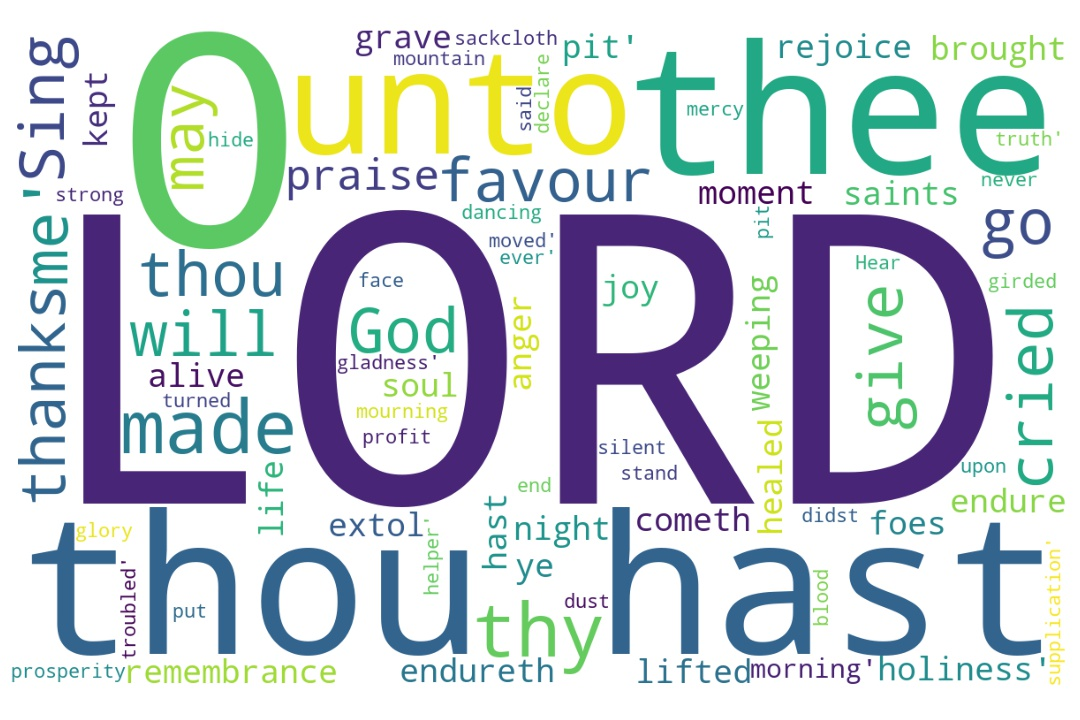
\includegraphics[width=\linewidth]{19OT-Psalms/Psalm30-WordCloud.jpg}
  \caption{Psalm 30 Word Cloud}
  \label{fig:Psalm 30 word Cloud}
\end{figure}


\marginpar{\scriptsize \centering \fcolorbox{bone}{lime}{\textbf{GOD'S FAVOUR}}\\ (Psalm 30:1--12) 
\begin{compactenum}[I.][8]
    \item David spared at the \textbf{Brink of Death} \index[scripture]{Psalms!Psa 030:03} (Psa 30:3)
    \item God's favor was David's \textbf{Basis for Deliverance} \index[scripture]{Psalms!Psa 030:05} (Psa 30:5)
    \item David's \textbf{Bad Declaration} \index[scripture]{Psalms!Psa 030:06} (Psa 30:6)
    \item David's \textbf{Better Decision}  \index[scripture]{Psalms!Psa 030:07} (Psa 30:7)
    \item David gets \textbf{Blessing instead of Dust} \index[scripture]{Psalms!Psa 030:09} (Psa 30:9)
    \item God changed David's \textbf{Bitterness into Dancing} \index[scripture]{Psalms!Psa 030:11} (Psa 30:11)
    \item David gets a \textbf{Bright Destiny} \index[scripture]{Psalms!Psa 030:12} (Psa 30:12)
\end{compactenum} }

%%%%%%%%%%%%%%%%%%%%%%%%%%%%%%%%%
%%%%%%%%%%%%%%%%%%%%%%%%%%%%%%%%%
\footnote{\textcolor[cmyk]{0.99998,1,0,0}{\hyperlink{TOC}{Return to end of Table of Contents.}}}\footnote{\href{https://www.audioverse.org/english/audiobibles/books/ENGKJV/O/Ps/1}{\textcolor[cmyk]{0.99998,1,0,0}{Psalms Audio}}}\textcolor[cmyk]{0.99998,1,0,0}{A Psalm \emph{and} Song \emph{at} the dedication of the house of David.}\\
\\
\textcolor[cmyk]{0.99998,1,0,0}{I will extol thee, O LORD; for thou hast lifted me up, and hast not made my foes to rejoice over me.}
[2] \textcolor[cmyk]{0.99998,1,0,0}{O LORD my God, I cried unto thee, and thou hast healed me.}
[3] \textcolor[cmyk]{0.99998,1,0,0}{O LORD, thou hast brought up my soul \fcolorbox{bone}{lime}{from the grave}: thou hast kept me alive, that I should not go down to the pit.}
[4] \textcolor[cmyk]{0.99998,1,0,0}{Sing unto the LORD, O ye saints of his, and give thanks at the remembrance of his holiness.}
[5] \textcolor[cmyk]{0.99998,1,0,0}{For his anger \emph{endureth} \emph{but} a moment; in \fcolorbox{bone}{lime}{his favour} \emph{is} life: weeping may endure for a night, but joy \emph{cometh} in the morning.}
[6] \textcolor[cmyk]{0.99998,1,0,0}{And in my prosperity I said, I shall \fcolorbox{bone}{lime}{never} be moved.}
[7] \textcolor[cmyk]{0.99998,1,0,0}{LORD, by \fcolorbox{bone}{lime}{thy favour} thou hast made my mountain to stand strong: thou didst hide thy face, \emph{and} I was troubled.}
[8] \textcolor[cmyk]{0.99998,1,0,0}{I \fcolorbox{bone}{lime}{cried to thee}, O LORD; and unto the LORD I made supplication.}
[9] \textcolor[cmyk]{0.99998,1,0,0}{What profit \emph{is} \emph{there} in my blood, when I go down to the pit? Shall the \fcolorbox{bone}{lime}{dust} praise thee? shall it declare thy truth?}
[10] \textcolor[cmyk]{0.99998,1,0,0}{Hear, O LORD, and have mercy upon me: LORD, be thou my helper.}
[11] \textcolor[cmyk]{0.99998,1,0,0}{Thou hast turned for me my mourning into \fcolorbox{bone}{lime}{dancing}: thou hast put off my sackcloth, and girded me with gladness;}
[12] \textcolor[cmyk]{0.99998,1,0,0}{To \fcolorbox{bone}{lime}{the end} that \emph{my} glory may sing praise to thee, and not be silent. O LORD my God, I will give thanks unto thee for ever.}
\index[NWIV]{22!Psalms!Psa 30:1}\index[AWIP]{I!Psalms!Psa 30:1}\index[AWIP]{will!Psalms!Psa 30:1}\index[AWIP]{extol!Psalms!Psa 30:1}\index[AWIP]{thee!Psalms!Psa 30:1}\index[AWIP]{O!Psalms!Psa 30:1}\index[AWIP]{LORD!Psalms!Psa 30:1}\index[AWIP]{for!Psalms!Psa 30:1}\index[AWIP]{thou!Psalms!Psa 30:1}\index[AWIP]{hast!Psalms!Psa 30:1}\index[AWIP]{hast!Psalms!Psa 30:1 (2)}\index[AWIP]{lifted!Psalms!Psa 30:1}\index[AWIP]{me!Psalms!Psa 30:1}\index[AWIP]{me!Psalms!Psa 30:1 (2)}\index[AWIP]{up!Psalms!Psa 30:1}\index[AWIP]{and!Psalms!Psa 30:1}\index[AWIP]{not!Psalms!Psa 30:1}\index[AWIP]{made!Psalms!Psa 30:1}\index[AWIP]{my!Psalms!Psa 30:1}\index[AWIP]{foes!Psalms!Psa 30:1}\index[AWIP]{to!Psalms!Psa 30:1}\index[AWIP]{rejoice!Psalms!Psa 30:1}\index[AWIP]{over!Psalms!Psa 30:1}

\index[NWIV]{13!Psalms!Psa 30:2}\index[AWIP]{O!Psalms!Psa 30:2}\index[AWIP]{LORD!Psalms!Psa 30:2}\index[AWIP]{my!Psalms!Psa 30:2}\index[AWIP]{God!Psalms!Psa 30:2}\index[AWIP]{I!Psalms!Psa 30:2}\index[AWIP]{cried!Psalms!Psa 30:2}\index[AWIP]{unto!Psalms!Psa 30:2}\index[AWIP]{thee!Psalms!Psa 30:2}\index[AWIP]{and!Psalms!Psa 30:2}\index[AWIP]{thou!Psalms!Psa 30:2}\index[AWIP]{hast!Psalms!Psa 30:2}\index[AWIP]{healed!Psalms!Psa 30:2}\index[AWIP]{me!Psalms!Psa 30:2}

\index[NWIV]{25!Psalms!Psa 30:3}\index[AWIP]{O!Psalms!Psa 30:3}\index[AWIP]{LORD!Psalms!Psa 30:3}\index[AWIP]{thou!Psalms!Psa 30:3}\index[AWIP]{thou!Psalms!Psa 30:3 (2)}\index[AWIP]{hast!Psalms!Psa 30:3}\index[AWIP]{hast!Psalms!Psa 30:3 (2)}\index[AWIP]{brought!Psalms!Psa 30:3}\index[AWIP]{up!Psalms!Psa 30:3}\index[AWIP]{my!Psalms!Psa 30:3}\index[AWIP]{soul!Psalms!Psa 30:3}\index[AWIP]{from!Psalms!Psa 30:3}\index[AWIP]{the!Psalms!Psa 30:3}\index[AWIP]{the!Psalms!Psa 30:3 (2)}\index[AWIP]{grave!Psalms!Psa 30:3}\index[AWIP]{kept!Psalms!Psa 30:3}\index[AWIP]{me!Psalms!Psa 30:3}\index[AWIP]{alive!Psalms!Psa 30:3}\index[AWIP]{that!Psalms!Psa 30:3}\index[AWIP]{I!Psalms!Psa 30:3}\index[AWIP]{should!Psalms!Psa 30:3}\index[AWIP]{not!Psalms!Psa 30:3}\index[AWIP]{go!Psalms!Psa 30:3}\index[AWIP]{down!Psalms!Psa 30:3}\index[AWIP]{to!Psalms!Psa 30:3}\index[AWIP]{pit!Psalms!Psa 30:3}

\index[NWIV]{18!Psalms!Psa 30:4}\index[AWIP]{Sing!Psalms!Psa 30:4}\index[AWIP]{unto!Psalms!Psa 30:4}\index[AWIP]{the!Psalms!Psa 30:4}\index[AWIP]{the!Psalms!Psa 30:4 (2)}\index[AWIP]{LORD!Psalms!Psa 30:4}\index[AWIP]{O!Psalms!Psa 30:4}\index[AWIP]{ye!Psalms!Psa 30:4}\index[AWIP]{saints!Psalms!Psa 30:4}\index[AWIP]{of!Psalms!Psa 30:4}\index[AWIP]{of!Psalms!Psa 30:4 (2)}\index[AWIP]{his!Psalms!Psa 30:4}\index[AWIP]{his!Psalms!Psa 30:4 (2)}\index[AWIP]{and!Psalms!Psa 30:4}\index[AWIP]{give!Psalms!Psa 30:4}\index[AWIP]{thanks!Psalms!Psa 30:4}\index[AWIP]{at!Psalms!Psa 30:4}\index[AWIP]{remembrance!Psalms!Psa 30:4}\index[AWIP]{holiness!Psalms!Psa 30:4}

\index[NWIV]{24!Psalms!Psa 30:5}\index[AWIP]{For!Psalms!Psa 30:5}\index[AWIP]{his!Psalms!Psa 30:5}\index[AWIP]{his!Psalms!Psa 30:5 (2)}\index[AWIP]{anger!Psalms!Psa 30:5}\index[AWIP]{\emph{endureth}!Psalms!Psa 30:5}\index[AWIP]{\emph{but}!Psalms!Psa 30:5}\index[AWIP]{a!Psalms!Psa 30:5}\index[AWIP]{a!Psalms!Psa 30:5 (2)}\index[AWIP]{moment!Psalms!Psa 30:5}\index[AWIP]{in!Psalms!Psa 30:5}\index[AWIP]{in!Psalms!Psa 30:5 (2)}\index[AWIP]{favour!Psalms!Psa 30:5}\index[AWIP]{\emph{is}!Psalms!Psa 30:5}\index[AWIP]{life!Psalms!Psa 30:5}\index[AWIP]{weeping!Psalms!Psa 30:5}\index[AWIP]{may!Psalms!Psa 30:5}\index[AWIP]{endure!Psalms!Psa 30:5}\index[AWIP]{for!Psalms!Psa 30:5}\index[AWIP]{night!Psalms!Psa 30:5}\index[AWIP]{but!Psalms!Psa 30:5}\index[AWIP]{joy!Psalms!Psa 30:5}\index[AWIP]{\emph{cometh}!Psalms!Psa 30:5}\index[AWIP]{the!Psalms!Psa 30:5}\index[AWIP]{morning!Psalms!Psa 30:5}\index[AWIP]{\emph{endureth}!Psalms!Psa 30:5}\index[AWIP]{\emph{but}!Psalms!Psa 30:5}\index[AWIP]{\emph{is}!Psalms!Psa 30:5}\index[AWIP]{\emph{cometh}!Psalms!Psa 30:5}

\index[NWIV]{11!Psalms!Psa 30:6}\index[AWIP]{And!Psalms!Psa 30:6}\index[AWIP]{in!Psalms!Psa 30:6}\index[AWIP]{my!Psalms!Psa 30:6}\index[AWIP]{prosperity!Psalms!Psa 30:6}\index[AWIP]{I!Psalms!Psa 30:6}\index[AWIP]{I!Psalms!Psa 30:6 (2)}\index[AWIP]{said!Psalms!Psa 30:6}\index[AWIP]{shall!Psalms!Psa 30:6}\index[AWIP]{never!Psalms!Psa 30:6}\index[AWIP]{be!Psalms!Psa 30:6}\index[AWIP]{moved!Psalms!Psa 30:6}

\index[NWIV]{21!Psalms!Psa 30:7}\index[AWIP]{LORD!Psalms!Psa 30:7}\index[AWIP]{by!Psalms!Psa 30:7}\index[AWIP]{thy!Psalms!Psa 30:7}\index[AWIP]{thy!Psalms!Psa 30:7 (2)}\index[AWIP]{favour!Psalms!Psa 30:7}\index[AWIP]{thou!Psalms!Psa 30:7}\index[AWIP]{thou!Psalms!Psa 30:7 (2)}\index[AWIP]{hast!Psalms!Psa 30:7}\index[AWIP]{made!Psalms!Psa 30:7}\index[AWIP]{my!Psalms!Psa 30:7}\index[AWIP]{mountain!Psalms!Psa 30:7}\index[AWIP]{to!Psalms!Psa 30:7}\index[AWIP]{stand!Psalms!Psa 30:7}\index[AWIP]{strong!Psalms!Psa 30:7}\index[AWIP]{didst!Psalms!Psa 30:7}\index[AWIP]{hide!Psalms!Psa 30:7}\index[AWIP]{face!Psalms!Psa 30:7}\index[AWIP]{\emph{and}!Psalms!Psa 30:7}\index[AWIP]{I!Psalms!Psa 30:7}\index[AWIP]{was!Psalms!Psa 30:7}\index[AWIP]{troubled!Psalms!Psa 30:7}\index[AWIP]{\emph{and}!Psalms!Psa 30:7}

\index[NWIV]{13!Psalms!Psa 30:8}\index[AWIP]{I!Psalms!Psa 30:8}\index[AWIP]{I!Psalms!Psa 30:8 (2)}\index[AWIP]{cried!Psalms!Psa 30:8}\index[AWIP]{to!Psalms!Psa 30:8}\index[AWIP]{thee!Psalms!Psa 30:8}\index[AWIP]{O!Psalms!Psa 30:8}\index[AWIP]{LORD!Psalms!Psa 30:8}\index[AWIP]{LORD!Psalms!Psa 30:8 (2)}\index[AWIP]{and!Psalms!Psa 30:8}\index[AWIP]{unto!Psalms!Psa 30:8}\index[AWIP]{the!Psalms!Psa 30:8}\index[AWIP]{made!Psalms!Psa 30:8}\index[AWIP]{supplication!Psalms!Psa 30:8}

\index[NWIV]{24!Psalms!Psa 30:9}\index[AWIP]{What!Psalms!Psa 30:9}\index[AWIP]{profit!Psalms!Psa 30:9}\index[AWIP]{\emph{is}!Psalms!Psa 30:9}\index[AWIP]{\emph{there}!Psalms!Psa 30:9}\index[AWIP]{in!Psalms!Psa 30:9}\index[AWIP]{my!Psalms!Psa 30:9}\index[AWIP]{blood!Psalms!Psa 30:9}\index[AWIP]{when!Psalms!Psa 30:9}\index[AWIP]{I!Psalms!Psa 30:9}\index[AWIP]{go!Psalms!Psa 30:9}\index[AWIP]{down!Psalms!Psa 30:9}\index[AWIP]{to!Psalms!Psa 30:9}\index[AWIP]{the!Psalms!Psa 30:9}\index[AWIP]{the!Psalms!Psa 30:9 (2)}\index[AWIP]{pit?!Psalms!Psa 30:9}\index[AWIP]{Shall!Psalms!Psa 30:9}\index[AWIP]{dust!Psalms!Psa 30:9}\index[AWIP]{praise!Psalms!Psa 30:9}\index[AWIP]{thee?!Psalms!Psa 30:9}\index[AWIP]{shall!Psalms!Psa 30:9}\index[AWIP]{it!Psalms!Psa 30:9}\index[AWIP]{declare!Psalms!Psa 30:9}\index[AWIP]{thy!Psalms!Psa 30:9}\index[AWIP]{truth?!Psalms!Psa 30:9}\index[AWIP]{\emph{is}!Psalms!Psa 30:9}\index[AWIP]{\emph{there}!Psalms!Psa 30:9}

\index[NWIV]{13!Psalms!Psa 30:10}\index[AWIP]{Hear!Psalms!Psa 30:10}\index[AWIP]{O!Psalms!Psa 30:10}\index[AWIP]{LORD!Psalms!Psa 30:10}\index[AWIP]{LORD!Psalms!Psa 30:10 (2)}\index[AWIP]{and!Psalms!Psa 30:10}\index[AWIP]{have!Psalms!Psa 30:10}\index[AWIP]{mercy!Psalms!Psa 30:10}\index[AWIP]{upon!Psalms!Psa 30:10}\index[AWIP]{me!Psalms!Psa 30:10}\index[AWIP]{be!Psalms!Psa 30:10}\index[AWIP]{thou!Psalms!Psa 30:10}\index[AWIP]{my!Psalms!Psa 30:10}\index[AWIP]{helper!Psalms!Psa 30:10}

\index[NWIV]{20!Psalms!Psa 30:11}\index[AWIP]{Thou!Psalms!Psa 30:11}\index[AWIP]{hast!Psalms!Psa 30:11}\index[AWIP]{hast!Psalms!Psa 30:11 (2)}\index[AWIP]{turned!Psalms!Psa 30:11}\index[AWIP]{for!Psalms!Psa 30:11}\index[AWIP]{me!Psalms!Psa 30:11}\index[AWIP]{me!Psalms!Psa 30:11 (2)}\index[AWIP]{my!Psalms!Psa 30:11}\index[AWIP]{my!Psalms!Psa 30:11 (2)}\index[AWIP]{mourning!Psalms!Psa 30:11}\index[AWIP]{into!Psalms!Psa 30:11}\index[AWIP]{dancing!Psalms!Psa 30:11}\index[AWIP]{thou!Psalms!Psa 30:11}\index[AWIP]{put!Psalms!Psa 30:11}\index[AWIP]{off!Psalms!Psa 30:11}\index[AWIP]{sackcloth!Psalms!Psa 30:11}\index[AWIP]{and!Psalms!Psa 30:11}\index[AWIP]{girded!Psalms!Psa 30:11}\index[AWIP]{with!Psalms!Psa 30:11}\index[AWIP]{gladness!Psalms!Psa 30:11}

\index[NWIV]{27!Psalms!Psa 30:12}\index[AWIP]{To!Psalms!Psa 30:12}\index[AWIP]{the!Psalms!Psa 30:12}\index[AWIP]{end!Psalms!Psa 30:12}\index[AWIP]{that!Psalms!Psa 30:12}\index[AWIP]{\emph{my}!Psalms!Psa 30:12}\index[AWIP]{glory!Psalms!Psa 30:12}\index[AWIP]{may!Psalms!Psa 30:12}\index[AWIP]{sing!Psalms!Psa 30:12}\index[AWIP]{praise!Psalms!Psa 30:12}\index[AWIP]{to!Psalms!Psa 30:12}\index[AWIP]{thee!Psalms!Psa 30:12}\index[AWIP]{thee!Psalms!Psa 30:12 (2)}\index[AWIP]{and!Psalms!Psa 30:12}\index[AWIP]{not!Psalms!Psa 30:12}\index[AWIP]{be!Psalms!Psa 30:12}\index[AWIP]{silent!Psalms!Psa 30:12}\index[AWIP]{O!Psalms!Psa 30:12}\index[AWIP]{LORD!Psalms!Psa 30:12}\index[AWIP]{my!Psalms!Psa 30:12}\index[AWIP]{God!Psalms!Psa 30:12}\index[AWIP]{I!Psalms!Psa 30:12}\index[AWIP]{will!Psalms!Psa 30:12}\index[AWIP]{give!Psalms!Psa 30:12}\index[AWIP]{thanks!Psalms!Psa 30:12}\index[AWIP]{unto!Psalms!Psa 30:12}\index[AWIP]{for!Psalms!Psa 30:12}\index[AWIP]{ever!Psalms!Psa 30:12}\index[AWIP]{\emph{my}!Psalms!Psa 30:12}

%%%%%%%%%%%%%%%%%%%%%%%%%%%%%%%%%%%%
\index[DOCTRINES]{Practicology - Strange Woman!Psalms!Psa 30:20}

\index[DOCTRINES]{Practicology - Strife!Psalms!Psa 30:33}


\section{Psalm 30 Outlines}

\subsection{My Outlines}

\subsubsection{God's Favour}
\index[speaker]{Keith Anthony!Psalm 030 (God's Favour)}
\index[series]{Psalms (Keith Anthony)!Psalm 030 (God's Favour)}
\index[date]{2014/11/02!Psalm 030 (God's Favour) (Keith Anthony)}
Introduction: The superscription for Psalm 30 reads ``A Psalm and Song at the dedication of the house of David,'' connecting it with the dedication of the site for the Temple (\index[scripture]{1 Chronicles!1Chr 21:26}1 Chronicles 21:26 and \index[scripture]{1 Chronicles!1Chr 22: 1}1 Chronicles 22:1). The psalm has three verses (\index[scripture]{Psalms!Psa 030:02}Psalm 30:2, \index[scripture]{Psalms!Psa 030:08}Psalm 30:8, and \index[scripture]{Psalms!Psa 030:10}Psalm 30:10) with 13 words, showing that despite David's sin and deep-down rebellion, God still kept His covenant with David. Instances of the number 13 typically indicate rebellion, or an opportunity to choose between rebellion or obedience, or here, repentance. Psalm 30:3 indicates that God had delivered David, at some point, from the brink of death. Some hold that Psalm 30:6-7 refers to the plague God sent in response to David's census, done against God's command (see 2 Samuel 24 and 1 Chronicles 21). Consider aspects of God's favor upon David:
\begin{compactenum}
    \item David was spared at the \textbf{Brink of Death} \index[scripture]{Psalms!Psa 030:03} (Psa 30:3)
    \item God's favor was David's \textbf{Basis for Deliverance} \index[scripture]{Psalms!Psa 030:05} (Psa 30:5)
    \item God's favor was given despite David's \textbf{Bad Declaration} - David was comfortable and secure and apparently forgot the source of all his blessings. \index[scripture]{Psalms!Psa 030:06} (Psa 30:6)
    \item God's seeming absence results in David's \textbf{Better Decision}  \index[scripture]{Psalms!Psa 030:07} (Psa 30:7)
    \item Because of God's favor David gets \textbf{Blessing instead of Dust} \index[scripture]{Psalms!Psa 030:09} (Psa 30:9)
    \item God changed David's \textbf{Bitterness into Dancing} \index[scripture]{Psalms!Psa 030:11} (Psa 30:11)
    \item Because of God's Favor, David has a \textbf{Bright Destiny} \index[scripture]{Psalms!Psa 030:12} (Psa 30:12)\\
\end{compactenum}
Do you have God's favor in your life? Do you even want it?

% made 3 (1, 7, 8)  may 2 (5, 12)  me 7 (1 (2x), 2, 3, 10, 11 (2x)) mercy 1 (10) moment 1 (5) morning 1(5) mountain 1 (7)  mourning 1 (11) moved 1 (6) my 10 (1, 2, 3, 6, 7, 9, 10, 11 (2x), 12) 
\subsection{Outlines from Others}

\section{Psalm 30 Comments}

\subsection{Numeric Nuggets}
There are 13 words in Psalm 30:2, Psalm 30:8, and Psalm 30:10.
\subsection{Psalm 30 Repeated Phrases}


%%%%%%%%%%
%%%%%%%%%%
\normalsize
 
\begin{center}
\begin{longtable}{|c|c|}
\caption[Psalm 30 Repeated Phrases]{Psalm 30 Repeated Phrases}\label{table:Repeated Phrases Psalm 30} \\
\hline \multicolumn{1}{|c|}{\textbf{Phrase}} & \multicolumn{1}{c|}{\textbf{Frequency}} \\ \hline 
\endfirsthead
 
\multicolumn{2}{c}
{{\bfseries \tablename\ \thetable{} -- continued from previous page}} \\  
\hline \multicolumn{1}{|c|}{\textbf{Phrase}} & \multicolumn{1}{c|}{\textbf{Frequency}} \\ \hline 
\endhead
 
\hline \multicolumn{2}{c}{{ }} \\ \hline
\endfoot 
O LORD & 6\\ \hline 
thou hast & 6\\ \hline 
\end{longtable}
\end{center}



%%%%%%%%%%
%%%%%%%%%%



\section{Psalm 30 Statistics}

%%%%%%%%%%%%%%%%%%%%%%%%%%%
%%%%% Word Statistics
%%%%%%%%%%%%%%%%%%%%%%%%%%


\normalsize



\subsection{Chapter Word Statistics}


%%%%%%%%%%
%%%%%%%%%%
 
\begin{center}
\begin{longtable}{l|c|c|c|c}
\caption[Stats for Psalm 30]{Stats for Psalm 30} \label{table:Stats for Psalm 30} \\ 
\hline \multicolumn{1}{|c|}{\textbf{Verse(s)}} & \multicolumn{1}{|c|}{\textbf{Count}} & \multicolumn{1}{|c|}{\textbf{Unique}} & \multicolumn{1}{|c|}{\textbf{Italics}} & \multicolumn{1}{|c|}{\textbf{Uniq Italic}}  \\ \hline 
\endfirsthead
 
\multicolumn{5}{c}
{{\bfseries \tablename\ \thetable{} -- continued from previous page}} \\  
\hline \multicolumn{1}{|c|}{\textbf{Verse(s)}} & \multicolumn{1}{|c|}{\textbf{Count}} & \multicolumn{1}{|c|}{\textbf{Unique}} & \multicolumn{1}{|c|}{\textbf{Italics}} & \multicolumn{1}{|c|}{\textbf{Uniq Italic}}  \\ \hline 
\endhead
 
\hline \multicolumn{5}{|r|}{{Continued if needed}} \\ \hline
\endfoot 
1 & 22 & 20 & 0 & 0\\ \hline
2 & 13 & 13 & 0 & 0\\ \hline
3 & 25 & 22 & 0 & 0\\ \hline
4 & 18 & 15 & 0 & 0\\ \hline
5 & 24 & 21 & 4 & 4\\ \hline
6 & 11 & 10 & 0 & 0\\ \hline
7 & 21 & 19 & 1 & 1\\ \hline
8 & 13 & 11 & 0 & 0\\ \hline
9 & 24 & 23 & 2 & 2\\ \hline
10 & 13 & 12 & 0 & 0\\ \hline
11 & 20 & 17 & 0 & 0\\ \hline
12 & 27 & 26 & 1 & 1\\ \hline
\hline \hline
Total & 231 & 117 & 8 & 7



\end{longtable}
\end{center}

%%%%%%%%%%
%%%%%%%%%%
 
\subsection{Words by Frequency}

\begin{center}
\begin{longtable}{l|r}
\caption[Word Frequencies in Psalm 30]{Word Frequencies in Psalm 30} \label{table:WordsIn-Psalm-30} \\ 
\hline \multicolumn{1}{|c|}{\textbf{Word}} & \multicolumn{1}{c|}{\textbf{Frequency}} \\ \hline 
\endfirsthead
 
\multicolumn{2}{c}
{{\bfseries \tablename\ \thetable{} -- continued from previous page}} \\ 
\hline \multicolumn{1}{|c|}{\textbf{Word}} & \multicolumn{1}{c|}{\textbf{Frequency}} \\ \hline 
\endhead
 
\hline \multicolumn{2}{|r|}{{Continued if needed}} \\ \hline
\endfoot
 
\hline \hline
\endlastfoot
I & 10 \\ \hline
LORD & 10 \\ \hline
my & 10 \\ \hline
the & 9 \\ \hline
thou & 8 \\ \hline
hast & 8 \\ \hline
O & 7 \\ \hline
me & 7 \\ \hline
and & 7 \\ \hline
thee & 6 \\ \hline
to & 6 \\ \hline
for & 4 \\ \hline
unto & 4 \\ \hline
his & 4 \\ \hline
in & 4 \\ \hline
not & 3 \\ \hline
made & 3 \\ \hline
be & 3 \\ \hline
thy & 3 \\ \hline
will & 2 \\ \hline
up & 2 \\ \hline
God & 2 \\ \hline
cried & 2 \\ \hline
that & 2 \\ \hline
go & 2 \\ \hline
down & 2 \\ \hline
pit & 2 \\ \hline
of & 2 \\ \hline
give & 2 \\ \hline
thanks & 2 \\ \hline
a & 2 \\ \hline
favour & 2 \\ \hline
\emph{is} & 2 \\ \hline
may & 2 \\ \hline
shall & 2 \\ \hline
praise & 2 \\ \hline
extol & 1 \\ \hline
lifted & 1 \\ \hline
foes & 1 \\ \hline
rejoice & 1 \\ \hline
over & 1 \\ \hline
healed & 1 \\ \hline
brought & 1 \\ \hline
soul & 1 \\ \hline
from & 1 \\ \hline
grave & 1 \\ \hline
kept & 1 \\ \hline
alive & 1 \\ \hline
should & 1 \\ \hline
Sing & 1 \\ \hline
ye & 1 \\ \hline
saints & 1 \\ \hline
at & 1 \\ \hline
remembrance & 1 \\ \hline
holiness & 1 \\ \hline
For & 1 \\ \hline
anger & 1 \\ \hline
\emph{endureth} & 1 \\ \hline
\emph{but} & 1 \\ \hline
moment & 1 \\ \hline
life & 1 \\ \hline
weeping & 1 \\ \hline
endure & 1 \\ \hline
night & 1 \\ \hline
but & 1 \\ \hline
joy & 1 \\ \hline
\emph{cometh} & 1 \\ \hline
morning & 1 \\ \hline
And & 1 \\ \hline
prosperity & 1 \\ \hline
said & 1 \\ \hline
never & 1 \\ \hline
moved & 1 \\ \hline
by & 1 \\ \hline
mountain & 1 \\ \hline
stand & 1 \\ \hline
strong & 1 \\ \hline
didst & 1 \\ \hline
hide & 1 \\ \hline
face & 1 \\ \hline
\emph{and} & 1 \\ \hline
was & 1 \\ \hline
troubled & 1 \\ \hline
supplication & 1 \\ \hline
What & 1 \\ \hline
profit & 1 \\ \hline
\emph{there} & 1 \\ \hline
blood & 1 \\ \hline
when & 1 \\ \hline
Shall & 1 \\ \hline
dust & 1 \\ \hline
it & 1 \\ \hline
declare & 1 \\ \hline
truth & 1 \\ \hline
Hear & 1 \\ \hline
have & 1 \\ \hline
mercy & 1 \\ \hline
upon & 1 \\ \hline
helper & 1 \\ \hline
Thou & 1 \\ \hline
turned & 1 \\ \hline
mourning & 1 \\ \hline
into & 1 \\ \hline
dancing & 1 \\ \hline
put & 1 \\ \hline
off & 1 \\ \hline
sackcloth & 1 \\ \hline
girded & 1 \\ \hline
with & 1 \\ \hline
gladness & 1 \\ \hline
To & 1 \\ \hline
end & 1 \\ \hline
\emph{my} & 1 \\ \hline
glory & 1 \\ \hline
sing & 1 \\ \hline
silent & 1 \\ \hline
ever & 1 \\ \hline
\end{longtable}
\end{center}



\normalsize



\subsection{Words Alphabetically}

\begin{center}
\begin{longtable}{l|r}
\caption[Word Alphabetically in Psalm 30]{Word Alphabetically in Psalm 30} \label{table:WordsIn-Psalm-30} \\ 
\hline \multicolumn{1}{|c|}{\textbf{Word}} & \multicolumn{1}{c|}{\textbf{Frequency}} \\ \hline 
\endfirsthead
 
\multicolumn{2}{c}
{{\bfseries \tablename\ \thetable{} -- continued from previous page}} \\ 
\hline \multicolumn{1}{|c|}{\textbf{Word}} & \multicolumn{1}{c|}{\textbf{Frequency}} \\ \hline 
\endhead
 
\hline \multicolumn{2}{|r|}{{Continued if needed}} \\ \hline
\endfoot
 
\hline \hline
\endlastfoot
And & 1 \\ \hline
For & 1 \\ \hline
God & 2 \\ \hline
Hear & 1 \\ \hline
I & 10 \\ \hline
LORD & 10 \\ \hline
O & 7 \\ \hline
Shall & 1 \\ \hline
Sing & 1 \\ \hline
Thou & 1 \\ \hline
To & 1 \\ \hline
What & 1 \\ \hline
\emph{and} & 1 \\ \hline
\emph{but} & 1 \\ \hline
\emph{cometh} & 1 \\ \hline
\emph{endureth} & 1 \\ \hline
\emph{is} & 2 \\ \hline
\emph{my} & 1 \\ \hline
\emph{there} & 1 \\ \hline
a & 2 \\ \hline
alive & 1 \\ \hline
and & 7 \\ \hline
anger & 1 \\ \hline
at & 1 \\ \hline
be & 3 \\ \hline
blood & 1 \\ \hline
brought & 1 \\ \hline
but & 1 \\ \hline
by & 1 \\ \hline
cried & 2 \\ \hline
dancing & 1 \\ \hline
declare & 1 \\ \hline
didst & 1 \\ \hline
down & 2 \\ \hline
dust & 1 \\ \hline
end & 1 \\ \hline
endure & 1 \\ \hline
ever & 1 \\ \hline
extol & 1 \\ \hline
face & 1 \\ \hline
favour & 2 \\ \hline
foes & 1 \\ \hline
for & 4 \\ \hline
from & 1 \\ \hline
girded & 1 \\ \hline
give & 2 \\ \hline
gladness & 1 \\ \hline
glory & 1 \\ \hline
go & 2 \\ \hline
grave & 1 \\ \hline
hast & 8 \\ \hline
have & 1 \\ \hline
healed & 1 \\ \hline
helper & 1 \\ \hline
hide & 1 \\ \hline
his & 4 \\ \hline
holiness & 1 \\ \hline
in & 4 \\ \hline
into & 1 \\ \hline
it & 1 \\ \hline
joy & 1 \\ \hline
kept & 1 \\ \hline
life & 1 \\ \hline
lifted & 1 \\ \hline
made & 3 \\ \hline
may & 2 \\ \hline
me & 7 \\ \hline
mercy & 1 \\ \hline
moment & 1 \\ \hline
morning & 1 \\ \hline
mountain & 1 \\ \hline
mourning & 1 \\ \hline
moved & 1 \\ \hline
my & 10 \\ \hline
never & 1 \\ \hline
night & 1 \\ \hline
not & 3 \\ \hline
of & 2 \\ \hline
off & 1 \\ \hline
over & 1 \\ \hline
pit & 2 \\ \hline
praise & 2 \\ \hline
profit & 1 \\ \hline
prosperity & 1 \\ \hline
put & 1 \\ \hline
rejoice & 1 \\ \hline
remembrance & 1 \\ \hline
sackcloth & 1 \\ \hline
said & 1 \\ \hline
saints & 1 \\ \hline
shall & 2 \\ \hline
should & 1 \\ \hline
silent & 1 \\ \hline
sing & 1 \\ \hline
soul & 1 \\ \hline
stand & 1 \\ \hline
strong & 1 \\ \hline
supplication & 1 \\ \hline
thanks & 2 \\ \hline
that & 2 \\ \hline
the & 9 \\ \hline
thee & 6 \\ \hline
thou & 8 \\ \hline
thy & 3 \\ \hline
to & 6 \\ \hline
troubled & 1 \\ \hline
truth & 1 \\ \hline
turned & 1 \\ \hline
unto & 4 \\ \hline
up & 2 \\ \hline
upon & 1 \\ \hline
was & 1 \\ \hline
weeping & 1 \\ \hline
when & 1 \\ \hline
will & 2 \\ \hline
with & 1 \\ \hline
ye & 1 \\ \hline
\end{longtable}
\end{center}



\normalsize



\subsection{Word Lengths in Chapter}
\normalsize
\begin{longtable}{l|p{3.75in}}
\caption[Words by Length in Psalm 30]{Words by Length in Psalm 30} \label{table:WordsIn-Psalm-30} \\ 
\hline \multicolumn{1}{|c|}{\textbf{Length}} & \multicolumn{1}{c|}{\textbf{Words}} \\ \hline 
\endfirsthead
 
\multicolumn{2}{c}
{{\bfseries \tablename\ \thetable{} -- continued from previous page}} \\ 
\hline \multicolumn{1}{|c|}{\textbf{Length}} & \multicolumn{1}{c|}{\textbf{Words}} \\ \hline 
\endhead
 
\hline \multicolumn{2}{|r|}{{Continued if needed}} \\ \hline
\endfoot
 
\hline \hline
\endlastfoot
1 & I, O, a \\ \hline
2 & me, up, my, to, go, ye, of, at, in, \emph{is}, be, by, it, To, \emph{my} \\ \hline
3 & for, and, not, God, the, pit, his, For, \emph{but}, may, but, joy, And, thy, \emph{and}, was, put, off, end \\ \hline
4 & will, thee, LORD, thou, hast, made, foes, over, unto, soul, from, kept, that, down, Sing, give, life, said, hide, face, What, when, dust, Hear, have, upon, Thou, into, with, sing, ever \\ \hline
5 & extol, cried, grave, alive, anger, night, shall, never, moved, stand, didst, \emph{there}, blood, Shall, truth, mercy, glory \\ \hline
6 & lifted, healed, should, saints, thanks, moment, favour, endure, \emph{cometh}, strong, profit, praise, helper, turned, girded, silent \\ \hline
7 & rejoice, brought, weeping, morning, declare, dancing \\ \hline
8 & holiness, \emph{endureth}, mountain, troubled, mourning, gladness \\ \hline
9 & sackcloth \\ \hline
10 & prosperity \\ \hline
11 & remembrance \\ \hline
12 & supplication \\ \hline
\end{longtable}






%%%%%%%%%%
%%%%%%%%%%
 



%%%%%%%%%%
%%%%%%%%%%
\subsection{Verses with 13 Words in Chapter}
\normalsize
\begin{longtable}{l|p{3.75in}}
\caption[Verses with 13 Words  in Psalm 30]{Verses with 13 Words  in Psalm 30} \label{table:Verses with 13 Words in-Psalm-30} \\ 
\hline \multicolumn{1}{|c|}{\textbf{Reference}} & \multicolumn{1}{c|}{\textbf{Verse}} \\ \hline 
\endfirsthead
 
\multicolumn{2}{c}
{{\bfseries \tablename\ \thetable{} -- continued from previous page}} \\ 
\hline \multicolumn{1}{|c|}{\textbf{Reference}} & \multicolumn{1}{c|}{\textbf{Verse}} \\ \hline 
\endhead
 
\hline \multicolumn{2}{|r|}{{Continued if needed}} \\ \hline
\endfoot
 
\hline \hline
\endlastfoot
Psalms 030:2 & O LORD my God, I cried unto thee, and thou hast healed me. \\ \hline
Psalms 030:8 & I cried to thee, O LORD; and unto the LORD I made supplication. \\ \hline
Psalms 030:10 & Hear, O LORD, and have mercy upon me: LORD, be thou my helper. \\ \hline
\end{longtable}






%%%%%%%%%%
%%%%%%%%%%
 



%%%%%%%%%%
%%%%%%%%%%
\subsection{Verses with 18 Words in Chapter}
\normalsize
\begin{longtable}{l|p{3.75in}}
\caption[Verses with 18 Words  in Psalm 30]{Verses with 18 Words  in Psalm 30} \label{table:Verses with 18 Words in-Psalm-30} \\ 
\hline \multicolumn{1}{|c|}{\textbf{Reference}} & \multicolumn{1}{c|}{\textbf{Verse}} \\ \hline 
\endfirsthead
 
\multicolumn{2}{c}
{{\bfseries \tablename\ \thetable{} -- continued from previous page}} \\ 
\hline \multicolumn{1}{|c|}{\textbf{Reference}} & \multicolumn{1}{c|}{\textbf{Verse}} \\ \hline 
\endhead
 
\hline \multicolumn{2}{|r|}{{Continued if needed}} \\ \hline
\endfoot
 
\hline \hline
\endlastfoot
Psalms 030:4 & Sing unto the LORD, O ye saints of his, and give thanks at the remembrance of his holiness. \\ \hline
\end{longtable}






%%%%%%%%%%
%%%%%%%%%%

%\chapter{Proverbs Introduction}

\section{Some Statistics about 13 in Proverbs}

\begin{center}
\begin{longtable}{p{0.4in}|p{1.5in}|p{2.6in}}

\caption[Words Thirteen Times in the Proverbs Chapters]{Words Thirteen Times in the Proverbs Chapters} \label{table:Stats-PRO-13-TIC} \\ 
\hline \multicolumn{1}{|c|}{\textbf{Chapter}} & 
\multicolumn{1}{|c|}{\textbf{Word}} & 
\multicolumn{1}{|c|}{\textbf{Comment}}   \\ \hline 
\endfirsthead
 
\multicolumn{3}{c}
{{\bfseries \tablename\ \thetable{} -- continued from previous page}} \\  
\hline \multicolumn{1}{|c|}{\textbf{Chapter}} & 
\multicolumn{1}{|c|}{\textbf{Word}} & 
\multicolumn{1}{|c|}{\textbf{Comment}}  \\ \hline 
\endhead
 
\hline \multicolumn{3}{|r|}{{Continued as needed}} \\ \hline
\endfoot 
1--3 & \textbf{\textcolor[rgb]{0.00,1.00,0.00}{NONE}}  &\\ \hline
4 & not & \\ \hline
5 & \textbf{\textcolor[rgb]{0.00,1.00,0.00}{NONE}} & \\ \hline
6 & his & \\ \hline
7 & \textbf{\textcolor[rgb]{0.00,1.00,0.00}{NONE}} & \\ \hline
8 & me & \\ \hline
9--10 & \textbf{\textcolor[rgb]{0.00,1.00,0.00}{NONE}} & \\ \hline
11 & \emph{is}, a, his & \\ \hline
12 & a & \\ \hline
13 & shall & \\ \hline
14 & \textbf{\textcolor[rgb]{0.00,1.00,0.00}{NONE}} & \\ \hline
15 & that & \\ \hline
16--17 & \textbf{\textcolor[rgb]{0.00,1.00,0.00}{NONE}} & \\ \hline
18 & his & \\ \hline
19--20 & \textbf{\textcolor[rgb]{0.00,1.00,0.00}{NONE}} & \\ \hline
21 & his & \\ \hline
22 & of & \\ \hline
23 & of & \\ \hline
24--25 & \textbf{\textcolor[rgb]{0.00,1.00,0.00}{NONE}} & \\ \hline
26 & in & \\ \hline
27 & \emph{is} &\\ \hline
28 & \emph{is} & \\ \hline
29 & but, his \\ \hline
30--31 & \textbf{\textcolor[rgb]{0.00,1.00,0.00}{NONE}} & \\ \hline
\hline \hline
%Total & 594 & 224 & 22 & 12



\end{longtable}
\end{center}


\begin{center}
\begin{longtable}{c|c|p{3.5in}}
\caption[Verses with 13 Words in Proverbs]{Verses with 13 Words in Proverbs} \label{table:Stats-PRO-13-VWTW} \\ 
\hline \multicolumn{1}{|c|}{\textbf{Chapter}} & 
\multicolumn{1}{|c|}{\textbf{Verse}} & 
\multicolumn{1}{|l|}{\textbf{Comment}}   \\ \hline 
\endfirsthead
 
\multicolumn{3}{c}
{{\bfseries \tablename\ \thetable{} -- continued from previous page}} \\  
\hline \multicolumn{1}{|c|}{\textbf{Chapter}} & 
\multicolumn{1}{|c|}{\textbf{Verse}} & 
\multicolumn{1}{|l|}{\textbf{Comment}}  \\ \hline 
\endhead
 
\hline \multicolumn{3}{|r|}{{Continued as needed}} \\ \hline
\endfoot 
1 & 1:4 & To give subtilty to the simple, to the young man knowledge and discretion.  \\ 
1 & 1:13 & We shall find all precious substance, we shall fill our houses with spoil:   \\ 
1 & 1:17 & Surely in vain the net is spread in the sight of any bird.  \\ \hline
2 & 2:3 &  Yea, if thou criest after knowledge, and liftest up thy voice for understanding; \\ 
2 & 2:6 & For the LORD giveth wisdom: out of his mouth cometh knowledge and understanding. \\ 
2 & 2:8 & He keepeth the paths of judgment, and preserveth the way of his saints. \\ 
2 & 2:9 & Then shalt thou understand righteousness, and judgment, and equity; yea, every good path. \\ 
2 & 2:10 & When wisdom entereth into thine heart, and knowledge is pleasant unto thy
soul; \\ 
2 & 2:13 & Who leave the paths of uprightness, to walk in the ways of darkness; \\ 
2 & 2:14 & Who rejoice to do evil, and delight in the frowardness of the wicked; \\ \hline
3 & 3:1 & My son, forget not my law; but let thine heart keep my commandments: \\ 
3 & 3:13 & Happy is the man that findeth wisdom, and the man that getteth understanding. \\ 
3 & 3:22 &  So shall they be life unto thy soul, and grace to thy neck. \\ 
3 & 3:35 & The wise shall inherit glory: but shame shall be the promotion of fools. \\ \hline
4 & 4:1 & Hear,  ye children, the instruction of a father, and attend to know understanding. \\ 
4 & 4:17 & For they eat the bread of wickedness, and drink the wine of violence. \\ 
4 & 4:26 &  Ponder the path of thy feet, and let all thy ways be established. \\  \hline
5 & 5:1  & My son, attend unto my wisdom, and bow thine ear to my understanding: \\ 
5 & 5:9  & Lest thou give thine honour unto others, and thy years unto the cruel: \\ 
5 & 5:16  & Let thy fountains be dispersed abroad, and rivers of waters in the streets. \\ 
5 & 5:18  & Let thy fountain be blessed: and rejoice with the wife of thy youth.   \\  \hline
6 & 6:8  & Provideth her meat in the summer, and gathereth her food in the harvest.  \\ 
6 & 6:15  &  Therefore shall his calamity come suddenly; suddenly shall he be broken without remedy.\\ 
6 & 6:19  & A false witness that speaketh lies, and he that soweth discord among brethren.  \\  \hline
7 & 7:3  & Bind them upon thy fingers, write them upon the table of thine heart.  \\ 
7 & 7:14  &   I have peace offerings with me; this day have I payed my vows. \\ 
7 & 7:19  & For the goodman is not at home, he is gone a long journey: \\ \hline
8 & 8:16  &  Length of days is in her right hand; and in her left hand riches and honour. \\ 
8 & 8:35  & The wise shall inherit glory: but shame shall be the promotion of fools. \\  \hline
9 & \textbf{\textcolor[rgb]{0.00,1.00,0.00}{NONE}}  &\\ \hline
10 & 10:8  & The wise in heart will receive commandments: but a prating fool shall fall. \\ \hline
11 & 11:4 & Riches profit not in the day of wrath: but righteousness delivereth from death.   \\ \hline
12 & \textbf{\textcolor[rgb]{0.00,1.00,0.00}{NONE}}  &\\ \hline
13 & 13:1 &   A   wise son heareth his father’s instruction: but a scorner heareth not rebuke. \\ 
13 & 13:16 &  Every prudent man dealeth with knowledge: but a fool layeth open his folly. \\ \hline
14 & 14:5 &  A faithful witness will not lie: but a false witness will utter lies. \\ 
14 & 14:9 & Fools make a mock at sin: but among the righteous there is favour.   \\  \hline
15 & 15:5 & A fool despiseth his father’s instruction: but he that regardeth reproof is prudent.  \\  \hline
16 & 16:26 & He that laboureth laboureth for himself; for his mouth craveth it of him.  \\  \hline
17 & 17:7 &  Excellent speech becometh not a fool: much less do lying lips a prince. \\  
17 & 17:17 &  A friend loveth at all times, and a brother is born for adversity. \\   \hline
18 & 18:1 & Through desire a man, having separated himself, seeketh and intermeddleth
with all wisdom.  \\  
18 & 18:12 & Before destruction the heart of man is haughty, and before honour is humility.  \\  
18 & 18:16 & A man’s gift maketh room for him, and bringeth him before great men.  \\  \hline
19 & 19:15 & Slothfulness casteth into a deep sleep; and an idle soul shall suffer hunger. \\ 
19 & 19:28 & An ungodly witness scorneth judgment: and the mouth of the wicked devoureth iniquity.  \\  \hline
20 & 20:7 & The just man walketh in his integrity: his
children are blessed after him.  \\  
20 & 20:28 & Mercy and truth preserve the king: and his throne is upholden by mercy.  \\  \hline
21 & 21:3 & To do justice and judgment is more acceptable to the LORD than sacrifice.  \\  
21 & 21:25 &  The desire of the slothful killeth him; for his hands refuse to labour.   \\   \hline
22 & \textbf{\textcolor[rgb]{0.00,1.00,0.00}{NONE}}  &\\ \hline
23 & 23:12 & Apply thine heart unto instruction, and thine ears to the words of knowledge.  \\ 
23 & 23:15 & My son, if thine heart be wise, my heart shall rejoice, even mine.\\
23 & 23:23 & Buy the truth, and sell it not; also wisdom, and instruction, and understanding. \\ 
23 & 23:26 & My son, give me thine heart, and let thine eyes observe my ways.\\ 
23 & 23:32 & At the last it biteth like a serpent, and stingeth like an adder. \\ 
23 & 23:33 & Thine eyes shall behold strange women, and thine heart shall utter perverse things. \\ \hline
24 & 24:1 & Be  not thou envious against evil men, neither desire to be with them. \\ \hline
25 & 25:11 & A word fitly spoken is like apples of gold in pictures of silver. \\ \hline
26 & 26:24 & He that hateth dissembleth with his lips, and layeth up deceit within him;\\ \hline
27 & \textbf{\textcolor[rgb]{0.00,1.00,0.00}{NONE}}  &\\ \hline
29 & 29:22 & An angry man stirreth up strife, and a furious man aboundeth in transgression.\\ 
29 & 29:26 & Many seek the ruler’s favour; but every man’s judgment cometh from the LORD\\ \hline
30 & 30:29 & There be three things which go well, yea, four are comely in going:\\ 
30 & 30:30 & A lion which is strongest among beasts, and turneth not away for any;\\ \hline
31 & 31:7 & Let him drink, and forget his poverty, and remember his misery no more.\\ 
31 & 31:24 & She maketh fine linen, and selleth it; and delivereth girdles unto the merchant.\\ 

\hline \hline



\end{longtable}
\end{center}


\begin{center}
\begin{longtable}{l|r}
\caption[13-Letter Words in Proverbs Chapters]{13-Letter Words in Proverbs Chapters} \label{table:PROVERBS-13LWFIS} \\ 
\hline \multicolumn{1}{|c|}{\textbf{Chapter}} & \multicolumn{1}{c|}{\textbf{Words}} \\ \hline 
\endfirsthead
 
\multicolumn{2}{c}
{{\bfseries \tablename\ \thetable{} -- continued from previous page}} \\ 
\hline \multicolumn{1}{|c|}{\textbf{Chapter}} & \multicolumn{1}{c|}{\textbf{Words}} \\ \hline 
\endhead
 
\hline \multicolumn{2}{|r|}{{Continued if needed}} \\ \hline
\endfoot
 
\hline \hline
\endlastfoot
%1 & uncircumcised \\ \hline
1 & understanding \\ \hline
2 & righteousness transgressors understanding \\ \hline
3 & understanding \\ \hline
4 & understanding \\ \hline
5 & understanding \\ \hline
6 & understanding \\ \hline
7 & understanding \\ \hline
8 & righteousness understandeth understanding \\ \hline
9 & understanding \\ \hline
10 & righteousness understanding \\ \hline
11 & righteousness transgressors understanding \\ \hline
12 & righteousness transgression understanding \\ \hline
13 & Righteousness transgressors understanding \\ \hline
14 & Righteousness understandeth understanding \\ \hline
15 & righteousness understanding \\ \hline
16 & Understanding righteousness transgresseth understanding \\ \hline
17 & transgression understanding whithersoever \\ \hline
18 & intermeddleth understanding \\ \hline
19 & transgression understanding \\ \hline
20 & understanding \\ \hline
21 & plenteousness righteousness understanding whithersoever \\ \hline
22 & \textbf{\textcolor[rgb]{0.00,1.00,0.00}{NONE}}  \\ \hline
23 & transgressors understanding \\ \hline
24 & understanding \\ \hline
25 & righteousness \\ \hline
26 & righteousness \\ \hline
27 & \textbf{\textcolor[rgb]{0.00,1.00,0.00}{NONE}}  \\ \hline
28 & transgression understanding \\ \hline
29 & transgression \\ \hline
30 & understanding \\ \hline
31 & strengtheneth \\ \hline



\end{longtable}
\end{center}

\section{Interesting}
It is interesting that the word ``the'' is used exactly 1000 time in Proverbs. In the book there are number of words and phrases found 13 times. Given that Proverbs is a ``wisdom'' book, we'd expect that this list would be insightful into wisdom concerning rebellion (consider Table ~\ref{table:13timesinproverbs}).

\subsection{Found 13 times in Proverbs}

\begin{center}
\begin{longtable}{l|p{3.75in}}
\caption[Found 13 times in Proverbs]{Found 13 times in Proverbs} \label{table:13timesinproverbs} \\ 
\hline \multicolumn{1}{|c|}{\textbf{Word or Phrase}} & \multicolumn{1}{c|}{\textbf{Location}} \\ \hline 
\endfirsthead
 
\multicolumn{2}{c}
{{\bfseries \tablename\ \thetable{} -- continued from previous page}} \\ 
\hline \multicolumn{1}{|c|}{\textbf{Word or Phrase}} & \multicolumn{1}{c|}{\textbf{Location}} \\ \hline 
\endhead
 
\hline \multicolumn{2}{|r|}{{Continued}} \\ \hline
\endfoot
 
\hline \hline
\endlastfoot
``if''\footnote{Also found 5 times in italics} & \\ \hline
``cause'' & Pro 1:11, 3:30, 4:16, 8:21, 18:17, 22:23, 23:11, 23:29, 24:28, 25:9, 29:7, 31:8, and 31:9 \\ \hline
``Let''\footnote{Also found 1 time in italics} & Pro 1:12, 3:3, 4:4, 4:21, 4:25, 5:16, 5:17, 5:18, 7:25, 17:12, 23:17, 27:2, and  31:7\\ \hline

``find'' & Pro 1:13, 1:28, 2:5, 3:4, 4:22, 8:9, 8:12, 8:17, 16:20, 19:8, 20:6, 28:23, and 31:10 \\ \hline

``among''\footnote{Proverb 30:14 has the word in italics.} & Pro 1:14, 6:19, 7:7 (2x),  14:9, 15:31, 17:2, 23:20 (2x), 23:28, 27:22, 30:14, 30:30, and 31:23\\ \hline

``one''\footnote{Proverb 3:18 and 22:26 have the word in italics.} & Pro 1:14, Pro 1:19, Pro 6:11, Pro 6:28, Pro 8:30, 15:12, Pro 16:5, Pro 17:14, Pro 19:25, Pro 20:6, Pro 21:5, Pro 24:34, and Pro 26:17  \\ \hline

``in the way''\footnote{Proverb 10:17 has the phrase partially in italics.} & Pro 1:15, Pro 2:20, Pro 4:11, Pro 4:14, Pro 8:20, Pro 9:6, Pro 13:6, Pro 16:31, Pro 22:5, Pro 22:6, Pro 23:19, Pro 26:13, and Pro 29:27
  \\ \hline
  
``\emph{which}''\footnote{There are 11 instances of the word  not in italics in Proverbs} & Pro 1:19, Pro 2:16, Pro 7:5, Pro 9:5, Pro 14:33, Pro 20:25, Pro 23:8, Pro 24:13, Pro 27:16 Pro 30:18 (once), Pro 30:21, Pro 30:24, and Pro 30:30 \\ \hline

``thereof''\footnote{The word also occurs italics once in Pro 12:28 and 28:22.} & Pro 1:19, Pro 3:14, Pro 14:12, Pro 16:25, Pro 16:33, Pro 18:21, Pro 20:21, Pro 21:22, Pro 24:31, Pro 25:8, Pro 27:18, and Pro 28:2 \\ \hline

``city'' & Pro  1:21, 8:3, 9:3, 9:14, 10:15, 11:10, 11:11, 16:32, 18:11, 18:19, 21:22,  25:28, and 29:8 \\ \hline


``reproof'' & Pro 1:23, 1:25, 1:30, 5:12, 10:17, 12:1, 13:18, 15:5, 15:10, 15:31, 15:32,  17:10, and 29:15 \\ \hline

``For the'' &  Pro  1:32, Pro 2:6, Pro 2:21, Pro 3:14, Pro 3:26, Pro 3:32, Pro 5:3, Pro 5:21, Pro 6:23, Pro 7:19, Pro22:23, Pro 23:21, and Pro 28:2 \\ \hline

``his mouth''\footnote{Also found partially in italics in Pro 11:9, 12:24, and 13:2.} & Pro 2:6, 13:3, 15:23, 16:10, 16:23, 16:26, 18:6, 18:20, 19:24, 20:17, 21:23,24:7, and 26:15 \\ \hline

%%%%%%%%%%%%%%%%%%%%%%
%%%%%%%%%%%%%%%%%%%%%%

``\emph{he}''\footnote{The word ``he'' occurs 202 times in Proverbs, 13 times in italics.} &  Pro 2:7, 11:17, 14:2, 14:29, 15:18, 17:16, 19:1, 19:5, 19:9, 19:23, 28:6, 28:18, and 29:27\\ \hline

%%%%%%%%%%%%%%%%%%%%%%
%%%%%%%%%%%%%%%%%%%%%%

``of fools '' & Pro 1:32, 3:35, 12:23, 13:20, 14:8, 14:24, 14:33, 15:2, 15:14, 16:22, 19:29, 26:7, and 26:9 \\ \hline

``the upright'' & Pro 2:21, 10:29, 11:3, 11:6, 11:11, 12:6, 14:11, 15:8, 16:17, 21:18, 21:29, 28:10, and 29:10 \\ \hline

``depart'' & Pro 3:7, 3:21, 4:21, 5:7, 13:14, 13:19, 14:27, 15:24, 16:6, 16:17, 17:13, 22:6, and 27:22 \\ \hline

``better'' & Pro 3:14, 8:11, 8:19, 12:9, 16:16, 16:32, 19:22, 21:9, 21:19, 25:7, 25:24, 27:5, and 27:10  \\ \hline

``gold'' & Pro 3:14, 8:10, 8:19 (2x), 11:22, 16:16, 17:3, 20:15, 22:1, 25:11, 25:12 (2x), and 27:21 
 \\ \hline
 
``riches''\footnote{Proverb 22:16 and 23:5 have the word in italics.} & Pro 3:16, 8:18, 11:16, 11:28, 13:7, 13:8, 14:24, 19:14, 22:1, 22:4, 24:4, 27:24, and 30:8 \\ \hline
 
``established'' & Pro 3:19, 4:26, 8:28, 12:3, 12:19, 15:22, 16:3, 16:12, 20:18, 24:3, 25:5, 29:14, and 30:4  \\ \hline
 
``bread'' & Pro 4:17, 6:26, 9:5, 9:17, 12:9, 12:11, 20:13, 22:9, 23:6, 25:21, 28:19, 28:21, and 31:27  \\ \hline

 
``\emph{things}''\footnote{There are 10 occurrences of ``things'' in Proverbs which are NOT italics. } & Pro 6:16, Pro 16:4, Pro 24:23, Pro 26:10, Pro 28:5, Pro 28:10, Pro 30:7, Pro 30:15 (2x), Pro 30:18, Pro 30:21, Pro 30:24, and Pro 30:29 \\ \hline
 
``and he that''\footnote{There are 9 occurrences of this phrase in Proverbs partially in italics.} & Pro 6:19, 9:7, 10:18, 11:15, 11:25, 11:30, 16:32, 17:15, 17:20, 19:2, 23:24, 24:12, and 26:27 \\ \hline

``much'' & Pro 7:21, Pro 11:31, Pro 14:4, Pro 15:6, Pro 15:11, Pro 16:16, Pro 17:7, Pro 19:7, Pro 19:10, Pro 19:24, Pro 21:27, Pro 25:16, and Pro 25:27 \\ \hline

``strong'' & Pro 7:26, Pro 10:15, Pro 11:16, Pro 14:26, Pro 18:10, Pro 18:11, Pro 18:19, Pro 20:1, Pro 21:14, Pro 24:5, Pro 30:25, Pro 31:4, and Pro 31:6  \\ \hline

``foolish'' & Pro 9:6, Pro 9:13, Pro 10:1, Pro 10:14, Proverbs 14:1, Pro 14:3, Pro 14:7, Pro 15:7, Pro 15:20, Pro 17:25, Pro 19:13, Pro 21:20, and Pro 29:9 \\ \hline

``the mouth of'' & Pro 10:6, Pro 10:11, Pro 10:14, Pro 10:32,  Pro 11:11, Pro 12:6, Pro 14:3, Pro 15:2, Pro 15:14, Pro 15:28, Pro 19:28, Pro 26:7, and Pro 26:9
 \\ \hline

``man's'' & Pro 10:15, 12:14, 13:8, 16:7, 16:9, 18:4, 18:11, 18:16, 18:20, 19:21, 27:9, 29:23, and 29:26 \\ \hline

``bringeth'' & Pro 10:31, 16:30, 18:16, 19:26, 20:26, 21:27, 29:15, 29:21, 29:25, 30:33 (3x), 31:14 
 \\ \hline

\end{longtable}
\end{center}

\chapter{Proverb 30}

\begin{figure}
  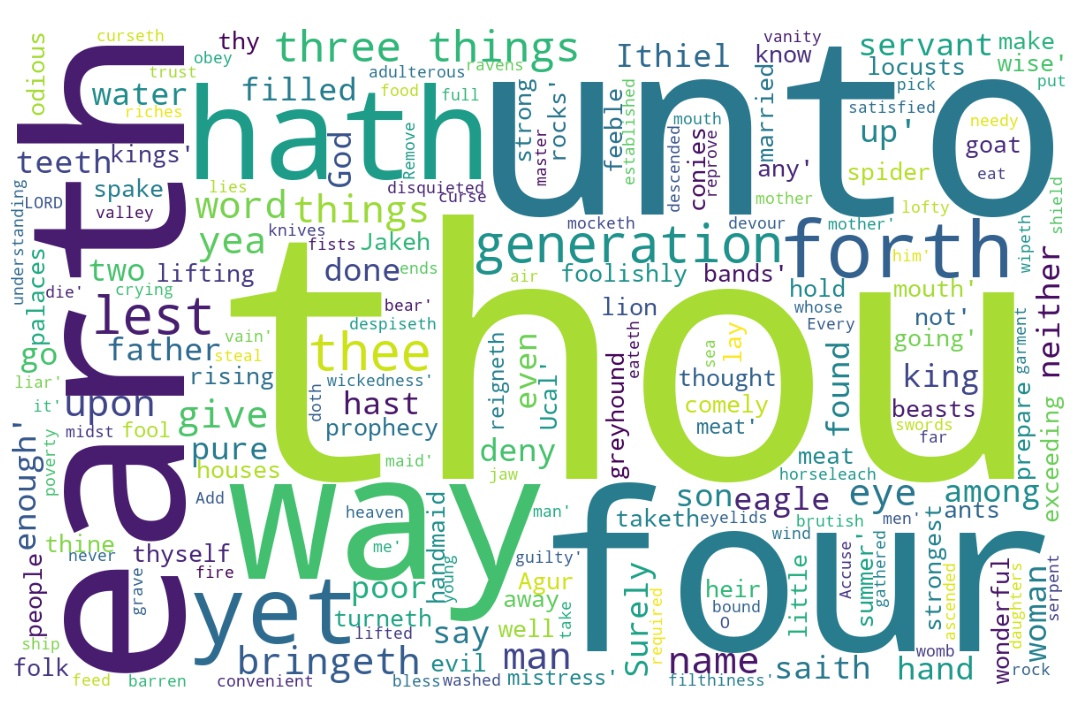
\includegraphics[width=\linewidth]{20OT-Proverbs/Proverb30-WordCloud.jpg}
  \caption{Proverb 30 Word Cloud}
  \label{fig:Proverb 30 word Cloud}
\end{figure}


\marginpar{\scriptsize \centering \fcolorbox{bone}{lime}{\textbf{A CONVERT TO WISDOM}}\\ (Proverb 30:1--33) 
\begin{compactenum}[I.][8]
    \item \textbf{Responds to Revealed Truth} \index[scripture]{Proverbs!Pro 30:01}(Pro 30:1)
    \item \textbf{Realizes his Brutish Condition} \index[scripture]{Proverbs!Pro 30:02-03}(Pro 30:2-3)
    \item \textbf{Respects God's Word} \index[scripture]{Proverbs!Pro 30:04-06}(Pro 30:4-6)
    \item \textbf{Requests Security from God} \index[scripture]{Proverbs!Pro 30:07-09}(Pro 30:7-9)
    \item Is \textbf{Repulsed by Wickedness} \index[scripture]{Proverbs!Pro 30:10-14}(Pro 30:10-14)
    \item \textbf{Recognizes Truth in Nature} \index[scripture]{Proverbs!Pro 30:15-31}(Pro 30:15-31)
    \item \textbf{Repents of Self-Promotion} \index[scripture]{Proverbs!Pro 30:32}(Pro 30:32)
\end{compactenum} }


\marginpar{\scriptsize \centering \fcolorbox{bone}{yellow}{\textbf{SEEING THE ASCENDANT ONE}}\\ (Proverb 30:1--33) 
\begin{compactenum}[I.][8]
    \item Who is \textbf{Listening} \index[scripture]{Proverbs!Pro 30:04}(Pro 30:4)
    \item Who is \textbf{Longing for Satisfaction} \index[scripture]{Proverbs!Pro 30:04}(Pro 30:4)
    \item Who is \textbf{Looking through Scripture} \index[scripture]{Proverbs!Pro 30:04}(Pro 30:4, \index[scripture]{Psalms!Psa 040:07}Psa 40:7)
    \item Who is \textbf{Laboring for Salvation} \index[scripture]{Proverbs!Pro 30:04}(Pro 30:4) -- only to find that he cannot succeed
    \item Who is \textbf{Lamenting Sin} \index[scripture]{Proverbs!Pro 30:04}(Pro 30:4) -- only to find that he cannot succeed
    \item Who is \textbf{Lost and Seeking} \index[scripture]{Proverbs!Pro 30:04}(Pro 30:4) 
    \item Who is \textbf{Lowly and Sorrowful} \index[scripture]{Proverbs!Pro 30:04}(Pro 30:4) 
\end{compactenum} }

\footnote{\textcolor[cmyk]{0.99998,1,0,0}{\hyperlink{TOC}{Return to end of Table of Contents.}}}\footnote{\href{https://www.audioverse.org/english/audiobibles/books/ENGKJV/O/Prov/1}{\textcolor[cmyk]{0.99998,1,0,0}{Proverbs Audio}}}\textcolor[cmyk]{0.99998,1,0,0}{The words of Agur the son of Jakeh, \emph{even} the \fcolorbox{bone}{lime}{prophecy}: the man spake unto Ithiel, even unto Ithiel and Ucal,}
[2] \textcolor[cmyk]{0.99998,1,0,0}{Surely I \emph{am} more \fcolorbox{bone}{lime}{brutish} than \emph{any} man, and have not the \fcolorbox{bone}{MYGOLD}{understanding} of a man.}\footnote{\textbf{Psalm 92:5-6} - O LORD, how great are thy works! and thy thoughts are very deep. [6] A brutish man knoweth not; neither doth a fool understand this.}
[3] \textcolor[cmyk]{0.99998,1,0,0}{I neither learned wisdom, nor have the knowledge of the holy.}
[4] \textcolor[cmyk]{0.99998,1,0,0}{Who hath ascended up into heaven, or descended? who hath gathered the wind in his fists? who hath bound the waters in a garment? who hath established all the ends of the earth? what \emph{is} his name, and what \emph{is} his son's name, if thou canst tell?}\footnote{\textbf{Exodus 3:13} - And Moses said unto God, Behold, when I come unto the children of Israel, and shall say unto them, The God of your fathers hath sent me unto you; and they shall say to me, What is his name? what shall I say unto them?}\footnote{\textbf{Job 26:8} - He bindeth up the waters in his thick clouds; and the cloud is not rent under them.}\footnote{\textbf{Job 38:37} - Who can number the clouds in wisdom? or who can stay the bottles of heaven,}\footnote{The connection is to the great KJV biblical truth of the Great Deep, starting back in Genesis.. The verse speaks to cosmology, or the structure of the universe. See ``garment'' in Hebrews 1:11 - They shall perish; but thou remainest; and they all shall wax old as doth a garment. See the typology pictured by the robe of a vindicated Mordecai in Esther 8:15 - And Mordecai went out from the presence of the king in royal apparel of blue and white, and with a great crown of gold, and with a garment of fine linen and purple: and the city of Shushan rejoiced and was glad. See the pure garment made of a single type of material in Deuteronomy 22:11 - Thou shalt not wear a garment of divers sorts, as of woollen and linen together. See the shepherd's garment in Jeremiah 43:12 - And I will kindle a fire in the houses of the gods of Egypt; and he shall burn them, and carry them away captives: and he shall array himself with the land of Egypt, as a shepherd putteth on his garment; and he shall go forth from thence in peace.  See the Lord's garment (the universe) described in Isaiah 50:9, 51:6, and 51:9.}
[5] \textcolor[cmyk]{0.99998,1,0,0}{Every \fcolorbox{bone}{lime}{word} of God \emph{is} pure: he \emph{is} a shield unto them that put their trust in him.}\footnote{\textbf{Psalm 12:6} - The words of the LORD are pure words: as silver tried in a furnace of earth, purified seven times.}
[6] \textcolor[cmyk]{0.99998,1,0,0}{Add thou not unto his words, lest he reprove thee, and thou be found a liar.}\footnote{\textbf{Revelation 22:18-19} -- For I testify unto every man that heareth the words of the prophecy of this book, If any man shall add unto these things, God shall add unto him the plagues that are written in this book: [19] And if any man shall take away from the words of the book of this prophecy, God shall take away his part out of the book of life, and out of the holy city, and from the things which are written in this book.}\footnote{\textbf{Deuteronomy 4:2} -- Ye shall not add unto the word which I command you, neither shall ye diminish ought from it, that ye may keep the commandments of the LORD your God which I command you.}
[7] \textcolor[cmyk]{0.99998,1,0,0}{Two \emph{things} have I \fcolorbox{bone}{lime}{required} of thee; deny me \emph{them} not before I die:}
[8] \textcolor[cmyk]{0.99998,1,0,0}{Remove far from me vanity and lies: give me neither poverty nor riches; feed me with food convenient for me:}
[9] \textcolor[cmyk]{0.99998,1,0,0}{Lest I be full, and deny \emph{thee}, and say, Who \emph{is} the LORD? or lest I be poor, and steal, and take the name of my God \emph{in} \emph{vain}.}
[10] \textcolor[cmyk]{0.99998,1,0,0}{Accuse not a servant unto his master, lest he curse thee, and thou be found guilty.}
[11] \textcolor[cmyk]{0.99998,1,0,0}{\emph{There} \emph{is} a generation \emph{that} curseth their father, and doth not bless their mother.}
[12] \textcolor[cmyk]{0.99998,1,0,0}{\fcolorbox{bone}{lime}{\emph{There} \emph{is} a generation} \emph{that} \emph{are} pure in their own eyes, and \emph{yet} is not washed from their filthiness.}
[13] \textcolor[cmyk]{0.99998,1,0,0}{\emph{There} \emph{is} a generation, O how lofty are their eyes! and their eyelids are lifted up.}
[14] \textcolor[cmyk]{0.99998,1,0,0}{\emph{There} \emph{is} a generation, whose teeth \emph{are} \emph{as} swords, and their jaw teeth \emph{as} knives, to devour the poor from off the earth, and the needy from \emph{among} men.}
[15] \textcolor[cmyk]{0.99998,1,0,0}{The \fcolorbox{bone}{lime}{horseleach} hath two daughters, \emph{crying}, Give, give. There are three \emph{things} \emph{that} are never satisfied, \emph{yea}, four \emph{things} say not, \emph{It} \emph{is} enough:}
[16] \textcolor[cmyk]{0.99998,1,0,0}{The grave; and the barren womb; the earth \emph{that} is not filled with water; and the fire \emph{that} saith not, \emph{It} \emph{is} enough.}
[17] \textcolor[cmyk]{0.99998,1,0,0}{The eye \emph{that} mocketh at \emph{his} father, and despiseth to obey \emph{his} mother, the ravens of the valley shall pick it out, and the young eagles shall eat it.}
[18] \textcolor[cmyk]{0.99998,1,0,0}{There be three \emph{things} \emph{which} are too wonderful for me, yea, four which I know not:}
[19] \textcolor[cmyk]{0.99998,1,0,0}{The way of an eagle in the air; the way of a serpent upon a rock; the way of a ship in the midst of the sea; and the way of a man with a maid.}
[20] \textcolor[cmyk]{0.99998,1,0,0}{Such \emph{is} the way of an adulterous woman; she eateth, and wipeth her mouth, and saith, I have done no wickedness.}
[21] \textcolor[cmyk]{0.99998,1,0,0}{For three \emph{things} the earth is disquieted, and for four \emph{which} it cannot bear:}
[22] \textcolor[cmyk]{0.99998,1,0,0}{For a servant when he reigneth; and a fool when he is filled with meat;}
[23] \textcolor[cmyk]{0.99998,1,0,0}{For an odious \emph{woman} when she is married; and an handmaid that is heir to her mistress.}
[24] \textcolor[cmyk]{0.99998,1,0,0}{There be four \emph{things} \emph{which} \emph{are} little upon the earth, but they \emph{are} exceeding wise:}
[25] \textcolor[cmyk]{0.99998,1,0,0}{The ants \emph{are} a people not strong, yet they prepare their meat in the summer;}
[26] \textcolor[cmyk]{0.99998,1,0,0}{The conies \emph{are} \emph{but} a feeble folk, yet make they their houses in the rocks;}
[27] \textcolor[cmyk]{0.99998,1,0,0}{The locusts have no king, yet go they forth all of them by bands;}
[28] \textcolor[cmyk]{0.99998,1,0,0}{The spider taketh hold with her hands, and is in kings' palaces.}
[29] \textcolor[cmyk]{0.99998,1,0,0}{There be three \emph{things} which go well, yea, four are comely in going:}
[30] \textcolor[cmyk]{0.99998,1,0,0}{A lion \emph{which} \emph{is} strongest among beasts, and turneth not away for any;}
[31] \textcolor[cmyk]{0.99998,1,0,0}{A greyhound; an he goat also; and a king, against whom \emph{there} \emph{is} no rising up.}
[32] \textcolor[cmyk]{0.99998,1,0,0}{If thou hast done foolishly in \fcolorbox{bone}{lime}{lifting up thyself}, or if thou hast thought evil, \emph{lay} thine hand upon thy mouth.}
[33] \textcolor[cmyk]{0.99998,1,0,0}{Surely the churning of milk bringeth forth butter, and the wringing of the nose bringeth forth blood: so the forcing of wrath bringeth forth strife.}


\index[NWIV]{21!Proverbs!Pro 30:1}\index[AWIP]{The!Proverbs!Pro 30:1}\index[AWIP]{words!Proverbs!Pro 30:1}\index[AWIP]{of!Proverbs!Pro 30:1}\index[AWIP]{of!Proverbs!Pro 30:1 (2)}\index[AWIP]{Agur!Proverbs!Pro 30:1}\index[AWIP]{the!Proverbs!Pro 30:1}\index[AWIP]{the!Proverbs!Pro 30:1 (2)}\index[AWIP]{the!Proverbs!Pro 30:1 (3)}\index[AWIP]{son!Proverbs!Pro 30:1}\index[AWIP]{Jakeh!Proverbs!Pro 30:1}\index[AWIP]{\emph{even}!Proverbs!Pro 30:1}\index[AWIP]{prophecy!Proverbs!Pro 30:1}\index[AWIP]{man!Proverbs!Pro 30:1}\index[AWIP]{spake!Proverbs!Pro 30:1}\index[AWIP]{unto!Proverbs!Pro 30:1}\index[AWIP]{unto!Proverbs!Pro 30:1 (2)}\index[AWIP]{Ithiel!Proverbs!Pro 30:1}\index[AWIP]{Ithiel!Proverbs!Pro 30:1 (2)}\index[AWIP]{even!Proverbs!Pro 30:1}\index[AWIP]{and!Proverbs!Pro 30:1}\index[AWIP]{Ucal!Proverbs!Pro 30:1}\index[AWIP]{\emph{even}!Proverbs!Pro 30:1}

\index[NWIV]{16!Proverbs!Pro 30:2}\index[AWIP]{Surely!Proverbs!Pro 30:2}\index[AWIP]{I!Proverbs!Pro 30:2}\index[AWIP]{\emph{am}!Proverbs!Pro 30:2}\index[AWIP]{more!Proverbs!Pro 30:2}\index[AWIP]{brutish!Proverbs!Pro 30:2}\index[AWIP]{than!Proverbs!Pro 30:2}\index[AWIP]{\emph{any}!Proverbs!Pro 30:2}\index[AWIP]{man!Proverbs!Pro 30:2}\index[AWIP]{man!Proverbs!Pro 30:2 (2)}\index[AWIP]{and!Proverbs!Pro 30:2}\index[AWIP]{have!Proverbs!Pro 30:2}\index[AWIP]{not!Proverbs!Pro 30:2}\index[AWIP]{the!Proverbs!Pro 30:2}\index[AWIP]{understanding!Proverbs!Pro 30:2}\index[AWIP]{of!Proverbs!Pro 30:2}\index[AWIP]{a!Proverbs!Pro 30:2}\index[AWIP]{\emph{am}!Proverbs!Pro 30:2}\index[AWIP]{\emph{any}!Proverbs!Pro 30:2}

\index[NWIV]{11!Proverbs!Pro 30:3}\index[AWIP]{I!Proverbs!Pro 30:3}\index[AWIP]{neither!Proverbs!Pro 30:3}\index[AWIP]{learned!Proverbs!Pro 30:3}\index[AWIP]{wisdom!Proverbs!Pro 30:3}\index[AWIP]{nor!Proverbs!Pro 30:3}\index[AWIP]{have!Proverbs!Pro 30:3}\index[AWIP]{the!Proverbs!Pro 30:3}\index[AWIP]{the!Proverbs!Pro 30:3 (2)}\index[AWIP]{knowledge!Proverbs!Pro 30:3}\index[AWIP]{of!Proverbs!Pro 30:3}\index[AWIP]{holy!Proverbs!Pro 30:3}

\index[NWIV]{47!Proverbs!Pro 30:4}\index[AWIP]{Who!Proverbs!Pro 30:4}\index[AWIP]{hath!Proverbs!Pro 30:4}\index[AWIP]{hath!Proverbs!Pro 30:4 (2)}\index[AWIP]{hath!Proverbs!Pro 30:4 (3)}\index[AWIP]{hath!Proverbs!Pro 30:4 (4)}\index[AWIP]{ascended!Proverbs!Pro 30:4}\index[AWIP]{up!Proverbs!Pro 30:4}\index[AWIP]{into!Proverbs!Pro 30:4}\index[AWIP]{heaven!Proverbs!Pro 30:4}\index[AWIP]{or!Proverbs!Pro 30:4}\index[AWIP]{descended?!Proverbs!Pro 30:4}\index[AWIP]{who!Proverbs!Pro 30:4}\index[AWIP]{who!Proverbs!Pro 30:4 (2)}\index[AWIP]{who!Proverbs!Pro 30:4 (3)}\index[AWIP]{gathered!Proverbs!Pro 30:4}\index[AWIP]{the!Proverbs!Pro 30:4}\index[AWIP]{the!Proverbs!Pro 30:4 (2)}\index[AWIP]{the!Proverbs!Pro 30:4 (3)}\index[AWIP]{the!Proverbs!Pro 30:4 (4)}\index[AWIP]{wind!Proverbs!Pro 30:4}\index[AWIP]{in!Proverbs!Pro 30:4}\index[AWIP]{in!Proverbs!Pro 30:4 (2)}\index[AWIP]{his!Proverbs!Pro 30:4}\index[AWIP]{his!Proverbs!Pro 30:4 (2)}\index[AWIP]{his!Proverbs!Pro 30:4 (3)}\index[AWIP]{fists?!Proverbs!Pro 30:4}\index[AWIP]{bound!Proverbs!Pro 30:4}\index[AWIP]{waters!Proverbs!Pro 30:4}\index[AWIP]{a!Proverbs!Pro 30:4}\index[AWIP]{garment?!Proverbs!Pro 30:4}\index[AWIP]{established!Proverbs!Pro 30:4}\index[AWIP]{all!Proverbs!Pro 30:4}\index[AWIP]{ends!Proverbs!Pro 30:4}\index[AWIP]{of!Proverbs!Pro 30:4}\index[AWIP]{earth?!Proverbs!Pro 30:4}\index[AWIP]{what!Proverbs!Pro 30:4}\index[AWIP]{what!Proverbs!Pro 30:4 (2)}\index[AWIP]{\emph{is}!Proverbs!Pro 30:4}\index[AWIP]{\emph{is}!Proverbs!Pro 30:4 (2)}\index[AWIP]{name!Proverbs!Pro 30:4}\index[AWIP]{name!Proverbs!Pro 30:4 (2)}\index[AWIP]{and!Proverbs!Pro 30:4}\index[AWIP]{son's!Proverbs!Pro 30:4}\index[AWIP]{if!Proverbs!Pro 30:4}\index[AWIP]{thou!Proverbs!Pro 30:4}\index[AWIP]{canst!Proverbs!Pro 30:4}\index[AWIP]{tell?!Proverbs!Pro 30:4}\index[AWIP]{\emph{is}!Proverbs!Pro 30:4}\index[AWIP]{\emph{is}!Proverbs!Pro 30:4 (2)}

\index[NWIV]{18!Proverbs!Pro 30:5}\index[AWIP]{Every!Proverbs!Pro 30:5}\index[AWIP]{word!Proverbs!Pro 30:5}\index[AWIP]{of!Proverbs!Pro 30:5}\index[AWIP]{God!Proverbs!Pro 30:5}\index[AWIP]{\emph{is}!Proverbs!Pro 30:5}\index[AWIP]{\emph{is}!Proverbs!Pro 30:5 (2)}\index[AWIP]{pure!Proverbs!Pro 30:5}\index[AWIP]{he!Proverbs!Pro 30:5}\index[AWIP]{a!Proverbs!Pro 30:5}\index[AWIP]{shield!Proverbs!Pro 30:5}\index[AWIP]{unto!Proverbs!Pro 30:5}\index[AWIP]{them!Proverbs!Pro 30:5}\index[AWIP]{that!Proverbs!Pro 30:5}\index[AWIP]{put!Proverbs!Pro 30:5}\index[AWIP]{their!Proverbs!Pro 30:5}\index[AWIP]{trust!Proverbs!Pro 30:5}\index[AWIP]{in!Proverbs!Pro 30:5}\index[AWIP]{him!Proverbs!Pro 30:5}\index[AWIP]{\emph{is}!Proverbs!Pro 30:5}\index[AWIP]{\emph{is}!Proverbs!Pro 30:5 (2)}

\index[NWIV]{16!Proverbs!Pro 30:6}\index[AWIP]{Add!Proverbs!Pro 30:6}\index[AWIP]{thou!Proverbs!Pro 30:6}\index[AWIP]{thou!Proverbs!Pro 30:6 (2)}\index[AWIP]{not!Proverbs!Pro 30:6}\index[AWIP]{unto!Proverbs!Pro 30:6}\index[AWIP]{his!Proverbs!Pro 30:6}\index[AWIP]{words!Proverbs!Pro 30:6}\index[AWIP]{lest!Proverbs!Pro 30:6}\index[AWIP]{he!Proverbs!Pro 30:6}\index[AWIP]{reprove!Proverbs!Pro 30:6}\index[AWIP]{thee!Proverbs!Pro 30:6}\index[AWIP]{and!Proverbs!Pro 30:6}\index[AWIP]{be!Proverbs!Pro 30:6}\index[AWIP]{found!Proverbs!Pro 30:6}\index[AWIP]{a!Proverbs!Pro 30:6}\index[AWIP]{liar!Proverbs!Pro 30:6}

\index[NWIV]{14!Proverbs!Pro 30:7}\index[AWIP]{Two!Proverbs!Pro 30:7}\index[AWIP]{\emph{things}!Proverbs!Pro 30:7}\index[AWIP]{have!Proverbs!Pro 30:7}\index[AWIP]{I!Proverbs!Pro 30:7}\index[AWIP]{I!Proverbs!Pro 30:7 (2)}\index[AWIP]{required!Proverbs!Pro 30:7}\index[AWIP]{of!Proverbs!Pro 30:7}\index[AWIP]{thee!Proverbs!Pro 30:7}\index[AWIP]{deny!Proverbs!Pro 30:7}\index[AWIP]{me!Proverbs!Pro 30:7}\index[AWIP]{\emph{them}!Proverbs!Pro 30:7}\index[AWIP]{not!Proverbs!Pro 30:7}\index[AWIP]{before!Proverbs!Pro 30:7}\index[AWIP]{die!Proverbs!Pro 30:7}\index[AWIP]{\emph{things}!Proverbs!Pro 30:7}\index[AWIP]{\emph{them}!Proverbs!Pro 30:7}

\index[NWIV]{20!Proverbs!Pro 30:8}\index[AWIP]{Remove!Proverbs!Pro 30:8}\index[AWIP]{far!Proverbs!Pro 30:8}\index[AWIP]{from!Proverbs!Pro 30:8}\index[AWIP]{me!Proverbs!Pro 30:8}\index[AWIP]{me!Proverbs!Pro 30:8 (2)}\index[AWIP]{me!Proverbs!Pro 30:8 (3)}\index[AWIP]{me!Proverbs!Pro 30:8 (4)}\index[AWIP]{vanity!Proverbs!Pro 30:8}\index[AWIP]{and!Proverbs!Pro 30:8}\index[AWIP]{lies!Proverbs!Pro 30:8}\index[AWIP]{give!Proverbs!Pro 30:8}\index[AWIP]{neither!Proverbs!Pro 30:8}\index[AWIP]{poverty!Proverbs!Pro 30:8}\index[AWIP]{nor!Proverbs!Pro 30:8}\index[AWIP]{riches!Proverbs!Pro 30:8}\index[AWIP]{feed!Proverbs!Pro 30:8}\index[AWIP]{with!Proverbs!Pro 30:8}\index[AWIP]{food!Proverbs!Pro 30:8}\index[AWIP]{convenient!Proverbs!Pro 30:8}\index[AWIP]{for!Proverbs!Pro 30:8}

\index[NWIV]{29!Proverbs!Pro 30:9}\index[AWIP]{Lest!Proverbs!Pro 30:9}\index[AWIP]{I!Proverbs!Pro 30:9}\index[AWIP]{I!Proverbs!Pro 30:9 (2)}\index[AWIP]{be!Proverbs!Pro 30:9}\index[AWIP]{be!Proverbs!Pro 30:9 (2)}\index[AWIP]{full!Proverbs!Pro 30:9}\index[AWIP]{and!Proverbs!Pro 30:9}\index[AWIP]{and!Proverbs!Pro 30:9 (2)}\index[AWIP]{and!Proverbs!Pro 30:9 (3)}\index[AWIP]{and!Proverbs!Pro 30:9 (4)}\index[AWIP]{deny!Proverbs!Pro 30:9}\index[AWIP]{\emph{thee}!Proverbs!Pro 30:9}\index[AWIP]{say!Proverbs!Pro 30:9}\index[AWIP]{Who!Proverbs!Pro 30:9}\index[AWIP]{\emph{is}!Proverbs!Pro 30:9}\index[AWIP]{the!Proverbs!Pro 30:9}\index[AWIP]{the!Proverbs!Pro 30:9 (2)}\index[AWIP]{LORD?!Proverbs!Pro 30:9}\index[AWIP]{or!Proverbs!Pro 30:9}\index[AWIP]{lest!Proverbs!Pro 30:9}\index[AWIP]{poor!Proverbs!Pro 30:9}\index[AWIP]{steal!Proverbs!Pro 30:9}\index[AWIP]{take!Proverbs!Pro 30:9}\index[AWIP]{name!Proverbs!Pro 30:9}\index[AWIP]{of!Proverbs!Pro 30:9}\index[AWIP]{my!Proverbs!Pro 30:9}\index[AWIP]{God!Proverbs!Pro 30:9}\index[AWIP]{\emph{in}!Proverbs!Pro 30:9}\index[AWIP]{\emph{vain}!Proverbs!Pro 30:9}\index[AWIP]{\emph{thee}!Proverbs!Pro 30:9}\index[AWIP]{\emph{is}!Proverbs!Pro 30:9}\index[AWIP]{\emph{in}!Proverbs!Pro 30:9}\index[AWIP]{\emph{vain}!Proverbs!Pro 30:9}

\index[NWIV]{16!Proverbs!Pro 30:10}\index[AWIP]{Accuse!Proverbs!Pro 30:10}\index[AWIP]{not!Proverbs!Pro 30:10}\index[AWIP]{a!Proverbs!Pro 30:10}\index[AWIP]{servant!Proverbs!Pro 30:10}\index[AWIP]{unto!Proverbs!Pro 30:10}\index[AWIP]{his!Proverbs!Pro 30:10}\index[AWIP]{master!Proverbs!Pro 30:10}\index[AWIP]{lest!Proverbs!Pro 30:10}\index[AWIP]{he!Proverbs!Pro 30:10}\index[AWIP]{curse!Proverbs!Pro 30:10}\index[AWIP]{thee!Proverbs!Pro 30:10}\index[AWIP]{and!Proverbs!Pro 30:10}\index[AWIP]{thou!Proverbs!Pro 30:10}\index[AWIP]{be!Proverbs!Pro 30:10}\index[AWIP]{found!Proverbs!Pro 30:10}\index[AWIP]{guilty!Proverbs!Pro 30:10}

\index[NWIV]{14!Proverbs!Pro 30:11}\index[AWIP]{\emph{There}!Proverbs!Pro 30:11}\index[AWIP]{\emph{is}!Proverbs!Pro 30:11}\index[AWIP]{a!Proverbs!Pro 30:11}\index[AWIP]{generation!Proverbs!Pro 30:11}\index[AWIP]{\emph{that}!Proverbs!Pro 30:11}\index[AWIP]{curseth!Proverbs!Pro 30:11}\index[AWIP]{their!Proverbs!Pro 30:11}\index[AWIP]{their!Proverbs!Pro 30:11 (2)}\index[AWIP]{father!Proverbs!Pro 30:11}\index[AWIP]{and!Proverbs!Pro 30:11}\index[AWIP]{doth!Proverbs!Pro 30:11}\index[AWIP]{not!Proverbs!Pro 30:11}\index[AWIP]{bless!Proverbs!Pro 30:11}\index[AWIP]{mother!Proverbs!Pro 30:11}\index[AWIP]{\emph{There}!Proverbs!Pro 30:11}\index[AWIP]{\emph{is}!Proverbs!Pro 30:11}\index[AWIP]{\emph{that}!Proverbs!Pro 30:11}

\index[NWIV]{19!Proverbs!Pro 30:12}\index[AWIP]{\emph{There}!Proverbs!Pro 30:12}\index[AWIP]{\emph{is}!Proverbs!Pro 30:12}\index[AWIP]{a!Proverbs!Pro 30:12}\index[AWIP]{generation!Proverbs!Pro 30:12}\index[AWIP]{\emph{that}!Proverbs!Pro 30:12}\index[AWIP]{\emph{are}!Proverbs!Pro 30:12}\index[AWIP]{pure!Proverbs!Pro 30:12}\index[AWIP]{in!Proverbs!Pro 30:12}\index[AWIP]{their!Proverbs!Pro 30:12}\index[AWIP]{their!Proverbs!Pro 30:12 (2)}\index[AWIP]{own!Proverbs!Pro 30:12}\index[AWIP]{eyes!Proverbs!Pro 30:12}\index[AWIP]{and!Proverbs!Pro 30:12}\index[AWIP]{\emph{yet}!Proverbs!Pro 30:12}\index[AWIP]{is!Proverbs!Pro 30:12}\index[AWIP]{not!Proverbs!Pro 30:12}\index[AWIP]{washed!Proverbs!Pro 30:12}\index[AWIP]{from!Proverbs!Pro 30:12}\index[AWIP]{filthiness!Proverbs!Pro 30:12}\index[AWIP]{\emph{There}!Proverbs!Pro 30:12}\index[AWIP]{\emph{is}!Proverbs!Pro 30:12}\index[AWIP]{\emph{that}!Proverbs!Pro 30:12}\index[AWIP]{\emph{are}!Proverbs!Pro 30:12}\index[AWIP]{\emph{yet}!Proverbs!Pro 30:12}

\index[NWIV]{16!Proverbs!Pro 30:13}\index[AWIP]{\emph{There}!Proverbs!Pro 30:13}\index[AWIP]{\emph{is}!Proverbs!Pro 30:13}\index[AWIP]{a!Proverbs!Pro 30:13}\index[AWIP]{generation!Proverbs!Pro 30:13}\index[AWIP]{O!Proverbs!Pro 30:13}\index[AWIP]{how!Proverbs!Pro 30:13}\index[AWIP]{lofty!Proverbs!Pro 30:13}\index[AWIP]{are!Proverbs!Pro 30:13}\index[AWIP]{are!Proverbs!Pro 30:13 (2)}\index[AWIP]{their!Proverbs!Pro 30:13}\index[AWIP]{their!Proverbs!Pro 30:13 (2)}\index[AWIP]{eyes!!Proverbs!Pro 30:13}\index[AWIP]{and!Proverbs!Pro 30:13}\index[AWIP]{eyelids!Proverbs!Pro 30:13}\index[AWIP]{lifted!Proverbs!Pro 30:13}\index[AWIP]{up!Proverbs!Pro 30:13}\index[AWIP]{\emph{There}!Proverbs!Pro 30:13}\index[AWIP]{\emph{is}!Proverbs!Pro 30:13}

\index[NWIV]{29!Proverbs!Pro 30:14}\index[AWIP]{\emph{There}!Proverbs!Pro 30:14}\index[AWIP]{\emph{is}!Proverbs!Pro 30:14}\index[AWIP]{a!Proverbs!Pro 30:14}\index[AWIP]{generation!Proverbs!Pro 30:14}\index[AWIP]{whose!Proverbs!Pro 30:14}\index[AWIP]{teeth!Proverbs!Pro 30:14}\index[AWIP]{teeth!Proverbs!Pro 30:14 (2)}\index[AWIP]{\emph{are}!Proverbs!Pro 30:14}\index[AWIP]{\emph{as}!Proverbs!Pro 30:14}\index[AWIP]{\emph{as}!Proverbs!Pro 30:14 (2)}\index[AWIP]{swords!Proverbs!Pro 30:14}\index[AWIP]{and!Proverbs!Pro 30:14}\index[AWIP]{and!Proverbs!Pro 30:14 (2)}\index[AWIP]{their!Proverbs!Pro 30:14}\index[AWIP]{jaw!Proverbs!Pro 30:14}\index[AWIP]{knives!Proverbs!Pro 30:14}\index[AWIP]{to!Proverbs!Pro 30:14}\index[AWIP]{devour!Proverbs!Pro 30:14}\index[AWIP]{the!Proverbs!Pro 30:14}\index[AWIP]{the!Proverbs!Pro 30:14 (2)}\index[AWIP]{the!Proverbs!Pro 30:14 (3)}\index[AWIP]{poor!Proverbs!Pro 30:14}\index[AWIP]{from!Proverbs!Pro 30:14}\index[AWIP]{from!Proverbs!Pro 30:14 (2)}\index[AWIP]{off!Proverbs!Pro 30:14}\index[AWIP]{earth!Proverbs!Pro 30:14}\index[AWIP]{needy!Proverbs!Pro 30:14}\index[AWIP]{\emph{among}!Proverbs!Pro 30:14}\index[AWIP]{men!Proverbs!Pro 30:14}\index[AWIP]{\emph{There}!Proverbs!Pro 30:14}\index[AWIP]{\emph{is}!Proverbs!Pro 30:14}\index[AWIP]{\emph{are}!Proverbs!Pro 30:14}\index[AWIP]{\emph{as}!Proverbs!Pro 30:14}\index[AWIP]{\emph{as}!Proverbs!Pro 30:14 (2)}\index[AWIP]{\emph{among}!Proverbs!Pro 30:14}

\index[NWIV]{24!Proverbs!Pro 30:15}\index[AWIP]{The!Proverbs!Pro 30:15}\index[AWIP]{horseleach!Proverbs!Pro 30:15}\index[AWIP]{hath!Proverbs!Pro 30:15}\index[AWIP]{two!Proverbs!Pro 30:15}\index[AWIP]{daughters!Proverbs!Pro 30:15}\index[AWIP]{\emph{crying}!Proverbs!Pro 30:15}\index[AWIP]{Give!Proverbs!Pro 30:15}\index[AWIP]{give!Proverbs!Pro 30:15}\index[AWIP]{There!Proverbs!Pro 30:15}\index[AWIP]{are!Proverbs!Pro 30:15}\index[AWIP]{are!Proverbs!Pro 30:15 (2)}\index[AWIP]{three!Proverbs!Pro 30:15}\index[AWIP]{\emph{things}!Proverbs!Pro 30:15}\index[AWIP]{\emph{things}!Proverbs!Pro 30:15 (2)}\index[AWIP]{\emph{that}!Proverbs!Pro 30:15}\index[AWIP]{never!Proverbs!Pro 30:15}\index[AWIP]{satisfied!Proverbs!Pro 30:15}\index[AWIP]{\emph{yea}!Proverbs!Pro 30:15}\index[AWIP]{four!Proverbs!Pro 30:15}\index[AWIP]{say!Proverbs!Pro 30:15}\index[AWIP]{not!Proverbs!Pro 30:15}\index[AWIP]{\emph{It}!Proverbs!Pro 30:15}\index[AWIP]{\emph{is}!Proverbs!Pro 30:15}\index[AWIP]{enough!Proverbs!Pro 30:15}\index[AWIP]{\emph{crying}!Proverbs!Pro 30:15}\index[AWIP]{\emph{things}!Proverbs!Pro 30:15}\index[AWIP]{\emph{things}!Proverbs!Pro 30:15 (2)}\index[AWIP]{\emph{that}!Proverbs!Pro 30:15}\index[AWIP]{\emph{yea}!Proverbs!Pro 30:15}\index[AWIP]{\emph{It}!Proverbs!Pro 30:15}\index[AWIP]{\emph{is}!Proverbs!Pro 30:15}

\index[NWIV]{23!Proverbs!Pro 30:16}\index[AWIP]{The!Proverbs!Pro 30:16}\index[AWIP]{grave!Proverbs!Pro 30:16}\index[AWIP]{and!Proverbs!Pro 30:16}\index[AWIP]{and!Proverbs!Pro 30:16 (2)}\index[AWIP]{the!Proverbs!Pro 30:16}\index[AWIP]{the!Proverbs!Pro 30:16 (2)}\index[AWIP]{the!Proverbs!Pro 30:16 (3)}\index[AWIP]{barren!Proverbs!Pro 30:16}\index[AWIP]{womb!Proverbs!Pro 30:16}\index[AWIP]{earth!Proverbs!Pro 30:16}\index[AWIP]{\emph{that}!Proverbs!Pro 30:16}\index[AWIP]{\emph{that}!Proverbs!Pro 30:16 (2)}\index[AWIP]{is!Proverbs!Pro 30:16}\index[AWIP]{not!Proverbs!Pro 30:16}\index[AWIP]{not!Proverbs!Pro 30:16 (2)}\index[AWIP]{filled!Proverbs!Pro 30:16}\index[AWIP]{with!Proverbs!Pro 30:16}\index[AWIP]{water!Proverbs!Pro 30:16}\index[AWIP]{fire!Proverbs!Pro 30:16}\index[AWIP]{saith!Proverbs!Pro 30:16}\index[AWIP]{\emph{It}!Proverbs!Pro 30:16}\index[AWIP]{\emph{is}!Proverbs!Pro 30:16}\index[AWIP]{enough!Proverbs!Pro 30:16}\index[AWIP]{\emph{that}!Proverbs!Pro 30:16}\index[AWIP]{\emph{that}!Proverbs!Pro 30:16 (2)}\index[AWIP]{\emph{It}!Proverbs!Pro 30:16}\index[AWIP]{\emph{is}!Proverbs!Pro 30:16}

\index[NWIV]{29!Proverbs!Pro 30:17}\index[AWIP]{The!Proverbs!Pro 30:17}\index[AWIP]{eye!Proverbs!Pro 30:17}\index[AWIP]{\emph{that}!Proverbs!Pro 30:17}\index[AWIP]{mocketh!Proverbs!Pro 30:17}\index[AWIP]{at!Proverbs!Pro 30:17}\index[AWIP]{\emph{his}!Proverbs!Pro 30:17}\index[AWIP]{\emph{his}!Proverbs!Pro 30:17 (2)}\index[AWIP]{father!Proverbs!Pro 30:17}\index[AWIP]{and!Proverbs!Pro 30:17}\index[AWIP]{and!Proverbs!Pro 30:17 (2)}\index[AWIP]{despiseth!Proverbs!Pro 30:17}\index[AWIP]{to!Proverbs!Pro 30:17}\index[AWIP]{obey!Proverbs!Pro 30:17}\index[AWIP]{mother!Proverbs!Pro 30:17}\index[AWIP]{the!Proverbs!Pro 30:17}\index[AWIP]{the!Proverbs!Pro 30:17 (2)}\index[AWIP]{the!Proverbs!Pro 30:17 (3)}\index[AWIP]{ravens!Proverbs!Pro 30:17}\index[AWIP]{of!Proverbs!Pro 30:17}\index[AWIP]{valley!Proverbs!Pro 30:17}\index[AWIP]{shall!Proverbs!Pro 30:17}\index[AWIP]{shall!Proverbs!Pro 30:17 (2)}\index[AWIP]{pick!Proverbs!Pro 30:17}\index[AWIP]{it!Proverbs!Pro 30:17}\index[AWIP]{it!Proverbs!Pro 30:17 (2)}\index[AWIP]{out!Proverbs!Pro 30:17}\index[AWIP]{young!Proverbs!Pro 30:17}\index[AWIP]{eagles!Proverbs!Pro 30:17}\index[AWIP]{eat!Proverbs!Pro 30:17}\index[AWIP]{\emph{that}!Proverbs!Pro 30:17}\index[AWIP]{\emph{his}!Proverbs!Pro 30:17}\index[AWIP]{\emph{his}!Proverbs!Pro 30:17 (2)}

\index[NWIV]{16!Proverbs!Pro 30:18}\index[AWIP]{There!Proverbs!Pro 30:18}\index[AWIP]{be!Proverbs!Pro 30:18}\index[AWIP]{three!Proverbs!Pro 30:18}\index[AWIP]{\emph{things}!Proverbs!Pro 30:18}\index[AWIP]{\emph{which}!Proverbs!Pro 30:18}\index[AWIP]{are!Proverbs!Pro 30:18}\index[AWIP]{too!Proverbs!Pro 30:18}\index[AWIP]{wonderful!Proverbs!Pro 30:18}\index[AWIP]{for!Proverbs!Pro 30:18}\index[AWIP]{me!Proverbs!Pro 30:18}\index[AWIP]{yea!Proverbs!Pro 30:18}\index[AWIP]{four!Proverbs!Pro 30:18}\index[AWIP]{which!Proverbs!Pro 30:18}\index[AWIP]{I!Proverbs!Pro 30:18}\index[AWIP]{know!Proverbs!Pro 30:18}\index[AWIP]{not!Proverbs!Pro 30:18}\index[AWIP]{\emph{things}!Proverbs!Pro 30:18}\index[AWIP]{\emph{which}!Proverbs!Pro 30:18}

\index[NWIV]{36!Proverbs!Pro 30:19}\index[AWIP]{The!Proverbs!Pro 30:19}\index[AWIP]{way!Proverbs!Pro 30:19}\index[AWIP]{way!Proverbs!Pro 30:19 (2)}\index[AWIP]{way!Proverbs!Pro 30:19 (3)}\index[AWIP]{way!Proverbs!Pro 30:19 (4)}\index[AWIP]{of!Proverbs!Pro 30:19}\index[AWIP]{of!Proverbs!Pro 30:19 (2)}\index[AWIP]{of!Proverbs!Pro 30:19 (3)}\index[AWIP]{of!Proverbs!Pro 30:19 (4)}\index[AWIP]{of!Proverbs!Pro 30:19 (5)}\index[AWIP]{an!Proverbs!Pro 30:19}\index[AWIP]{eagle!Proverbs!Pro 30:19}\index[AWIP]{in!Proverbs!Pro 30:19}\index[AWIP]{in!Proverbs!Pro 30:19 (2)}\index[AWIP]{the!Proverbs!Pro 30:19}\index[AWIP]{the!Proverbs!Pro 30:19 (2)}\index[AWIP]{the!Proverbs!Pro 30:19 (3)}\index[AWIP]{the!Proverbs!Pro 30:19 (4)}\index[AWIP]{the!Proverbs!Pro 30:19 (5)}\index[AWIP]{the!Proverbs!Pro 30:19 (6)}\index[AWIP]{air!Proverbs!Pro 30:19}\index[AWIP]{a!Proverbs!Pro 30:19}\index[AWIP]{a!Proverbs!Pro 30:19 (2)}\index[AWIP]{a!Proverbs!Pro 30:19 (3)}\index[AWIP]{a!Proverbs!Pro 30:19 (4)}\index[AWIP]{a!Proverbs!Pro 30:19 (5)}\index[AWIP]{serpent!Proverbs!Pro 30:19}\index[AWIP]{upon!Proverbs!Pro 30:19}\index[AWIP]{rock!Proverbs!Pro 30:19}\index[AWIP]{ship!Proverbs!Pro 30:19}\index[AWIP]{midst!Proverbs!Pro 30:19}\index[AWIP]{sea!Proverbs!Pro 30:19}\index[AWIP]{and!Proverbs!Pro 30:19}\index[AWIP]{man!Proverbs!Pro 30:19}\index[AWIP]{with!Proverbs!Pro 30:19}\index[AWIP]{maid!Proverbs!Pro 30:19}

\index[NWIV]{21!Proverbs!Pro 30:20}\index[AWIP]{Such!Proverbs!Pro 30:20}\index[AWIP]{\emph{is}!Proverbs!Pro 30:20}\index[AWIP]{the!Proverbs!Pro 30:20}\index[AWIP]{way!Proverbs!Pro 30:20}\index[AWIP]{of!Proverbs!Pro 30:20}\index[AWIP]{an!Proverbs!Pro 30:20}\index[AWIP]{adulterous!Proverbs!Pro 30:20}\index[AWIP]{woman!Proverbs!Pro 30:20}\index[AWIP]{she!Proverbs!Pro 30:20}\index[AWIP]{eateth!Proverbs!Pro 30:20}\index[AWIP]{and!Proverbs!Pro 30:20}\index[AWIP]{and!Proverbs!Pro 30:20 (2)}\index[AWIP]{wipeth!Proverbs!Pro 30:20}\index[AWIP]{her!Proverbs!Pro 30:20}\index[AWIP]{mouth!Proverbs!Pro 30:20}\index[AWIP]{saith!Proverbs!Pro 30:20}\index[AWIP]{I!Proverbs!Pro 30:20}\index[AWIP]{have!Proverbs!Pro 30:20}\index[AWIP]{done!Proverbs!Pro 30:20}\index[AWIP]{no!Proverbs!Pro 30:20}\index[AWIP]{wickedness!Proverbs!Pro 30:20}\index[AWIP]{\emph{is}!Proverbs!Pro 30:20}

\index[NWIV]{14!Proverbs!Pro 30:21}\index[AWIP]{For!Proverbs!Pro 30:21}\index[AWIP]{three!Proverbs!Pro 30:21}\index[AWIP]{\emph{things}!Proverbs!Pro 30:21}\index[AWIP]{the!Proverbs!Pro 30:21}\index[AWIP]{earth!Proverbs!Pro 30:21}\index[AWIP]{is!Proverbs!Pro 30:21}\index[AWIP]{disquieted!Proverbs!Pro 30:21}\index[AWIP]{and!Proverbs!Pro 30:21}\index[AWIP]{for!Proverbs!Pro 30:21}\index[AWIP]{four!Proverbs!Pro 30:21}\index[AWIP]{\emph{which}!Proverbs!Pro 30:21}\index[AWIP]{it!Proverbs!Pro 30:21}\index[AWIP]{cannot!Proverbs!Pro 30:21}\index[AWIP]{bear!Proverbs!Pro 30:21}\index[AWIP]{\emph{things}!Proverbs!Pro 30:21}\index[AWIP]{\emph{which}!Proverbs!Pro 30:21}

\index[NWIV]{15!Proverbs!Pro 30:22}\index[AWIP]{For!Proverbs!Pro 30:22}\index[AWIP]{a!Proverbs!Pro 30:22}\index[AWIP]{a!Proverbs!Pro 30:22 (2)}\index[AWIP]{servant!Proverbs!Pro 30:22}\index[AWIP]{when!Proverbs!Pro 30:22}\index[AWIP]{when!Proverbs!Pro 30:22 (2)}\index[AWIP]{he!Proverbs!Pro 30:22}\index[AWIP]{he!Proverbs!Pro 30:22 (2)}\index[AWIP]{reigneth!Proverbs!Pro 30:22}\index[AWIP]{and!Proverbs!Pro 30:22}\index[AWIP]{fool!Proverbs!Pro 30:22}\index[AWIP]{is!Proverbs!Pro 30:22}\index[AWIP]{filled!Proverbs!Pro 30:22}\index[AWIP]{with!Proverbs!Pro 30:22}\index[AWIP]{meat!Proverbs!Pro 30:22}

\index[NWIV]{17!Proverbs!Pro 30:23}\index[AWIP]{For!Proverbs!Pro 30:23}\index[AWIP]{an!Proverbs!Pro 30:23}\index[AWIP]{an!Proverbs!Pro 30:23 (2)}\index[AWIP]{odious!Proverbs!Pro 30:23}\index[AWIP]{\emph{woman}!Proverbs!Pro 30:23}\index[AWIP]{when!Proverbs!Pro 30:23}\index[AWIP]{she!Proverbs!Pro 30:23}\index[AWIP]{is!Proverbs!Pro 30:23}\index[AWIP]{is!Proverbs!Pro 30:23 (2)}\index[AWIP]{married!Proverbs!Pro 30:23}\index[AWIP]{and!Proverbs!Pro 30:23}\index[AWIP]{handmaid!Proverbs!Pro 30:23}\index[AWIP]{that!Proverbs!Pro 30:23}\index[AWIP]{heir!Proverbs!Pro 30:23}\index[AWIP]{to!Proverbs!Pro 30:23}\index[AWIP]{her!Proverbs!Pro 30:23}\index[AWIP]{mistress!Proverbs!Pro 30:23}\index[AWIP]{\emph{woman}!Proverbs!Pro 30:23}

\index[NWIV]{15!Proverbs!Pro 30:24}\index[AWIP]{There!Proverbs!Pro 30:24}\index[AWIP]{be!Proverbs!Pro 30:24}\index[AWIP]{four!Proverbs!Pro 30:24}\index[AWIP]{\emph{things}!Proverbs!Pro 30:24}\index[AWIP]{\emph{which}!Proverbs!Pro 30:24}\index[AWIP]{\emph{are}!Proverbs!Pro 30:24}\index[AWIP]{\emph{are}!Proverbs!Pro 30:24 (2)}\index[AWIP]{little!Proverbs!Pro 30:24}\index[AWIP]{upon!Proverbs!Pro 30:24}\index[AWIP]{the!Proverbs!Pro 30:24}\index[AWIP]{earth!Proverbs!Pro 30:24}\index[AWIP]{but!Proverbs!Pro 30:24}\index[AWIP]{they!Proverbs!Pro 30:24}\index[AWIP]{exceeding!Proverbs!Pro 30:24}\index[AWIP]{wise!Proverbs!Pro 30:24}\index[AWIP]{\emph{things}!Proverbs!Pro 30:24}\index[AWIP]{\emph{which}!Proverbs!Pro 30:24}\index[AWIP]{\emph{are}!Proverbs!Pro 30:24}\index[AWIP]{\emph{are}!Proverbs!Pro 30:24 (2)}

\index[NWIV]{15!Proverbs!Pro 30:25}\index[AWIP]{The!Proverbs!Pro 30:25}\index[AWIP]{ants!Proverbs!Pro 30:25}\index[AWIP]{\emph{are}!Proverbs!Pro 30:25}\index[AWIP]{a!Proverbs!Pro 30:25}\index[AWIP]{people!Proverbs!Pro 30:25}\index[AWIP]{not!Proverbs!Pro 30:25}\index[AWIP]{strong!Proverbs!Pro 30:25}\index[AWIP]{yet!Proverbs!Pro 30:25}\index[AWIP]{they!Proverbs!Pro 30:25}\index[AWIP]{prepare!Proverbs!Pro 30:25}\index[AWIP]{their!Proverbs!Pro 30:25}\index[AWIP]{meat!Proverbs!Pro 30:25}\index[AWIP]{in!Proverbs!Pro 30:25}\index[AWIP]{the!Proverbs!Pro 30:25}\index[AWIP]{summer!Proverbs!Pro 30:25}\index[AWIP]{\emph{are}!Proverbs!Pro 30:25}

\index[NWIV]{15!Proverbs!Pro 30:26}\index[AWIP]{The!Proverbs!Pro 30:26}\index[AWIP]{conies!Proverbs!Pro 30:26}\index[AWIP]{\emph{are}!Proverbs!Pro 30:26}\index[AWIP]{\emph{but}!Proverbs!Pro 30:26}\index[AWIP]{a!Proverbs!Pro 30:26}\index[AWIP]{feeble!Proverbs!Pro 30:26}\index[AWIP]{folk!Proverbs!Pro 30:26}\index[AWIP]{yet!Proverbs!Pro 30:26}\index[AWIP]{make!Proverbs!Pro 30:26}\index[AWIP]{they!Proverbs!Pro 30:26}\index[AWIP]{their!Proverbs!Pro 30:26}\index[AWIP]{houses!Proverbs!Pro 30:26}\index[AWIP]{in!Proverbs!Pro 30:26}\index[AWIP]{the!Proverbs!Pro 30:26}\index[AWIP]{rocks!Proverbs!Pro 30:26}\index[AWIP]{\emph{are}!Proverbs!Pro 30:26}\index[AWIP]{\emph{but}!Proverbs!Pro 30:26}

\index[NWIV]{14!Proverbs!Pro 30:27}\index[AWIP]{The!Proverbs!Pro 30:27}\index[AWIP]{locusts!Proverbs!Pro 30:27}\index[AWIP]{have!Proverbs!Pro 30:27}\index[AWIP]{no!Proverbs!Pro 30:27}\index[AWIP]{king!Proverbs!Pro 30:27}\index[AWIP]{yet!Proverbs!Pro 30:27}\index[AWIP]{go!Proverbs!Pro 30:27}\index[AWIP]{they!Proverbs!Pro 30:27}\index[AWIP]{forth!Proverbs!Pro 30:27}\index[AWIP]{all!Proverbs!Pro 30:27}\index[AWIP]{of!Proverbs!Pro 30:27}\index[AWIP]{them!Proverbs!Pro 30:27}\index[AWIP]{by!Proverbs!Pro 30:27}\index[AWIP]{bands!Proverbs!Pro 30:27}

\index[NWIV]{12!Proverbs!Pro 30:28}\index[AWIP]{The!Proverbs!Pro 30:28}\index[AWIP]{spider!Proverbs!Pro 30:28}\index[AWIP]{taketh!Proverbs!Pro 30:28}\index[AWIP]{hold!Proverbs!Pro 30:28}\index[AWIP]{with!Proverbs!Pro 30:28}\index[AWIP]{her!Proverbs!Pro 30:28}\index[AWIP]{hands!Proverbs!Pro 30:28}\index[AWIP]{and!Proverbs!Pro 30:28}\index[AWIP]{is!Proverbs!Pro 30:28}\index[AWIP]{in!Proverbs!Pro 30:28}\index[AWIP]{kings'!Proverbs!Pro 30:28}\index[AWIP]{palaces!Proverbs!Pro 30:28}

\index[NWIV]{13!Proverbs!Pro 30:29}\index[AWIP]{There!Proverbs!Pro 30:29}\index[AWIP]{be!Proverbs!Pro 30:29}\index[AWIP]{three!Proverbs!Pro 30:29}\index[AWIP]{\emph{things}!Proverbs!Pro 30:29}\index[AWIP]{which!Proverbs!Pro 30:29}\index[AWIP]{go!Proverbs!Pro 30:29}\index[AWIP]{well!Proverbs!Pro 30:29}\index[AWIP]{yea!Proverbs!Pro 30:29}\index[AWIP]{four!Proverbs!Pro 30:29}\index[AWIP]{are!Proverbs!Pro 30:29}\index[AWIP]{comely!Proverbs!Pro 30:29}\index[AWIP]{in!Proverbs!Pro 30:29}\index[AWIP]{going!Proverbs!Pro 30:29}\index[AWIP]{\emph{things}!Proverbs!Pro 30:29}

\index[NWIV]{13!Proverbs!Pro 30:30}\index[AWIP]{A!Proverbs!Pro 30:30}\index[AWIP]{lion!Proverbs!Pro 30:30}\index[AWIP]{\emph{which}!Proverbs!Pro 30:30}\index[AWIP]{\emph{is}!Proverbs!Pro 30:30}\index[AWIP]{strongest!Proverbs!Pro 30:30}\index[AWIP]{among!Proverbs!Pro 30:30}\index[AWIP]{beasts!Proverbs!Pro 30:30}\index[AWIP]{and!Proverbs!Pro 30:30}\index[AWIP]{turneth!Proverbs!Pro 30:30}\index[AWIP]{not!Proverbs!Pro 30:30}\index[AWIP]{away!Proverbs!Pro 30:30}\index[AWIP]{for!Proverbs!Pro 30:30}\index[AWIP]{any!Proverbs!Pro 30:30}\index[AWIP]{\emph{which}!Proverbs!Pro 30:30}\index[AWIP]{\emph{is}!Proverbs!Pro 30:30}

\index[NWIV]{16!Proverbs!Pro 30:31}\index[AWIP]{A!Proverbs!Pro 30:31}\index[AWIP]{greyhound!Proverbs!Pro 30:31}\index[AWIP]{an!Proverbs!Pro 30:31}\index[AWIP]{he!Proverbs!Pro 30:31}\index[AWIP]{goat!Proverbs!Pro 30:31}\index[AWIP]{also!Proverbs!Pro 30:31}\index[AWIP]{and!Proverbs!Pro 30:31}\index[AWIP]{a!Proverbs!Pro 30:31}\index[AWIP]{king!Proverbs!Pro 30:31}\index[AWIP]{against!Proverbs!Pro 30:31}\index[AWIP]{whom!Proverbs!Pro 30:31}\index[AWIP]{\emph{there}!Proverbs!Pro 30:31}\index[AWIP]{\emph{is}!Proverbs!Pro 30:31}\index[AWIP]{no!Proverbs!Pro 30:31}\index[AWIP]{rising!Proverbs!Pro 30:31}\index[AWIP]{up!Proverbs!Pro 30:31}\index[AWIP]{\emph{there}!Proverbs!Pro 30:31}\index[AWIP]{\emph{is}!Proverbs!Pro 30:31}

\index[NWIV]{21!Proverbs!Pro 30:32}\index[AWIP]{If!Proverbs!Pro 30:32}\index[AWIP]{thou!Proverbs!Pro 30:32}\index[AWIP]{thou!Proverbs!Pro 30:32 (2)}\index[AWIP]{hast!Proverbs!Pro 30:32}\index[AWIP]{hast!Proverbs!Pro 30:32 (2)}\index[AWIP]{done!Proverbs!Pro 30:32}\index[AWIP]{foolishly!Proverbs!Pro 30:32}\index[AWIP]{in!Proverbs!Pro 30:32}\index[AWIP]{lifting!Proverbs!Pro 30:32}\index[AWIP]{up!Proverbs!Pro 30:32}\index[AWIP]{thyself!Proverbs!Pro 30:32}\index[AWIP]{or!Proverbs!Pro 30:32}\index[AWIP]{if!Proverbs!Pro 30:32}\index[AWIP]{thought!Proverbs!Pro 30:32}\index[AWIP]{evil!Proverbs!Pro 30:32}\index[AWIP]{\emph{lay}!Proverbs!Pro 30:32}\index[AWIP]{thine!Proverbs!Pro 30:32}\index[AWIP]{hand!Proverbs!Pro 30:32}\index[AWIP]{upon!Proverbs!Pro 30:32}\index[AWIP]{thy!Proverbs!Pro 30:32}\index[AWIP]{mouth!Proverbs!Pro 30:32}\index[AWIP]{\emph{lay}!Proverbs!Pro 30:32}

\index[NWIV]{25!Proverbs!Pro 30:33}\index[AWIP]{Surely!Proverbs!Pro 30:33}\index[AWIP]{the!Proverbs!Pro 30:33}\index[AWIP]{the!Proverbs!Pro 30:33 (2)}\index[AWIP]{the!Proverbs!Pro 30:33 (3)}\index[AWIP]{the!Proverbs!Pro 30:33 (4)}\index[AWIP]{churning!Proverbs!Pro 30:33}\index[AWIP]{of!Proverbs!Pro 30:33}\index[AWIP]{of!Proverbs!Pro 30:33 (2)}\index[AWIP]{of!Proverbs!Pro 30:33 (3)}\index[AWIP]{milk!Proverbs!Pro 30:33}\index[AWIP]{bringeth!Proverbs!Pro 30:33}\index[AWIP]{bringeth!Proverbs!Pro 30:33 (2)}\index[AWIP]{bringeth!Proverbs!Pro 30:33 (3)}\index[AWIP]{forth!Proverbs!Pro 30:33}\index[AWIP]{forth!Proverbs!Pro 30:33 (2)}\index[AWIP]{forth!Proverbs!Pro 30:33 (3)}\index[AWIP]{butter!Proverbs!Pro 30:33}\index[AWIP]{and!Proverbs!Pro 30:33}\index[AWIP]{wringing!Proverbs!Pro 30:33}\index[AWIP]{nose!Proverbs!Pro 30:33}\index[AWIP]{blood!Proverbs!Pro 30:33}\index[AWIP]{so!Proverbs!Pro 30:33}\index[AWIP]{forcing!Proverbs!Pro 30:33}\index[AWIP]{wrath!Proverbs!Pro 30:33}\index[AWIP]{strife!Proverbs!Pro 30:33}


\section{Proverb 30 Outlines}

\subsection{My Outlines}

\subsubsection{A Convert to Wisdom}
\textbf{Introduction:} Proverbs 30.
\index[speaker]{Keith Anthony!Proverb 30 (A Convert to Wisdom)}
\index[series]{Proverbs (Keith Anthony)!Pro 30 (A Convert to Wisdom)}
\index[date]{2016/05/29!Proverb 30 (A Convert to Wisdom) (Keith Anthony)}
\begin{compactenum}[I.][7]
    \item \textbf{Responds to Revealed Truth} \index[scripture]{Proverbs!Pro 30:01}(Pro 30:1)
    \item \textbf{Realizes his Brutish Condition} \index[scripture]{Proverbs!Pro 30:02-03}(Pro 30:2-3)
    \item \textbf{Respects God's Word} \index[scripture]{Proverbs!Pro 30:04-06}(Pro 30:4-6)
    \item \textbf{Requests Security from God} \index[scripture]{Proverbs!Pro 30:07-09}(Pro 30:7-9)
    \item Is \textbf{Repulsed by Wickedness} \index[scripture]{Proverbs!Pro 30:10-14}(Pro 30:10-14)
    \item \textbf{Recognizes Truth in Nature} \index[scripture]{Proverbs!Pro 30:15-31}(Pro 30:15-31)
    \item \textbf{Repents of Self-Promotion} \index[scripture]{Proverbs!Pro 30:32}(Pro 30:32)
\end{compactenum}

\subsubsection{Seeing the Ascendant One}
\textbf{Introduction:} Who can tell who this is? The one who:\
\index[speaker]{Keith Anthony!Proverb 30 (Seeing the Ascendant One)}
\index[series]{Proverbs (Keith Anthony)!Pro 30:04 (Seeing the Ascendant One)}
\index[date]{2016/05/29!Proverb 30:04 (Seeing the Ascendant One) (Keith Anthony)}
\begin{compactenum}[I.][7]
    \item Who is \textbf{Listening} \index[scripture]{Proverbs!Pro 30:04}(Pro 30:4)
    \item Who is \textbf{Longing for Satisfaction} \index[scripture]{Proverbs!Pro 30:04}(Pro 30:4)
    \item Who is \textbf{Looking through Scripture} \index[scripture]{Proverbs!Pro 30:04}(Pro 30:4, \index[scripture]{Psalms!Psa 040:07}Psa 40:7)
    \item Who is \textbf{Laboring for Salvation} \index[scripture]{Proverbs!Pro 30:04}(Pro 30:4) -- only to find that he cannot succeed
    \item Who is \textbf{Lamenting Sin} \index[scripture]{Proverbs!Pro 30:04}(Pro 30:4) -- only to find that he cannot succeed
    \item Who is \textbf{Lost and Seeking} \index[scripture]{Proverbs!Pro 30:04}(Pro 30:4) 
    \item Who is \textbf{Lowly and Sorrowful} \index[scripture]{Proverbs!Pro 30:04}(Pro 30:4) 
\end{compactenum}


\subsection{Outlines from Clarence Billheimer}


\subsubsection{Characteristics of a Faithful Christian}

\index[speaker]{Clarence Billheimer!Proverb 30:24-28 (Characteristics of a Faithful Christian)}
\index[series]{Proverbs (Clarence Billheimer)!Pro 30:24-28 (Characteristics of a Faithful Christian)}
\index[date]{2020/09/02!Proverb 30:24-28 (Characteristics of a Faithful Christian) (Clarence Billheimer)}

\noindent  \textbf{Introduction: } You might wonder why I chose this text for a message. It’s one of the observations of life and nature that the inspired writer of Proverbs noticed. That’s the reason I chose it. As the writer looked at these creations of God, he noticed some things about them which God created within them that we can apply to our lives if we want to be faithful, and be in a way like these creatures. They would not survive without the instincts God gave them, and we can’t be faithful if we lack the like characteristics.\\
\\
\begin{compactenum}[I.]
    \item The dedication of the ant
    \begin{compactenum}[A.]
	    \item A people not strong
	    \item Prepares for the future
	    \item Procures his need with diligence
	    \item Application—we don’t need a lot of strength to be prepared and diligent.
	\end{compactenum}
    \item The dependence of the coney
    \begin{compactenum}[A.]
	    \item Realizes his feebleness
	    \item Runs to the rocks for shelter and safety
	    \item Receives needed protection
	    \item Application—we need to depend on God and build on the Rock, Christ Jesus.
		\end{compactenum}
    \item The determination of the locust
    \begin{compactenum}[A.]
	    \item Working together
	    \item Wreaking havoc
	    \item Weaken what they consume
	    \item Application—we need to work together to accomplish the complete mission God gave us.
		\end{compactenum}
    \item The delicacy of the spider
    \begin{compactenum}[A.]
	    \item Found in festive places
	    \item Found in family placed
	    \item Feared by his prey
	    \item Application—Jesus said, “Be wise as serpents and harmless as doves.”\\
	\end{compactenum}
\end{compactenum}

\noindent  \textbf{Conclusion: } A Christian will be most faithful to God when he’s dedicated to Him, dependent on Him, determined for Him, and delicate in his behavior so he’s not an offense or stumbling block.


\index[FACEBOOK]{FUNDAMENTAL BAPTIST SERMON OUTLINES!Clarence Billheimer - Proverb 30:24-28!2020/09/02}


\subsection{Outlines from Richard Drummond}

\subsubsection{What Rebellion Does}

\index[speaker]{Richard Drummond!Proverb 30:11 (What Rebellion Does)}
\index[series]{Proverbs (Richard Drummond)!Pro 30:11 (What Rebellion Does)}
\index[date]{2013/12/08!Proverb 30:11 (What Rebellion Does) (Richard Drummond)}

\noindent \textbf{Introduction: } Friends make this life much more enjoyable. There is nothing like serving the Lord with brothers and sisters in Christ. Maybe you fish, hunt, or enjoy other types of activities with those you cherish in this life. We all have special people in our lives that we love to spend time with; however, our best friend should always be the Lord Jesus Christ. In times of trouble, grief, sorrow, and despair, Jesus has been there for you and I. In times of joy, happiness, excitement, and gain, Jesus has been there for you and I!
Notice several things with me about this friendship you and I ought to cherish:
%
\begin{compactenum}[I.][8]
    \item Rebellion in the church will \textbf{Discourage} %\index[scripture]{Proverbs!Proverbs 30:04}(Proverbs 30:4)
    \item Rebellion in the church will \textbf{Destroy} relationships in the church%\index[scripture]{Proverbs!Proverbs 30:04}(Proverbs 30:4)
    \item Rebellion in the church will cause \textbf{Division} %\index[scripture]{Proverbs!Proverbs 30:04}(Proverbs 30:4)
    \item Rebellion can cause \textbf{Death} %\index[scripture]{Proverbs!Proverbs 30:04}(Proverbs 30:4)
\end{compactenum}



\index[LOCATION]{Lebanon Baptist Temple (Drummond) (What Rebellion Does)!2013/12/08!Sunday Night}


\subsection{Outlines from Travis Price}


\subsubsection{Things Every Generation Needs to Learn}

\index[speaker]{Travis Price!Proverb 30:11-33 (Things Every Generation Needs to Learns)}
\index[series]{Proverbs (Travis Price)!Pro 30:11-33 (Things Every Generation Needs to Learn)}
\index[date]{2018/09/01!Prov. 30:11-33 (Things Every Generation Needs to Learn) (Travis Price)}

\noindent  \textbf{Introduction: } (Vs 11-14) 4 times "generation" is mentioned.\\

\begin{compactenum}[I.]
    \item MISCONTENTED THINGS (Vs 15-7)
    \item MYSTIFYING THINGS (Vs 18-20)
    \item MISERABLE THINGS (Vs 21-23)
    \item MARVELOUS THINGS (Vs 24-28)
    \item MAJESTIC THINGS (Vs 29-31)\\
\end{compactenum}
Final 2 verses personal plea of action



\index[FACEBOOK]{ALLITERATED SERMON OUTLINES!Travis Price - Proverb 30:11-33!2018/09/01}


\section{Proverb 30 Comments}

\subsection{Numeric Nuggets}
\textbf{13:} Verses 29 and 30 have 13 words. Verses 7, 11, 29, and 30 contain 13 unique words. There is a single 13-letter word in Proverb 30: ``understanding.'' Proverb 30:29 and  30:30 contain 13 words. 

\textbf{4:} The phrase ``There is a generation'' is found four times.


\subsection{Proverb 30 Repeated Phrases}


%%%%%%%%%%
%%%%%%%%%%
\normalsize
 
\begin{center}
\begin{longtable}{|c|c|}
\caption[Proverb 30 Repeated Phrases]{Proverb 30 Repeated Phrases}\label{table:Repeated Phrases Proverb 30} \\
\hline \multicolumn{1}{|c|}{\textbf{Phrase}} & \multicolumn{1}{c|}{\textbf{Frequency}} \\ \hline 
\endfirsthead
 
\multicolumn{2}{c}
{{\bfseries \tablename\ \thetable{} -- continued from previous page}} \\  
\hline \multicolumn{1}{|c|}{\textbf{Phrase}} & \multicolumn{1}{c|}{\textbf{Frequency}} \\ \hline 
\endhead
 
\hline \multicolumn{2}{c}{{ }} \\ \hline
\endfoot 
and the & 6\\ \hline 
of the & 5\\ \hline 
the earth & 5\\ \hline 
\emph{is} a & 5\\ \hline 
way of & 5\\ \hline 
of a & 4\\ \hline 
\emph{There} \emph{is} & 4\\ \hline 
\emph{There} \emph{is} a & 4\\ \hline 
\emph{There} \emph{is} a generation & 4\\ \hline 
\emph{is} a generation & 4\\ \hline 
a generation & 4\\ \hline 
three \emph{things} & 4\\ \hline 
in the & 4\\ \hline 
the way & 4\\ \hline 
the way of & 4\\ \hline 
who hath & 3\\ \hline 
There be & 3\\ \hline 
the way of a & 3\\ \hline 
way of a & 3\\ \hline 
bringeth forth & 3\\ \hline 
\end{longtable}
\end{center}



%%%%%%%%%%
%%%%%%%%%%



%\newpage
\section{Proverb 3 Statistics}

%%%%%%%%%%%%%%%%%%%%%%%%%%%
%%%%% Word Statistics
%%%%%%%%%%%%%%%%%%%%%%%%%%

\normalsize
\subsection{Chapter Word Statistics}


%%%%%%%%%%
%%%%%%%%%%
 
\begin{center}
\begin{longtable}{l|c|c|c|c}
\caption[Stats for Proverb 30]{Stats for Proverb 30} \label{table:Stats for Proverb 30} \\ 
\hline \multicolumn{1}{|c|}{\textbf{Verse(s)}} & \multicolumn{1}{|c|}{\textbf{Count}} & \multicolumn{1}{|c|}{\textbf{Unique}} & \multicolumn{1}{|c|}{\textbf{Italics}} & \multicolumn{1}{|c|}{\textbf{Uniq Italic}}  \\ \hline 
\endfirsthead
 
\multicolumn{5}{c}
{{\bfseries \tablename\ \thetable{} -- continued from previous page}} \\  
\hline \multicolumn{1}{|c|}{\textbf{Verse(s)}} & \multicolumn{1}{|c|}{\textbf{Count}} & \multicolumn{1}{|c|}{\textbf{Unique}} & \multicolumn{1}{|c|}{\textbf{Italics}} & \multicolumn{1}{|c|}{\textbf{Uniq Italic}}  \\ \hline 
\endhead
 
\hline \multicolumn{5}{|r|}{{Continued if needed}} \\ \hline
\endfoot 
1 & 21 & 16 & 1 & 1\\ \hline
2 & 16 & 15 & 2 & 2\\ \hline
3 & 11 & 10 & 0 & 0\\ \hline
4 & 47 & 33 & 2 & 1\\ \hline
5 & 18 & 17 & 2 & 1\\ \hline
6 & 16 & 15 & 0 & 0\\ \hline
7 & 14 & 13 & 2 & 2\\ \hline
8 & 20 & 17 & 0 & 0\\ \hline
9 & 29 & 23 & 4 & 4\\ \hline
10 & 16 & 16 & 0 & 0\\ \hline
11 & 14 & 13 & 3 & 3\\ \hline
12 & 19 & 18 & 5 & 5\\ \hline
13 & 16 & 14 & 2 & 2\\ \hline
14 & 29 & 23 & 6 & 5\\ \hline
15 & 24 & 22 & 7 & 6\\ \hline
16 & 23 & 18 & 4 & 3\\ \hline
17 & 29 & 23 & 3 & 2\\ \hline
18 & 16 & 16 & 2 & 2\\ \hline
19 & 36 & 19 & 0 & 0\\ \hline
20 & 21 & 20 & 1 & 1\\ \hline
21 & 14 & 14 & 2 & 2\\ \hline
22 & 15 & 12 & 0 & 0\\ \hline
23 & 17 & 15 & 1 & 1\\ \hline
24 & 15 & 14 & 4 & 3\\ \hline
25 & 15 & 15 & 1 & 1\\ \hline
26 & 15 & 15 & 2 & 2\\ \hline
27 & 14 & 14 & 0 & 0\\ \hline
28 & 12 & 12 & 0 & 0\\ \hline
29 & 13 & 13 & 1 & 1\\ \hline
30 & 13 & 13 & 2 & 2\\ \hline
31 & 16 & 16 & 2 & 2\\ \hline
32 & 21 & 19 & 1 & 1\\ \hline
33 & 25 & 16 & 0 & 0\\ \hline
\hline \hline
Total & 640 & 298 & 62 & 24




\end{longtable}
\end{center}

%%%%%%%%%%
%%%%%%%%%%


\subsection{Words by Frequency}

\begin{center}
\begin{longtable}{l|r}
\caption[Word Frequencies in Proverb 30]{Word Frequencies in Proverb 30} \label{table:WordsIn-Proverb-30} \\ 
\hline \multicolumn{1}{|c|}{\textbf{Word}} & \multicolumn{1}{c|}{\textbf{Frequency}} \\ \hline 
\endfirsthead
  
\multicolumn{2}{c}  
{{\bfseries \tablename\ \thetable{} -- continued from previous page}} \\   
\hline \multicolumn{1}{|c|}{\textbf{Word}} & \multicolumn{1}{c|}{\textbf{Frequency}} \\ \hline   
\endhead  
  
\hline \multicolumn{2}{|r|}{{Continue}} \\ \hline  
\endfoot  
  
\hline \hline  
\endlastfoot  
  
the & 36\\ \hline 
and & 29\\ \hline 
of & 19\\ \hline 
a & 19\\ \hline 
\emph{is} & 14\\ \hline 
not & 12\\ \hline 
in & 11\\ \hline 
their & 10\\ \hline 
The & 9\\ \hline 
I & 8\\ \hline 
be & 7\\ \hline 
\emph{things} & 7\\ \hline 
is & 7\\ \hline 
thou & 6\\ \hline 
he & 6\\ \hline 
me & 6\\ \hline 
\emph{that} & 6\\ \hline 
\emph{are} & 6\\ \hline 
are & 6\\ \hline 
unto & 5\\ \hline 
have & 5\\ \hline 
hath & 5\\ \hline 
his & 5\\ \hline 
earth & 5\\ \hline 
with & 5\\ \hline 
four & 5\\ \hline 
way & 5\\ \hline 
an & 5\\ \hline 
man & 4\\ \hline 
up & 4\\ \hline 
from & 4\\ \hline 
for & 4\\ \hline 
\emph{There} & 4\\ \hline 
generation & 4\\ \hline 
There & 4\\ \hline 
three & 4\\ \hline 
\emph{which} & 4\\ \hline 
they & 4\\ \hline 
forth & 4\\ \hline 
or & 3\\ \hline 
who & 3\\ \hline 
name & 3\\ \hline 
lest & 3\\ \hline 
thee & 3\\ \hline 
to & 3\\ \hline 
it & 3\\ \hline 
upon & 3\\ \hline 
her & 3\\ \hline 
no & 3\\ \hline 
For & 3\\ \hline 
when & 3\\ \hline 
yet & 3\\ \hline 
bringeth & 3\\ \hline 
words & 2\\ \hline 
Ithiel & 2\\ \hline 
Surely & 2\\ \hline 
neither & 2\\ \hline 
nor & 2\\ \hline 
Who & 2\\ \hline 
all & 2\\ \hline 
what & 2\\ \hline 
if & 2\\ \hline 
God & 2\\ \hline 
pure & 2\\ \hline 
them & 2\\ \hline 
that & 2\\ \hline 
found & 2\\ \hline 
deny & 2\\ \hline 
give & 2\\ \hline 
say & 2\\ \hline 
poor & 2\\ \hline 
servant & 2\\ \hline 
father & 2\\ \hline 
mother & 2\\ \hline 
eyes & 2\\ \hline 
teeth & 2\\ \hline 
\emph{as} & 2\\ \hline 
\emph{It} & 2\\ \hline 
enough & 2\\ \hline 
filled & 2\\ \hline 
saith & 2\\ \hline 
\emph{his} & 2\\ \hline 
shall & 2\\ \hline 
yea & 2\\ \hline 
which & 2\\ \hline 
she & 2\\ \hline 
mouth & 2\\ \hline 
done & 2\\ \hline 
meat & 2\\ \hline 
king & 2\\ \hline 
go & 2\\ \hline 
A & 2\\ \hline 
hast & 2\\ \hline 
Agur & 1\\ \hline 
son & 1\\ \hline 
Jakeh & 1\\ \hline 
\emph{even} & 1\\ \hline 
prophecy & 1\\ \hline 
spake & 1\\ \hline 
even & 1\\ \hline 
Ucal & 1\\ \hline 
\emph{am} & 1\\ \hline 
more & 1\\ \hline 
brutish & 1\\ \hline 
than & 1\\ \hline 
\emph{any} & 1\\ \hline 
understanding & 1\\ \hline 
learned & 1\\ \hline 
wisdom & 1\\ \hline 
knowledge & 1\\ \hline 
holy & 1\\ \hline 
ascended & 1\\ \hline 
into & 1\\ \hline 
heaven & 1\\ \hline 
descended & 1\\ \hline 
gathered & 1\\ \hline 
wind & 1\\ \hline 
fists & 1\\ \hline 
bound & 1\\ \hline 
waters & 1\\ \hline 
garment & 1\\ \hline 
established & 1\\ \hline 
ends & 1\\ \hline 
son's & 1\\ \hline 
canst & 1\\ \hline 
tell & 1\\ \hline 
Every & 1\\ \hline 
word & 1\\ \hline 
shield & 1\\ \hline 
put & 1\\ \hline 
trust & 1\\ \hline 
him & 1\\ \hline 
Add & 1\\ \hline 
reprove & 1\\ \hline 
liar & 1\\ \hline 
Two & 1\\ \hline 
required & 1\\ \hline 
\emph{them} & 1\\ \hline 
before & 1\\ \hline 
die & 1\\ \hline 
Remove & 1\\ \hline 
far & 1\\ \hline 
vanity & 1\\ \hline 
lies & 1\\ \hline 
poverty & 1\\ \hline 
riches & 1\\ \hline 
feed & 1\\ \hline 
food & 1\\ \hline 
convenient & 1\\ \hline 
Lest & 1\\ \hline 
full & 1\\ \hline 
\emph{thee} & 1\\ \hline 
LORD & 1\\ \hline 
steal & 1\\ \hline 
take & 1\\ \hline 
my & 1\\ \hline 
\emph{in} & 1\\ \hline 
\emph{vain} & 1\\ \hline 
Accuse & 1\\ \hline 
master & 1\\ \hline 
curse & 1\\ \hline 
guilty & 1\\ \hline 
curseth & 1\\ \hline 
doth & 1\\ \hline 
bless & 1\\ \hline 
own & 1\\ \hline 
\emph{yet} & 1\\ \hline 
washed & 1\\ \hline 
filthiness & 1\\ \hline 
O & 1\\ \hline 
how & 1\\ \hline 
lofty & 1\\ \hline 
eyelids & 1\\ \hline 
lifted & 1\\ \hline 
whose & 1\\ \hline 
swords & 1\\ \hline 
jaw & 1\\ \hline 
knives & 1\\ \hline 
devour & 1\\ \hline 
off & 1\\ \hline 
needy & 1\\ \hline 
\emph{among} & 1\\ \hline 
men & 1\\ \hline 
horseleach & 1\\ \hline 
two & 1\\ \hline 
daughters & 1\\ \hline 
\emph{crying} & 1\\ \hline 
Give & 1\\ \hline 
never & 1\\ \hline 
satisfied & 1\\ \hline 
\emph{yea} & 1\\ \hline 
grave & 1\\ \hline 
barren & 1\\ \hline 
womb & 1\\ \hline 
water & 1\\ \hline 
fire & 1\\ \hline 
eye & 1\\ \hline 
mocketh & 1\\ \hline 
at & 1\\ \hline 
despiseth & 1\\ \hline 
obey & 1\\ \hline 
ravens & 1\\ \hline 
valley & 1\\ \hline 
pick & 1\\ \hline 
out & 1\\ \hline 
young & 1\\ \hline 
eagles & 1\\ \hline 
eat & 1\\ \hline 
too & 1\\ \hline 
wonderful & 1\\ \hline 
know & 1\\ \hline 
eagle & 1\\ \hline 
air & 1\\ \hline 
serpent & 1\\ \hline 
rock & 1\\ \hline 
ship & 1\\ \hline 
midst & 1\\ \hline 
sea & 1\\ \hline 
maid & 1\\ \hline 
Such & 1\\ \hline 
adulterous & 1\\ \hline 
woman & 1\\ \hline 
eateth & 1\\ \hline 
wipeth & 1\\ \hline 
wickedness & 1\\ \hline 
disquieted & 1\\ \hline 
cannot & 1\\ \hline 
bear & 1\\ \hline 
reigneth & 1\\ \hline 
fool & 1\\ \hline 
odious & 1\\ \hline 
\emph{woman} & 1\\ \hline 
married & 1\\ \hline 
handmaid & 1\\ \hline 
heir & 1\\ \hline 
mistress & 1\\ \hline 
little & 1\\ \hline 
but & 1\\ \hline 
exceeding & 1\\ \hline 
wise & 1\\ \hline 
ants & 1\\ \hline 
people & 1\\ \hline 
strong & 1\\ \hline 
prepare & 1\\ \hline 
summer & 1\\ \hline 
conies & 1\\ \hline 
\emph{but} & 1\\ \hline 
feeble & 1\\ \hline 
folk & 1\\ \hline 
make & 1\\ \hline 
houses & 1\\ \hline 
rocks & 1\\ \hline 
locusts & 1\\ \hline 
by & 1\\ \hline 
bands & 1\\ \hline 
spider & 1\\ \hline 
taketh & 1\\ \hline 
hold & 1\\ \hline 
hands & 1\\ \hline 
kings' & 1\\ \hline 
palaces & 1\\ \hline 
well & 1\\ \hline 
comely & 1\\ \hline 
going & 1\\ \hline 
lion & 1\\ \hline 
strongest & 1\\ \hline 
among & 1\\ \hline 
beasts & 1\\ \hline 
turneth & 1\\ \hline 
away & 1\\ \hline 
any & 1\\ \hline 
greyhound & 1\\ \hline 
goat & 1\\ \hline 
also & 1\\ \hline 
against & 1\\ \hline 
whom & 1\\ \hline 
\emph{there} & 1\\ \hline 
rising & 1\\ \hline 
If & 1\\ \hline 
foolishly & 1\\ \hline 
lifting & 1\\ \hline 
thyself & 1\\ \hline 
thought & 1\\ \hline 
evil & 1\\ \hline 
\emph{lay} & 1\\ \hline 
thine & 1\\ \hline 
hand & 1\\ \hline 
thy & 1\\ \hline 
churning & 1\\ \hline 
milk & 1\\ \hline 
butter & 1\\ \hline 
wringing & 1\\ \hline 
nose & 1\\ \hline 
blood & 1\\ \hline 
so & 1\\ \hline 
forcing & 1\\ \hline 
wrath & 1\\ \hline 
strife & 1\\ \hline 
\end{longtable}  
\end{center}  


  
\normalsize  

  
  


\subsection{Words Alphabetically}

\begin{center}
\begin{longtable}{l|r}
\caption[Word Frequencies in Proverb 30]{Word Frequencies in Proverb 30} \label{table:WordsIn-Proverb-30} \\ 
\hline \multicolumn{1}{|c|}{\textbf{Word}} & \multicolumn{1}{c|}{\textbf{Frequency}} \\ \hline 
\endfirsthead
  
\multicolumn{2}{c}  
{{\bfseries \tablename\ \thetable{} -- continued from previous page}} \\   
\hline \multicolumn{1}{|c|}{\textbf{Word}} & \multicolumn{1}{c|}{\textbf{Frequency}} \\ \hline   
\endhead  
  
\hline \multicolumn{2}{|r|}{{Continue}} \\ \hline  
\endfoot  
  
\hline \hline  
\endlastfoot  
  
A & 2\\ \hline 
Accuse & 1\\ \hline 
Add & 1\\ \hline 
Agur & 1\\ \hline 
Every & 1\\ \hline 
For & 3\\ \hline 
Give & 1\\ \hline 
God & 2\\ \hline 
I & 8\\ \hline 
If & 1\\ \hline 
Ithiel & 2\\ \hline 
Jakeh & 1\\ \hline 
LORD & 1\\ \hline 
Lest & 1\\ \hline 
O & 1\\ \hline 
Remove & 1\\ \hline 
Such & 1\\ \hline 
Surely & 2\\ \hline 
The & 9\\ \hline 
There & 4\\ \hline 
Two & 1\\ \hline 
Ucal & 1\\ \hline 
Who & 2\\ \hline 
\emph{It} & 2\\ \hline 
\emph{There} & 4\\ \hline 
\emph{among} & 1\\ \hline 
\emph{am} & 1\\ \hline 
\emph{any} & 1\\ \hline 
\emph{are} & 6\\ \hline 
\emph{as} & 2\\ \hline 
\emph{but} & 1\\ \hline 
\emph{crying} & 1\\ \hline 
\emph{even} & 1\\ \hline 
\emph{his} & 2\\ \hline 
\emph{in} & 1\\ \hline 
\emph{is} & 14\\ \hline 
\emph{lay} & 1\\ \hline 
\emph{that} & 6\\ \hline 
\emph{thee} & 1\\ \hline 
\emph{them} & 1\\ \hline 
\emph{there} & 1\\ \hline 
\emph{things} & 7\\ \hline 
\emph{vain} & 1\\ \hline 
\emph{which} & 4\\ \hline 
\emph{woman} & 1\\ \hline 
\emph{yea} & 1\\ \hline 
\emph{yet} & 1\\ \hline 
a & 19\\ \hline 
adulterous & 1\\ \hline 
against & 1\\ \hline 
air & 1\\ \hline 
all & 2\\ \hline 
also & 1\\ \hline 
among & 1\\ \hline 
an & 5\\ \hline 
and & 29\\ \hline 
ants & 1\\ \hline 
any & 1\\ \hline 
are & 6\\ \hline 
ascended & 1\\ \hline 
at & 1\\ \hline 
away & 1\\ \hline 
bands & 1\\ \hline 
barren & 1\\ \hline 
be & 7\\ \hline 
bear & 1\\ \hline 
beasts & 1\\ \hline 
before & 1\\ \hline 
bless & 1\\ \hline 
blood & 1\\ \hline 
bound & 1\\ \hline 
bringeth & 3\\ \hline 
brutish & 1\\ \hline 
but & 1\\ \hline 
butter & 1\\ \hline 
by & 1\\ \hline 
cannot & 1\\ \hline 
canst & 1\\ \hline 
churning & 1\\ \hline 
comely & 1\\ \hline 
conies & 1\\ \hline 
convenient & 1\\ \hline 
curse & 1\\ \hline 
curseth & 1\\ \hline 
daughters & 1\\ \hline 
deny & 2\\ \hline 
descended & 1\\ \hline 
despiseth & 1\\ \hline 
devour & 1\\ \hline 
die & 1\\ \hline 
disquieted & 1\\ \hline 
done & 2\\ \hline 
doth & 1\\ \hline 
eagle & 1\\ \hline 
eagles & 1\\ \hline 
earth & 5\\ \hline 
eat & 1\\ \hline 
eateth & 1\\ \hline 
ends & 1\\ \hline 
enough & 2\\ \hline 
established & 1\\ \hline 
even & 1\\ \hline 
evil & 1\\ \hline 
exceeding & 1\\ \hline 
eye & 1\\ \hline 
eyelids & 1\\ \hline 
eyes & 2\\ \hline 
far & 1\\ \hline 
father & 2\\ \hline 
feeble & 1\\ \hline 
feed & 1\\ \hline 
filled & 2\\ \hline 
filthiness & 1\\ \hline 
fire & 1\\ \hline 
fists & 1\\ \hline 
folk & 1\\ \hline 
food & 1\\ \hline 
fool & 1\\ \hline 
foolishly & 1\\ \hline 
for & 4\\ \hline 
forcing & 1\\ \hline 
forth & 4\\ \hline 
found & 2\\ \hline 
four & 5\\ \hline 
from & 4\\ \hline 
full & 1\\ \hline 
garment & 1\\ \hline 
gathered & 1\\ \hline 
generation & 4\\ \hline 
give & 2\\ \hline 
go & 2\\ \hline 
goat & 1\\ \hline 
going & 1\\ \hline 
grave & 1\\ \hline 
greyhound & 1\\ \hline 
guilty & 1\\ \hline 
hand & 1\\ \hline 
handmaid & 1\\ \hline 
hands & 1\\ \hline 
hast & 2\\ \hline 
hath & 5\\ \hline 
have & 5\\ \hline 
he & 6\\ \hline 
heaven & 1\\ \hline 
heir & 1\\ \hline 
her & 3\\ \hline 
him & 1\\ \hline 
his & 5\\ \hline 
hold & 1\\ \hline 
holy & 1\\ \hline 
horseleach & 1\\ \hline 
houses & 1\\ \hline 
how & 1\\ \hline 
if & 2\\ \hline 
in & 11\\ \hline 
into & 1\\ \hline 
is & 7\\ \hline 
it & 3\\ \hline 
jaw & 1\\ \hline 
king & 2\\ \hline 
kings' & 1\\ \hline 
knives & 1\\ \hline 
know & 1\\ \hline 
knowledge & 1\\ \hline 
learned & 1\\ \hline 
lest & 3\\ \hline 
liar & 1\\ \hline 
lies & 1\\ \hline 
lifted & 1\\ \hline 
lifting & 1\\ \hline 
lion & 1\\ \hline 
little & 1\\ \hline 
locusts & 1\\ \hline 
lofty & 1\\ \hline 
maid & 1\\ \hline 
make & 1\\ \hline 
man & 4\\ \hline 
married & 1\\ \hline 
master & 1\\ \hline 
me & 6\\ \hline 
meat & 2\\ \hline 
men & 1\\ \hline 
midst & 1\\ \hline 
milk & 1\\ \hline 
mistress & 1\\ \hline 
mocketh & 1\\ \hline 
more & 1\\ \hline 
mother & 2\\ \hline 
mouth & 2\\ \hline 
my & 1\\ \hline 
name & 3\\ \hline 
needy & 1\\ \hline 
neither & 2\\ \hline 
never & 1\\ \hline 
no & 3\\ \hline 
nor & 2\\ \hline 
nose & 1\\ \hline 
not & 12\\ \hline 
obey & 1\\ \hline 
odious & 1\\ \hline 
of & 19\\ \hline 
off & 1\\ \hline 
or & 3\\ \hline 
out & 1\\ \hline 
own & 1\\ \hline 
palaces & 1\\ \hline 
people & 1\\ \hline 
pick & 1\\ \hline 
poor & 2\\ \hline 
poverty & 1\\ \hline 
prepare & 1\\ \hline 
prophecy & 1\\ \hline 
pure & 2\\ \hline 
put & 1\\ \hline 
ravens & 1\\ \hline 
reigneth & 1\\ \hline 
reprove & 1\\ \hline 
required & 1\\ \hline 
riches & 1\\ \hline 
rising & 1\\ \hline 
rock & 1\\ \hline 
rocks & 1\\ \hline 
saith & 2\\ \hline 
satisfied & 1\\ \hline 
say & 2\\ \hline 
sea & 1\\ \hline 
serpent & 1\\ \hline 
servant & 2\\ \hline 
shall & 2\\ \hline 
she & 2\\ \hline 
shield & 1\\ \hline 
ship & 1\\ \hline 
so & 1\\ \hline 
son & 1\\ \hline 
son's & 1\\ \hline 
spake & 1\\ \hline 
spider & 1\\ \hline 
steal & 1\\ \hline 
strife & 1\\ \hline 
strong & 1\\ \hline 
strongest & 1\\ \hline 
summer & 1\\ \hline 
swords & 1\\ \hline 
take & 1\\ \hline 
taketh & 1\\ \hline 
teeth & 2\\ \hline 
tell & 1\\ \hline 
than & 1\\ \hline 
that & 2\\ \hline 
the & 36\\ \hline 
thee & 3\\ \hline 
their & 10\\ \hline 
them & 2\\ \hline 
they & 4\\ \hline 
thine & 1\\ \hline 
thou & 6\\ \hline 
thought & 1\\ \hline 
three & 4\\ \hline 
thy & 1\\ \hline 
thyself & 1\\ \hline 
to & 3\\ \hline 
too & 1\\ \hline 
trust & 1\\ \hline 
turneth & 1\\ \hline 
two & 1\\ \hline 
understanding & 1\\ \hline 
unto & 5\\ \hline 
up & 4\\ \hline 
upon & 3\\ \hline 
valley & 1\\ \hline 
vanity & 1\\ \hline 
washed & 1\\ \hline 
water & 1\\ \hline 
waters & 1\\ \hline 
way & 5\\ \hline 
well & 1\\ \hline 
what & 2\\ \hline 
when & 3\\ \hline 
which & 2\\ \hline 
who & 3\\ \hline 
whom & 1\\ \hline 
whose & 1\\ \hline 
wickedness & 1\\ \hline 
wind & 1\\ \hline 
wipeth & 1\\ \hline 
wisdom & 1\\ \hline 
wise & 1\\ \hline 
with & 5\\ \hline 
woman & 1\\ \hline 
womb & 1\\ \hline 
wonderful & 1\\ \hline 
word & 1\\ \hline 
words & 2\\ \hline 
wrath & 1\\ \hline 
wringing & 1\\ \hline 
yea & 2\\ \hline 
yet & 3\\ \hline 
young & 1\\ \hline 
\end{longtable}  
\end{center}  


  
\normalsize  

  
  
\subsection{Word Lengths in Chapter} 
\normalsize 
\begin{center} 
\begin{longtable}{l|p{3.75in}} 
\caption[Words by Length in Proverb 30]{Words by Length in Proverb 30} \label{table:WordsIn-Proverb-30} \\ 
\hline \multicolumn{1}{|c|}{\textbf{Length}} & \multicolumn{1}{c|}{\textbf{Words}} \\ \hline 
\endfirsthead 
 
\multicolumn{2}{c} 
{{\bfseries \tablename\ \thetable{} -- continued from previous page}} \\ 
\hline \multicolumn{1}{|c|}{\textbf{Length}} & \multicolumn{1}{c|}{\textbf{Words}} \\ \hline 
\endhead 
 
\hline \multicolumn{2}{|r|}{{Continued}} \\ \hline 
\endfoot 
 
\hline \hline 
\endlastfoot 
1 & I, a, O, A\\ \hline 
2 & of, \emph{am}, up, or, in, \emph{is}, if, he, be, me, my, \emph{in}, is, \emph{as}, to, \emph{It}, at, it, an, no, go, by, If, so\\ \hline 
3 & The, the, son, man, and, \emph{any}, not, nor, Who, who, his, all, God, put, him, Add, Two, die, far, for, say, \emph{are}, own, \emph{yet}, how, are, jaw, off, men, two, \emph{yea}, eye, \emph{his}, out, eat, too, yea, way, air, sea, she, her, For, but, yet, \emph{but}, any, \emph{lay}, thy\\ \hline 
4 & Agur, \emph{even}, unto, even, Ucal, more, than, have, holy, hath, into, wind, ends, what, name, thou, tell, word, pure, them, that, lest, thee, liar, deny, \emph{them}, from, lies, give, feed, with, food, Lest, full, \emph{thee}, LORD, poor, take, \emph{vain}, \emph{that}, doth, eyes, Give, four, womb, fire, obey, pick, know, upon, rock, ship, maid, Such, done, bear, when, fool, meat, heir, they, wise, ants, folk, make, king, hold, well, lion, away, goat, also, whom, hast, evil, hand, milk, nose\\ \hline 
5 & words, Jakeh, spake, fists, bound, earth, son's, canst, Every, their, trust, found, steal, curse, \emph{There}, bless, lofty, whose, teeth, needy, \emph{among}, There, three, never, grave, water, saith, shall, young, \emph{which}, which, eagle, midst, woman, mouth, \emph{woman}, rocks, forth, bands, hands, going, among, \emph{there}, thine, blood, wrath\\ \hline 
6 & Ithiel, Surely, wisdom, heaven, waters, shield, \emph{things}, before, Remove, vanity, riches, Accuse, master, guilty, father, mother, washed, lifted, swords, knives, devour, \emph{crying}, enough, barren, filled, ravens, valley, eagles, eateth, wipeth, cannot, odious, little, people, strong, summer, conies, feeble, houses, spider, taketh, kings', comely, beasts, rising, butter, strife\\ \hline 
7 & brutish, neither, learned, garment, reprove, poverty, servant, curseth, eyelids, mocketh, serpent, married, prepare, locusts, palaces, turneth, against, lifting, thyself, thought, forcing\\ \hline 
8 & prophecy, ascended, gathered, required, reigneth, handmaid, mistress, churning, bringeth, wringing\\ \hline 
9 & knowledge, descended, daughters, satisfied, despiseth, wonderful, exceeding, strongest, greyhound, foolishly\\ \hline 
10 & convenient, generation, filthiness, horseleach, adulterous, wickedness, disquieted\\ \hline 
11 & established\\ \hline 
13 & understanding\\ \hline 
\end{longtable} 
\end{center} 




%%%%%%%%%%
%%%%%%%%%%
 



%%% For Indexes

%\index[DEVOTIONAL]{TGIF1!Os Hillman (Living for a Cause Greater Than Yourself) - Proverb 19:17!2021/12/21}

%\index[DEVOTIONAL]{TGIF1!Os Hillman (Living for a Cause Greater Than Yourself) - Proverb 19:17!2021/12/21}

















%%% colour: cardinal red - \textcolor[cmyk]{0,0.85,0.70,0.23}{text}


%%%% Example marginpar with a compactenum list --- green color text
%\marginpar{\scriptsize \textcolor[rgb]{0.00,0.545,0.269}{$\rightarrow$7 Abominations: 
%\begin{compactenum}
%	\item A proud look,
%	\item a lying tongue,
%	\item hands that shed innocent blood,
%	\item An heart that deviseth wicked imaginations,
%	\item feet that be swift in running to mischief,
%	\item A false witness that speaketh lies, and
%	\item he that soweth discord among brethren.
%\end{compactenum}}}



%\newpage

%\begin{mdframed}[style=MyFrame]
%\begin{center}
%\begin{longtable}{|p{.5in}|p{3.5in}|}

%\caption[Corruption Alert: Proverbs 18:1]{Corruption Alert: Proverbs 18:1} \label{table:CorruptionProv18:1} \\ 

%\hline  
%\multicolumn{1}{|c|}{\textbf{Version}} & 
%\multicolumn{1}{c|}{\textbf{Corruption}}  \\ \hline 
%\endfirsthead
 
%\multicolumn{2}{c}
%{{\bfseries \tablename\ \thetable{} -- continued from previous page}} \\  \hline  
%\multicolumn{1}{|c|}{\textbf{Version}} & 
%\multicolumn{1}{c|}{\textbf{Corruption}}  \\ \hline 
%\endhead
 
%\hline \multicolumn{2}{|r|}{{Continued on next page}} \\ \hline
%\endfoot 
%\textcolor[rgb]{0.00,0.00,1.00}{AV} & \textcolor[rgb]{0.00,0.00,1.00}{Through desire a man, having separated himself, seeketh \emph{and} intermeddleth with all wisdom.} \\ \hline
%
%ASV &  He that separateth himself seeketh his own desire, And  rageth against all sound wisdom. \\ \hline
%
%CEB &  Unfriendly people look out for themselves; they bicker with sensible people.\\ \hline
%
%ESV & Whoever isolates himself seeks his own desire;  he breaks out against all sound judgment. \\ \hline
%
%NASV &  He who separates himself seeks his own desire, He quarrels against all sound wisdom.\\ \hline
%
%MEV & He who separates himself seeks his own desire; he seeks and quarrels against all wisdom.\\ \hline
%
%NIV &  An unfriendly person pursues selfish ends and against all sound judgment starts quarrels. \\ \hline
%
%NKJV &  A man who isolates himself seeks his own desire; He rages against all wise judgment.\\ \hline
%
%RSV &  He who is estranged seeks pretexts  to break out against all sound judgment.\\ \hline

% \multicolumn{2}{p{4.3in}}{{Modern translations, such as the ASV and others, strike out the first part of the verse, concealing the intent of mankind in genewisdom clearly revealed in scripture. How wonderful is the obfuscated RSV text: ``He who is estranged seeks pretexts.'' What does THAT mean?}} \\ %\hline

%\hline

%\end{longtable}
%\end{center}

%\normalsize 
%\end{mdframed}

%\marginpar{\scriptsize \centering \fcolorbox{black}{lime}{\textbf{OUTIDE THE PLACE OF PROMISE}}\\ (Psalm 137:1--9) 
%\begin{compactenum}[I.][8]
%	\item \textbf{Plight \& Distress} \index[scripture]{Psalms!Psa 137:01} (Psalm 137:1)
%	\item The \textbf{Place Desired} \index[scripture]{Psalms!Psa 137:01} (Psalm 137:1)
%	\item \textbf{Pining \& Despiar} \index[scripture]{Psalms!Psa 137:02} (Psalm 137:2)
%	\item \textbf{Provoked \& Degraded}\index[scripture]{Psalms!Psa 137:03} (Psalm 137:3)
%	\item The \textbf{Predicament Described}\index[scripture]{Psalms!Psa 137:04} (Psalm 137:4)
%	\item A \textbf{Preference Decided}\index[scripture]{Psalms!Psa 137:06} (Psalm 137:6)
%	\item A \textbf{Prediction of Destruction}\index[scripture]{Psalms!Psa 137:08} (Psalm 137:8)
%\end{compactenum} }


%\subsection{Outlines from Others}

%\subsubsection{Words on Wisdom}
%\index[speaker]{John Battles!Proverbs 01 (Words on Wisdom)}
%\index[series]{Proverbs (John Battles)!Proverbs 01 (Words on Wisdom)}
%\index[date]{2016/01/20!Proverbs 01 (Words on Wisdom) (John Battles)}
%\textbf{Lineage}: adpated from S. Conway\\
%\textbf{Introduction}: Proverbs distinctly points out things that a fool does:
%\begin{compactenum}[I.][4]
%	\item \textbf{Welcome to Wisdom} \index[scripture]{Proverbs!Pro 01:01-09}(Proverbs 1:1-9)
%	\item \textbf{Warnings of Wisdom} \index[scripture]{Proverbs!Pro 01:10-19}(Proverbs 1:10-19).
%	\item \textbf{Woe of Wisdom} \index[scripture]{Proverbs!Pro 01:24-32}(Proverbs 1:24-32)
%	\item \textbf{Watchcare of Wisdom} \index[scripture]{Proverbs!Pro 01:33}(Proverbs 1:33).
%\end{compactenum}


%%%%% COLOR FOR MARGINPAR OUTLINES
%% 1  LIME - \marginpar{\scriptsize \centering \fcolorbox{black}{lime}{\textbf{TITLE}}\\ (Passage) 
%% 2. YELLOW - \marginpar{\scriptsize \centering \fcolorbox{black}{yellow}{\textbf{TITLE}}\\ (Passage) 
%% 3. Blue BGND, WHITE LETTERS - \marginpar{\scriptsize \centering \fcolorbox{black}{blue}{\textbf{\textcolor[cmyk]{0,0,0,0}{TITLE}}}\\ (Passage) 
%% 4. black BGND, WHITE LETTERS - \marginpar{\scriptsize \centering \fcolorbox{black}{black}{\textbf{\textcolor[cmyk]{0,0,0,0}{TITLE}}}\\ (Passage) 
%% 5. red BGND, WHITE LETTERS - \marginpar{\scriptsize \centering \fcolorbox{black}{red}{\textbf{\textcolor[cmyk]{0,0,0,0}{TITLE}}}\\ (Passage) 

%%%%%% INCLUSION OF GRAPHIC
%\newpage

%\begin{figure}
%\begin{center}
%\includegraphics[scale=0.5, angle=90]{07OT-Judges/References/b201107i1-large}
%\caption[Summary of the 13 Judges]{Summary of the 13 Judges}
%\label{fig:Summary of the 13 Judges}
%\end{center}
%\end{figure}


%%%%%%%%%%%
%%%%%%%%%%%

% SYTEMATIC THEOLOGY (10 + 2)
% Theology proper – The study of the character of God
% Angelology – The study of angels
% Biblical theology – The study of the Bible
% Christology – The study of Christ
% Ecclesiology – The study of the church
% Eschatology – The study of the end times[5]
% Hamartiology – The study of sin
% Pneumatology – The study of the Holy Spirit
% Soteriology – The study of salvation
% Theological anthropology – The study of the nature of humanity.
% ++
% Moral theology
% Bilical cosomolgy

%%%%%%%%%%%%%%
%%%%%%%%%%%%%%

% \footnote{\href{https://audiobible.com/bible/psalms_91.html}{\textcolor[cmyk]{0.99998,1,0,0}{Psalm 91 Audio}}}

% \marginpar{\scriptsize \centering \fcolorbox{black}{lime}{\textbf{JERUSALEM}}\\
% \fcolorbox{black}{lime}{\textbf{DON'T GO BACK TO EGYPT}} \\ (Isaiah 31:1--9) 

%%%%%%%%%%%%%%
%%% Extra Colors
%%% from https://latexcolor.blogspot.com/2019/10/list-of-latex-colors.html
%%%%%%%%%%%%%%
% \definecolor{champagne}{rgb}{0.97,0.91,0.81}
% \definecolor{bone}{rgb}{0.89,0.85,0.79}
%\titleJE
%

%%%%% EXAMPLE Index entry:
% \index[DOCTRINES]{Eschatology - Millennium!Psalms!Psa 069:036}

%%% for things found 13 times
%\fcolorbox{black}{bone}{TEXT}
\scriptsize

%%%%%%%%%%%%%%%%%%%%%%%%%%%%%
%Indices
%%%%%%%%%%%%%%%%%%%%%%%%%%%%%

\chapter{Indexes}

\printindex[DOCTRINES]
\printindex[scripture]

\printindex[speaker]
%\printindex[series]

\printindex[FACEBOOK]
\printindex[LOCATION]

\printindex[AWIP]


\printbibliography
\end{document}

